% Options for packages loaded elsewhere
\PassOptionsToPackage{unicode}{hyperref}
\PassOptionsToPackage{hyphens}{url}
%
\documentclass[
  11pt,
  letterpaper,
]{scrbook}

\usepackage{amsmath,amssymb}
\usepackage{iftex}
\ifPDFTeX
  \usepackage[T1]{fontenc}
  \usepackage[utf8]{inputenc}
  \usepackage{textcomp} % provide euro and other symbols
\else % if luatex or xetex
  \usepackage{unicode-math}
  \defaultfontfeatures{Scale=MatchLowercase}
  \defaultfontfeatures[\rmfamily]{Ligatures=TeX,Scale=1}
\fi
\usepackage{lmodern}
\ifPDFTeX\else  
    % xetex/luatex font selection
\fi
% Use upquote if available, for straight quotes in verbatim environments
\IfFileExists{upquote.sty}{\usepackage{upquote}}{}
\IfFileExists{microtype.sty}{% use microtype if available
  \usepackage[]{microtype}
  \UseMicrotypeSet[protrusion]{basicmath} % disable protrusion for tt fonts
}{}
\makeatletter
\@ifundefined{KOMAClassName}{% if non-KOMA class
  \IfFileExists{parskip.sty}{%
    \usepackage{parskip}
  }{% else
    \setlength{\parindent}{0pt}
    \setlength{\parskip}{6pt plus 2pt minus 1pt}}
}{% if KOMA class
  \KOMAoptions{parskip=half}}
\makeatother
\usepackage{xcolor}
\setlength{\emergencystretch}{3em} % prevent overfull lines
\setcounter{secnumdepth}{5}
% Make \paragraph and \subparagraph free-standing
\makeatletter
\ifx\paragraph\undefined\else
  \let\oldparagraph\paragraph
  \renewcommand{\paragraph}{
    \@ifstar
      \xxxParagraphStar
      \xxxParagraphNoStar
  }
  \newcommand{\xxxParagraphStar}[1]{\oldparagraph*{#1}\mbox{}}
  \newcommand{\xxxParagraphNoStar}[1]{\oldparagraph{#1}\mbox{}}
\fi
\ifx\subparagraph\undefined\else
  \let\oldsubparagraph\subparagraph
  \renewcommand{\subparagraph}{
    \@ifstar
      \xxxSubParagraphStar
      \xxxSubParagraphNoStar
  }
  \newcommand{\xxxSubParagraphStar}[1]{\oldsubparagraph*{#1}\mbox{}}
  \newcommand{\xxxSubParagraphNoStar}[1]{\oldsubparagraph{#1}\mbox{}}
\fi
\makeatother

\usepackage{color}
\usepackage{fancyvrb}
\newcommand{\VerbBar}{|}
\newcommand{\VERB}{\Verb[commandchars=\\\{\}]}
\DefineVerbatimEnvironment{Highlighting}{Verbatim}{commandchars=\\\{\}}
% Add ',fontsize=\small' for more characters per line
\usepackage{framed}
\definecolor{shadecolor}{RGB}{241,243,245}
\newenvironment{Shaded}{\begin{snugshade}}{\end{snugshade}}
\newcommand{\AlertTok}[1]{\textcolor[rgb]{0.68,0.00,0.00}{#1}}
\newcommand{\AnnotationTok}[1]{\textcolor[rgb]{0.37,0.37,0.37}{#1}}
\newcommand{\AttributeTok}[1]{\textcolor[rgb]{0.40,0.45,0.13}{#1}}
\newcommand{\BaseNTok}[1]{\textcolor[rgb]{0.68,0.00,0.00}{#1}}
\newcommand{\BuiltInTok}[1]{\textcolor[rgb]{0.00,0.23,0.31}{#1}}
\newcommand{\CharTok}[1]{\textcolor[rgb]{0.13,0.47,0.30}{#1}}
\newcommand{\CommentTok}[1]{\textcolor[rgb]{0.37,0.37,0.37}{#1}}
\newcommand{\CommentVarTok}[1]{\textcolor[rgb]{0.37,0.37,0.37}{\textit{#1}}}
\newcommand{\ConstantTok}[1]{\textcolor[rgb]{0.56,0.35,0.01}{#1}}
\newcommand{\ControlFlowTok}[1]{\textcolor[rgb]{0.00,0.23,0.31}{\textbf{#1}}}
\newcommand{\DataTypeTok}[1]{\textcolor[rgb]{0.68,0.00,0.00}{#1}}
\newcommand{\DecValTok}[1]{\textcolor[rgb]{0.68,0.00,0.00}{#1}}
\newcommand{\DocumentationTok}[1]{\textcolor[rgb]{0.37,0.37,0.37}{\textit{#1}}}
\newcommand{\ErrorTok}[1]{\textcolor[rgb]{0.68,0.00,0.00}{#1}}
\newcommand{\ExtensionTok}[1]{\textcolor[rgb]{0.00,0.23,0.31}{#1}}
\newcommand{\FloatTok}[1]{\textcolor[rgb]{0.68,0.00,0.00}{#1}}
\newcommand{\FunctionTok}[1]{\textcolor[rgb]{0.28,0.35,0.67}{#1}}
\newcommand{\ImportTok}[1]{\textcolor[rgb]{0.00,0.46,0.62}{#1}}
\newcommand{\InformationTok}[1]{\textcolor[rgb]{0.37,0.37,0.37}{#1}}
\newcommand{\KeywordTok}[1]{\textcolor[rgb]{0.00,0.23,0.31}{\textbf{#1}}}
\newcommand{\NormalTok}[1]{\textcolor[rgb]{0.00,0.23,0.31}{#1}}
\newcommand{\OperatorTok}[1]{\textcolor[rgb]{0.37,0.37,0.37}{#1}}
\newcommand{\OtherTok}[1]{\textcolor[rgb]{0.00,0.23,0.31}{#1}}
\newcommand{\PreprocessorTok}[1]{\textcolor[rgb]{0.68,0.00,0.00}{#1}}
\newcommand{\RegionMarkerTok}[1]{\textcolor[rgb]{0.00,0.23,0.31}{#1}}
\newcommand{\SpecialCharTok}[1]{\textcolor[rgb]{0.37,0.37,0.37}{#1}}
\newcommand{\SpecialStringTok}[1]{\textcolor[rgb]{0.13,0.47,0.30}{#1}}
\newcommand{\StringTok}[1]{\textcolor[rgb]{0.13,0.47,0.30}{#1}}
\newcommand{\VariableTok}[1]{\textcolor[rgb]{0.07,0.07,0.07}{#1}}
\newcommand{\VerbatimStringTok}[1]{\textcolor[rgb]{0.13,0.47,0.30}{#1}}
\newcommand{\WarningTok}[1]{\textcolor[rgb]{0.37,0.37,0.37}{\textit{#1}}}

\providecommand{\tightlist}{%
  \setlength{\itemsep}{0pt}\setlength{\parskip}{0pt}}\usepackage{longtable,booktabs,array}
\usepackage{calc} % for calculating minipage widths
% Correct order of tables after \paragraph or \subparagraph
\usepackage{etoolbox}
\makeatletter
\patchcmd\longtable{\par}{\if@noskipsec\mbox{}\fi\par}{}{}
\makeatother
% Allow footnotes in longtable head/foot
\IfFileExists{footnotehyper.sty}{\usepackage{footnotehyper}}{\usepackage{footnote}}
\makesavenoteenv{longtable}
\usepackage{graphicx}
\makeatletter
\def\maxwidth{\ifdim\Gin@nat@width>\linewidth\linewidth\else\Gin@nat@width\fi}
\def\maxheight{\ifdim\Gin@nat@height>\textheight\textheight\else\Gin@nat@height\fi}
\makeatother
% Scale images if necessary, so that they will not overflow the page
% margins by default, and it is still possible to overwrite the defaults
% using explicit options in \includegraphics[width, height, ...]{}
\setkeys{Gin}{width=\maxwidth,height=\maxheight,keepaspectratio}
% Set default figure placement to htbp
\makeatletter
\def\fps@figure{htbp}
\makeatother
% definitions for citeproc citations
\NewDocumentCommand\citeproctext{}{}
\NewDocumentCommand\citeproc{mm}{%
  \begingroup\def\citeproctext{#2}\cite{#1}\endgroup}
\makeatletter
 % allow citations to break across lines
 \let\@cite@ofmt\@firstofone
 % avoid brackets around text for \cite:
 \def\@biblabel#1{}
 \def\@cite#1#2{{#1\if@tempswa , #2\fi}}
\makeatother
\newlength{\cslhangindent}
\setlength{\cslhangindent}{1.5em}
\newlength{\csllabelwidth}
\setlength{\csllabelwidth}{3em}
\newenvironment{CSLReferences}[2] % #1 hanging-indent, #2 entry-spacing
 {\begin{list}{}{%
  \setlength{\itemindent}{0pt}
  \setlength{\leftmargin}{0pt}
  \setlength{\parsep}{0pt}
  % turn on hanging indent if param 1 is 1
  \ifodd #1
   \setlength{\leftmargin}{\cslhangindent}
   \setlength{\itemindent}{-1\cslhangindent}
  \fi
  % set entry spacing
  \setlength{\itemsep}{#2\baselineskip}}}
 {\end{list}}
\usepackage{calc}
\newcommand{\CSLBlock}[1]{\hfill\break\parbox[t]{\linewidth}{\strut\ignorespaces#1\strut}}
\newcommand{\CSLLeftMargin}[1]{\parbox[t]{\csllabelwidth}{\strut#1\strut}}
\newcommand{\CSLRightInline}[1]{\parbox[t]{\linewidth - \csllabelwidth}{\strut#1\strut}}
\newcommand{\CSLIndent}[1]{\hspace{\cslhangindent}#1}

% \usepackage{amsmath,amssymb,mathtools}
\usepackage{enumerate}
\usepackage{geometry}
\geometry{hmargin=1.2in}

\usepackage{booktabs}
\usepackage{amssymb}
\usepackage{mathtools}
\makeatletter
\def\thm@space@setup{%
  \thm@preskip=8pt plus 2pt minus 4pt
  \thm@postskip=\thm@preskip
}
\makeatother

\usepackage{framed,color}
\definecolor{shadecolor}{RGB}{248,248,248}

\renewcommand{\textfraction}{0.05}
\renewcommand{\topfraction}{0.8}
\renewcommand{\bottomfraction}{0.8}
\renewcommand{\floatpagefraction}{0.75}

%\let\oldhref\href
%\renewcommand{\href}[2]{#2\footnote{\url{#1}}}

\ifxetex
  \usepackage{letltxmacro}
  \setlength{\XeTeXLinkMargin}{1pt}
  \LetLtxMacro\SavedIncludeGraphics\includegraphics
  \def\includegraphics#1#{% #1 catches optional stuff (star/opt. arg.)
    \IncludeGraphicsAux{#1}%
  }%
  \newcommand*{\IncludeGraphicsAux}[2]{%
    \XeTeXLinkBox{%
      \SavedIncludeGraphics#1{#2}%
    }%
  }%
\fi

\makeatletter
\newenvironment{kframe}{%
\medskip{}
\setlength{\fboxsep}{.8em}
 \def\at@end@of@kframe{}%
 \ifinner\ifhmode%
  \def\at@end@of@kframe{\end{minipage}}%
  \begin{minipage}{\columnwidth}%
 \fi\fi%
 \def\FrameCommand##1{\hskip\@totalleftmargin \hskip-\fboxsep
 \colorbox{shadecolor}{##1}\hskip-\fboxsep
     % There is no \\@totalrightmargin, so:
     \hskip-\linewidth \hskip-\@totalleftmargin \hskip\columnwidth}%
 \MakeFramed {\advance\hsize-\width
   \@totalleftmargin\z@ \linewidth\hsize
   \@setminipage}}%
 {\par\unskip\endMakeFramed%
 \at@end@of@kframe}
\makeatother

\makeatletter
\@ifundefined{Shaded}{
}{\renewenvironment{Shaded}{\begin{kframe}}{\end{kframe}}}
\makeatother

\newenvironment{rmdblock}[1]
  {
  \begin{itemize}
  \renewcommand{\labelitemi}{
    \raisebox{-.7\height}[0pt][0pt]{
      {\setkeys{Gin}{width=3em,keepaspectratio}\includegraphics{images/#1}}
    }
  }
  \setlength{\fboxsep}{1em}
  \begin{kframe}
  \item
  }
  {
  \end{kframe}
  \end{itemize}
  }
\newenvironment{rmdnote}
  {\begin{rmdblock}{note}}
  {\end{rmdblock}}
\newenvironment{rmdcaution}
  {\begin{rmdblock}{caution}}
  {\end{rmdblock}}
\newenvironment{rmdimportant}
  {\begin{rmdblock}{important}}
  {\end{rmdblock}}
\newenvironment{rmdtip}
  {\begin{rmdblock}{tip}}
  {\end{rmdblock}}
\newenvironment{rmdwarning}
  {\begin{rmdblock}{warning}}
  {\end{rmdblock}}
\usepackage{mathrsfs}
\DeclareMathAlphabet{\mathcrl}{U}{rsfs}{m}{n}
\usepackage{utopia}
\DeclareMathAlphabet{\mathcal}{OMS}{cmsy}{m}{n}
\usepackage{pdfpages}
\usepackage{booktabs}
\usepackage{longtable}
\usepackage{array}
\usepackage{multirow}
\usepackage{wrapfig}
\usepackage{float}
\usepackage{colortbl}
\usepackage{pdflscape}
\usepackage{tabu}
\usepackage{threeparttable}
\usepackage{threeparttablex}
\usepackage[normalem]{ulem}
\usepackage{makecell}
\usepackage{xcolor}
\makeatletter
\@ifpackageloaded{tcolorbox}{}{\usepackage[skins,breakable]{tcolorbox}}
\@ifpackageloaded{fontawesome5}{}{\usepackage{fontawesome5}}
\definecolor{quarto-callout-color}{HTML}{909090}
\definecolor{quarto-callout-note-color}{HTML}{0758E5}
\definecolor{quarto-callout-important-color}{HTML}{CC1914}
\definecolor{quarto-callout-warning-color}{HTML}{EB9113}
\definecolor{quarto-callout-tip-color}{HTML}{00A047}
\definecolor{quarto-callout-caution-color}{HTML}{FC5300}
\definecolor{quarto-callout-color-frame}{HTML}{acacac}
\definecolor{quarto-callout-note-color-frame}{HTML}{4582ec}
\definecolor{quarto-callout-important-color-frame}{HTML}{d9534f}
\definecolor{quarto-callout-warning-color-frame}{HTML}{f0ad4e}
\definecolor{quarto-callout-tip-color-frame}{HTML}{02b875}
\definecolor{quarto-callout-caution-color-frame}{HTML}{fd7e14}
\makeatother
\makeatletter
\@ifpackageloaded{bookmark}{}{\usepackage{bookmark}}
\makeatother
\makeatletter
\@ifpackageloaded{caption}{}{\usepackage{caption}}
\AtBeginDocument{%
\ifdefined\contentsname
  \renewcommand*\contentsname{Table of contents}
\else
  \newcommand\contentsname{Table of contents}
\fi
\ifdefined\listfigurename
  \renewcommand*\listfigurename{List of Figures}
\else
  \newcommand\listfigurename{List of Figures}
\fi
\ifdefined\listtablename
  \renewcommand*\listtablename{List of Tables}
\else
  \newcommand\listtablename{List of Tables}
\fi
\ifdefined\figurename
  \renewcommand*\figurename{Figure}
\else
  \newcommand\figurename{Figure}
\fi
\ifdefined\tablename
  \renewcommand*\tablename{Table}
\else
  \newcommand\tablename{Table}
\fi
}
\@ifpackageloaded{float}{}{\usepackage{float}}
\floatstyle{ruled}
\@ifundefined{c@chapter}{\newfloat{codelisting}{h}{lop}}{\newfloat{codelisting}{h}{lop}[chapter]}
\floatname{codelisting}{Listing}
\newcommand*\listoflistings{\listof{codelisting}{List of Listings}}
\usepackage{amsthm}
\theoremstyle{definition}
\newtheorem{definition}{Definition}[chapter]
\theoremstyle{plain}
\newtheorem{proposition}{Proposition}[chapter]
\theoremstyle{definition}
\newtheorem{example}{Example}[chapter]
\theoremstyle{remark}
\AtBeginDocument{\renewcommand*{\proofname}{Proof}}
\newtheorem*{remark}{Remark}
\newtheorem*{solution}{Solution}
\newtheorem{refremark}{Remark}[chapter]
\newtheorem{refsolution}{Solution}[chapter]
\makeatother
\makeatletter
\makeatother
\makeatletter
\@ifpackageloaded{caption}{}{\usepackage{caption}}
\@ifpackageloaded{subcaption}{}{\usepackage{subcaption}}
\makeatother

\ifLuaTeX
\usepackage[bidi=basic]{babel}
\else
\usepackage[bidi=default]{babel}
\fi
\babelprovide[main,import]{english}
% get rid of language-specific shorthands (see #6817):
\let\LanguageShortHands\languageshorthands
\def\languageshorthands#1{}
\ifLuaTeX
  \usepackage{selnolig}  % disable illegal ligatures
\fi
\usepackage{bookmark}

\IfFileExists{xurl.sty}{\usepackage{xurl}}{} % add URL line breaks if available
\urlstyle{same} % disable monospaced font for URLs
\hypersetup{
  pdftitle={MATH 60604A - Statistical Modelling},
  pdfauthor={Léo Belzile},
  pdflang={en},
  hidelinks,
  pdfcreator={LaTeX via pandoc}}


\title{MATH 60604A - Statistical Modelling}
\author{Léo Belzile}
\date{2024-09-11}

\begin{document}

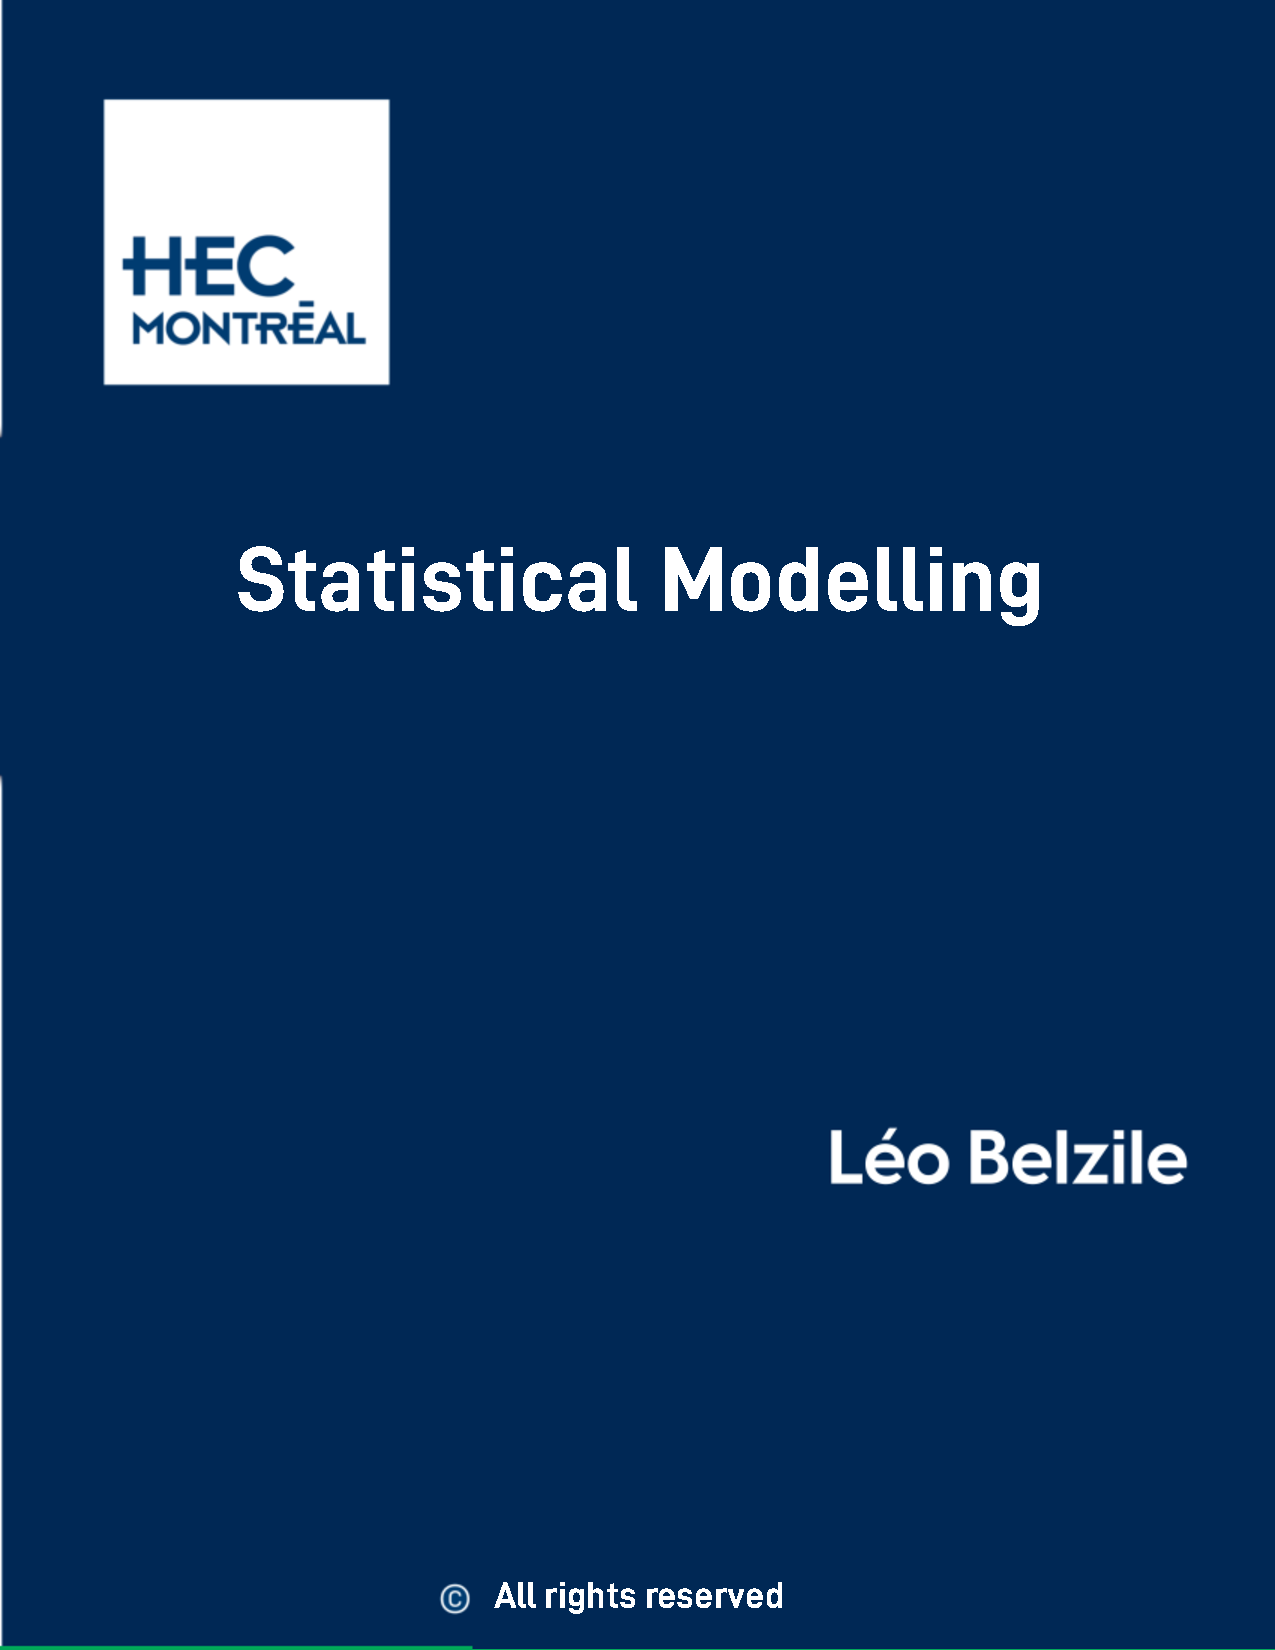
\includepdf{images/coverpage.pdf}

\renewcommand*\contentsname{Table of contents}
{
\setcounter{tocdepth}{2}
\tableofcontents
}

\mainmatter
\bookmarksetup{startatroot}

\chapter*{Welcome}\label{welcome}
\addcontentsline{toc}{chapter}{Welcome}

\markboth{Welcome}{Welcome}

These notes by Léo Belzile (HEC Montréal) are licensed under a
\href{http://creativecommons.org/licenses/by-nc-sa/4.0/}{Creative
Commons Attribution-NonCommercial-ShareAlike 4.0 International License}.

This course is about statistical modelling.

A famous quote attributed to George Box claims that

\begin{quote}
All models are wrong, but some are useful.
\end{quote}

This standpoint is reductive: Peter McCullagh and John Nelder wrote in
the preamble of their book (emphasis mine)

\begin{quote}
Modelling in science remains, partly at least, an art. Some principles
do exist, however, to guide the modeller. The first is that all models
are wrong; \textbf{some, though, are better} than others and we can
\textbf{search for the better ones}. At the same time we must recognize
that eternal truth is not within our grasp.
\end{quote}

And this quote by David R. Cox adds to the point:

\begin{quote}
\ldots it does not seem helpful just to say that all models are wrong.
The very word model implies simplification and idealization. The idea
that complex physical, biological or sociological systems can be exactly
described by a few formulae is patently absurd. The construction of
idealized representations that \textbf{capture important stable aspects
of such systems} is, however, a vital part of general scientific
analysis and statistical models, especially substantive ones, do not
seem essentially different from other kinds of model.
\end{quote}

Why use models?
\href{https://krugman.blogs.nytimes.com/2010/11/18/debt-deleveraging-and-the-liquidity-trap/}{Paul
Krugman wrote in 2010 in his blog}

\begin{quote}
The answer I'd give is that models are an enormously important tool for
clarifying your thought. You don't have to literally believe your model
--- in fact, you're a fool if you do --- to believe that putting
together a simplified but complete account of how things work, with all
the eyes crossed and teas dotted or something, helps you gain a much
more sophisticated understanding of the real situation. People who don't
use models end up relying on slogans that are much more simplistic than
the models
\end{quote}

\section*{Course content}\label{course-content}
\addcontentsline{toc}{section}{Course content}

\markright{Course content}

There are two main data type: \textbf{experimental} data are typically
collected in a control environment following a research protocol with a
particular experimental design: they serve to answer questions specified
ahead of time. This approach is highly desirable to avoid the garden of
forking paths
\href{http://www.stat.columbia.edu/~gelman/research/unpublished/p_hacking.pdf}{(researchers
unfortunately tend to refine or change their hypothesis in light of
data, which invalidates their findings} --- preregistration alleviates
this somewhat). While experimental data are highly desirable, it is not
always possible to collect experimental data: for example, an economist
cannot modify interest rates to see how it impacts consumer savings.
When data have been collected beforehand without intervention (for other
purposes), these are called \textbf{observational}. These will be the
ones most frequently encountered.

A stochastic model will comprise two ingredients: a distribution for the
random data and a formula linking the parameters or the conditional
expectation of a response variable \(Y\) to a set of explanatories
\(\mathbf{X}\). A model can serve to either predict new outcomes
(predictive modelling) or else to test research hypothesis about the
effect of the explanatory variables on the response (explanatory model).
These two objectives are of course not mutually exclusive even if we
distinguish in practice inference and prediction.

A predictive model gives predictions of \(Y\) for different combinations
of explanatory variables or future data. For example, one could try to
forecast the enery consumption of a house as a function of weather, the
number of inhabitants and its size. Black boxes used in machine learning
are often used solely for prediction: these models are not easily
interpreted and they often ignore the data structure.

By constrast, explicative models are often simple and interpretable:
regression models are often used for inference purpose and we will focus
on these. The following examples will be covered in class or as part of
the exercices:

\begin{itemize}
\tightlist
\item
  Are sequential decisions in online shop (buying or not, then selecting
  the quantity) preferable to integrated decisions
  (\citeproc{ref-Duke.Amir:2023}{Duke and Amir 2023})?
\item
  Determining what is the most distracting for road users: talking on a
  cellphone, texting or checking your smartwatch
  (\citeproc{ref-Brodeur:2021}{Brodeur et al. 2021})?
\item
  What is the impact of inconsistencies between product description and
  the displayed image (\citeproc{ref-Lee.Choi:2019}{Lee and Choi 2019})?
\item
  Is the price of gasoline more expensive in the Gaspé peninsula than in
  the rest of Quebec?
  \href{https://ici.radio-canada.ca/nouvelle/1463520/prix-essence-gaspesie-rapport-regie-energie}{A
  report of the \emph{Régie de l'énergie} examines the question}
\item
  Are driving tests in the UK easier if you live in a rural area?
  \href{https://www.theguardian.com/world/2019/aug/23/an-easy-ride-scottish-village-fuels-debate-driving-test-pass-rates}{An
  analysis of \emph{The Guardian}} hints that it is the case.
\item
  What is the environmental perception of a package that includes
  cardboard over a plastic container
  (\citeproc{ref-Sokolova:2023}{Sokolova, Krishna, and Döring 2023})?
\item
  What is the psychological impact of suggested amounts on donations
  (\citeproc{ref-Moon.VanEpps:2023}{Moon and VanEpps 2023})?
\item
  What are the benefits of face-to-face meetings, rather than via
  videoconference tools? Brucks and Levav
  (\citeproc{ref-Brucks.Levav:2022}{2022}) suggests a decrease in the
  number of creative ideas and interactions when meeting online.
\end{itemize}

\bookmarksetup{startatroot}

\chapter{Introduction}\label{intro}

This chapter reviews some basic notions of probability and statistics
that are normally covered in undergraduate or college.

\section{Population and samples}\label{population-sample}

Statistics is the science of uncertainty quantification: of paramount
importance is the notion of randomness. Generally, we will seek to
estimate characteristics of a population using only a sample (a
sub-group of the population of smaller size).

The \textbf{population of interest} is a collection of individuals which
the study targets. For example, the Labour Force Survey (LFS) is a
monthly study conducted by Statistics Canada, who define the target
population as ``all members of the selected household who are 15 years
old and older, whether they work or not.'' Asking every Canadian meeting
this definition would be costly and the process would be long: the
characteristic of interest (employment) is also a snapshot in time and
can vary when the person leaves a job, enters the job market or become
unemployed.

In general, we therefore consider only \textbf{samples} to gather the
information we seek to obtain. The purpose of \textbf{statistical
inference} is to draw conclusions about the population, but using only a
share of the latter and accounting for sources of variability. George
Gallup made this great analogy between sample and population:

\begin{quote}
One spoonful can reflect the taste of the whole pot, if the soup is
well-stirred
\end{quote}

A \textbf{sample} is a random sub-group of individuals drawn from the
population. Creation of sampling plans is a complex subject and
semester-long sampling courses would be required to evens scratch the
surface of the topic. Even if we won't be collecting data, keep in mind
the following information: for a sample to be good, it must be
representative of the population under study. Selection bias must be
avoided, notably samples of friends or of people sharing opinions.

Because the individuals are selected at \textbf{random} to be part of
the sample, the measurement of the characteristic of interest will also
be random and change from one sample to the next. However, larger
samples of the same quality carry more information and our estimator
will be more precise. Sample size is not guarantee of quality, as the
following example demonstrates.

\begin{example}[Polling for the 1936 USA Presidential
Election]\protect\hypertarget{exm-Galluppoll}{}\label{exm-Galluppoll}

\emph{The Literary Digest} surveyed 10 millions people by mail to know
voting preferences for the 1936 USA Presidential Election. A sizeable
share, 2.4 millions answered, giving Alf Landon (57\%) over incumbent
President Franklin D. Roosevelt (43\%). The latter nevertheless won in a
landslide election with 62\% of votes cast, a 19\% forecast error.
\href{https://www.jstor.org/stable/2749114}{Biased sampling and
differential non-response are mostly responsible for the error:} the
sampling frame was built using ``phone number directories, drivers'
registrations, club memberships, etc.'', all of which skewed the sample
towards rich upper class white people more susceptible to vote for the
GOP.

In contrast, Gallup correctly predicted the outcome by polling (only)
50K inhabitants.
\href{https://ozanozbey.medium.com/two-lessons-of-sampling-bias-from-1936-us-election-e4e96bd42be}{Read
the full story here.}

\end{example}

\subsection{Variable type}\label{variable-type}

\begin{itemize}
\tightlist
\item
  a \textbf{variable} represents a characteristic of the population, for
  example the sex of an individual, the price of an item, etc.
\item
  an \textbf{observation} is a set of measures (variables) collected
  under identical conditions for an individual or at a given time.
\end{itemize}

\begin{longtable}[]{@{}
  >{\raggedleft\arraybackslash}p{(\columnwidth - 12\tabcolsep) * \real{0.0923}}
  >{\raggedright\arraybackslash}p{(\columnwidth - 12\tabcolsep) * \real{0.1231}}
  >{\raggedright\arraybackslash}p{(\columnwidth - 12\tabcolsep) * \real{0.1692}}
  >{\raggedright\arraybackslash}p{(\columnwidth - 12\tabcolsep) * \real{0.1385}}
  >{\raggedright\arraybackslash}p{(\columnwidth - 12\tabcolsep) * \real{0.2615}}
  >{\raggedleft\arraybackslash}p{(\columnwidth - 12\tabcolsep) * \real{0.1385}}
  >{\raggedright\arraybackslash}p{(\columnwidth - 12\tabcolsep) * \real{0.0769}}@{}}

\caption{\label{tbl-data-renfe}First lines of the \texttt{renfe}
database, which contains the price of 10K train tickets between Madrid
and Barcelona. The columns \texttt{price} and \texttt{duration}
represent continuous variables, all others are categorical.}

\tabularnewline

\toprule\noalign{}
\begin{minipage}[b]{\linewidth}\raggedleft
price
\end{minipage} & \begin{minipage}[b]{\linewidth}\raggedright
type
\end{minipage} & \begin{minipage}[b]{\linewidth}\raggedright
class
\end{minipage} & \begin{minipage}[b]{\linewidth}\raggedright
fare
\end{minipage} & \begin{minipage}[b]{\linewidth}\raggedright
dest
\end{minipage} & \begin{minipage}[b]{\linewidth}\raggedleft
duration
\end{minipage} & \begin{minipage}[b]{\linewidth}\raggedright
wday
\end{minipage} \\
\midrule\noalign{}
\endhead
\bottomrule\noalign{}
\endlastfoot
143.4 & AVE & Preferente & Promo & Barcelona-Madrid & 190 & 6 \\
181.5 & AVE & Preferente & Flexible & Barcelona-Madrid & 190 & 2 \\
86.8 & AVE & Preferente & Promo & Barcelona-Madrid & 165 & 7 \\
86.8 & AVE & Preferente & Promo & Barcelona-Madrid & 190 & 7 \\
69.0 & AVE-TGV & Preferente & Promo & Barcelona-Madrid & 175 & 4 \\

\end{longtable}

The choice of statistical model and test depends on the underlying type
of the data collected. There are many choices: quantitative (discrete or
continuous) if the variables are numeric, or qualitative (binary,
nominal, ordinal) if they can be described using an adjective; I prefer
the term categorical, which is more evocative.

Most of the models we will deal with are so-called regression models, in
which the mean of a quantitative variable is a function of other
variables, termed explanatories. There are two types of numerical
variables

\begin{itemize}
\tightlist
\item
  a discrete variable takes a finite or countable number of values,
  prime examples being binary variables or count variables.
\item
  a continuous variable can take (in theory) an infinite possible number
  of values, even when measurements are rounded or measured with a
  limited precision (time, width, mass). In many case, we could also
  consider discrete variables as continuous if they take enough values
  (e.g., money).
\end{itemize}

Categorical variables take only a finite of values. They are regrouped
in two groups,

\begin{itemize}
\tightlist
\item
  nominal if there is no ordering between levels (sex, color, country of
  origin) or
\item
  ordinal if they are ordered (Likert scale, salary scale) and this
  ordering should be reflected in graphs or tables.
\end{itemize}

We will bundle every categorical variable using arbitrary encoding for
the levels: for modelling, these variables taking \(K\) possible values
(or levels) must be transformed into a set of \(K-1\) binary 0/1
variables, the omitted level corresponding to a baseline. Failing to
declare categorical variables in your favorite software is a common
mistake, especially when these are saved in the database using integers
rather than strings.

\section{Random variable}\label{random-variable}

Suppose we wish to describe the behaviour of a stochastic phenomenon. To
this effect, one should enumerate the set of possible values taken by
the variable of interest and their probability: this is what is encoded
in the distribution.

Random variables are denoted using capital letters: for example
\(Y \sim \mathsf{normal}(\mu, \sigma^2)\) indicates that \(Y\) follows a
normal distribution with parameters \(\mu\) and \(\sigma>0.\) If the
values of the latter are left unspecified, we talk about the family of
distributions. When the values are given, for example \(\mu=0\) and
\(\sigma=1\), we deal with a single distribution for which a function
encode the probability of the underlying variable.

\begin{definition}[Distribution function, mass function and
density]\protect\hypertarget{def-cdf}{}\label{def-cdf}

The (cumulative) distribution function \(F(y)\) gives the cumulative
probability that an event doesn't exceed a given numerical value \(y\),
\(F(y) = \mathsf{Pr}(Y \leq y).\)

If \(Y\) is discrete, then it has atoms of non-zero probability and we
call \(f\) the mass function, and \(f(y)=\mathsf{Pr}(Y=y)\) gives the
probability of each outcome \(y.\) In the continuous case, no numerical
value has non-zero probability and so we consider intervals instead. The
density function \(f(x)\) is non-negative and satisfies
\(\int_{\mathbb{R}} f(x) \mathrm{d}x=1\): the integral over a set \(B\)
(the area under the curve) gives the probability of \(Y\) falling inside
\(B \in \mathbb{R}.\) It follows that the distribution function of a
continuous random variable is simply
\(F(y) = \int_{-\infty}^y f(x) \mathrm{d} x.\)

\begin{figure}[ht!]

{\centering 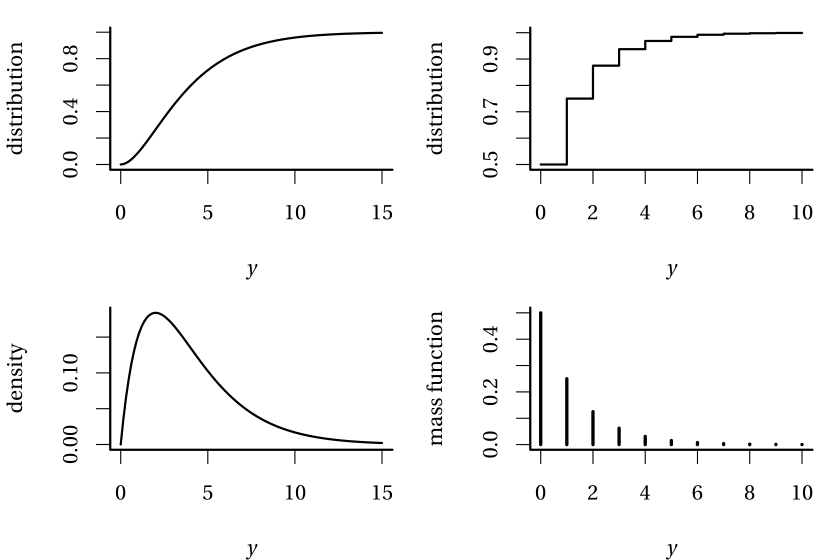
\includegraphics[width=0.85\textwidth,height=\textheight]{images/02-ttest-DF_illustration.png}

}

\caption{(Cumulative) distribution functions (top) and density/mass
functions (bottom) of continuous (left) and discrete (right) random
variables.}

\end{figure}%

\end{definition}

One of the first topics covered in introductory statistics is
descriptive statistics such as the mean and standard deviation. These
are estimators of (centered) moments, which characterise a random
variable. In the case of the standard normal distribution, the
expectation and variance fully characterize the distribution.

\begin{definition}[Moments]\protect\hypertarget{def-moments}{}\label{def-moments}

Let \(Y\) be a random variable with density (or mass) function \(f(x).\)
The \textbf{expectation} (or theoretical mean) of a continuous random
variable \(Y\) is \begin{align*}
\mathsf{E}(Y)=\int_{\mathbb{R}} x f(x) \mathrm{d} x.
\end{align*} In the discrete case, we set rather
\(\mu = \mathsf{E}(Y)=\sum_{x \in \mathcal{X}} x \mathsf{Pr}(X=x)\),
where \(\mathcal{X}\) denotes the support of \(Y\), the set of numerical
values at which the probability of \(Y\) is non-zero. More generally, we
can look at the expectation of a function \(g(x)\) for \(Y\), which is
nothing but the integral (or sum in the discrete case) of \(g(x)\)
weighted by the density or mass function of \(f(x).\) In the same
fashion, provided the integral is finite, the variance is \begin{align*}
\mathsf{Va}(Y)=\mathsf{E}\{Y-\mathsf{E}(Y)\}^2 \equiv \int_{\mathbb{R}} (x-\mu)^2 f(x) \mathrm{d} x.
\end{align*} The \textbf{standard deviation} is the square root of the
variance, \(\mathsf{sd}(Y)=\sqrt{\mathsf{Va}(Y)}\): it units are the
same as those of \(Y\) and are thus more easily interpreted.

The notion of moments can be extended to higher dimensions. Consider an
\(n\)-vector \(\boldsymbol{Y}.\) In the regression setting, the response
\(\boldsymbol{Y}\) would usually comprise repeated measures on an
individual, or even observations from a group of individuals.

The expected value (theoretical mean) of the vector \(\boldsymbol{Y}\)
is calculated componentwise, i.e., \begin{align*}
\mathsf{E}(\boldsymbol{Y}) &= \boldsymbol{\mu}=
\begin{pmatrix}
\mathsf{E}(Y_1) &
\cdots  &
\mathsf{E}(Y_n)
\end{pmatrix}^\top
\end{align*} whereas the second moment of \(\boldsymbol{Y}\) is encoded
in the \(n \times n\) \textbf{covariance} matrix \begin{align*}
\mathsf{Va}(\boldsymbol{Y}) &= \boldsymbol{\Sigma} = \begin{pmatrix} \mathsf{Va}(Y_1) & \mathsf{Co}(Y_1, Y_2)  & \cdots & \mathsf{Co}(Y_1, Y_n) \\
\mathsf{Co}(Y_2, Y_1) & \mathsf{Va}(Y_2) & \ddots & \vdots \\
\vdots & \ddots & \ddots & \vdots \\
\mathsf{Co}(Y_n, Y_1) & \mathsf{Co}(Y_n, Y_2) &\cdots & \mathsf{Va}(Y_n)
\end{pmatrix}
\end{align*} The \(i\)th diagonal element of \(\boldsymbol{\Sigma}\),
\(\sigma_{ii}=\sigma_i^2\), is the variance of \(Y_i\), whereas the
off-diagonal entries \(\sigma_{ij}=\sigma_{ji}\) \((i \neq j)\) are the
covariance of pairwise entries, with \begin{align*}
\mathsf{Co}(Y_i, Y_j) = \int_{\mathbb{R}^2} (y_i-\mu_i)(y_j-\mu_j) f_{Y_i, Y_j}(y_i, y_j) \mathrm{d} y_i \mathrm{d} y_j.
\end{align*} The covariance matrix \(\boldsymbol{\Sigma}\) is thus
symmetric. It is customary to normalize the pairwise dependence so they
do not depend on the component variance. The linear \textbf{correlation}
between \(Y_i\) and \(Y_j\) is \begin{align*}
\rho_{ij}=\mathsf{Cor}(Y_i,Y_j)=\frac{\mathsf{Co}(Y_i, Y_j)}{\sqrt{\mathsf{Va}(Y_i)}\sqrt{\mathsf{Va}(Y_j)}}=\frac{\sigma_{ij}}{\sigma_i\sigma_j}.
\end{align*} The correlation matrix of \(\boldsymbol{Y}\) is an
\(n\times n\) symmetric matrix with ones on the diagonal and the
pairwise correlations off the diagonal, \begin{align*}
\mathsf{Cor}(\boldsymbol{Y})=
\begin{pmatrix}
1 & \rho_{12} & \rho_{13} & \cdots & \rho_{1n}\\
\rho_{21} & 1 & \rho_{23} & \cdots & \rho_{2n} \\
\rho_{31} & \rho_{32} & 1 & \ddots & \rho_{3n} \\
\vdots & \vdots & \ddots & \ddots & \vdots \\
\rho_{n1} & \rho_{n2} & \rho_{n3} & \cdots & 1
\end{pmatrix}.
\end{align*} One of the most important parts of modelling correlated (or
longitudinal) data is the need to account for within-group correlations.
This basically comes down to modelling a covariance matrix for
observations within the same group (or within the same individual in the
case of repeated measures), which is the object of
\href{correlated-longitudinal-data}{Chapter 5}.

\end{definition}

\begin{definition}[Bias]\protect\hypertarget{def-bias}{}\label{def-bias}

The bias of an estimator \(\hat{\theta}\) for a parameter \(\theta\) is
\begin{align*}
 \mathsf{bias}(\hat{\theta})=\mathsf{E}(\hat{\theta})- \theta
 \end{align*} The estimator is unbiased if its bias is zero.

\end{definition}

\begin{example}[Unbiased
estimators]\protect\hypertarget{exm-unbiased-estimator}{}\label{exm-unbiased-estimator}

The unbiased estimator of the mean and the variance of \(Y\) are
\begin{align*}
\overline{Y}_n &= n^{-1} \sum_{i=1}^n Y_i\\
S_n &= (n-1)^{-1} \sum_{i=1}^n (Y_i-\overline{Y})^2.
\end{align*}

\end{example}

While unbiasedness is a desirable property, there may be cases where no
unbiased estimator exists for a parameter! Often, rather, we seek to
balance bias and variance: recall that an estimator is a function of
random variables and thus it is itself random: even if it is unbiased,
the numerical value obtained will vary from one sample to the next.

\begin{definition}[]\protect\hypertarget{def-mse}{}\label{def-mse}

We often seek an estimator that minimises the \textbf{mean squared
error}, \begin{align*}
\mathsf{MSE}(\hat{\theta}) = \mathsf{E}\{(\hat{\theta}-\theta)^2\}=\mathsf{Va}(\hat{\theta}) + \{\mathsf{E}(\hat{\theta})\}^2.
\end{align*} The mean squared error is an objective function consisting
of the sum of the squared bias and the variance.

\end{definition}

Most estimators we will considered are so-called maximum likelihood
estimator. These estimator are asymptotically efficient, in the sense
that they have the lowest mean squared error of all estimators for large
samples. Other properties of maximum likelihood estimators also make
them attractive default choice for estimation.

\section{Discrete distributions}\label{discrete-distributions}

Many distributions for discrete random variables have a simple empirical
justification, stemming from simple combinatorial arguments (counting).
We revisit the most common ones.

\begin{definition}[Bernoulli
distribution]\protect\hypertarget{def-bernoullidist}{}\label{def-bernoullidist}

We consider a binary event such as coin toss (heads/tails). In general,
the two events are associated with success/failure. By convention,
failures are denoted by zeros and successes by ones, the probability of
success being \(p\) so \(\mathsf{Pr}(Y=1)=p\) and
\(\mathsf{Pr}(Y=0)=1-p\) (complementary event). The mass function of the
\href{https://en.wikipedia.org/wiki/Bernoulli_distribution}{Bernoulli
distribution} is thus \begin{align*}
\mathsf{Pr}(Y=y) = p^y (1-p)^{1-y}, \quad y=0, 1.
\end{align*}

\end{definition}

A rapid calculation shows that \(\mathsf{E}(Y)=p\) and
\(\mathsf{Va}(Y)=p(1-p).\) Indeed, \begin{align*}
\mathsf{E}(Y) = \mathsf{E}(Y^2) = p \cdot 1 + (1-p) \cdot 0 = p.
\end{align*}

Many research questions have binary responses, for example:

\begin{itemize}
\tightlist
\item
  did a potential client respond favourably to a promotional offer?
\item
  is the client satisfied with service provided post-purchase?
\item
  will a company go bankrupt in the next three years?
\item
  did a study participant successfully complete a task?
\end{itemize}

Oftentimes, we will have access to aggregated data.

\begin{definition}[Binomial
distribution]\protect\hypertarget{def-binomialdist}{}\label{def-binomialdist}

If we consider the sum of independent and identically distributed
Bernoulli events, the number of sucesses \(Y\) out of \(m\) trials is
\href{https://en.wikipedia.org/wiki/Binomial_distribution}{binomial},
denoted \(\mathsf{Bin}(m, p)\); the mass function of the binomial
distribution is \begin{align*}
\mathsf{Pr}(Y=y) = \binom{m}{y}p^y (1-p)^{1-y}, \quad y=0, 1.
\end{align*} The likelihood of a sample from a binomial distribution is
(up to a normalizing constant that doesn't depend on \(p\)) the same as
that of \(m\) independent Bernoulli trials. The expectation of the
binomial random variable is \(\mathsf{E}(Y)=mp\) and its variance
\(\mathsf{Va}(Y)=mp(1-p).\)

\end{definition}

As examples, we could consider the number of successful candidates out
of \(m\) who passed their driving license test or the number of
customers out of \(m\) total which spent more than 10\$ in a store.

More generally, we can also consider count variables whose realizations
are integer-valued, for examples the number of

\begin{itemize}
\tightlist
\item
  insurance claims made by a policyholder over a year,
\item
  purchases made by a client over a month on a website,
\item
  tasks completed by a study participant in a given time frame.
\end{itemize}

\begin{definition}[Poisson
distribution]\protect\hypertarget{def-poissondist}{}\label{def-poissondist}

If the probability of success \(p\) of a Bernoulli event is small in the
sense that \(mp \to \lambda\) when the number of trials \(m\) increases,
then the number of success follows approximately a Poisson distribution
with mass function \begin{align*}
\mathsf{Pr}(Y=y) = \frac{\exp(-\lambda)\lambda^y}{\Gamma(y+1)}, \quad y=0, 1, 2, \ldots
\end{align*} where \(\Gamma(\cdot)\) denotes the gamma function. The
parameter \(\lambda\) of the Poisson distribution is both the
expectation and the variance of the distribution, meaning
\(\mathsf{E}(Y)=\mathsf{Va}(Y)=\lambda.\)

\end{definition}

\begin{definition}[Negative binomial
distribution]\protect\hypertarget{def-negbindist}{}\label{def-negbindist}

The negative binomial distribution arises if we consider the number of
Bernoulli trials with probability of success \(p\) until we obtain \(m\)
success. Let \(Y\) denote the number of failures: the order of success
and failure doesn't matter, except for the latest trial which must be a
success. The mass function of the negative binomial is \begin{align*}
\mathsf{Pr}(Y=y)= \binom{m-1+y}{y} p^m (1-p)^{y}.
\end{align*}

The negative binomial distribution also appears as the unconditional
distribution of a two-stage hierarchical gamma-Poisson model, in which
the mean of the Poisson distribution is random and follows a gamma
distribution. In notation, this is
\(Y \mid \Lambda=\lambda \sim \mathsf{Po}(\lambda)\) and \(\Lambda\)
follows a gamma distribution with shape \(r\) and scale \(\theta\),
whose density is \begin{align*}
f(x) = \theta^{-r}x^{r-1}\exp(-x/\theta)/\Gamma(r).
\end{align*} The unconditional number of success is then negative
binomial.

In the context of generalized linear models, we will employ yet another
parametrisation of the distribution, with the mass function
\begin{align*}
\mathsf{Pr}(Y=y)=\frac{\Gamma(y+r)}{\Gamma(y+1)\Gamma(r)} \left(\frac{r}{r + \mu} \right)^{r} \left(\frac{\mu}{r+\mu}\right)^y, y=0, 1, \ldots, \mu,r >0,
\end{align*} where \(\Gamma\) is the gamma function and the parameter
\(r>0\) is not anymore integer valued. The expectation and variance of
\(Y\) are \(\mathsf{E}(Y)=\mu\) et \(\mathsf{Va}(Y)=\mu+k\mu^2\), where
\(k=1/r.\) The variance of the negative binomial distribution is thus
higher than its expectation, which justifies the use of the negative
binomial distribution for modelling overdispersion.

\end{definition}

\section{Continuous distributions}\label{continuous-distributions}

We will encounter many continuous distributions that arise as
(asymptotic) null distribution of test statistics because of the central
limit theorem, or that follow from transformation of Gaussian random
variables.

\begin{definition}[Beta
distribution]\protect\hypertarget{def-loibeta}{}\label{def-loibeta}

The beta distribution \(\mathsf{Beta}(\alpha, \beta)\) is a distribution
supported on the unit interval \([0,1]\) with shape parameters
\(\alpha>0\) and \(\beta>0.\) It's density is \begin{align*}
f(x) = \frac{\Gamma(\alpha)\Gamma(\beta)}{\Gamma(\alpha+\beta)}x^{\alpha-1}(1-x)^{1-\beta}, \qquad x \in [0,1].
\end{align*} The case \(\alpha=\beta=1\), also denoted
\(\mathsf{unif}(0,1)\), corresponds to a standard uniform distribution.

\begin{figure}[ht!]

\centering{

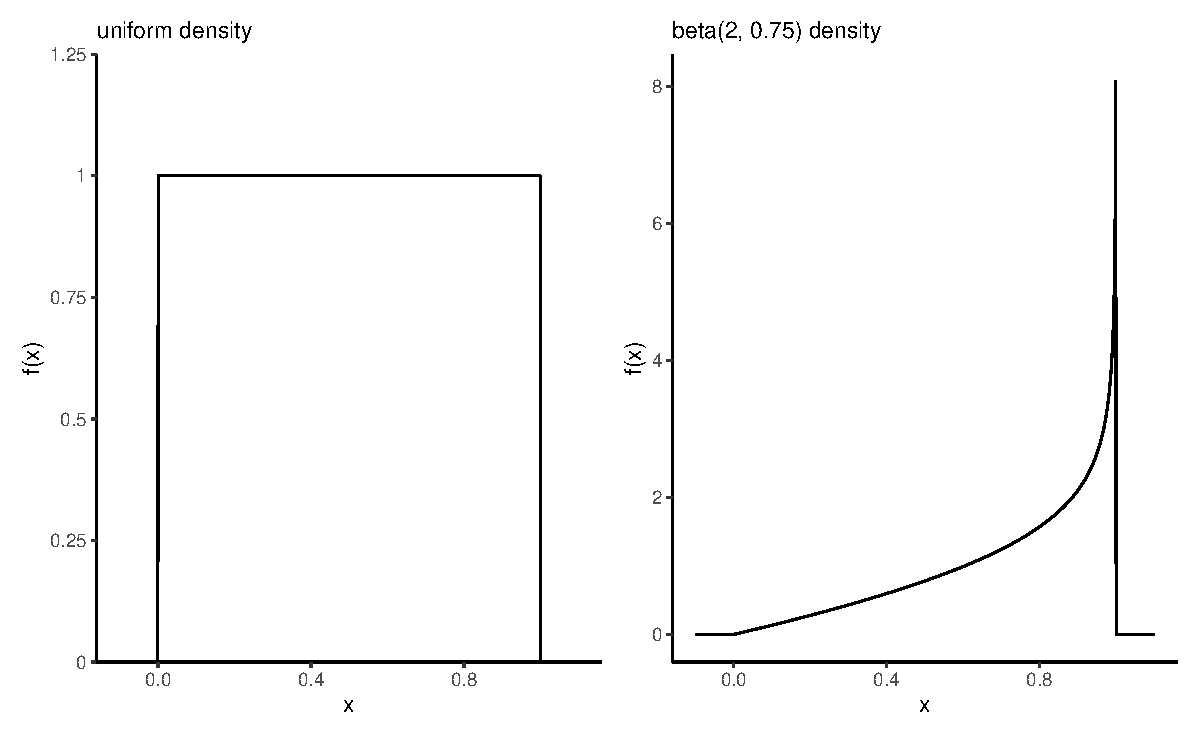
\includegraphics[width=0.85\textwidth,height=\textheight]{introduction_files/figure-pdf/fig-densite-beta-1.pdf}

}

\caption{\label{fig-densite-beta}Density fonction of uniform (left) and
beta(2, 3/4) random variables on the unit interval.}

\end{figure}%

\end{definition}

\begin{definition}[Exponential
distribution]\protect\hypertarget{def-exponentialdist}{}\label{def-exponentialdist}

The exponential distribution plays a prominent role in the study of
waiting time of Poisson processes, and in survival analysis. One
caracteristic of the distribution is it's absence of memory:
\(\Pr(Y \geq y + u \mid Y > u) = \Pr(Y > u)\) for \(y, u>0.\)

The distribution function of the exponential distribution with scale
\(\lambda>0\), denoted \(Y \sim \mathsf{Exp}(\lambda)\), is
\(F(x) = 1-\exp(-x/\lambda)\) and the corresponding density function is
\(f(x) =\lambda^{-1}\exp(-x/\lambda)\) for \(x >0.\) The expected value
of \(Y\) is simply \(\lambda.\)

\end{definition}

\begin{definition}[Normal
distribution]\protect\hypertarget{def-normaldist}{}\label{def-normaldist}

Ths most well known distribution, the normal distribution is ubiquitous
in statistics because of the central limit theorem (CLT), which
describes the behaviour of the sample mean in large sample.The
parameters \(\mu\) and \(\sigma>0\) that fully characterize the
distribution of the normal distribution and they correspond to the
expectation and standard deviation. The density of a normal distribution
is symmetric around \(\mu\), while \(\sigma\) describes the dispersion
around this mode. The bell-shaped density function is \begin{align*}
f(x) = (2\pi\sigma^2)^{-1/2} \exp \left\{ - \frac{(x-\mu)^2}{2\sigma^2}\right\}, \qquad x \in \mathbb{R}.
\end{align*}

\begin{figure}[ht!]

\centering{

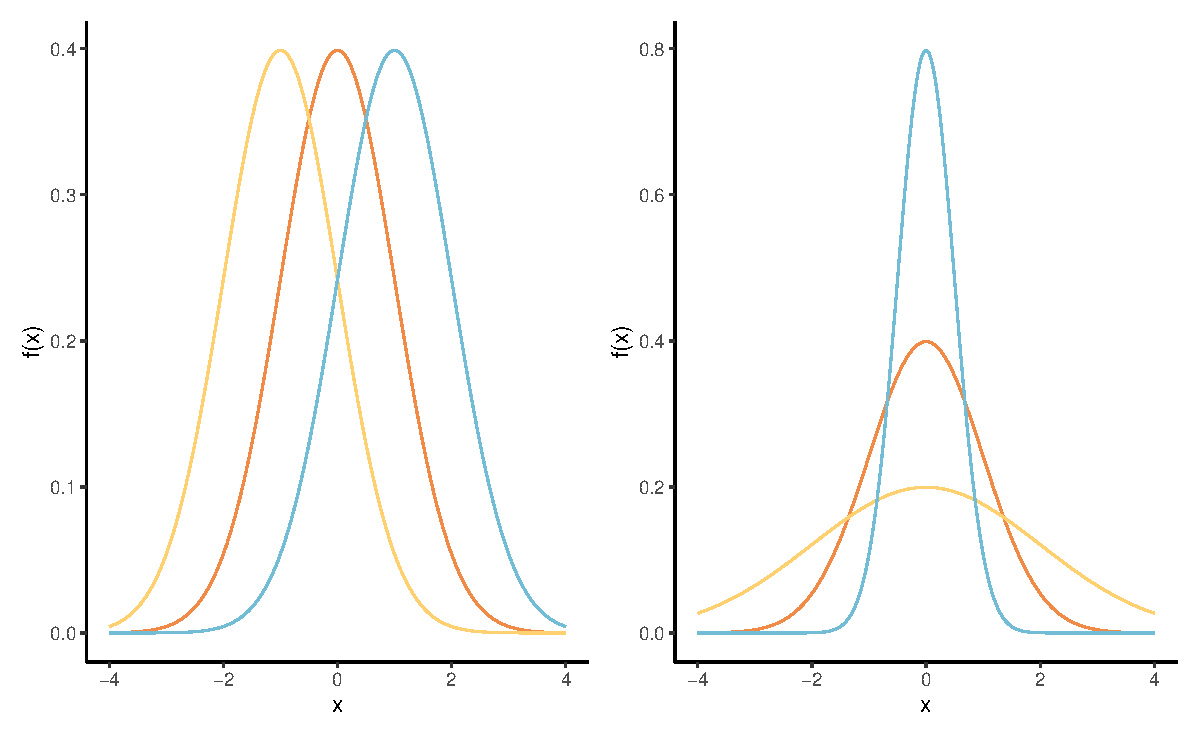
\includegraphics[width=0.85\textwidth,height=\textheight]{introduction_files/figure-pdf/fig-normal-loc-scale-1.pdf}

}

\caption{\label{fig-normal-loc-scale}Densities of normal distributions
with different mean parameters (left) and different scale parameters
(right).}

\end{figure}%

The distribution function of the normal distribution is not available in
closed-form. The normal distribution is a location-scale distribution:
if \(Y \sim \mathsf{normal}(\mu, \sigma^2)\), then
\(Z = (Y-\mu)/\sigma \sim \mathsf{normale}(0,1).\) Conversely, if
\(Z \sim \mathsf{normal}(0,1)\), then
\(Y = \mu + \sigma Z \sim \mathsf{normal}(\mu, \sigma^2).\)

We will also encounter the multivariate normal distribution; for a \(d\)
dimensional vector
\(\boldsymbol{Y} \sim \mathsf{normal}_d(\boldsymbol{\mu}, \boldsymbol{\Sigma})\),
the density is \begin{align*}
f(\boldsymbol{x}) = (2\pi)^{-d/2} |\boldsymbol{\Sigma}|^{-1/2} \exp \left\{ - \frac{1}{2} (\boldsymbol{x}-\boldsymbol{\mu})^\top \boldsymbol{\Sigma}^{-1}(\boldsymbol{x}-\boldsymbol{\mu})\right\}
\end{align*}

The mean vector \(\boldsymbol{\mu}\) is the vector of expectation of
individual observations, whereas \(\boldsymbol{\Sigma}\) is the
\(d \times d\) covariance matrix of \(\boldsymbol{Y}.\) A unique
property of the multivariate normal distribution is the link between
independence and the covariance matrix: if \(Y_i\) and \(Y_j\) are
independent, the \((i,j)\) off-diagonal entry of \(\boldsymbol{\Sigma}\)
is zero.

\end{definition}

\begin{definition}[Chi-square
distribution]\protect\hypertarget{def-chisquare-dist}{}\label{def-chisquare-dist}

The chi-square distribution with \(\nu>0\) degrees of freedom, denoted
\(\chi^2_\nu\) or \(\mathsf{chi-square}(\nu).\) It's density is
\begin{align*}
f(x; \nu) = \frac{1}{2^{\nu/2}\Gamma(\nu/2)}x^{\nu/2-1}\exp(-x/2),\qquad x >0.
\end{align*} It can be obtained for \(\nu\) integer by considering the
following: if we consider \(k\) independent and identically distributed
standard normal variables, \(Y_i \sim \mathsf{normal}(0, 1)\), then
\(\sum_{i=1}^k Y_i^2\) follows a chi-square distribution with \(k\)
degrees of freedom, denote \(\chi^2_k.\) The square of a standard normal
variate likewise follows a \(\chi^2_1\) distribution. The expectation of
\(\chi^2_k\) random variable is \(k.\)

\end{definition}

If we consider a sample of \(n\) normally distributed observations, the
scaled sample variance \((n-1)S^2/\sigma^2 \sim \chi^2_{n-1}.\)

\begin{definition}[Student-\(t\)
distribution]\protect\hypertarget{def-studentdist}{}\label{def-studentdist}

The Student-\(t\) distribution with \(\nu>0\) degrees of freedom is a
location-scale family. The standard version is denoted by
\(\mathsf{Student}(\nu).\)

The name ``Student'' comes from the pseudonym used by William Gosset in
Gosset (\citeproc{ref-Student:1908}{1908}), who introduced the
asymptotic distribution of the \(t\)-statistic. The density of the
standard \(T\) with \(\nu\) degrees of freedom is \begin{align*}
f(y; \nu) = \frac{\Gamma \left( \frac{\nu+1}{2}\right)}{\Gamma\left(\frac{\nu}{2}\right)
\sqrt{\nu\pi}}\left(1+\frac{y^{2}}{\nu}\right)^{-\frac{\nu+1}{2}}
\end{align*} the distribution has polynomial tails, is symmetric around
\(0\) and unimodal. As \(\nu \to \infty\), the Student distribution
converges to a normal distribution. It has heavier tails than the normal
distribution and only the first \(\nu-1\) moments of the distribution
exist, so a Student distribution with \(\nu=2\) degrees of freedom has
infinite variance.

For normally distributed data, the centered sample mean divided by the
sample variance, \((\overline{Y}-\mu)/S^2\) follows a Student-\(t\)
distribution with \(n-1\) degrees of freedom, which explains the
terminology \(t\)-tests.

\begin{figure}[ht!]

\centering{

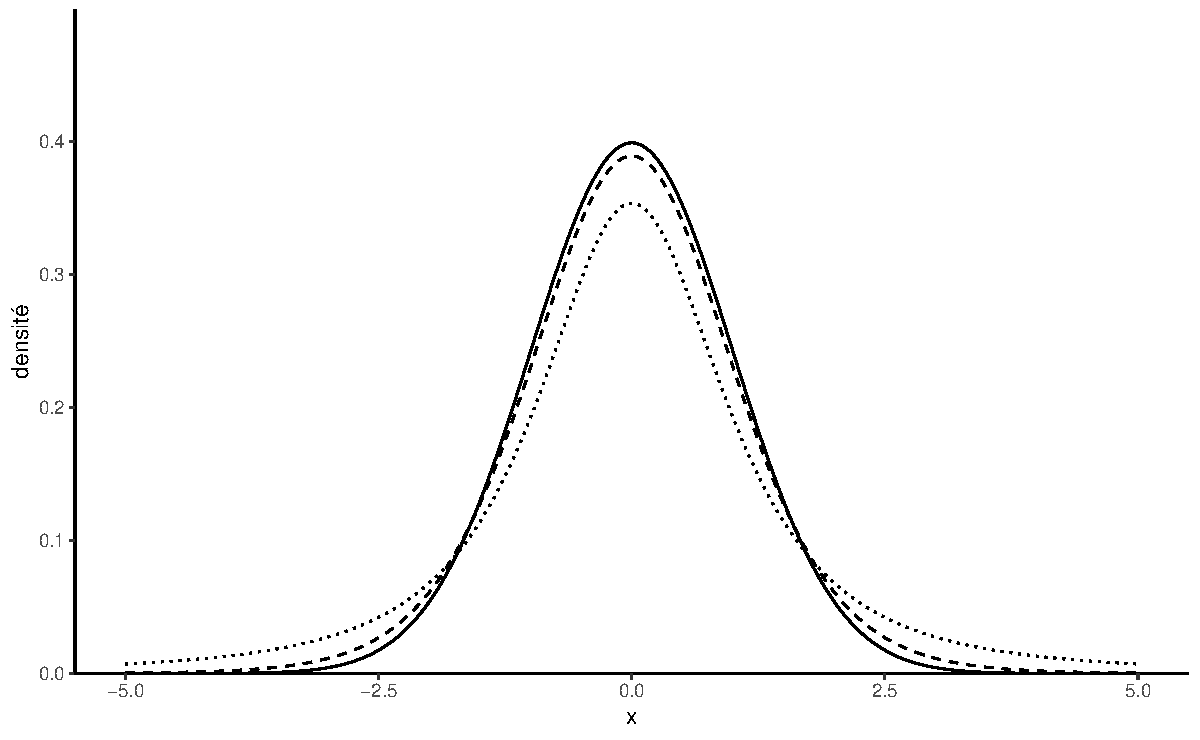
\includegraphics[width=0.5\textwidth,height=\textheight]{introduction_files/figure-pdf/fig-student-density-1.pdf}

}

\caption{\label{fig-student-density}Comparison between the Student-\(t\)
density for varying degrees of freedom, with \(\nu=2\) (dotted),
\(\nu=10\) (dashed) and the normal density (\(\nu = \infty).\)}

\end{figure}%

\end{definition}

\begin{definition}[Fisher
distribution]\protect\hypertarget{def-Fdist}{}\label{def-Fdist}

The Fisher or \(F\) distribution is used to determine the large sample
behaviour of test statistics for comparing different group averages (in
analysis of variance) assuming data are normally distributed.

The \(F\) distribution, denoted \(\mathsf{Fisher}(\nu_1, \nu_2)\), is
obtained by dividing two independent chi-square random variables with
respective degrees of freedom \(\nu_1\) and \(\nu_2.\) Specifically, if
\(Y_1 \sim \chi^2_{\nu_1}\) and \(Y_2 \sim \chi^2_{\nu_2}\), then
\begin{align*}
F = \frac{Y_1/\nu_1}{Y_2/\nu_2} \sim \mathsf{Fisher}(\nu_1, \nu_2)
\end{align*}

The Fisher distribution tends to a \(\chi^2_{\nu_1}\) when
\(\nu_2 \to \infty.\)

\end{definition}

\section{Graphs}\label{graphs}

This section reviews the main graphical representation of random
variables, depending on their type.

The main type of graph for representing categorical variables is bar
plot (and modifications thereof). In a bar plot, the frequency of each
category is represented in the \(y\)-axis as a function of the (ordered)
levels on the \(x\)-axis. This representation is superior to the
\href{http://www.perceptualedge.com/articles/08-21-07.pdf}{ignominious
pie chart}, a nuisance that ought to be banned (humans are very bad at
comparing areas and a simple rotation changes the perception of the
graph)!

\begin{figure}[ht!]

\centering{

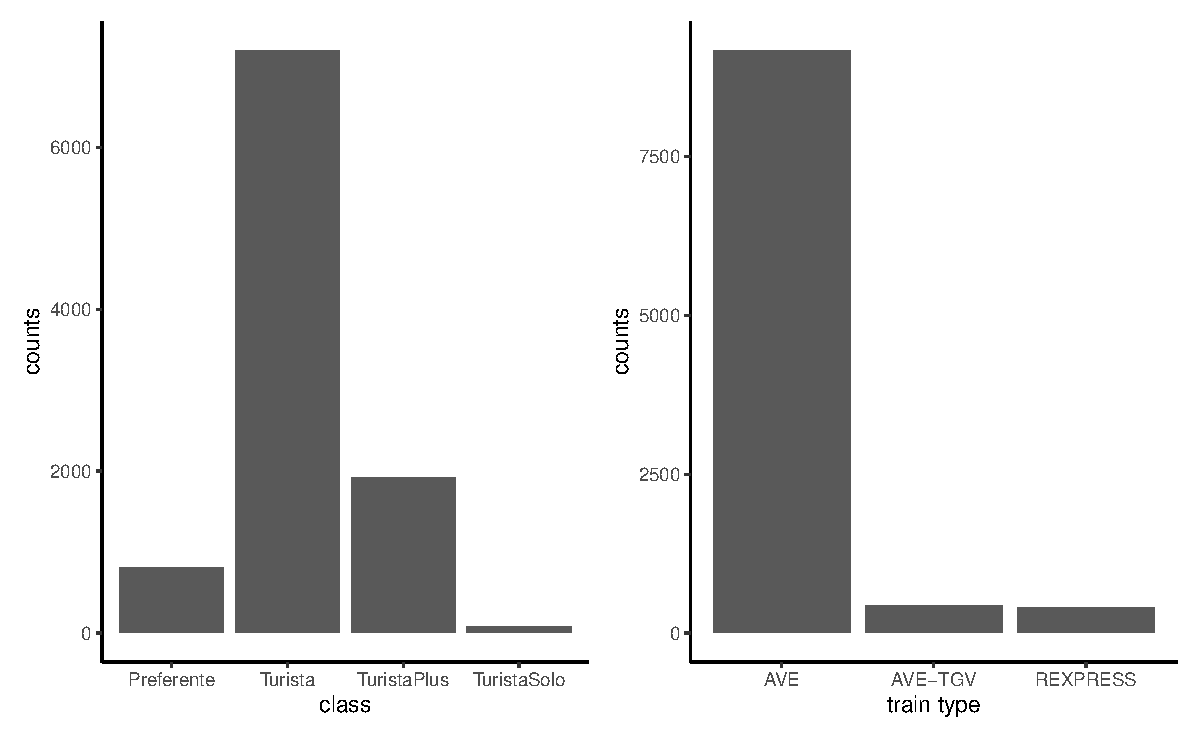
\includegraphics[width=0.85\textwidth,height=\textheight]{introduction_files/figure-pdf/fig-barplotrenfe-1.pdf}

}

\caption{\label{fig-barplotrenfe}Bar plot of ticket class for Renfe
tickets data}

\end{figure}%

Continuous variables can take as many distinct values as there are
observations, so we cannot simply count the number of occurences by
unique values. Instead, we bin them into distinct intervals so as to
obtain an histogram. The number of class depends on the number of
observations: as a rule of thumb, the number of bins should not exceed
\(\sqrt{n}\), where \(n\) is the sample size. We can then obtain the
frequency in each class, or else normalize the histogram so that the
area under the bands equals one: this yields a discrete approximation of
the underlying density function. Varying the number of bins can help us
detect patterns (rounding, asymmetry, multimodality).

Since we bin observations together, it is sometimes difficult to see
where they fall. Adding rugs below or above the histogram will add
observation about the range and values taken, where the heights of the
bars in the histogram carry information about the (relative) frequency
of the intervals.

\begin{figure}[ht!]

\centering{

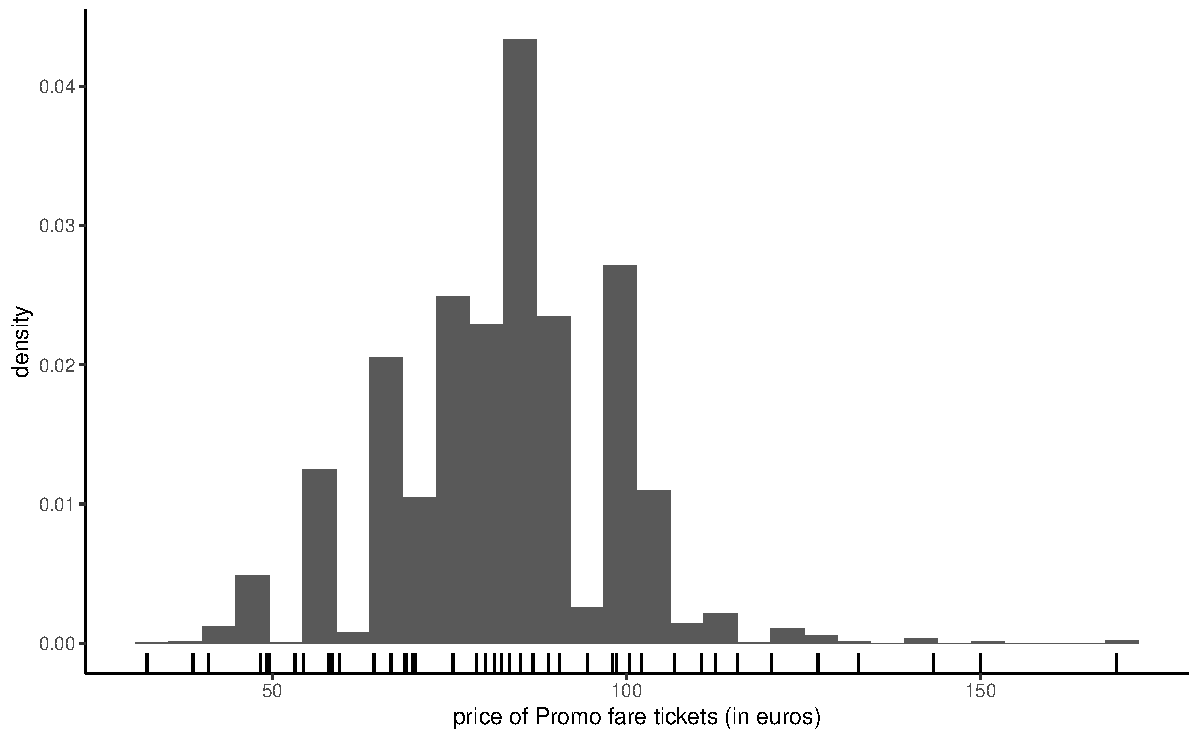
\includegraphics[width=0.85\textwidth,height=\textheight]{introduction_files/figure-pdf/fig-histrenfe-1.pdf}

}

\caption{\label{fig-histrenfe}Histogram of Promo tickets for Renfe
ticket data}

\end{figure}%

If we have a lot of data, it sometimes help to focus only on selected
summary statistics.

\begin{definition}[Box-and-whiskers
plot]\protect\hypertarget{def-boxplot}{}\label{def-boxplot}

A box-and-whiskers plot (or boxplot) represents five numbers

\begin{itemize}
\tightlist
\item
  The box gives the quartiles \(q_1, q_2, q_3\) of the distribution. The
  middle bar \(q_2\) is thus the median, so 50\% of the observations are
  smaller or larger than this number.
\item
  The length of the whiskers is up to \(1.5\) times the interquartiles
  range \(q_3-q_1\) (the whiskers extend until the latest point in the
  interval, so the largest observation that is smaller than
  \(q_3+1.5(q_3-q_1)\), etc.)
\item
  Observations beyond the whiskers are represented by dots or circles,
  sometimes termed outliers. However, beware of this terminology: the
  larger the sample size, the more values will fall outside the
  whiskers. This is a drawback of boxplots, which was conceived at a
  time where the size of data sets was much smaller than what is current
  standards.
\end{itemize}

\begin{figure}[ht!]

\centering{

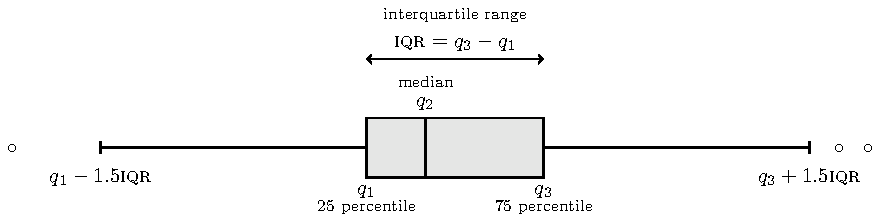
\includegraphics[width=0.85\textwidth,height=\textheight]{images/01-intro-boxplot.pdf}

}

\caption{\label{fig-boxplot}Box-and-whiskers plot}

\end{figure}%

\end{definition}

We can represent the distribution of a response variable as a function
of a categorical variable by drawing a boxplot for each category and
laying them side by side. A third variable, categorical, can be added
via a color palette, as shown in Figure~\ref{fig-histboxplot}.

\begin{figure}[ht!]

\centering{

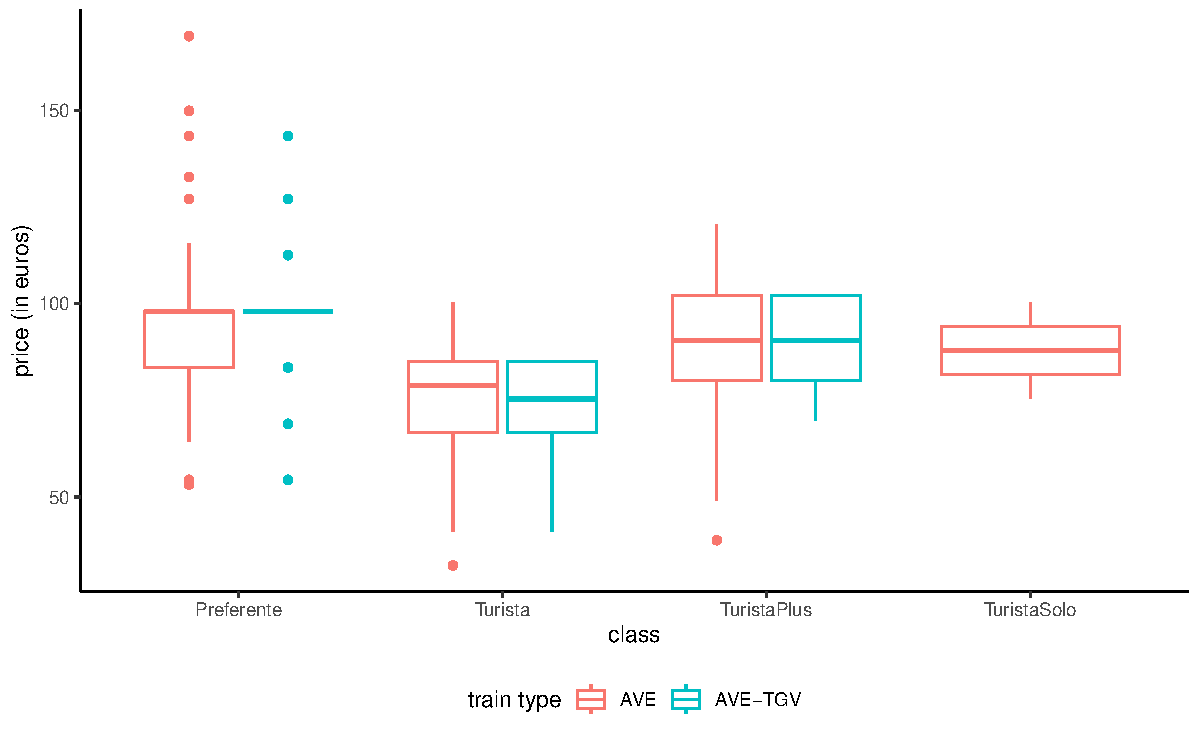
\includegraphics[width=0.85\textwidth,height=\textheight]{introduction_files/figure-pdf/fig-histboxplot-1.pdf}

}

\caption{\label{fig-histboxplot}Box-and-whiskers plots for Promo fare
tickets as a function of class and type for the Renfe tickets data.}

\end{figure}%

Scatterplots are used to represent graphically the co-variation between
two continuous variables: each tuple gives the coordinate of the point.
If only a handful of large values are visible on the graph, a
transformation may be useful: oftentimes, you will encounter graphs
where the \(x\)- or \(y\)-axis is on the log-scale when the underlying
variable is positive. If the number of data points is too large, it is
hard to distinguish points because they are overlaid: adding
transparency, or binning using a two-dimensional histogram with the
frequency represented using color are potential solutions. The left
panel of Figure~\ref{fig-scatterplot} shows the 100 simulated
observations, whereas the right-panel shows a larger sample of 10 000
points using hexagonal binning, an analog of the bivariate density.

\begin{figure}[ht!]

\centering{

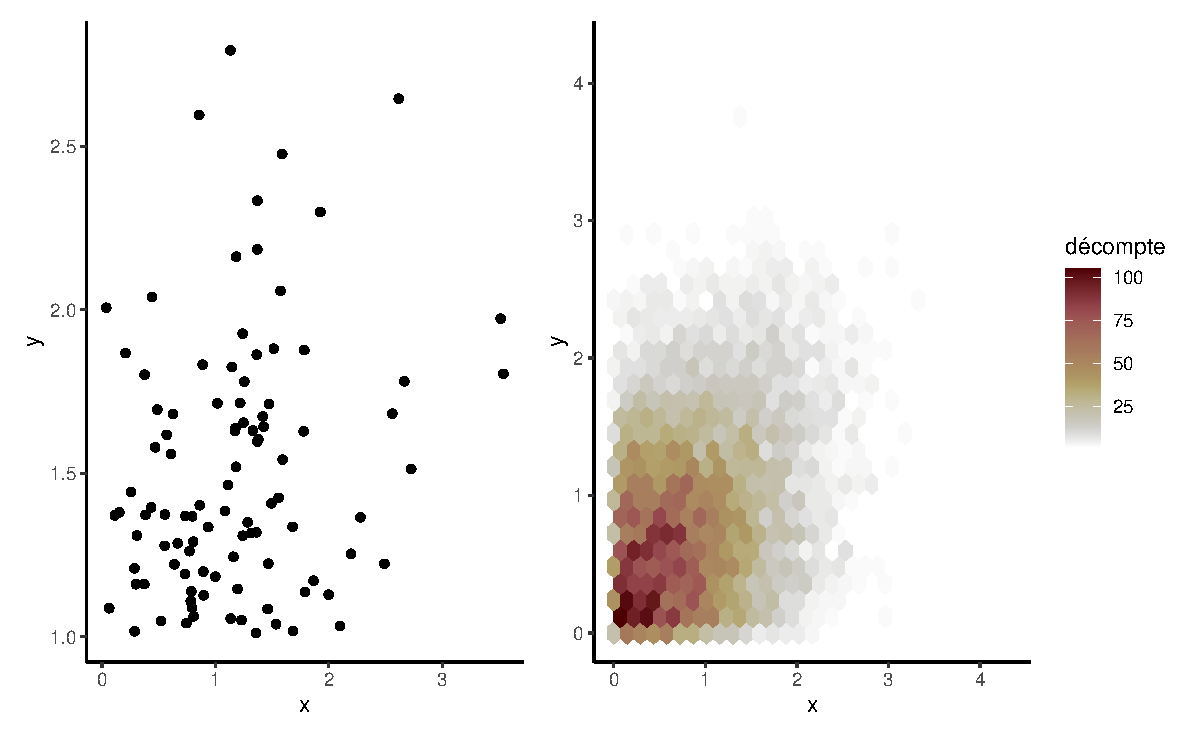
\includegraphics[width=0.85\textwidth,height=\textheight]{introduction_files/figure-pdf/fig-scatterplot-1.pdf}

}

\caption{\label{fig-scatterplot}Scatterplot (left) and hexagonal heatmap
of bidimensional bin counts (right) of simulated data.}

\end{figure}%

Models are (at best) an approximation of the true data generating
mechanism and we will want to ensure that our assumptions are reasonable
and the quality of the fit decent.

\begin{definition}[Quantiles-quantiles
plots]\protect\hypertarget{def-qqplot}{}\label{def-qqplot}

Quantile-quantile plots are graphical goodness-of-fit diagnostics that
are based on the following principle: if \(Y\) is a continuous random
variable with distribution function \(F\), then the mapping
\(F(Y) \sim \mathsf{unif}(0,1)\) yields standard uniform variables.
Similarly, the quantile transform applied to a uniform variable provides
a mean to simulating samples from \(F\), viz.~\(F^{-1}(U).\) Consider
then a random sample of size \(n\) from the uniform distribution ordered
from smallest to largest, with \(U_{(1)} \leq \cdots \leq U_{(n)}.\) One
can show these ranks have marginally a Beta distribution,
\(U_{(k)} \sim \mathsf{beta}(k, n+1-k)\) with expectation \(k/(n+1).\)

In practice, we don't know \(F\) and, even if we did, one would need to
estimate the parameters. We consider some estimator \(\widehat{F}\) for
the model and apply the inverse transform to an approximate uniform
sample \(\{i/(n+1)\}_{i=1}^n.\) The quantile-quantile plot shows the
data as a function of the (first moment) of the transformed order
statistics:

\begin{itemize}
\tightlist
\item
  on the \(x\)-axis, the theoretical quantiles
  \(\widehat{F}^{-1}\{\mathrm{rank}(y_i)/(n+1)\}\)
\item
  on the \(y\)-axis, the empirical quantiles \(y_i\)
\end{itemize}

If the model is adequate, the ordered values should follow a straight
line with unit slope passing through the origin.

\end{definition}

\begin{figure}[ht!]

\centering{

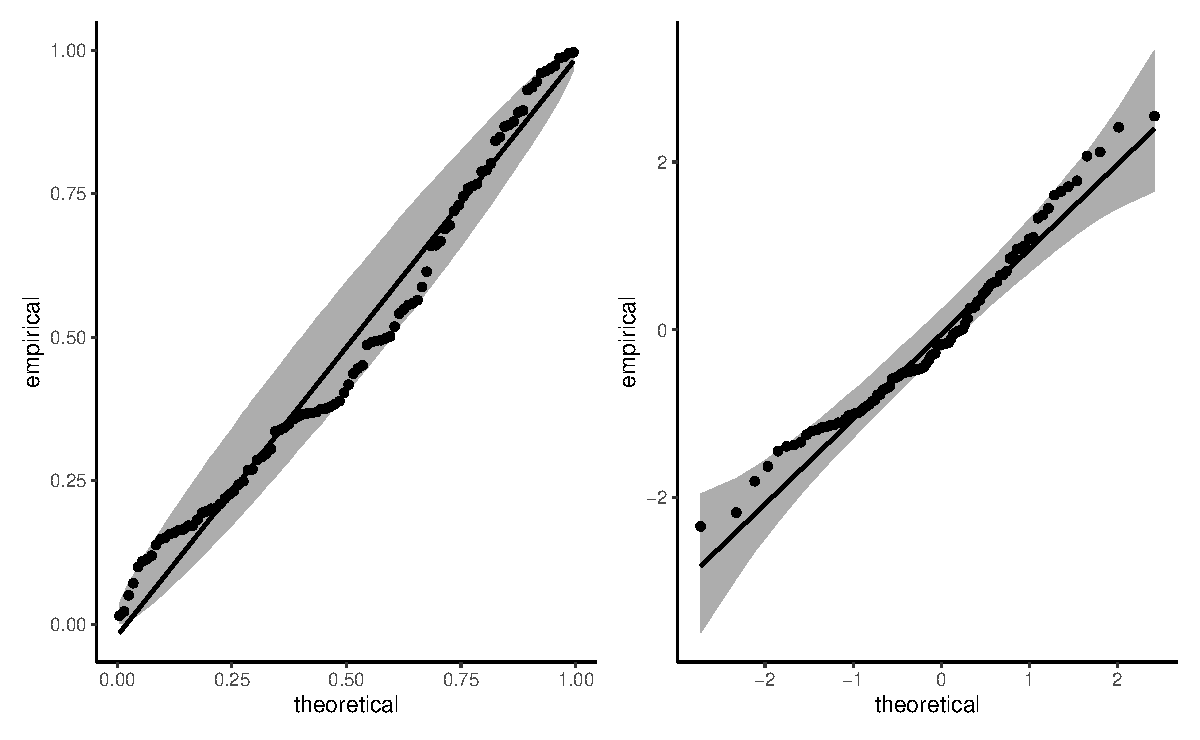
\includegraphics[width=0.85\textwidth,height=\textheight]{introduction_files/figure-pdf/fig-diagrammeqq2-1.pdf}

}

\caption{\label{fig-diagrammeqq2}Probability-probability plot (left) on
uniform margins, and ormal quantile-quantile plot (right) for the same
dataset.}

\end{figure}%

Even if we knew the true distribution of the data, the sample
variability makes it very difficult to spot if deviations from the model
are abnormal or compatible with the model. A simple point estimate with
no uncertainty measure can lead to wrong conclusions. As such, we add
approximate pointwise or simultaneous confidence intervals. The simplest
way to do this is by simulation, by repeating the following steps \(B\)
times:

\begin{enumerate}
\def\labelenumi{\arabic{enumi}.}
\tightlist
\item
  simulate a sample \(\{Y^{(b)}_{i}\} (i=1,\ldots, n)\) from
  \(\widehat{F}\)
\item
  re-estimate the parameters of \(F\) to obtain \(\widehat{F}_{(b)}\)
\item
  calculate and save the plotting positions
  \(\widehat{F}^{-1}_{(b)}\{i/(n+1)\}.\)
\end{enumerate}

The result of this operation is an \(n \times B\) matrix of simulated
data. We obtain a symmetric (\(1-\alpha\)) confidence interval by
keeping the empirical quantile of order \(\alpha/2\) and \(1-\alpha/2\)
from each row. The number \(B\) should be larger than 999, say, and be
chosen so that \(B/\alpha\) is an integer.

For the pointwise interval, each order statistic from the sample is a
statistic and so the probability of any single one falling outside the
confidence interval is approximately \(\alpha.\) However, order
statistics are not independent (they are ordered), so its common to see
neighbouring points falling outside of their respective intervals. The
intervals shown in Figure~\ref{fig-diagrammeqq2} are pointwise and
derived (magically) using a simple function. The uniform order
statistics have larger variability as we move away from 0.5, but the
uncertainty in the quantile-quantile plot largely depends on \(F.\)

Interpretation of quantile-quantile plots requires practice and
experience:
\href{https://stats.stackexchange.com/questions/101274/how-to-interpret-a-qq-plot/101290\#101290}{this
post by \emph{Glen\_b} on StackOverflow} nicely summarizes what can be
detected (or not) from them.

\section{Laws of large numbers}\label{law-large-numbers}

An estimator for a parameter \(\theta\) is \textbf{consistent} if the
value obtained as the sample size increases (to infinity) converges to
the true value of \(\theta.\) Mathematically speaking, this translates
into convergence in probability, meaning
\(\hat{\theta} \stackrel{\mathsf{Pr}}{\to} \theta.\) In common language,
we say that the probability that \(\hat{\theta}\) and \(\theta\) differ
becomes negligible as \(n\) gets large.

Consistency is the \emph{a minima} requirement for an estimator: when we
collect more information, we should approach the truth. The law of large
number states that the sample mean of \(n\) (independent) observations
with common mean \(\mu\), say \(\overline{Y}_n\), converges to \(\mu\),
denoted \(\overline{Y}_n \rightarrow \mu.\) Roughly speaking, our
approximation becomes less variable and asymptotically unbiased as the
sample size (and thus the quantity of information available for the
parameter) increases. The law of large number is featured in Monte Carlo
experiments: we can approximate the expectation of some (complicated)
function \(g(x)\) by simulating repeatedly independent draws from \(Y\)
and calculating the sample mean \(n^{-1} \sum_{i=1}^n g(Y_i).\)

If the law of large number tells us what happens in the limit (we get a
single numerical value), the result doesn't contain information about
the rate of convergence and the uncertainty at finite levels.

\section{Central Limit Theorem}\label{CLT}

The central limit theorem gives the approximate large sample
distribution of the sample mean. Consider a random sample of size \(n\)
\(\{Y_i\}_{i=1}^n\) of independent random variables with common
expectation \(\mu\) and variance \(\sigma^2.\) The sample mean
\(\overline{Y} = n^{-1}\sum_{i=1}^n Y_i\) converges to \(\mu\) by the
law of large number, but we also have that

\begin{itemize}
\tightlist
\item
  the estimator \(\overline{Y}\) is centered around \(\mu\),
\item
  the standard error is \(\sigma/\sqrt{n}\); the rate of convergence is
  thus \(\sqrt{n}.\) For a sample of size 100, the standard error of the
  sample mean will be 10 times smaller than that of the underlying
  random variable.
\item
  the sample mean, once properly scaled, follows approximately a normal
  distribution
\end{itemize}

Mathematically, the central limit theorem states
\(\sqrt{n}(\overline{Y}-\mu) \stackrel{\mathrm{d}}{\rightarrow} \mathsf{normal}(0, \sigma^2).\)
If \(n\) is large (a rule of thumb is \(n>30\), but this depends on the
underlying distribution of \(Y\)), then
\(\overline{Y} \stackrel{\cdot}{\sim} \mathsf{normal}(\mu, \sigma^2/n).\)

How do we make sense of this result? Let us consider the mean travel
time of high speed Spanish trains (AVE) between Madrid and Barcelona
that are operated by Renfe.

\begin{figure}[ht!]

\centering{

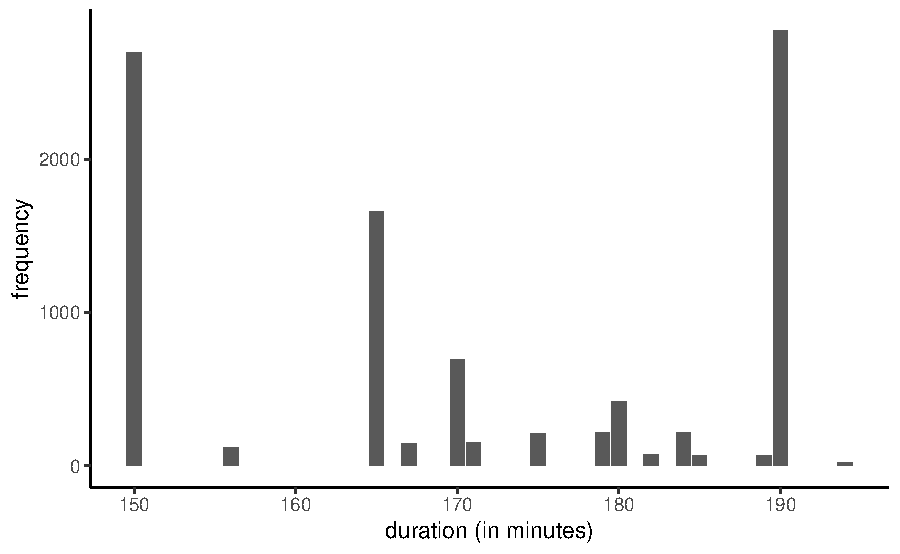
\includegraphics[width=0.85\textwidth,height=\textheight]{introduction_files/figure-pdf/fig-renfeclt-1.pdf}

}

\caption{\label{fig-renfeclt}Empirical distribution of travel times of
high speed trains.}

\end{figure}%

Our exploratory data analysis showed previously that the duration is the
one advertised on the ticket: there are only 15 unique travel time.
Based on 9603 observations, we estimate the mean travel time to be 170
minutes and 41 seconds. Figure~\ref{fig-renfeclt} shows the empirical
distribution of the data.

Consider now samples of size \(n=10\), drawn repeatedly from the
population: in the first sample, the sample mean is 169.3 minutes,
whereas we get an estimate of 167 minutes in our second , 157.9 minutes
in the third, etc.

\begin{figure}[ht!]

\centering{

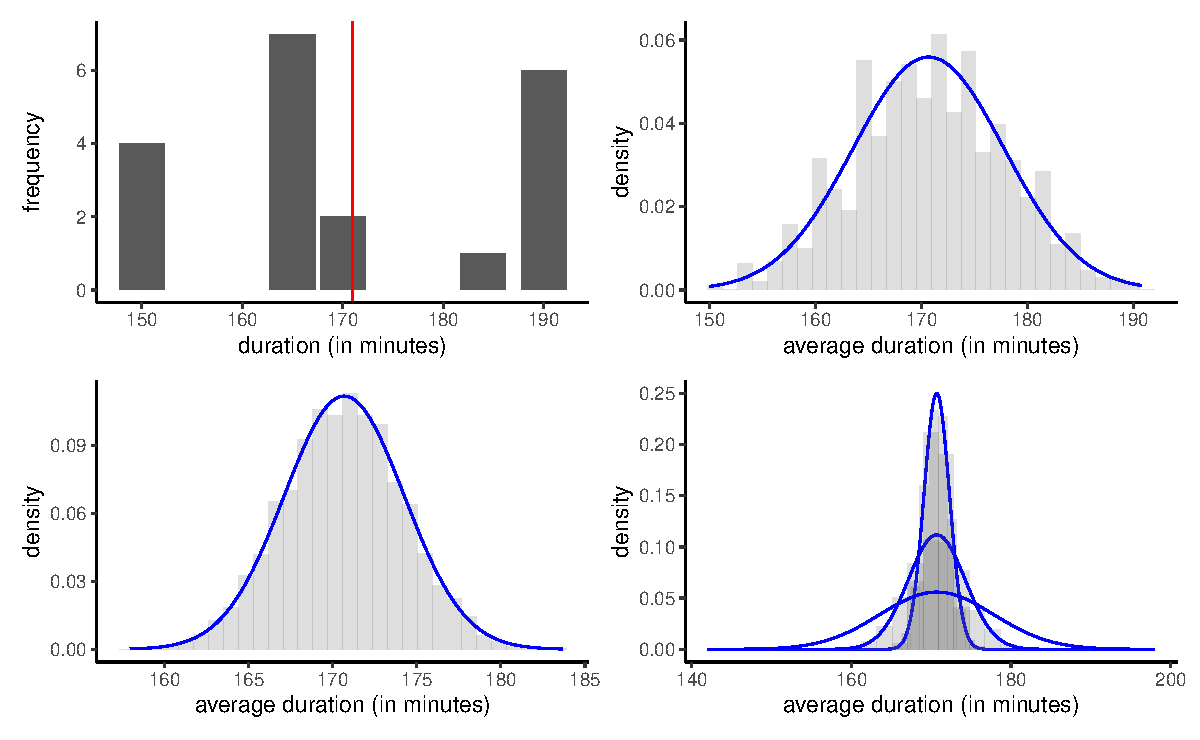
\includegraphics[width=0.9\textwidth,height=\textheight]{introduction_files/figure-pdf/fig-renfemeanCLT-1.pdf}

}

\caption{\label{fig-renfemeanCLT}Graphical representation of the central
limit theorem. The upper left panel shows a sample of 20 observations
with its sample mean (vertical red). The three other panels show the
histograms of the sample mean from repeated samples of size 5 (top
right), 20 (bottom left) and 20, 50 and 100 overlaid, with the density
approximation provided by the central limit theorem.}

\end{figure}%

We draw \(B=1000\) different samples, each of size \(n=5\), from two
millions records, and calculate the sample mean in each of them. The top
right panel of Figure~\ref{fig-renfemeanCLT} is a histogram of the
sample means when \(n=5\), whereas the bottom left panel shows the same
thingfor \(n=20.\) The last graph of Figure~\ref{fig-renfemeanCLT} shows
the impact of the increase in sample size: whereas the normal
approximation is okay-ish for \(n=5\), it is indistinguishable from the
normal approximation for \(n=20.\) As \(n\) increases and the sample
size gets bigger, the quality of the approximation improves and the
curve becomes more concentrated around the true mean. Even if the
distribution of the travel time is discrete, the mean is approximately
normal.

We considered a single distribution in the example, but you could play
with other distributions and vary the sample size to see when the
central limit theorem kicks in usng this
\href{http://195.134.76.37/applets/AppletCentralLimit/Appl_CentralLimit2.html}{applet}.

The central limit theorem underlies why scaled test statistics which
have sample mean zero and sample variance 1 have a standard null
distribution in large sample: this is what guarantees the validity of
our inference!

\bookmarksetup{startatroot}

\chapter{Statistical inference}\label{inference}

In most applied domains, empirical evidences drive the advancement of
the field and data from well designed experiments contribute to the
built up of science. In order to draw conclusions in favour or against a
theory, researchers turn (often unwillingly) to statistics to back up
their claims. This has led to the prevalence of the use of the null
hypothesis statistical testing (NHST) framework. One important aspect of
the reproducibility crisis is the misuse of \(p\)-values in journal
articles: falsification of a null hypothesis is not enough to provide
substantive findings for a theory.

Because introductory statistics course typically present hypothesis
tests without giving much thoughts to the underlying construction
principles of such procedures, users often have a reductive view of
statistics as a catalogue of pre-determined procedures. To make a
culinary analogy, users focus on learning recipes rather than trying to
understand the basics of cookery. This chapter focuses on understanding
of key ideas related to testing.

\begin{tcolorbox}[enhanced jigsaw, coltitle=black, colframe=quarto-callout-important-color-frame, breakable, opacityback=0, title=\textcolor{quarto-callout-important-color}{\faExclamation}\hspace{0.5em}{Important}, left=2mm, arc=.35mm, colbacktitle=quarto-callout-important-color!10!white, opacitybacktitle=0.6, titlerule=0mm, rightrule=.15mm, bottomtitle=1mm, toptitle=1mm, leftrule=.75mm, colback=white, toprule=.15mm, bottomrule=.15mm]

\textbf{Learning objectives}:

\begin{itemize}
\tightlist
\item
  Understanding the role of uncertainty in decision making.
\item
  Understanding the importance of signal-to-noise ratio as a measure of
  evidence.
\item
  Knowing the basic ingredients of hypothesis testing and being capable
  of correctly formulating and identifying these components in a paper.
\item
  Correctly interpreting \(p\)-values and confidence intervals for a
  parameter.
\end{itemize}

\end{tcolorbox}

The first step of a design is formulating a research question.
Generally, this hypothesis will specify potential differences between
population characteristics due to some intervention (a treatment) that
the researcher wants to quantify. This is the step during which
researchers decide on sample size, choice of response variable and
metric for the measurement, write down the study plan, etc.

It is important to note that most research questions cannot be answered
by simple tools. Researchers wishing to perform innovative
methodological research should contact experts and consult with
statisticians \textbf{before} they collect their data to get information
on how best to proceed for what they have in mind so as to avoid the
risk of making misleading and false claims based on incorrect analysis
or data collection.

\begin{figure}[ht!]

\centering{


\includegraphics[width=0.6\textwidth,height=\textheight]{images/xkcd2569_hypothesis_generation.png}

}

\caption{\label{fig-xkcd2569}xkcd comic
\href{https://xkcd.com/2569/}{2569 (Hypothesis generation) by Randall
Munroe}. Alt text: Frazzled scientists are requesting that everyone
please stop generating hypotheses for a little bit while they work
through the backlog. Cartoon reprinted under the
\href{https://creativecommons.org/licenses/by-nc/2.5/}{CC BY-NC 2.5
license}.}

\end{figure}%

\section{Sampling variability}\label{sampling-variability}

Given data, a researcher will be interested in estimating particular
characteristics of the population. We can characterize the set of all
potential values their measurements can take, together with their
frequency, via a distribution.

The purpose of this section is to illustrate how we cannot simply use
raw differences between groups to make meaningful comparisons: due to
sampling variability, samples will be alike even if they are generated
in the same way, but there will be always be differences between their
summary statistics. Such differences tend to attenuate (or increase) as
we collect more sample. Inherent to this is the fact that as we gather
more data (and thus more information) about our target, the portrait
becomes more precise. This is ultimately what allows us to draw
meaningful conclusions but, in order to do so, we need first to
determine what is likely or plausible and could be a stroke of luck, and
what is not likely to occur solely due to randomness.

We call numerical summaries of the data \textbf{statistics}. Its
important to distinguish between procedures/formulas and their numerical
values. An \textbf{estimator} is a rule or formula used to calculate an
estimate of some parameter or quantity of interest based on observed
data (like a recipe for cake). Once we have observed data we can
actually compute the sample mean, that is, we have an estimate --- an
actual value (the cake), which is a single realization and not random.
In other words,

\begin{itemize}
\tightlist
\item
  an estimand is our conceptual target, like the population
  characteristic of interest (population mean).
\item
  an estimator is the procedure or formula telling us how to transform
  the sample data into a numerical summary that is a proxy of our
  target.
\item
  an estimate is a number, the numerical value obtained once we apply
  the formula to observed data.
\end{itemize}

\begin{figure}[ht!]

\begin{minipage}{0.33\linewidth}

\centering{


\includegraphics[width=0.85\textwidth,height=\textheight]{images/estimand.jpg}

}

\subcaption{\label{fig-cake-1}Estimand}

\end{minipage}%
%
\begin{minipage}{0.33\linewidth}

\centering{

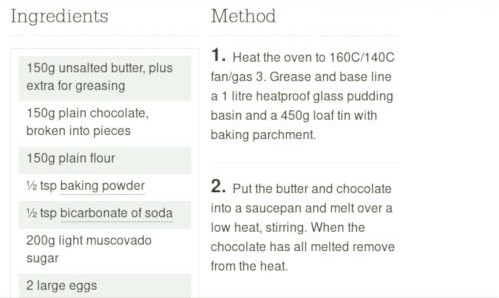
\includegraphics[width=0.85\textwidth,height=\textheight]{images/estimator.jpg}

}

\subcaption{\label{fig-cake-2}Estimator}

\end{minipage}%
%
\begin{minipage}{0.33\linewidth}

\centering{


\includegraphics[width=0.85\textwidth,height=\textheight]{images/estimate.jpg}

}

\subcaption{\label{fig-cake-3}Estimate}

\end{minipage}%

\caption{\label{fig-cake}\href{https://www.flickr.com/photos/darkdwarf/16563489881}{Estimand}
(left), estimator (middle) and
\href{https://www.flickr.com/photos/bensutherland/14685548773}{estimate}
(right) illustrated with cakes and based on an original idea of Simon
Grund. Cake photos shared under
\href{https://creativecommons.org/licenses/by-nc/2.0/}{CC BY-NC 2.0
license}.}

\end{figure}%

For example, we may use as estimand the population average of
\(Y_1, \ldots,\) say \(\mu.\) The estimator will be sample mean, i.e.,
the sum of the elements in the sample divided by the sample size,
\(\overline{Y}=(Y_1 + \cdots + Y_n)/n.\) The estimate will be a
numerical value, say 4.3.

Because the inputs of the estimator are random, the output is also
random and change from one sample to the next: even if you repeat a
recipe, you won't get the exact same result every time, as in
Figure~\ref{fig-xkcd605}.

\begin{figure}[ht!]

\centering{

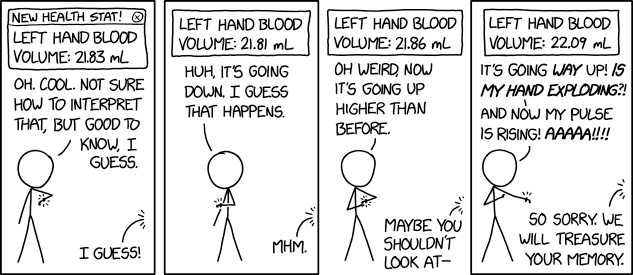
\includegraphics[width=0.7\textwidth,height=\textheight]{images/xkcd2581_health_stats.png}

}

\caption{\label{fig-xkcd605}xkcd comic
\href{https://xkcd.com/2581/}{2581 (Health Stats) by Randall Munroe}.
Alt text: You will live on forever in our hearts, pushing a little extra
blood toward our left hands now and then to give them a squeeze. Cartoon
reprinted under the
\href{https://creativecommons.org/licenses/by-nc/2.5/}{CC BY-NC 2.5
license}.}

\end{figure}%

To illustrate this point, Figure~\ref{fig-samplevar} shows five simple
random samples of size \(n=10\) drawn from an hypothetical population
with mean \(\mu\) and standard deviation \(\sigma,\) along with their
sample mean \(\overline{y}.\) Because of the sampling variability, the
sample means of the subgroups will differ even if they originate from
the same distribution. You can view sampling variability as noise: our
goal is to extract the signal (typically differences in means) but
accounting for spurious results due to the background noise.

\begin{figure}[ht!]

\centering{

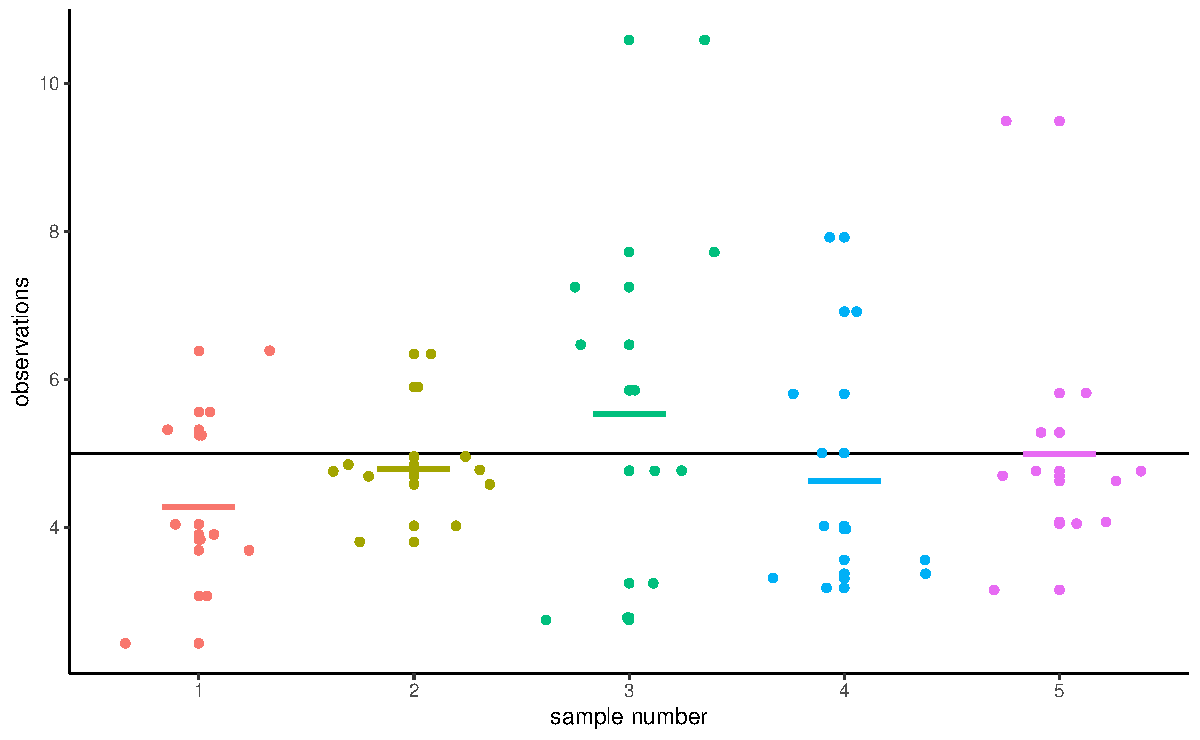
\includegraphics[width=0.85\textwidth,height=\textheight]{inference_files/figure-pdf/fig-samplevar-1.pdf}

}

\caption{\label{fig-samplevar}Five samples of size \(n=10\) drawn from a
common population with mean \(\mu\) (horizontal line). The colored
segments show the sample means of each sample.}

\end{figure}%

The astute eye might even notice that the sample means (thick horizontal
segments) are less dispersed around the full black horizontal line
representing the population average \(\mu\) than are the individual
measurements. This is a fundamental principle of statistics: information
accumulates as you get more data.

Values of the sample mean don't tell the whole picture and studying
differences in mean (between groups, or relative to a postulated
reference value) is not enough to draw conclusions. In most settings,
there is no guarantee that the sample mean will be equal to it's true
value because it changes from one sample to the next: the only guarantee
we have is that it will be on average equal to the population average in
repeated samples. Depending on the choice of measurement and variability
in the population, there may be considerable differences from one
observation to the next and this means the observed difference could be
a fluke.

To get an idea of how certain something is, we have to consider the
variability of an observation \(Y_i.\) This variance of an observation
drawn from the population is typically denoted \(\sigma^2\) and it's
square root, the standard deviation, by \(\sigma.\)

The standard deviation \emph{of a statistic} is termed \textbf{standard
error}; it should not be confused with the standard deviation \(\sigma\)
of the population from which the sample observations
\(Y_1, \ldots, Y_n\) are drawn. Both standard deviation and standard
error are expressed in the same units as the measurements, so are easier
to interpret than variance. Since the standard error is a function of
the sample size, it is however good practice to report the estimated
standard deviation in reports.

\begin{example}[Sample proportion and uniform
draws]\protect\hypertarget{exm-samppropunif}{}\label{exm-samppropunif}

To illustrate the concept of sampling variability, we follow the lead of
\href{https://www.crumplab.com/statistics/foundations-for-inference.html}{Matthew
Crump} and consider samples from a uniform distribution on
\(\{1, 2, \ldots, 10\}\) each number in this interval is equally likely
to be sampled.

\begin{figure}[ht!]

\centering{

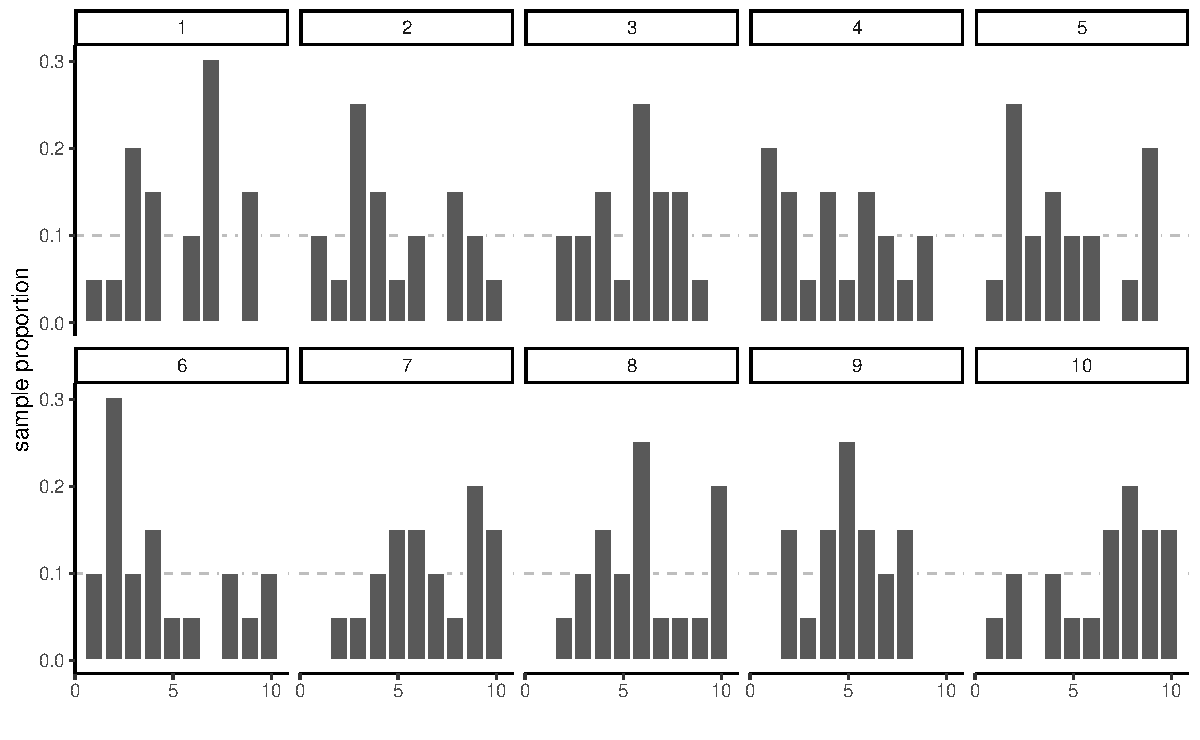
\includegraphics[width=0.85\textwidth,height=\textheight]{inference_files/figure-pdf/fig-unifsamp1-1.pdf}

}

\caption{\label{fig-unifsamp1}Histograms for 10 random samples of size
\(n=20\) from a discrete uniform distribution.}

\end{figure}%

Even if they are drawn from the same population, the 10 samples in
Figure~\ref{fig-unifsamp1} look quite different. The only thing at play
here is the sample variability: since there are \(n=20\) observations in
total, there should be on average 10\% of the observations in each of
the 10 bins, but some bins are empty and others have more counts than
expected. This fluctuation is due to randomness, or chance.

How can we thus detect whether what we see is compatible with the model
we think generated the data? The key is to collect more observations:
the bar height is the sample proportion, an average of 0/1 values with
ones indicating that the observation is in the bin and zero otherwise.

Consider now what happens as we increase the sample size: the top panel
of Figure~\ref{fig-uniformsamp2} shows uniform samples for increasing
samples size. The scaled bar plot looks more and more like the true
underlying distribution (flat, each bin with equal frequency) as the
sample size increases. The sample distribution of points is nearly
indistinguishable from the theoretical one (straight line) when
\(n=10 000.\)\footnote{The formula shows that the standard error
  decreases by a tenfold every time the sample size increases by a
  factor 100.} The bottom panel, on the other hand, isn't from a uniform
distribution and larger samples come closer to the population
distribution. We couldn't have spotted this difference in the first two
plots, since the sampling variability is too important; there, the lack
of data in some bins could have been attributed to chance, as they are
comparable with the graph for data that are truly uniform. This is in
line with most practical applications, in which the limited sample size
restricts our capacity to disentangle real differences from sampling
variability. We must embrace this uncertainty: in the next section, we
outline how hypothesis testing helps us disentangle the signal from the
noise.

\begin{figure}[ht!]

\centering{

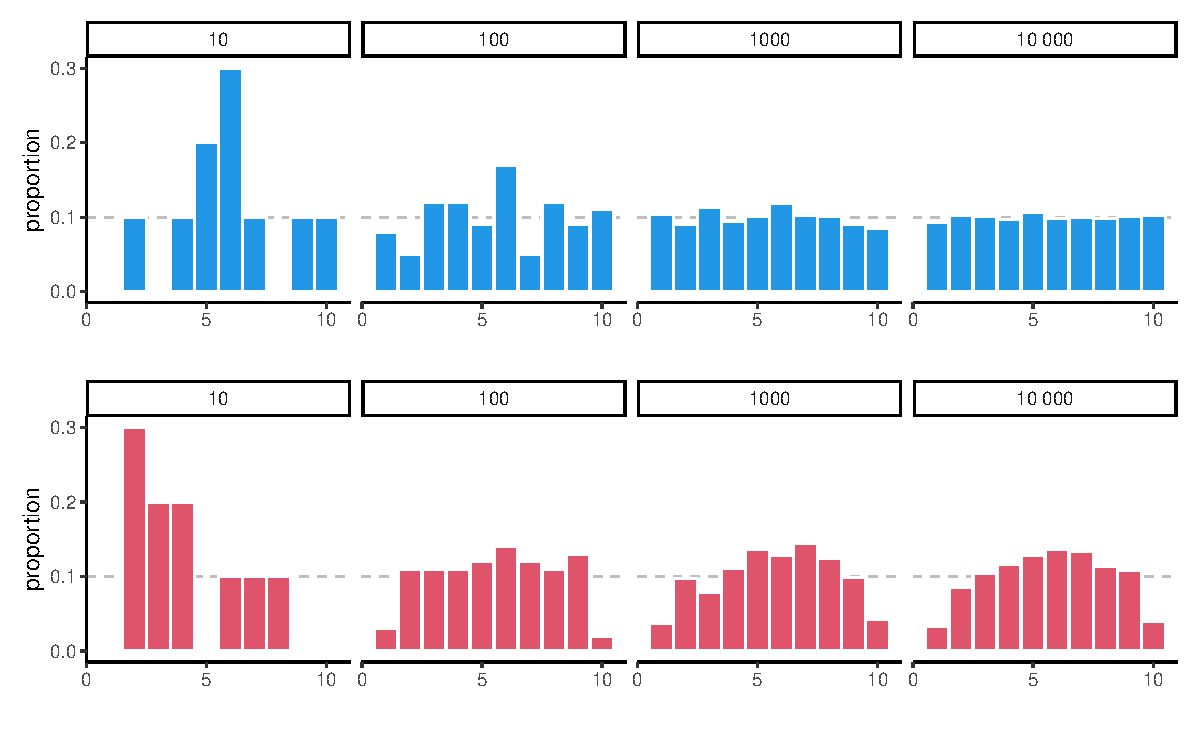
\includegraphics[width=0.85\textwidth,height=\textheight]{inference_files/figure-pdf/fig-uniformsamp2-1.pdf}

}

\caption{\label{fig-uniformsamp2}Bar plots of data from a uniform
distribution (top) and non-uniform (bottom) with increasing sample sizes
of 10, 100, 1000 and 10 000 (from left to right).}

\end{figure}%

\end{example}

\section{Hypothesis testing}\label{tests}

An \textbf{hypothesis test} is a binary decision rule used to evaluate
the statistical evidence provided by a sample to make a decision
regarding the underlying population. The main steps involved are:

\begin{itemize}
\tightlist
\item
  define the model parameters
\item
  formulate the alternative and null hypothesis
\item
  choose and calculate the test statistic
\item
  obtain the null distribution describing the behaviour of the test
  statistic under \(\mathscr{H}_0\)
\item
  calculate the \emph{p}-value
\item
  conclude (reject or fail to reject \(\mathscr{H}_0\)) in the context
  of the problem.
\end{itemize}

A good analogy for hypothesis tests is a trial for murder on which you
are appointed juror.

\begin{itemize}
\tightlist
\item
  The judge lets you choose between two mutually exclusive outcome,
  guilty or not guilty, based on the evidence presented in court.
\item
  The presumption of innocence applies and evidences are judged under
  this optic: are evidence remotely plausible if the person was
  innocent? The burden of the proof lies with the prosecution to avoid
  as much as possible judicial errors. The null hypothesis
  \(\mathscr{H}_0\) is \emph{not guilty}, whereas the alternative
  \(\mathscr{H}_a\) is \emph{guilty}. If there is a reasonable doubt,
  the verdict of the trial will be not guilty.
\item
  The test statistic (and the choice of test) represents the summary of
  the proof. The more overwhelming the evidence, the higher the chance
  the accused will be declared guilty. The prosecutor chooses the proof
  so as to best outline this: the choice of evidence (statistic)
  ultimately will maximise the evidence, which parallels the power of
  the test.
\item
  The final step is the verdict. This is a binary decision, guilty or
  not guilty. For an hypothesis test performed at level \(\alpha,\) one
  would reject (guilty) if the \emph{p}-value is less than \(\alpha.\)
\end{itemize}

The above description provides some heuristic, but lacks crucial
details.

\section{Hypothesis}\label{hypothesis}

In statistical tests we have two hypotheses: the null hypothesis
(\(\mathscr{H}_0\)) and the alternative hypothesis (\(\mathscr{H}_1\)).
Usually, the null hypothesis is the `status quo' and the alternative is
what we're really interested in testing. A statistical hypothesis test
allows us to decide whether or not our data provides enough evidence to
reject \(\mathscr{H}_0\) in favour of \(\mathscr{H}_1,\) subject to some
pre-specified risk of error. Usually, hypothesis tests involve a
parameter, say \(\theta,\) which characterizes the underlying
distribution at the population level ans whose value is unknown. A
two-sided hypothesis test regarding a parameter \(\theta\) has the form
\begin{align*}
\mathscr{H}_0: \theta=\theta_0 \qquad \text{versus} \qquad \mathscr{H}_a:\theta \neq \theta_0.
\end{align*} We are testing whether or not \(\theta\) is precisely equal
to the value \(\theta_0.\) The hypotheses are a statistical
representation of our research question.

A common example of two-sided test is one for the regression coefficient
\(\beta_j\) associated to an explanatory variable \(\mathrm{X}_j,\) for
which the null and alternative hypothesis are \begin{align*}
\mathscr{H}_0: \beta_j=\beta_j^0 \qquad \text{versus} \qquad \mathscr{H}_a:\beta_j \neq \beta_j^0,
\end{align*} where \(\beta_j^0\) is some value that reflects the
research question of interest. For example, if \(\beta_j^0=0,\) the
underlying question is: is covariate \(\mathrm{X}_j\) impacting the
response \(Y\) linearly once other variables have been taken into
account?

Note that we can impose direction in the hypotheses and consider
alternatives of the form \(\mathscr{H}_a: \theta > \theta_0\) or
\(\mathscr{H}_a: \theta < \theta_0.\)

\section{Test statistic}\label{test-statistic}

A test statistic \(T\) is a function of the data that summarise the
information contained in the sample for \(\theta.\) The form of the test
statistic is chosen such that we know its underlying distribution under
\(\mathscr{H}_0,\) that is, the potential values taken by \(T\) and
their relative probability if \(\mathscr{H}_0\) is true. Indeed, \(Y\)
is a random variable and its value change from one sample to the next.
This allows us to determine what values of \(T\) are likely if
\(\mathscr{H}_0\) is true. Many statistics we will consider are
\textbf{Wald statistic}, of the form \begin{align*}
T = \frac{\widehat{\theta} - \theta_0}{\mathrm{se}(\widehat{\theta})}
\end{align*} where \(\widehat{\theta}\) is an estimator of \(\theta,\)
\(\theta_0\) is the postulated value of the parameter and
\(\mathrm{se}(\widehat{\theta})\) is an estimator of the standard
deviation of the test statistic \(\widehat{\theta}.\)

For example, to test whether the mean of a population is zero, we set
\begin{align*}
\mathscr{H}_0: \mu=0, \qquad  \mathscr{H}_a:\mu \neq 0,
\end{align*} and the Wald statistic is \begin{align*}
T &= \frac{\overline{X}-0}{S_n/\sqrt{n}}
\end{align*} where \(\overline{X}\) is the sample mean of
\(X_1, \ldots, X_n,\) \begin{align*}
\overline{X} &= \frac{1}{n} \sum_{i=1}^n X_i = \frac{X_1+ \cdots + X_n}{n}
\end{align*} and the standard error (of the mean) \(\overline{X}\) is
\(S_n/\sqrt{n}\); the sample variance \(S_n\) is an estimator of the
standard deviation \(\sigma,\) \begin{align*}
S^2_n &= \frac{1}{n-1} \sum_{i=1}^n (X_i-\overline{X})^2.
\end{align*}

\section{\texorpdfstring{Null distribution and
\emph{p}-value}{Null distribution and p-value}}\label{null-distribution-and-p-value}

The \emph{p}-value allows us to decide whether the observed value of the
test statistic \(T\) is plausible under \(\mathscr{H}_0.\) Specifically,
the \emph{p}-value is the probability that the test statistic is equal
or more extreme to the estimate computed from the data, assuming
\(\mathscr{H}_0\) is true. Suppose that based on a random sample
\(Y_1, \ldots, Y_n\) we obtain a statistic whose value \(T=t.\) For a
two-sided test \(\mathscr{H}_0:\theta=\theta_0\)
vs.~\(\mathscr{H}_a:\theta \neq \theta_0,\) the \emph{p}-value is
\(\Pr_0(|T| \geq |t|).\)\footnote{If the distribution of \(T\) is
  symmetric around zero, the \emph{p}-value reduces to
  \(p = 2 \times \Pr_0(T \geq |t|).\)}

How do we determine the null distribution given that the true data
generating mechanism is unknown to us? We ask a statistician! In simple
cases, it might be possible to enumerate all possible outcomes and thus
quantity the degree of outlyingness of our observed statistic. In more
general settings, we can resort to simulations or to probability theory:
the central limit theorem says that the sample mean behaves like a
normal random variable with mean \(\mu\) and standard deviation
\(\sigma/\sqrt{n}\) for \(n\) large enough. The central limit theorem
has broader applications since most statistics can be viewed as some
form of average or transformation thereof, a fact used to derive
benchmarks for most commonly used tests. Most software use these
approximations as proxy by default: the normal, Student's \(t,\)
\(\chi^2\) and \(F\) distributions are the reference distributions that
arise the most often.

Figure~\ref{fig-power-plots} shows the distribution of \(p\)-values for
two scenarios: one in which there are no differences and the null is
true, the other under an alternative. The probability of rejection is
obtained by calculating the area under the density curve between zero
and \(\alpha=0.1,\) here 0.1 on the left. Under the null, the model is
calibrated and the distribution of \emph{p}-values is uniform (i.e., a
flat rectangle of height 1), meaning all values in the unit interval are
equally likely. Under the alternative (right), small \emph{p}-values are
more likely to be observed.

\begin{figure}[ht!]

\centering{

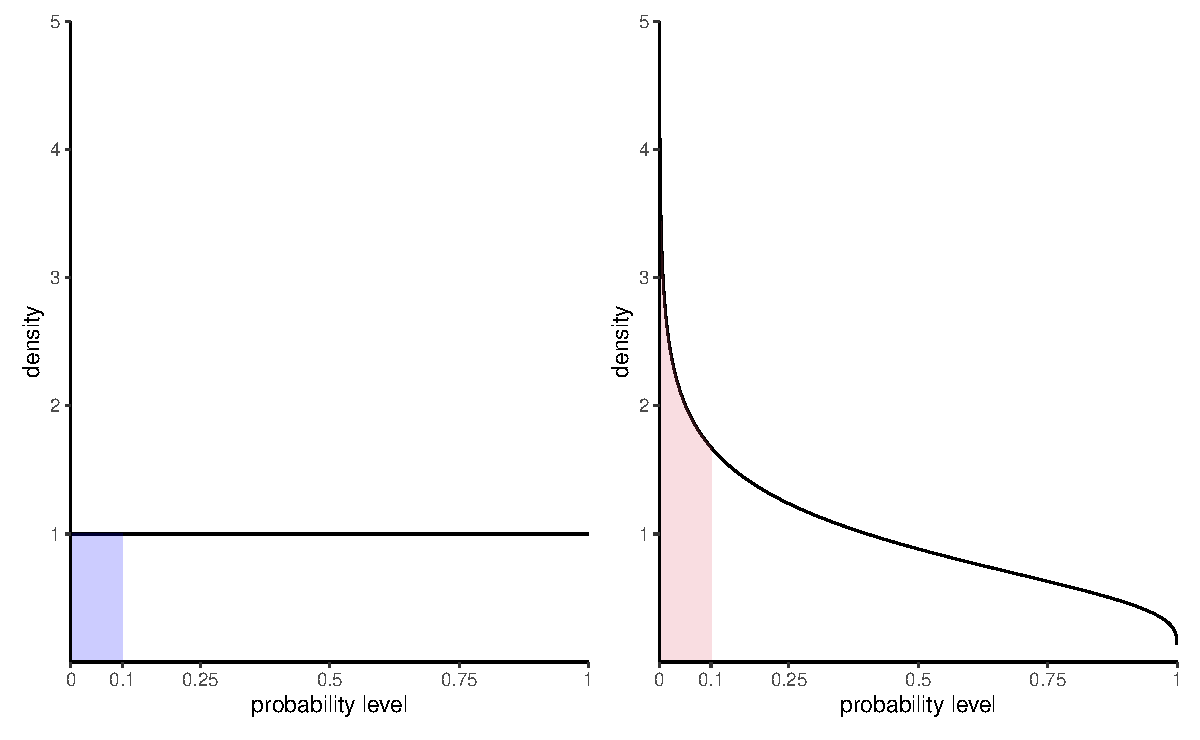
\includegraphics[width=0.85\textwidth,height=\textheight]{inference_files/figure-pdf/fig-power-plots-1.pdf}

}

\caption{\label{fig-power-plots}Density of \emph{p}-values under the
null hypothesis (left) and under an alternative with a signal-to-noise
ratio of 0.5 (right).}

\end{figure}%

There are generally three ways of obtaining null distributions for
assessing the degree of evidence against the null hypothesis

\begin{itemize}
\tightlist
\item
  exact calculations
\item
  large sample theory (aka `asymptotics' in statistical lingo)
\item
  simulation
\end{itemize}

While desirable, the first method is only applicable in simple cases
(such as counting the probability of getting two six if you throw two
fair die). The second method is most commonly used due to its generality
and ease of use (particularly in older times where computing power was
scarce), but fares poorly with small sample sizes (where `too small' is
context and test-dependent). The last approach can be used to
approximate the null distribution in many scenarios, but adds a layer of
randomness and the extra computations costs sometimes are not worth it.

Consider the example of a two-sided test involving the population mean
\(\mathscr{H}_0:\mu=0\) against the alternative
\(\mathscr{H}_1:\mu \neq 0.\) Assuming the random sample comes from a
normal (population) \(\mathsf{normal}(\mu, \sigma^2),\) it can be shown
that if \(\mathscr{H}_0\) is true (that is, if \(\mu=0\)), the test
statistic \begin{align*}
T = \frac{\overline{X}}{S/\sqrt{n}}
\end{align*} follows a Student-\emph{t} distribution with \(n-1\)
degrees of freedom. This allows us to calculate the \emph{p}-value
(either from a table, or using some statistical software). By virtue of
the symmetry, the \emph{p}-value is \(P = 2\times\Pr(T > |t|),\) where
\(T \sim \mathsf{Student}(n-1).\)

\section{Confidence intervals}\label{confidence-intervals}

A \textbf{confidence interval} is an alternative way to present the
conclusions of an hypothesis test performed at significance level
\(\alpha.\) It is often combined with a point estimator \(\hat{\theta}\)
plus or minus a margin of error designed to give an indication of the
variability of the estimation procedure. Wald-based \((1-\alpha)\)
confidence intervals for a scalar parameter \(\theta\) are of the form
\begin{align*}
[\widehat{\theta} + \mathfrak{q}_{\alpha/2}\mathrm{se}(\widehat{\theta}), \widehat{\theta} +\mathfrak{q}_{1-\alpha/2}\times \mathrm{se}(\widehat{\theta})]
\end{align*} where \(\mathfrak{q}_{\alpha/2}\) is the \(\alpha/2\)
quantile of the null distribution of the Wald statistic \(W,\)
\begin{align*}
W =\frac{\widehat{\theta}-\theta}{\mathrm{se}(\widehat{\theta})},
\end{align*} and where \(\theta\) represents the postulated value for
the fixed, but unknown value of the parameter. The critical values for a
symmetric interval, chosen so that the probability of being more extreme
is \(\alpha\), are the \(\alpha/2\) and \(1-\alpha/2\) quantiles of the
null distribution.

For example, for a random sample \(X_1, \ldots, X_n\) from a normal
distribution \(\mathsf{normal}(\mu, \sigma),\) the (\(1-\alpha\))
confidence interval for the population mean \(\mu\) is \begin{align*}
\overline{X} \pm t_{n-1, \alpha/2} \frac{S}{\sqrt{n}}
\end{align*} where \(t_{n-1,\alpha/2}\) is the \(1-\alpha/2\) quantile
of a Student-\(t\) distribution with \(n-1\) degrees of freedom.

The bounds of the confidence intervals are random variables, since both
estimators of the parameter and its standard error, \(\widehat{\theta}\)
and \(\mathrm{se}(\widehat{\theta}),\) are random: their values will
vary from one sample to the next. Before the interval is calculated,
there is a \(1-\alpha\) probability that \(\theta\) is contained in the
\textbf{random} interval
\((\widehat{\theta} - \mathfrak{q}_{\alpha/2} \; \mathrm{se}(\widehat{\theta}), \widehat{\theta} + \mathfrak{q}_{\alpha/2} \; \mathrm{se}(\widehat{\theta})),\)
where \(\widehat{\theta}\) denotes the estimator. Once we obtain a
sample and calculate the confidence interval, there is no more notion of
probability: the true value of the parameter \(\theta\) is either in the
confidence interval or not. We can interpret confidence intervals as
follows: if we were to repeat the experiment multiple times, and
calculate a \(1-\alpha\) confidence interval each time, then roughly
\(1-\alpha\) of the calculated confidence intervals would contain the
true value of \(\theta\) in repeated samples (in the same way, if you
flip a coin, there is roughly a 50-50 chance of getting heads or tails,
but any outcome will be either). Our confidence is in the
\emph{procedure} we use to calculate confidence intervals and not in the
actual values we obtain from a sample.

\begin{figure}[ht!]

{\centering 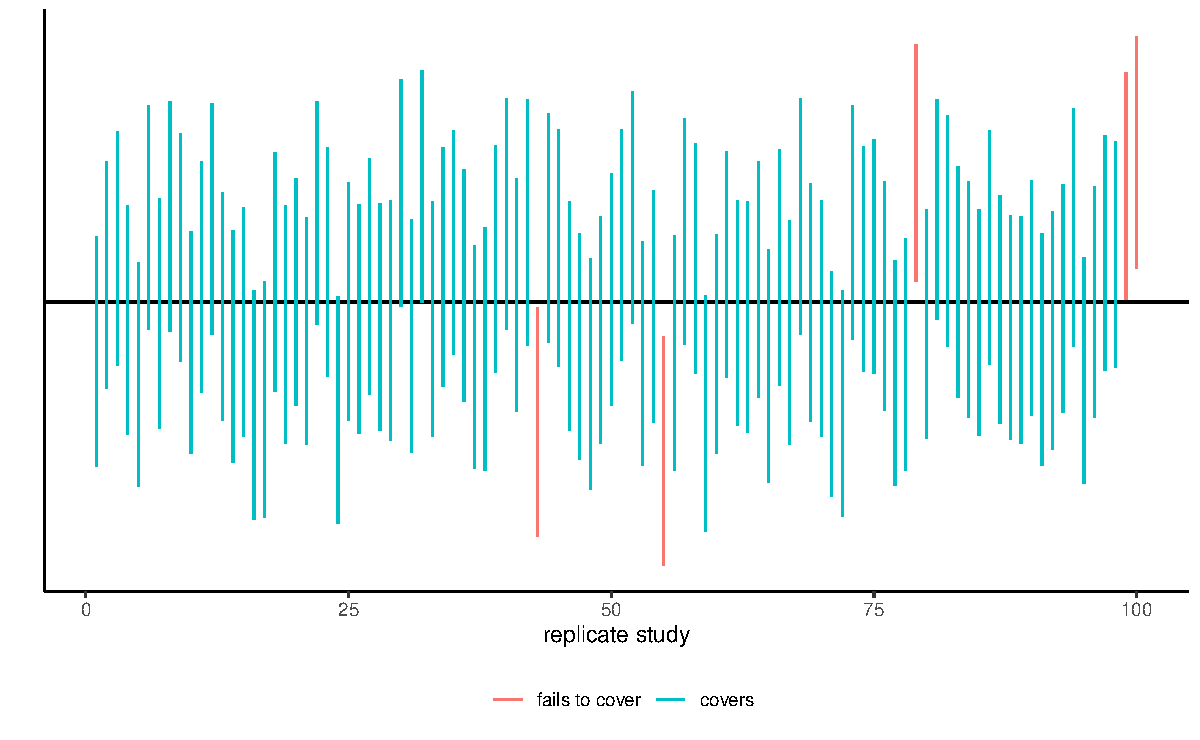
\includegraphics[width=0.85\textwidth,height=\textheight]{inference_files/figure-pdf/intconf-1.pdf}

}

\caption{95\% confidence intervals for the mean of a standard normal
population for 100 random samples. On average, 5\% of these intervals
fail to include the true mean value of zero (in red).}

\end{figure}%

If we are only interested in the binary decision rule reject/fail to
reject \(\mathscr{H}_0,\) the confidence interval is equivalent to a
\emph{p}-value since it leads to the same conclusion. Whereas the
\(1-\alpha\) confidence interval gives the set of all values for which
the test statistic doesn't provide enough evidence to reject
\(\mathscr{H}_0\) at level \(\alpha,\) the \emph{p}-value gives the
probability under the null of obtaning a result more extreme than the
postulated value and so is more precise for this particular value. If
the \emph{p}-value is smaller than \(\alpha,\) our null value \(\theta\)
will be outside of the confidence interval and vice-versa.

\section{Conclusion}\label{conclusion}

The \emph{p}-value allows us to make a decision about the null
hypothesis. If \(\mathscr{H}_0\) is true, the \emph{p}-value follows a
uniform distribution. \href{https://xkcd.com/1478/}{Thus, if the
\emph{p}-value is small}, this means observing an outcome more extreme
than \(T=t\) is unlikely, and so we're inclined to think that
\(\mathscr{H}_0\) is not true. There's always some underlying risk that
we're making a mistake when we make a decision. In statistic, there are
\href{https://xkcd.com/2303/}{two type of errors}:

\begin{itemize}
\tightlist
\item
  type I error: we reject \(\mathscr{H}_0\) when \(\mathscr{H}_0\) is
  true,
\item
  type II error: we fail to reject \(\mathscr{H}_0\) when
  \(\mathscr{H}_0\) is false.
\end{itemize}

These hypothesis are not judged equally: we seek to avoid error of type
I (judicial errors, corresponding to condemning an innocent). To prevent
this, we fix the level of the test, \(\alpha,\) which captures our
tolerance to the risk of committing a type I error: the higher the level
of the test \(\alpha,\) the more often we will reject the null
hypothesis when the latter is true. The value of \(\alpha \in (0, 1)\)
is the probability of rejecting \(\mathscr{H}_0\) when \(\mathscr{H}_0\)
is in fact true, \begin{align*}
\alpha = \Pr{}_0\left(\text{ reject } \mathscr{H}_0\right).
\end{align*} where the subscript \(\Pr{}_0\) indicates the probability
under the null model. The level \(\alpha\) is fixed beforehand,
typically \(1\)\%, \(5\)\% or \(10\)\%. Keep in mind that the
probability of type I error is \(\alpha\) only if the null model for
\(\mathscr{H}_0\) is correct (sic) and correspond to the data generating
mechanism.

The focus on type I error is best understood by thinking about medical
trial: you need to prove a new cure is better than existing alternatives
drugs or placebo, to avoid extra costs or harming patients (think of
Didier Raoult and his unsubstantiated claims that hydrochloroquine, an
antipaludean drug, should be recommended treatment against Covid19).

\begin{longtable}[]{@{}lcc@{}}
\toprule\noalign{}
\textbf{Decision} \textbackslash{} \textbf{true model} &
\(\mathscr{H}_0\) & \(\mathscr{H}_a\) \\
\midrule\noalign{}
\endhead
\bottomrule\noalign{}
\endlastfoot
fail to reject \(\mathscr{H}_0\) & \(\checkmark\) & type II error \\
reject \(\mathscr{H}_0\) & type I error & \(\checkmark\) \\
\end{longtable}

To make a decision, we compare our \emph{p}-value \(P\) with the level
of the test \(\alpha\):

\begin{itemize}
\tightlist
\item
  if \(P < \alpha,\) we reject \(\mathscr{H}_0\);
\item
  if \(P \geq \alpha,\) we fail to reject \(\mathscr{H}_0.\)
\end{itemize}

Do not mix up level of the test (probability fixed beforehand by the
researcher) and the \emph{p}-value. If you do a test at level 5\%, the
probability of type I error is by definition \(\alpha\) and does not
depend on the \emph{p}-value. The latter is conditional probability of
observing a more extreme likelihood given the null distribution
\(\mathscr{H}_0\) is true.

\begin{tcolorbox}[enhanced jigsaw, coltitle=black, colframe=quarto-callout-caution-color-frame, breakable, opacityback=0, title=\textcolor{quarto-callout-caution-color}{\faFire}\hspace{0.5em}{Caution}, left=2mm, arc=.35mm, colbacktitle=quarto-callout-caution-color!10!white, opacitybacktitle=0.6, titlerule=0mm, rightrule=.15mm, bottomtitle=1mm, toptitle=1mm, leftrule=.75mm, colback=white, toprule=.15mm, bottomrule=.15mm]

The \href{https://doi.org/10.1080/00031305.2016.1154108}{American
Statistical Association (ASA) published a list of principles} guiding
(mis)interpretation of \emph{p}-values, some of which are reproduced
below:

\begin{quote}
\begin{enumerate}
\def\labelenumi{(\arabic{enumi})}
\setcounter{enumi}{1}
\tightlist
\item
  \emph{P}-values do not measure the probability that the studied
  hypothesis is true.
\end{enumerate}
\end{quote}

\begin{quote}
\begin{enumerate}
\def\labelenumi{(\arabic{enumi})}
\setcounter{enumi}{2}
\tightlist
\item
  Scientific conclusions and business or policy decisions should not be
  based only on whether a \emph{p}-value passes a specific threshold.
\end{enumerate}
\end{quote}

\begin{quote}
\begin{enumerate}
\def\labelenumi{(\arabic{enumi})}
\setcounter{enumi}{3}
\tightlist
\item
  \emph{P}-values and related analyses should not be reported
  selectively.
\end{enumerate}
\end{quote}

\begin{quote}
\begin{enumerate}
\def\labelenumi{(\arabic{enumi})}
\setcounter{enumi}{4}
\tightlist
\item
  \emph{p}-value, or statistical significance, does not measure the size
  of an effect or the importance of a result.
\end{enumerate}
\end{quote}

\end{tcolorbox}

\section{Power}\label{power}

There are two sides to an hypothesis test: either we want to show it is
not unreasonable to assume the null hypothesis, or else we want to show
beyond reasonable doubt that a difference or effect is significative:
for example, one could wish to demonstrate that a new website design
(alternative hypothesis) leads to a significant increase in sales
relative to the status quo. Our ability to detect these improvements and
make discoveries depends on the power of the test: the larger the power,
the greater our ability to reject \(\mathscr{H}_0\) when the latter is
false.

Failing to reject \(\mathscr{H}_0\) when \(\mathscr{H}_a\) is true
corresponds to the definition of type II error, the probability of which
is \(1-\text{power},\) say. The \textbf{power of a test} is the
probability of rejecting \(\mathscr{H}_0\) when \(\mathscr{H}_0\) is
false, i.e., \begin{align*}
\Pr{\!}_a(\text{reject } \mathscr{H}_0),
\end{align*} i.e., the probability under the alternative model of
falling in the rejection region. Depending on the alternative models, it
is more or less easy to detect that the null hypothesis is false and
reject in favor of an alternative.

\begin{figure}[ht!]

\centering{

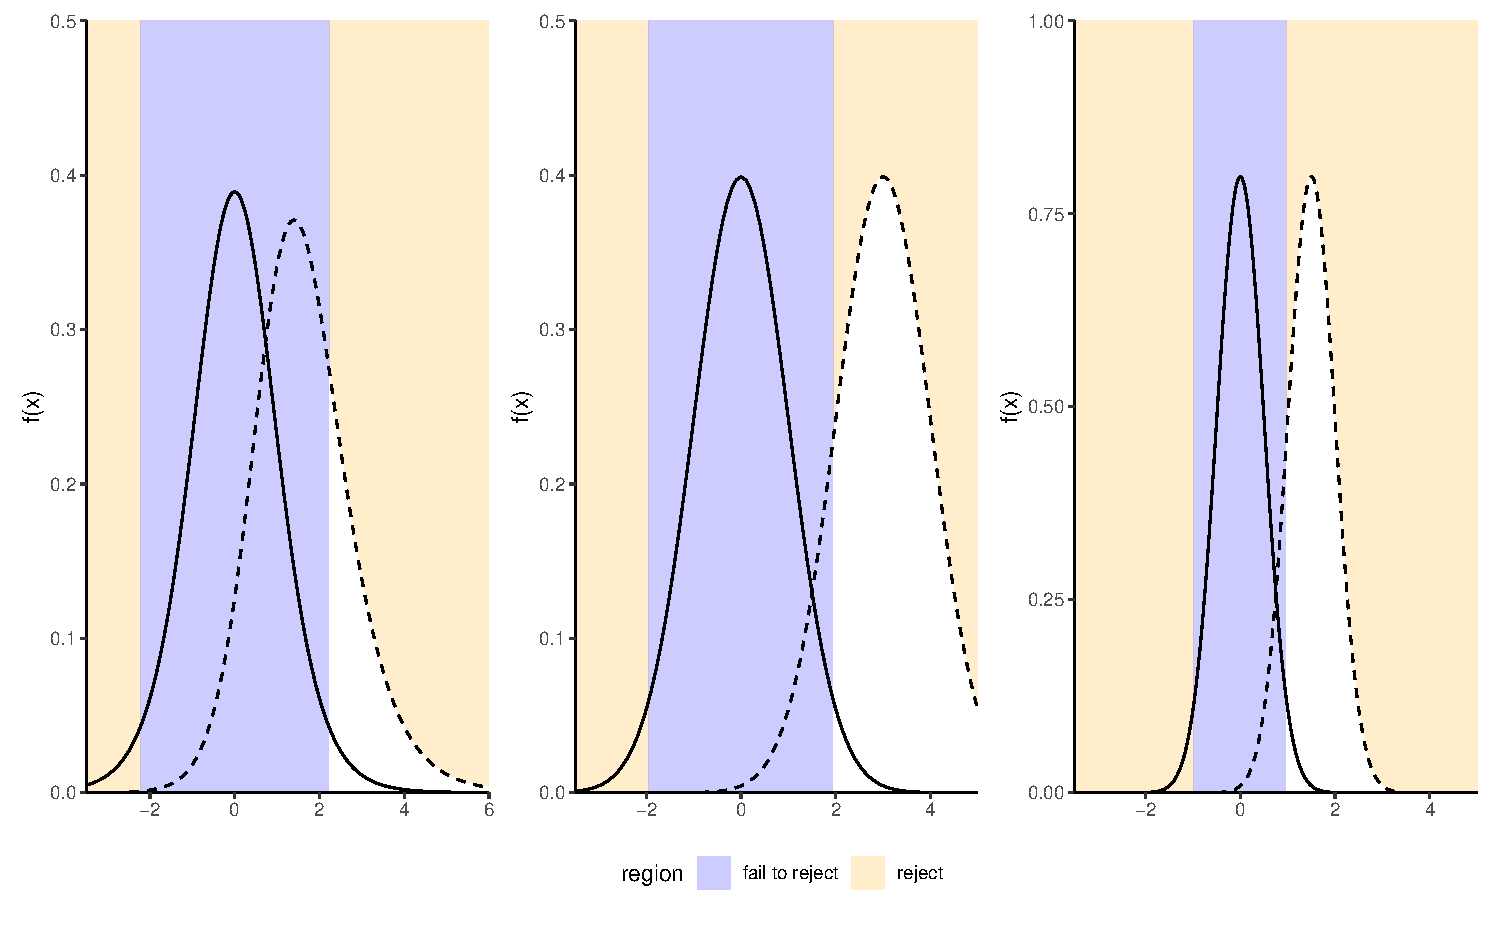
\includegraphics[width=1\textwidth,height=\textheight]{inference_files/figure-pdf/fig-power-1.pdf}

}

\caption{\label{fig-power}Comparison between null distribution (full
curve) and a specific alternative for a \emph{t}-test (dashed line). The
power corresponds to the area under the curve of the density of the
alternative distribution which is in the rejection area (in white). The
middle panel shows an increase in power due to an increase in the mean
difference, whereas the right panel shows the change due to a decrease
in variability of increase in the sample size.}

\end{figure}%

We want a test to have high power, i.e., that the power should be as
close to 1 as possible. Minimally, the power of the test should be
\(\alpha\) because we reject the null hypothesis \(\alpha\) fraction of
the time even when \(\mathscr{H}_0\) is true. Power depends on many
criteria, notably

\begin{itemize}
\tightlist
\item
  the effect size: the bigger the difference between the postulated
  value for \(\theta_0\) under \(\mathscr{H}_0\) and the observed
  behavior, the easier it is to detect it, as in the middle panel of
  Figure~\ref{fig-power};
\item
  variability: the less noisy your data, the easier it is to detect
  differences between the curves (big differences are easier to spot, as
  the right panel of Figure~\ref{fig-power} shows);
\item
  the sample size: the more observation, the higher our ability to
  detect significative differences because the standard error decreases
  with sample size \(n\) at a rate (typically) of \(n^{-1/2}.\) The null
  distribution also becomes more concentrated as the sample size
  increase.
\item
  the choice of test statistic: for example, rank-based statistics
  discard information about the actual values and care only about
  relative ranking. Resulting tests are less powerful, but are typically
  more robust to model misspecification and outliers. The statistics we
  will choose are standard and amongst the most powerful: as such, we
  won't dwell on this factor.
\end{itemize}

To calculate the power of a test, we need to single out a specific
alternative hypothesis. In very special case, analytic derivations are
possible but typically we compute the power of a test through Monte
Carlo methods. For a given alternative, we simulate repeatedly samples
from the model, compute the test statistic on these new samples and the
associated \emph{p}-values based on the postulated null hypothesis. We
can then calculate the proportion of tests that lead to a rejection of
the null hypothesis at level \(\alpha,\) namely the percentage of
\emph{p}-values smaller than \(\alpha.\)

\section{Examples}\label{examples}

\begin{example}[Gender inequality and permutation
tests]\protect\hypertarget{exm-rosenjerdee74}{}\label{exm-rosenjerdee74}

We consider data from Rosen and Jerdee
(\citeproc{ref-Rosen:1974}{1974}), who look at sex role stereotypes and
their impacts on promotion and opportunities for women candidates. The
experiment took place in 1972 and the experimental units, which
consisted of 95 male bank supervisors, were submitted to various
memorandums and asked to provide ratings or decisions based on the
information provided.

We are interested in Experiment 1 related to promotion of employees:
managers were requested to decide on whether or not to promote an
employee to become branch manager based on recommendations and ratings
on potential for customer and employee relations.

The authors intervention focused on the description of the nature
(complexity) of the manager's job (either simple or complex) and the sex
of the candidate (male or female): all files were otherwise similar.

We consider for simplicity only sex as a factor and aggregate over job
for the \(n=93\) replies. Table~\ref{tbl-rosen-table1} shows the counts
for each possibility.

\begin{longtable}[t]{lrr}

\caption{\label{tbl-rosen-table1}Promotion recommandation to branch
manager based on sex of the applicant.}

\tabularnewline

\toprule
 & male & female\\
\midrule
promote & 32 & 19\\
hold file & 12 & 30\\
\bottomrule

\end{longtable}

The null hypothesis of interest here that sex has no impact, so the
probability of promotion is the same for men and women. Let
\(p_{\text{m}}\) and \(p_{\text{w}}\) denote these respective
probabilities; we can thus write mathematically the null hypothesis as
\(\mathscr{H}_0: p_{\text{m}} = p_{\text{w}}\) against the alternative
\(\mathscr{H}_a: p_{\text{m}} \neq p_{\text{w}}.\)

The test statistic typically employed for contingency tables is a
chi-square test\footnote{If you have taken advanced modelling courses,
  this is a score test obtained by fitting a Poisson regression with
  \texttt{sex} and \texttt{action} as covariates; the null hypothesis
  corresponding to lack of interaction term between the two.}, which
compares the overall proportions of promoted to that in for each
subgroup. The sample proportion for male is 32/42 = \textasciitilde76\%,
compared to 19/49 or \textasciitilde49\% for female. While it seems that
this difference of 16\% is large, it could be spurious: the standard
error for the sample proportions is roughly 3.2\% for male and 3.4\% for
female.

If there was no discrimination based on sex, we would expect the
proportion of people promoted to be the same overall; this is 51/93
=0.55 for the pooled sample. We could simply do a test for the mean
difference, but rely instead on the Pearson contingency \(X^2_p\) (aka
chi-square) test, which compares the expected counts (based on equal
promotion rates) to the observed counts, suitably standardized. If the
discrepancy is large between expected and observed, than this casts
doubt on the validity of the null hypothesis.

If the counts of each cell are large, the null distribution of the
chi-square test is well approximated by a \(\chi^2\) distribution. The
output of the test includes the value of the statistic, \(10.79,\) the
degrees of freedom of the \(\chi^2\) approximation and the
\emph{p}-value, which gives the probability that a random draw from a
\(\chi^2_1\) distribution is larger than the observed test statistic
\textbf{assuming the null hypothesis is true}. The \emph{p}-value is
very small, \(0.001,\) which means such a result is quite unlikely to
happen by chance if there was no sex-discrimination.

Another alternative to obtain a benchmark to assess the outlyingness of
the observed odds ratio is to use simulations: permutation tests are
well \href{https://www.jwilber.me/permutationtest/}{illustrated by Jared
Wilber}. Consider a database containing the raw data with 93 rows, one
for each manager, with for each an indicator of \texttt{action} and the
\texttt{sex} of the hypothetical employee presented in the task.

\begin{longtable}[t]{ll}

\caption{\label{tbl-dat-long-test-rosen-print}First five rows of the
database in long format for experiment 1 of Rosen and Jerdee.}

\tabularnewline

\toprule
action & sex\\
\midrule
promote & male\\
hold file & female\\
promote & male\\
hold file & female\\
hold file & male\\
\bottomrule

\end{longtable}

Under the null hypothesis, sex has no incidence on the action of the
manager. This means we could get an idea of the ``what-if'' world by
shuffling the sex labels repeatedly. Thus, we could obtain a benchmark
by repeating the following steps multiple times:

\begin{enumerate}
\def\labelenumi{\arabic{enumi}.}
\tightlist
\item
  permute the labels for \texttt{sex},
\item
  recreate a contingency table by aggregating counts,
\item
  calculate a test statistic for the simulated table.
\end{enumerate}

As test statistic, we use odds ratio: the odds of an event is the ratio
of the number of success over failure: in our example, this would be the
number of promoted over held files. The odds of promotion for male is
\(32/12,\) whereas that of female is \(19/30.\) The odds ratio for male
versus female is thus \(\mathsf{OR}=(32/12) / (19/30)= 4.21.\) Under the
null hypothesis, \(\mathscr{H}_0: \mathsf{OR}= 1\) (same probability of
being promoted) (why?)

\begin{figure}[ht!]

\centering{

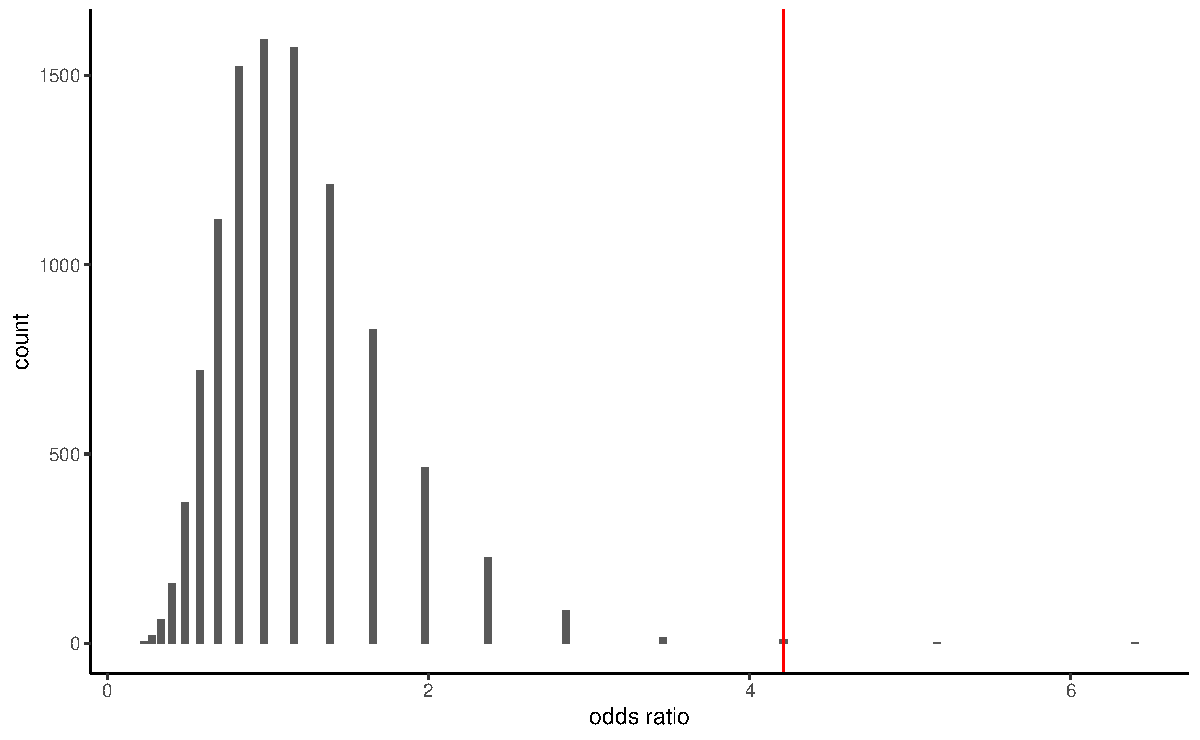
\includegraphics[width=0.85\textwidth,height=\textheight]{inference_files/figure-pdf/fig-infer-odds-ratio-permutation-1.pdf}

}

\caption{\label{fig-infer-odds-ratio-permutation}Histogram of the
simulated null distribution of the odds ratio statistic obtained using a
permutation test; the vertical red line indicates the sample odds
ratio.}

\end{figure}%

The histogram in Figure~\ref{fig-infer-odds-ratio-permutation} shows the
distribution of the odds ratio based on 10 000 permutations.
Reassuringly, we again get roughly the same approximate \emph{p}-value,
here 0.002.\footnote{The \emph{p}-value obtained for the permutation
  test would change from one run to the next since it's input is random.
  However, the precision of the proportion statistic is sufficient for
  decision making purposes.}

The article concluded (in light of the above and further experiments)

\begin{quote}
Results confirmed the hypothesis that male administrators tend to
discriminate against female employees in personnel decisions involving
promotion, development, and supervision.
\end{quote}

\textbf{Recap}

\begin{itemize}
\tightlist
\item
  Model parameters: probability of promotion for men and women,
  respectively \(p_{\text{m}}\) and \(p_{\text{w}}.\)
\item
  Hypotheses: no discrimination based on gender, meaning equal
  probability of promotion (null hypothesis
  \(\mathscr{H}_0: p_{\text{m}}=p_{\text{w}},\) versus alternative
  hypothesis \(\mathscr{H}_a: p_{\text{m}}\neq p_{\text{w}}\)).
\item
  Test statistic: (1) chi-square test for contingency tables and (2)
  odds ratio.
\item
  \(p\)-value: (1) \(.0010\) and (2) \(.0024\) based on permutation
  test.
\item
  Conclusion: reject null hypothesis, as there is evidence of a
  gender-discrimination with different probability of promotion for men
  and women.
\end{itemize}

Following the APA guidelines, the \(\chi^2\) statistic would be reported
as \(\chi^2(1, n = 93) = 10.79\), \(p = .001\) along with counts and
sample proportions.

\end{example}

\begin{example}[``The Surprise of Reaching
Out'']\protect\hypertarget{exm-LiuRimMinMin2023E1}{}\label{exm-LiuRimMinMin2023E1}

Liu et al. (\citeproc{ref-Liu.Rim.Min.Min:2023}{2023}) studies social
interactions and the impact of surprise on people reaching out if this
contact is unexpected. Experiment 1 focuses on questionnaires where the
experimental condition is the perceived appreciation of reaching out to
someone (vs being reached to). The study used a questionnaire
administered to 200 American adults recruited on the Prolific Academic
platform. The response index consists of the average of four questions
measured on a Likert scale ranging from 1 to 7, with higher values
indicating higher appreciation.

We can begin by inspecting summary statistics for the sociodemographic
variables (gender and age) to assess whether the sample is
representative of the general population as a whole. The proportion of
\texttt{other} (including non-binary people) is much higher than that of
the general census, and the population skews quite young according to
Table~\ref{tbl-LRMMS1-summarystat-a}.

\begin{longtable}[t]{lrrrr}

\caption{\label{tbl-LRMMS1-summarystat-a}Summary statistics of the age
of participants, and counts per gender}

\tabularnewline

\toprule
gender & min & max & mean & n\\
\midrule
male & 18 & 78 & 32.0 & 105\\
female & 19 & 68 & 36.5 & 92\\
other & 24 & 30 & 27.7 & 3\\
\bottomrule

\end{longtable}

\begin{longtable}[t]{lrrr}

\caption{\label{tbl-LRMMS1-summarystat-b}Mean ratings, standard
deviation and number of participants per experimental condition.}

\tabularnewline

\toprule
role & mean & sd & n\\
\midrule
initiator & 5.50 & 1.28 & 103\\
responder & 5.87 & 1.27 & 97\\
\bottomrule

\end{longtable}

Since there are only two groups, initiator and responder, we are dealing
with a pairwise comparison. The logical test one could use is a two
sample \emph{t}-test, or a variant thereof. Using Welch two sample
\(t\)-test statistic, both group average and standard deviation are
estimated using the data provided.

The software returns \(t(197.52) = -2.05\), \(p = .041\), which leads to
the rejection of the null hypothesis of no difference in appreciation
depending on the role of the individual (initiator or responder). The
estimated mean difference is \(\Delta M = -0.37\), 95\% CI
\([-0.73, -0.01]\); since \(0\) is not included in the confidence
interval, we also reject the null hypothesis at level 5\%. The estimate
suggests that initiators underestimate the appreciation of reaching
out.\footnote{Assuming that the variance of each subgroup were equal, we
  could have used a two-sample \(t\)-test instead. The difference in the
  conclusion is immaterial, with a nearly equal \emph{p}-value.}

\textbf{Recap}

\begin{itemize}
\tightlist
\item
  Model parameters: average expected appreciation score
  \(\mu_{\mathrm{i}}\) and \(\mu_{\mathrm{r}}\) of initiators and
  responder, respectively
\item
  Hypothesis: expected appreciation score is the same for initiator and
  responders, \(\mathscr{H}_0: \mu_{\mathrm{i}}=\mu_{\mathrm{r}}\)
  against alternative
  \(\mathscr{H}_a: \mu_{\mathrm{i}} \neq \mu_{\mathrm{r}}\) that they
  are different.
\item
  Test statistic: Welch two sample \(t\)-test
\item
  \(p\)-value: 0.041
\item
  Conclusion: reject the null hypothesis, average appreciation score
  differs depending on the role
\end{itemize}

\end{example}

\begin{example}[Virtual communication curbs creative idea
generation]\protect\hypertarget{exm-BrucksLevav22}{}\label{exm-BrucksLevav22}

A Nature study performed an experiment to see how virtual communications
teamwork by comparing the output both in terms of ideas generated during
a brainstorming session by pairs and of the quality of ideas, as
measured by external referees. The sample consisted of 301 pairs of
participants who interacted via either videoconference or face-to-face.

The authors compared the number of creative ideas, a subset of the ideas
generated with creativity score above average. The mean number of the
number of creative ideas for face-to-face \(7.92\) ideas (sd \(3.40\))
relative to videoconferencing \(6.73\) ideas (sd \(3.27\)).

Brucks and Levav (\citeproc{ref-Brucks.Levav:2022}{2022}) used a
negative binomial regression model: in their model, the expected number
creative ideas generated is \begin{align*}
\mathsf{E}(\texttt{ncreative}) = \exp(\beta_0 + \beta_1 \texttt{video})
\end{align*} where \(\texttt{video}=0\) if the pair are in the same room
and \(\texttt{video}=1\) if they interact instead via videoconferencing.

The mean number of ideas for videoconferencing is thus \(\exp(\beta_1)\)
times that of the face-to-face: the estimate of the multiplicative
factor is \(\exp(\beta_1)\) is \(0.85\) 95\% CI \([0.77, 0.94]\).

No difference between experimental conditions translates into the null
hypothesis as \(\mathscr{H}_0: \beta_1=0\) vs
\(\mathscr{H}_0: \beta_1 \neq 0\) or equivalently
\(\mathscr{H}_0: \exp(\beta_1)=1.\) The likelihood ratio test comparing
the regression model with and without \(\texttt{video}\) the statistic
is \(R=9.89\) (\(p\)-value based on \(\chi^2_1\) of \(.002\)). We
conclude the average number of ideas is different, with summary
statistics suggesting that virtual pairs generate fewer ideas.

If we had resorted to a two sample \(t\)-test, we would have found a
mean difference in the number of creative idea of \(\Delta M = 1.19\),
95\% CI \([0.43, 1.95]\), \(t(299) = 3.09\), \(p = .002\).

Both tests come with slightly different sets of assumptions, but yield
similar conclusions: there is evidence of a smaller number of creative
ideas when people interact via videoconferencing.

\end{example}

\begin{example}[Price of Spanish high speed train
tickets]\protect\hypertarget{exm-price-trains-tests}{}\label{exm-price-trains-tests}

The Spanish national railway company,
\href{https://www.renfe.com/}{Renfe}, manages regional and high speed
train tickets all over Spain and The Gurus
\href{https://www.kaggle.com/thegurusteam/spanish-high-speed-rail-system-ticket-pricing}{harvested}
the price of tickets sold by Renfe. We are interested in trips between
Madrid and Barcelona and, for now, ask the question: are tickets more
expensive one way or another? To answer this, we consider a sample of
8059 AVE tickets sold at Promo rate. Our test statistic will again be
the mean difference between the price (in euros) for a train ticket for
Madrid--Barcelona (\(\mu_1\)) and the price for Barcelona--Madrid
(\(\mu_2\)), i.e., \(\mu_1-\mu_2.\) The null hypothesis is that there
are no difference in price, so \(\mathscr{H}_0: \mu_1-\mu_2=0.\)

We use Welch's \(t\) test statistic for two samples: the sample mean of
the price of Barcelona-Madrid tickets is 82.15 euros, that of
Madrid-Barcelona tickets is 82.54 euros and the Welch statistic is worth
-1.15. If we use a normal approximation, the \emph{p}-value is 0.25.

Rather than use the asymptotic distribution, whose validity stems from
the central limit theorem, we could consider another approximation under
the less restrictive assumption that the data are exchangeable: under
the null hypothesis, there is no difference between the two destinations
and so the label for destination (a binary indicator) is arbitrary. The
reasoning underlying
\href{https://www.jwilber.me/permutationtest/}{permutation tests} is as
follows: to create a benchmark, we will consider observations with the
same number in each group, but permuting the labels. We then compute the
test statistic on each of these datasets. If there are only a handful in
each group (fewer than 10), we could list all possible permutations of
the data, but otherwise we can repeat this procedure many times, say
9999, to get a good approximation. This gives an approximate
distribution from which we can extract the \emph{p}-value by computing
the rank of our statistic relative to the others.

\begin{figure}[ht!]

\centering{

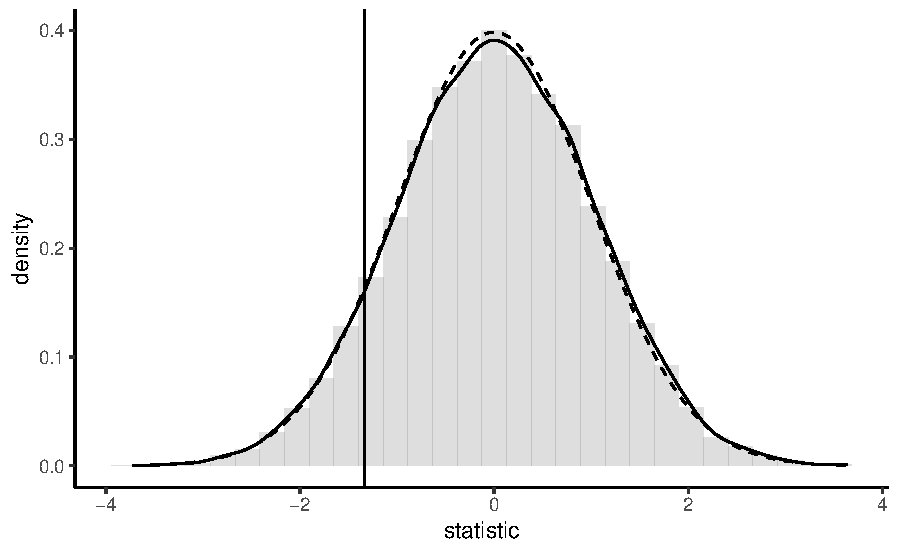
\includegraphics[width=0.85\textwidth,height=\textheight]{inference_files/figure-pdf/fig-renfepermut-1.pdf}

}

\caption{\label{fig-renfepermut}Permutation-based approximation to the
null distribution of Welch two-sample t-test statistic (histogram and
black curve) with standard normal approximation (dashed curve) for the
price of AVE tickets at promotional rate between Madrid and Barcelona.
The value of the test statistic calculated using the original sample is
represented by a vertical line.}

\end{figure}%

The so-called bootstrap approximation to the \emph{p}-value of the
permutation test, \(0.186,\) is the proportion of statistics that are
more extreme than the one based on the original sample. It is nearly
identical to that obtained from the Satterthwaite approximation,
\(0.249\) (the Student-\(t\) distribution is numerically equivalent to a
standard normal with that many degrees of freedom), as shown in
Figure~\ref{fig-renfepermut}. Even if our sample is very large
(\(n=8059\) observations), the difference is not statistically
significative. With a bigger sample (the database has more than 2
million tickets), we could estimate more precisely the average
difference, up to 1/100 of an euro: the price difference would
eventually become statistically significative, but this says nothing
about practical difference: \(0.28\) euros relative to an Promo ticket
priced on average \(82.56\) euros is a negligible amount.

\end{example}

\bookmarksetup{startatroot}

\chapter{Likelihood-based inference}\label{likelihood}

This chapter is dedicated to the basics of statistical modelling using
likelihood-based inference, arguably the most popular estimation
paradigm in statistics.

\begin{tcolorbox}[enhanced jigsaw, coltitle=black, colframe=quarto-callout-important-color-frame, breakable, opacityback=0, title=\textcolor{quarto-callout-important-color}{\faExclamation}\hspace{0.5em}{Important}, left=2mm, arc=.35mm, colbacktitle=quarto-callout-important-color!10!white, opacitybacktitle=0.6, titlerule=0mm, rightrule=.15mm, bottomtitle=1mm, toptitle=1mm, leftrule=.75mm, colback=white, toprule=.15mm, bottomrule=.15mm]

\textbf{Learning objectives}:

\begin{itemize}
\tightlist
\item
  Learn the terminology associated with likelihood-based inference
\item
  Derive closed-form expressions for the maximum likelihood estimator in
  simple models
\item
  Using numerical optimization, obtain parameter estimates and their
  standards errors using maximum likelihood
\item
  Use large-sample properties of the likelihood to derive confidence
  intervals and tests
\item
  Use information criteria for model selection
\end{itemize}

\end{tcolorbox}

A statistical model starts with the specification of a data generating
mechanism. We postulate that the data has been generated from a
probability distribution with \(p\)-dimensional parameter vector
\(\boldsymbol{\theta}.\) The sample space is the set in which the \(n\)
vector observations lie, while the parameter space
\(\boldsymbol{\Theta} \subseteq \mathbb{R}^p\) is the set in which the
parameter takes values.

As motivating example, consider the time a passenger must wait at the
\emph{Université de Montréal} station if that person arrives at 17:59
sharp every weekday, just in time for the metro train. The measurements
in \texttt{waiting} represent the time in seconds before the next train
leaves the station. The data were collected over three months and can be
treated as an independent sample. The left panel of
Figure~\ref{fig-waiting-hist} shows an histogram of the \(n=62\)
observations, which range from \(4\) to \(57\) seconds. The data are
positive, so our model must account for this feature.

\begin{figure}[ht!]

\centering{

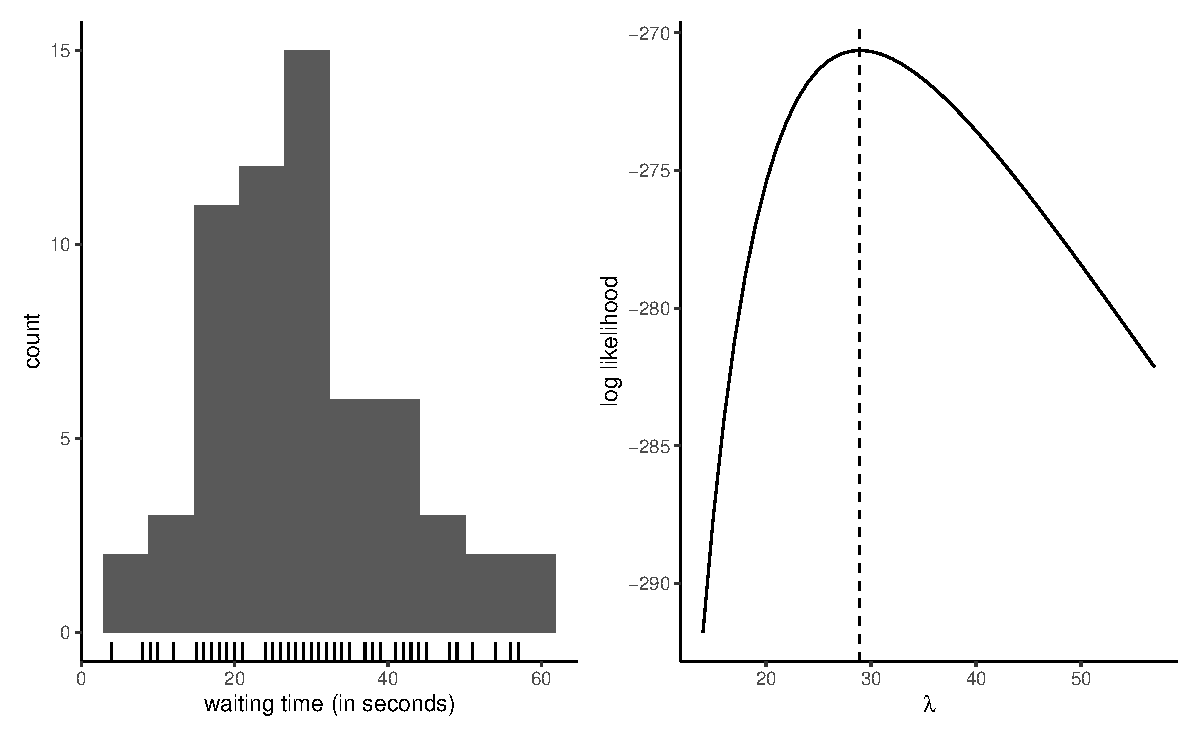
\includegraphics[width=0.85\textwidth,height=\textheight]{likelihood_files/figure-pdf/fig-waiting-hist-1.pdf}

}

\caption{\label{fig-waiting-hist}Histogram of waiting time with rugs for
the observations (left) and exponential log likelihood function for the
waiting time, with the maximum likelihood estimate at dashed vertical
line (right).}

\end{figure}%

\begin{example}[Exponential model for waiting
times]\protect\hypertarget{exm-exponential-model}{}\label{exm-exponential-model}

To model the waiting time, we may consider for example an exponential
distribution with scale \(\lambda\)
(Definition~\ref{def-exponentialdist}), which represents the theoretical
mean. Under independence\footnote{Recall that, if \(A\) and \(B\) are
  independent random variables, the joint probability is the product of
  the probability of the events, \(\Pr(A \cup B) = \Pr(A)\Pr(B).\) The
  same holds for density or mass function, since the latter are defined
  as the derivative of the distribution function.}, the joint density
for the observations \(y_1, \ldots, y_n\) is \begin{align*}
f(\boldsymbol{y}) = \prod_{i=1}^n f(y_i) =\prod_{i=1}^n  \lambda^{-1} \exp(- y_i/\lambda) = \lambda^{-n} \exp\left(- \sum_{i=1}^n y_i/\lambda\right)
\end{align*} The sample space is \(\mathbb{R}_{+}^n = [0, \infty)^n,\)
while the parameter space is \((0, \infty).\)

\end{example}

To estimate the scale parameter \(\lambda\) and obtain suitable
uncertainty measures, we need a modelling framework. We turn to
likelihood-based inference.

\section{Maximum likelihood
estimation}\label{maximum-likelihood-estimation}

For any given value of \(\boldsymbol{\theta},\) we can obtain the
probability mass or density of the sample observations, and we use this
to derive an objective function for the estimation.

\begin{definition}[Likelihood]\protect\hypertarget{def-likelihood}{}\label{def-likelihood}

The \textbf{likelihood} \(L(\boldsymbol{\theta})\) is a function of the
parameter vector \(\boldsymbol{\theta}\) that gives the probability (or
density) of observing a sample under a postulated distribution, treating
the observations as fixed, \begin{align*}
L(\boldsymbol{\theta}; \boldsymbol{y}) = f(\boldsymbol{y}; \boldsymbol{\theta}),
\end{align*} where \(f(\boldsymbol{y}; \boldsymbol{\theta})\) denotes
the joint density or mass function of the \(n\)-vector containing the
observations.

If the latter are independent, the joint density factorizes as the
product of the density of individual observations, and the likelihood
becomes \begin{align*}
L(\boldsymbol{\theta}; \boldsymbol{y})=\prod_{i=1}^n f_i(y_i; \boldsymbol{\theta}) = f_1(y_1; \boldsymbol{\theta}) \times \cdots \times f_n(y_n; \boldsymbol{\theta}).
\end{align*} The corresponding log likelihood function for independent
and identically distributions observations is \begin{align*}
\ell(\boldsymbol{\theta}; \boldsymbol{y}) = \sum_{i=1}^n \ln f(y_i; \boldsymbol{\theta})
\end{align*}

\end{definition}

\begin{example}[Dependent
data]\protect\hypertarget{exm-markov}{}\label{exm-markov}

The joint density function only factorizes for independent data, but an
alternative sequential decomposition can be helpful. For example, we can
write the joint density \(f(y_1, \ldots, y_n)\) using the factorization
\begin{align*}
f(\boldsymbol{y}) = f(y_1) \times f(y_2 \mid y_1) \times \ldots f(y_n \mid y_1, \ldots, y_n)
\end{align*} in terms of conditional. Such a decomposition is
particularly useful in the context of time series, where data are
ordered from time \(1\) until time \(n\) and models typically relate
observation \(y_n\) to it's past. For example, the \(\mathsf{AR}(1)\)
process, states that
\(Y_t \mid Y_{t-1}=y_{t-1} \sim \mathsf{normal}(\alpha + \beta y_{t-1}, \sigma^2)\)
and we can simplify the log likelihood using the Markov property, which
states that the current realization depends on the past,
\(Y_t \mid Y_1, \ldots, Y_{t-1},\) only through the most recent value
\(Y_{t-1}.\) The log likelihood thus becomes \begin{align*}
\ell(\boldsymbol{\theta}) = \ln f(y_1) + \sum_{i=2}^n f(y_i \mid y_{i-1}).
\end{align*}

\end{example}

\begin{definition}[Maximum likelihood
estimator]\protect\hypertarget{def-mle}{}\label{def-mle}

The \textbf{maximum likelihood estimator}
\(\widehat{\boldsymbol{\theta}}\) is the vector value that maximizes the
likelihood, \begin{align*}
\widehat{\boldsymbol{\theta}} = \mathrm{arg max}_{\boldsymbol{\theta} \in \boldsymbol{\Theta}} L(\boldsymbol{\theta}; \boldsymbol{y}).
\end{align*}

The natural logarithm \(\ln\) is a monotonic transformation, so the
maximum likelihood estimator \(\boldsymbol{\theta}\) for likelihood
\(L(\boldsymbol{\theta}; \boldsymbol{y})\) is the same as that of the
log likelihood
\(\ell(\boldsymbol{\theta}; \boldsymbol{y}) = \ln L(\boldsymbol{\theta}; \boldsymbol{y}).\)\footnote{Since
  in most instances we deal with a product of densities, taking the log
  leads to a sum of log density contributions, which facilitates
  optimization.}

\end{definition}

If we suppose that our model is correct, than we expect to observe
whatever was realized, so we find the parameter vector that makes the
sample the most likely to have been generated by our model. Several
properties of maximum likelihood estimator makes it appealing for
inference. The maximum likelihood estimator is efficient, meaning it has
the smallest asymptotic mean squared error. The maximum likelihood
estimator is also \textbf{consistent}, i.e., it converges to the correct
value as the sample size increase (asymptotically unbiased).

We can resort to numerical optimization routines to find the value of
the maximum likelihood estimate, or sometimes derive closed-form
expressions for the estimator, starting from the log likelihood. The
right panel of Figure~\ref{fig-waiting-hist} shows the exponential log
likelihood, which attains a maximum at \(\widehat{\lambda}=28.935\)
second, the sample mean of the observations. The function decreases to
either side of these values as the data become less compatible with the
model. Given the values achieved here with a small sample, it is easy to
see that direct optimization of the likelihood function (rather than
it's natural logarithm) could lead to numerical underflow, since already
\(\exp(-270) \approx 5.5 \times 10^{-118},\) and log values smaller than
\(-746\) would be rounded to zero.

\begin{example}[Calculation of the maximum likelihood of an exponential
distribution]\protect\hypertarget{exm-exponential-mle}{}\label{exm-exponential-mle}

As Figure~\ref{fig-waiting-hist} reveals that the exponential log
likelihood function is unimodal and thus achieves a single maximum, we
can use calculus to derive an explicit expression for
\(\widehat{\lambda}\) based on the log likelihood \begin{align*}
\ell(\lambda) = -n \ln\lambda -\frac{1}{\lambda} \sum_{i=1}^n y_i.
\end{align*} Taking first derivative and setting the result to zero, we
find \begin{align*}
\frac{\mathrm{d} \ell(\lambda)}{\mathrm{d} \lambda}  = -\frac{n}{\lambda} + \frac{1}{\lambda^2} \sum_{i=1}^n y_i = 0.
\end{align*} Rearranging this expression by taking \(-n/\lambda\) to the
right hand side of the equality and multiplying both sides by
\(\lambda^2>0,\) we find that
\(\widehat{\lambda} = \sum_{i=1}^n y_i / n.\) The second derivative of
the log likelihood is
\(\mathrm{d}^2 \ell(\lambda)/\mathrm{d} \lambda^2 = n(\lambda^{-2} - 2\lambda^{-3}\overline{y}),\)
and plugging \(\lambda = \overline{y}\) gives \(-n/\overline{y}^2,\)
which is negative. Therefore, \(\widehat{\lambda}\) is indeed a
maximizer.

\end{example}

\begin{example}[Normal
samples]\protect\hypertarget{exm-normal-mle}{}\label{exm-normal-mle}

Suppose we have an independent normal sample of size \(n\) with mean
\(\mu\) and variance \(\sigma^2\), where
\(Y_i \sim \mathsf{normal}(\mu, \sigma^2)\) are independent. Recall that
the density of the normal distribution is \begin{align*}
f(y; \mu, \sigma^2)=\frac{1}{(2\pi \sigma^2)^{1/2}}\exp\left\{-\frac{1}{2\sigma^2}(x-\mu)^2\right\}.
\end{align*} For an simple random sample of size \(n\), whose
realization is \(y_1, \ldots, y_n\), the likelihood is \begin{align*}
L(\mu, \sigma^2; \boldsymbol{y})=&\prod_{i=1}^n\frac{1}{({2\pi \sigma^2})^{1/2}}\exp\left\{-\frac{1}{2\sigma^2}(y_i-\mu)^2\right\}\\
=&(2\pi \sigma^2)^{-n/2}\exp\left\{-\frac{1}{2\sigma^2}\sum_{i=1}^n(y_i-\mu)^2\right\}.
\end{align*} and the log likelihood is \begin{align*}
\ell(\mu, \sigma^2; \boldsymbol{y})=-\frac{n}{2}\ln(2\pi) -\frac{n}{2}\ln(\sigma^2)-\frac{1}{2\sigma^2}\sum_{i=1}^n (y_i-\mu)^2.
\end{align*}

One can show that the maximum likelihood estimators for the two
parameters are \begin{align*}
\widehat{\mu}=\overline{Y}=\frac{1}{n} \sum_{i=1}^n Y_i, \qquad \widehat{\sigma}^2=\frac{1}{n}\sum_{i=1}^n (Y_i-\overline{Y})^2.
\end{align*}

The fact that the estimator of the theoretical mean \(\mu\) is the
sample mean is fairly intuitive and one can show the estimator is
unbiased for \(\mu\). The (unbiased) sample variance estimator,
\begin{align*}
S^2=\frac{1}{n-1} \sum_{i=1}^n (Y_i-\overline{Y})^2
\end{align*} Since \(\widehat{\sigma}^2=(n-1)/n S^2\), it follows that
the maximum likelihood estimator of \(\sigma^2\) is biased, but both
estimators are consistent and will thus get arbitrarily close to the
true value \(\sigma^2\) for \(n\) sufficiently large.

\end{example}

\begin{proposition}[Invariance of maximum likelihood
estimators]\protect\hypertarget{prp-invariance-mle}{}\label{prp-invariance-mle}

If \(g(\boldsymbol{\theta}): \mathbb{R}^p \mapsto \mathbb{R}^k\) for
\(k \leq p\) is a function of the parameter vector, then
\(g(\widehat{\boldsymbol{\theta}})\) is the maximum likelihood estimator
of the function.

\end{proposition}

The invariance property explains the widespread use of maximum
likelihood estimation. For example, having estimated the parameter
\(\lambda,\) we can now use the model to derive other quantities of
interest and get the ``best'' estimates for free. For example, we could
compute the maximum likelihood estimate of the probability of waiting
more than one minute,
\(\Pr(T>60) = \exp(-60/\widehat{\lambda})= 0.126,\) or using \textbf{R}
built-in distribution function \texttt{pexp}.

\begin{Shaded}
\begin{Highlighting}[]
\CommentTok{\# Note: default R parametrization for the exponential is }
\CommentTok{\# in terms of rate, i.e., the inverse scale parameter}
\FunctionTok{pexp}\NormalTok{(}\AttributeTok{q =} \DecValTok{60}\NormalTok{, }\AttributeTok{rate =} \DecValTok{1}\SpecialCharTok{/}\FunctionTok{mean}\NormalTok{(waiting), }\AttributeTok{lower.tail =} \ConstantTok{FALSE}\NormalTok{)}
\CommentTok{\#\textgreater{} [1] 0.126}
\end{Highlighting}
\end{Shaded}

Another appeal of the invariance property is the possibility to compute
the MLE in the most suitable parametrization, which is convenient if the
support is restricted. If \(g\) is a one-to-one function of
\(\boldsymbol{\theta},\) for example if \(\theta >0,\) taking
\(g(\theta) = \ln \theta\) or, if \(0 \leq \theta \leq 1,\) by
maximizing \(g(\theta) = \ln(\theta) - \ln(1-\theta) \in \mathbb{R}\)
removes the support constraints for the numerical optimization.

\begin{definition}[Score and information
matrix]\protect\hypertarget{def-information}{}\label{def-information}

Let \(\ell(\boldsymbol{\theta}),\)
\(\boldsymbol{\theta} \in \boldsymbol{\Theta} \subseteq \mathbb{R}^p,\)
be the log likelihood function. The gradient of the log likelihood
\(U(\boldsymbol{\theta}) = \partial \ell(\boldsymbol{\theta}) / \partial \boldsymbol{\theta}\)
is termed \textbf{score} function.

The \textbf{observed information matrix} is the hessian of the negative
log likelihood \begin{align*}
j(\boldsymbol{\theta}; \boldsymbol{y})=-\frac{\partial^2 \ell(\boldsymbol{\theta}; \boldsymbol{y})}{\partial \boldsymbol{\theta} \partial \boldsymbol{\theta}^\top},
\end{align*} evaluated at the maximum likelihood estimate
\(\widehat{\boldsymbol{\theta}},\) so
\(j(\widehat{\boldsymbol{\theta}}).\) Under regularity conditions, the
\textbf{expected information}, also called \textbf{Fisher information}
matrix, is \begin{align*}
i(\boldsymbol{\theta}) = \mathsf{E}\left\{U(\boldsymbol{\theta}; \boldsymbol{Y}) U(\boldsymbol{\theta}; \boldsymbol{Y})^\top\right\} = \mathsf{E}\left\{j(\boldsymbol{\theta}; \boldsymbol{Y})\right\}
\end{align*} Both the Fisher (or expected) and the observed information
matrices are symmetric and encode the curvature of the log likelihood
and provide information about the variability of
\(\widehat{\boldsymbol{\theta}}.\)

\end{definition}

\begin{example}[Information for the exponential
model]\protect\hypertarget{exm-exponential}{}\label{exm-exponential}

The observed and expected information of the exponential model for a
random sample \(Y_1, \ldots, Y_n,\) parametrized in terms of scale
\(\lambda,\) are \begin{align*}
j(\lambda; \boldsymbol{y}) &= -\frac{\partial^2 \ell(\lambda)}{\partial \lambda^2} = \frac{n}{\lambda^{2}} + \frac{2}{n\lambda^{3}}\sum_{i=1}^n y_i \\
i(\lambda) &= \frac{n}{\lambda^{2}} + \frac{2}{n\lambda^{3}}\sum_{i=1}^n \mathsf{E}(Y_i)  = \frac{n}{\lambda^{2}}
\end{align*} since \(\mathsf{E}(Y_i) = \lambda\) and expectation is a
linear operator.

We find
\(i(\widehat{\lambda}) = j(\widehat{\lambda}) = n/\overline{y}^2\).

\end{example}

The exponential model may be restrictive for our purposes, so we
consider for the purpose of illustration and as a generalization a
Weibull distribution.

\begin{definition}[Weibull
distribution]\protect\hypertarget{def-weibull}{}\label{def-weibull}

The distribution function of a \textbf{Weibull} random variable with
scale \(\lambda>0\) and shape \(\alpha>0\) is \begin{align*}
F(x; \lambda, \alpha) &= 1 - \exp\left\{-(x/\lambda)^\alpha\right\}, \qquad x \geq 0, \lambda>0, \alpha>0,
\end{align*} while the corresponding density is \begin{align*}
f(x; \lambda, \alpha) &= \frac{\alpha}{\lambda^\alpha} x^{\alpha-1}\exp\left\{-(x/\lambda)^\alpha\right\}, \qquad x \geq 0, \lambda>0, \alpha>0.
\end{align*} The quantile function, the inverse of the distribution
function, is \(Q(p) = \lambda\{-\ln(1-p)\}^{1/\alpha}.\) The Weibull
distribution includes the exponential as special case when \(\alpha=1.\)
The expected value of \(Y \sim \mathsf{Weibull}(\lambda, \alpha)\) is
\(\mathsf{E}(Y) = \lambda \Gamma(1+1/\alpha).\)

\end{definition}

\begin{example}[Score and information of the Weibull
distribution]\protect\hypertarget{exm-weibull-info}{}\label{exm-weibull-info}

The log likelihood for a simple random sample whose realizations are
\(y_1, \ldots, y_n\) of size \(n\) from a
\(\mathsf{Weibull}(\lambda, \alpha)\) model is \begin{align*}
\ell(\lambda, \alpha) = n \ln(\alpha) - n\alpha\ln(\lambda) + (\alpha-1) \sum_{i=1}^n \ln y_i  - \lambda^{-\alpha}\sum_{i=1}^n y_i^\alpha.
\end{align*} The score, which is the gradient of the log likelihood, is
easily obtained by differentiation\footnote{Using for example a symbolic
  calculator.} \begin{align*}
U(\lambda, \alpha) = \begin{pmatrix}\frac{\partial \ell(\lambda, \alpha)}{\partial \lambda} \\
\frac{\partial \ell(\lambda, \alpha)}{\partial \alpha} \end{pmatrix} &= 
\begin{pmatrix}
 -\frac{n\alpha}{\lambda} +\alpha\lambda^{-\alpha-1}\sum_{i=1}^n y_i^\alpha
 \\
 \frac{n}{\alpha} - n \ln(\lambda) + \sum_{i=1}^n \ln y_i  - \sum_{i=1}^n \left(\frac{y_i}{\lambda}\right)^{\alpha} \times\ln\left(\frac{y_i}{\lambda}\right).
 \end{pmatrix}
\end{align*} and the observed information is the \(2 \times 2\)
matrix-valued function \begin{align*}
j(\lambda, \alpha) &= - \begin{pmatrix}
\frac{\partial^2 \ell(\lambda, \alpha)}{\partial \lambda^2} &  \frac{\partial^2 \ell(\lambda, \alpha)}{\partial \lambda \partial \alpha} \\ \frac{\partial^2 \ell(\lambda, \alpha)}{\partial \alpha \partial \lambda} & \frac{\partial^2 \ell(\lambda, \alpha)}{\partial \alpha^2}
\end{pmatrix} 
\\&= \begin{pmatrix}
\lambda^{-2}\left\{-n\alpha + \alpha(\alpha+1)\sum_{i=1}^n (y_i/\lambda)^2\right\} & \lambda^{-1}\sum_{i=1}^n [1-(y_i/\lambda)^\alpha\{1+\alpha\ln(y_i/\lambda)\}]\\ \lambda^{-1}\sum_{i=1}^n [1-(y_i/\lambda)^\alpha\{1+\alpha\ln(y_i/\lambda)\}]& n\alpha^{-2} + \sum_{i=1}^n (y_i/\lambda)^\alpha \{\ln(y_i/\theta)\}^2
\end{pmatrix}
\end{align*}

\end{example}

\begin{proposition}[Gradient-based
optimization]\protect\hypertarget{prp-gradient}{}\label{prp-gradient}

To obtain the maximum likelihood estimator, we will typically find the
value of the vector \(\boldsymbol{\theta}\) that solves the score
vector, meaning \(U(\widehat{\boldsymbol{\theta}})=\boldsymbol{0}_p.\)
This amounts to solving simultaneously a \(p\)-system of equations by
setting the derivative with respect to each element of
\(\boldsymbol{\theta}\) to zero. If \(j(\widehat{\boldsymbol{\theta}})\)
is a positive definite matrix (i.e., all of it's eigenvalues are
positive), then the vector \(\widehat{\boldsymbol{\theta}}\) is the
maximum likelihood estimator.

We can use a variant of Newton--Raphson algorithm if the likelihood is
thrice differentiable and the maximum likelihood estimator does not lie
on the boundary of the parameter space. If we consider an initial value
\(\boldsymbol{\theta}^{\dagger},\) then a first order Taylor series
expansion of the score likelihood in a neighborhood
\(\boldsymbol{\theta}^{\dagger}\) of the MLE
\(\widehat{\boldsymbol{\theta}}\) gives \begin{align*}
\boldsymbol{0}_p & = U(\widehat{\boldsymbol{\theta}}) \stackrel{\cdot}{\simeq} \left.
\frac{\partial \ell(\boldsymbol{\theta})}{\partial \boldsymbol{\theta}} \right|_{\boldsymbol{\theta} = \boldsymbol{\theta}^{\dagger}} + \left.
\frac{\partial^2 \ell(\boldsymbol{\theta})}{\partial \boldsymbol{\theta} \partial \boldsymbol{\theta}^\top}\right|_{\boldsymbol{\theta} = \boldsymbol{\theta}^{\dagger}}(\widehat{\boldsymbol{\theta}} - \boldsymbol{\theta}^{\dagger})\\&=U(\boldsymbol{\theta}^{\dagger}) - j(\boldsymbol{\theta}^{\dagger})(\widehat{\boldsymbol{\theta}} - \boldsymbol{\theta}^{\dagger})
\end{align*} and solving this for \(\widehat{\boldsymbol{\theta}}\)
(provided the \(p \times p\) matrix \(j(\widehat{\boldsymbol{\theta}})\)
is invertible), we get \begin{align*}
\widehat{\boldsymbol{\theta}} \stackrel{\cdot}{\simeq} \boldsymbol{\theta}^{\dagger} + 
j^{-1}(\boldsymbol{\theta}^{\dagger})U(\boldsymbol{\theta}^{\dagger}),
\end{align*} which suggests an iterative procedure from a starting value
\(\boldsymbol{\theta}^{\dagger}\) in the vicinity of the mode until the
gradient is approximately zero. If the value is far from the mode, then
the algorithm may diverge to infinity. To avoid this, we may multiply
the term
\(j^{-1}(\boldsymbol{\theta}^{\dagger})U(\boldsymbol{\theta}^{\dagger})\)
by a damping factor \(c<1.\) A variant of the algorithm, termed Fisher
scoring, uses the expected or Fisher information
\(i(\boldsymbol{\theta})\) in place of the observed information,
\(j(\boldsymbol{\theta}),\) for numerical stability and to avoid
situations where the latter is not positive definite. This is the
optimization routine used in the \texttt{glm} function in \textbf{R}.

\end{proposition}

\begin{example}[Maximum likelihood of a Weibull
sample]\protect\hypertarget{exm-weibull-mle}{}\label{exm-weibull-mle}

We turn to numerical optimization to obtain the maximum likelihood
estimate of the Weibull distribution, in the absence of closed-form
expression for the MLE. To this end, we create functions that encode the
log likelihood, here taken as the sum of log density contributions. The
function \texttt{nll\_weibull} below takes as argument the vector of
parameters, \texttt{pars}, and returns the negative of the log
likelihood which we wish to minimize\footnote{Most optimization
  algorithms minimize functions with respect to their arguments, so we
  minimize the negative log likelihood, which is equivalent to
  maximizing the log likelihood.} We also code the gradient, although we
can resort to numerical differentiation at little additional costs. We
then use \texttt{optim}, the default optimization routine in \textbf{R},
to minimize \texttt{nll\_weibull}. The function returns a list
containing a convergence code (\texttt{0} indicating convergence), the
MLE in \texttt{par}, the log likelihood
\(\ell(\widehat{\boldsymbol{\theta}})\) and the Hessian matrix, which is
the matrix of second derivatives of the negative log likelihood
evaluated at \(\widehat{\boldsymbol{\theta}}.\) The log likelihood
surface, for pairs of scale and shape vectors
\(\boldsymbol{\theta} = (\lambda, \alpha),\) are displayed in
Figure~\ref{fig-weibull-profile}. We can see that the maximum likelihood
value has converged, and check that the score satisfies
\(U(\widehat{\boldsymbol{\theta}}) = 0\) at the returned optimum value.

\begin{Shaded}
\begin{Highlighting}[]
\CommentTok{\# Load data vector}
\FunctionTok{data}\NormalTok{(waiting, }\AttributeTok{package =} \StringTok{"hecstatmod"}\NormalTok{)}
\CommentTok{\# Negative log likelihood for a Weibull sample}
\NormalTok{nll\_weibull }\OtherTok{\textless{}{-}} \ControlFlowTok{function}\NormalTok{(pars, y)\{}
  \CommentTok{\# Handle the case of negative parameter values}
  \ControlFlowTok{if}\NormalTok{(}\FunctionTok{isTRUE}\NormalTok{(}\FunctionTok{any}\NormalTok{(pars }\SpecialCharTok{\textless{}=} \DecValTok{0}\NormalTok{)))\{ }\CommentTok{\# parameters must be positive}
    \FunctionTok{return}\NormalTok{(}\FloatTok{1e10}\NormalTok{) }\CommentTok{\# large value (not infinite, to avoid warning messages)}
\NormalTok{  \}}
  \SpecialCharTok{{-}} \FunctionTok{sum}\NormalTok{(}\FunctionTok{dweibull}\NormalTok{(}\AttributeTok{x =}\NormalTok{ y, }\AttributeTok{scale =}\NormalTok{ pars[}\DecValTok{1}\NormalTok{], }\AttributeTok{shape =}\NormalTok{ pars[}\DecValTok{2}\NormalTok{], }\AttributeTok{log =} \ConstantTok{TRUE}\NormalTok{))}
\NormalTok{\}}
\CommentTok{\# Gradient of the negative Weibull log likelihood}
\NormalTok{gr\_nll\_weibull }\OtherTok{\textless{}{-}} \ControlFlowTok{function}\NormalTok{(pars, y)\{}
\NormalTok{  scale }\OtherTok{\textless{}{-}}\NormalTok{ pars[}\DecValTok{1}\NormalTok{] }
\NormalTok{  shape }\OtherTok{\textless{}{-}}\NormalTok{ pars[}\DecValTok{2}\NormalTok{]}
\NormalTok{  n }\OtherTok{\textless{}{-}} \FunctionTok{length}\NormalTok{(y)}
\NormalTok{  grad\_ll }\OtherTok{\textless{}{-}} \FunctionTok{c}\NormalTok{(}\AttributeTok{scale =} \SpecialCharTok{{-}}\NormalTok{n}\SpecialCharTok{*}\NormalTok{shape}\SpecialCharTok{/}\NormalTok{scale }\SpecialCharTok{+}\NormalTok{ shape}\SpecialCharTok{*}\NormalTok{scale}\SpecialCharTok{\^{}}\NormalTok{(}\SpecialCharTok{{-}}\NormalTok{shape}\DecValTok{{-}1}\NormalTok{)}\SpecialCharTok{*}\FunctionTok{sum}\NormalTok{(y}\SpecialCharTok{\^{}}\NormalTok{shape),}
               \AttributeTok{shape =}\NormalTok{ n}\SpecialCharTok{/}\NormalTok{shape }\SpecialCharTok{{-}}\NormalTok{ n}\SpecialCharTok{*}\FunctionTok{log}\NormalTok{(scale) }\SpecialCharTok{+} \FunctionTok{sum}\NormalTok{(}\FunctionTok{log}\NormalTok{(y)) }\SpecialCharTok{{-}} 
                 \FunctionTok{sum}\NormalTok{(}\FunctionTok{log}\NormalTok{(y}\SpecialCharTok{/}\NormalTok{scale)}\SpecialCharTok{*}\NormalTok{(y}\SpecialCharTok{/}\NormalTok{scale)}\SpecialCharTok{\^{}}\NormalTok{shape))}
  \FunctionTok{return}\NormalTok{(}\SpecialCharTok{{-}}\NormalTok{ grad\_ll)}
\NormalTok{\}}
\CommentTok{\# Use exponential submodel MLE as starting parameters}
\NormalTok{start }\OtherTok{\textless{}{-}} \FunctionTok{c}\NormalTok{(}\FunctionTok{mean}\NormalTok{(waiting), }\DecValTok{1}\NormalTok{)}
\CommentTok{\# Check gradient function is correctly coded! }
\CommentTok{\# Returns TRUE if numerically equal to tolerance}
\FunctionTok{isTRUE}\NormalTok{(}\FunctionTok{all.equal}\NormalTok{(numDeriv}\SpecialCharTok{::}\FunctionTok{grad}\NormalTok{(nll\_weibull, }\AttributeTok{x =}\NormalTok{ start, }\AttributeTok{y =}\NormalTok{ waiting),}
                 \FunctionTok{gr\_nll\_weibull}\NormalTok{(}\AttributeTok{pars =}\NormalTok{ start, }\AttributeTok{y =}\NormalTok{ waiting),}
                 \AttributeTok{check.attributes =} \ConstantTok{FALSE}\NormalTok{))}
\CommentTok{\#\textgreater{} [1] TRUE}
\CommentTok{\# Numerical minimization using optim}
\NormalTok{opt\_weibull }\OtherTok{\textless{}{-}} \FunctionTok{optim}\NormalTok{(}
  \AttributeTok{par =}\NormalTok{ start,  }\CommentTok{\# starting values}
  \AttributeTok{fn =}\NormalTok{ nll\_weibull,  }\CommentTok{\# pass function, whose first argument is the parameter vector}
  \AttributeTok{gr =}\NormalTok{ gr\_nll\_weibull, }\CommentTok{\# optional (if missing, numerical derivative)}
  \AttributeTok{method =} \StringTok{"BFGS"}\NormalTok{, }\CommentTok{\# gradient{-}based algorithm, common alternative is "Nelder"}
  \AttributeTok{y =}\NormalTok{ waiting, }\CommentTok{\# vector of observations, passed as additional argument to fn}
  \AttributeTok{hessian =} \ConstantTok{TRUE}\NormalTok{) }\CommentTok{\# return matrix of second derivatives evaluated at MLE}
\CommentTok{\# Alternative using pure Newton}
\CommentTok{\# nlm(f = nll\_weibull, p = start, hessian = TRUE, y = waiting)}
\CommentTok{\# Parameter estimates {-} MLE}
\NormalTok{(mle\_weibull }\OtherTok{\textless{}{-}}\NormalTok{ opt\_weibull}\SpecialCharTok{$}\NormalTok{par)}
\CommentTok{\#\textgreater{} [1] 32.6  2.6}
\CommentTok{\# Check gradient for convergence}
\FunctionTok{gr\_nll\_weibull}\NormalTok{(mle\_weibull, }\AttributeTok{y =}\NormalTok{ waiting)}
\CommentTok{\#\textgreater{}     scale     shape }
\CommentTok{\#\textgreater{} 0.0000142 0.0001136}
\CommentTok{\# Is the Hessian of the negative positive definite (all eigenvalues are positive)}
\CommentTok{\# If so, we found a maximum and the matrix is invertible}
\FunctionTok{isTRUE}\NormalTok{(}\FunctionTok{all}\NormalTok{(}\FunctionTok{eigen}\NormalTok{(opt\_weibull}\SpecialCharTok{$}\NormalTok{hessian)}\SpecialCharTok{$}\NormalTok{values }\SpecialCharTok{\textgreater{}} \DecValTok{0}\NormalTok{))}
\CommentTok{\#\textgreater{} [1] TRUE}
\end{Highlighting}
\end{Shaded}

\end{example}

\section{Sampling distribution}\label{sampling-distribution}

The \textbf{sampling distribution} of an estimator
\(\widehat{\boldsymbol{\theta}}\) is the probability distribution
induced by the underlying data, given that the latter inputs are random.

For simplicity, suppose we have a simple random sample, so the log
likelihood is a sum of \(n\) terms and information accumulates linearly
with the sample size: the data carry more information about the unknown
parameter vector, whose true value we denote \(\boldsymbol{\theta}_0.\)
Under suitable regularity conditions, cf.~Section 4.4.2 of Davison
(\citeproc{ref-Davison:2003}{2003}), for large sample size \(n,\) we can
perform a Taylor series of the score vector and apply the central limit
theorem. Since \(U(\boldsymbol{\theta})\) and \(i(\boldsymbol{\theta})\)
are the sum of \(n\) independent random variables, and that
\(\mathsf{E}\{U(\boldsymbol{\theta})\}=\boldsymbol{0}_p,\) and
\(\mathsf{Var}\{U(\boldsymbol{\theta})\}=i(\boldsymbol{\theta}),\)
application of the central limit theorem yields \begin{align*}
i(\boldsymbol{\theta}_0)^{-1/2}U(\boldsymbol{\theta}_0) \stackrel{\cdot}{\sim}\mathsf{normal}_p(\boldsymbol{0}, \mathbf{I}_p).
\end{align*}

We can use this to obtain approximations to the sampling distribution of
\(\widehat{\boldsymbol{\theta}},\) given that \begin{align*}
\widehat{\boldsymbol{\theta}} \stackrel{\cdot}{\sim} \mathsf{normal}_p\{\boldsymbol{\theta}_0, i^{-1}(\boldsymbol{\theta})\}
\end{align*} where the covariance matrix is the inverse of the Fisher
information. In practice, since the true parameter value
\(\boldsymbol{\theta}_0\) is unknown, we replace it with either
\(i^{-1}(\widehat{\boldsymbol{\theta}})\) or the inverse of the observed
information \(j^{-1}(\widehat{\boldsymbol{\theta}}),\) as both of these
converge to the true value.

As the sample size grows, the \(\widehat{\boldsymbol{\theta}}\) becomes
centered around the value \(\boldsymbol{\theta}_0\) that minimizes the
discrepancy between the model and the true data generating process. In
large samples, the sampling distribution of the maximum likelihood
estimator is approximately quadratic.

\begin{example}[Covariance matrix and standard errors for the Weibull
distribution]\protect\hypertarget{exm-Weibull-se}{}\label{exm-Weibull-se}

We use the output of our optimization procedure to get the observed
information matrix and the standard errors for the parameters of the
Weibull model. The latter are simply the square root of the diagonal
entries of the inverse Hessian matrix,
\([\mathrm{diag}\{j^{-1}(\widehat{\boldsymbol{\theta}})\}]^{1/2}\).

\begin{Shaded}
\begin{Highlighting}[]
\CommentTok{\# The Hessian matrix of the negative log likelihood}
\CommentTok{\# evaluated at the MLE (observed information matrix)}
\NormalTok{obsinfo\_weibull }\OtherTok{\textless{}{-}}\NormalTok{ opt\_weibull}\SpecialCharTok{$}\NormalTok{hessian}
\NormalTok{vmat\_weibull }\OtherTok{\textless{}{-}} \FunctionTok{solve}\NormalTok{(obsinfo\_weibull)}
\CommentTok{\# Standard errors}
\NormalTok{se\_weibull }\OtherTok{\textless{}{-}} \FunctionTok{sqrt}\NormalTok{(}\FunctionTok{diag}\NormalTok{(vmat\_weibull))}
\end{Highlighting}
\end{Shaded}

\end{example}

From these, one can readily Wald-based confidence intervals for
parameters from \(\boldsymbol{\theta}.\)

\begin{proposition}[Asymptotic normality and
transformations]\protect\hypertarget{prp-transformation}{}\label{prp-transformation}

The asymptotic normality result can be used to derive standard errors
for other quantities of interest. If \(\phi = g(\boldsymbol{\theta})\)
is a differentiable function of \(\boldsymbol{\theta}\) whose gradient
does not vanish at \(\widehat{\boldsymbol{\theta}}\) then
\(\widehat{\phi} \stackrel{\cdot}{\sim}\mathsf{normal}(\phi_0, \mathrm{V}_\phi),\)
with
\(\mathrm{V}_\phi = \nabla \phi^\top \mathbf{V}_{\boldsymbol{\theta}} \nabla \phi,\)
where
\(\nabla \phi=[\partial \phi/\partial \theta_1, \ldots, \partial \phi/\partial \theta_p]^\top.\)
The variance matrix and the gradient are evaluated at the maximum
likelihood estimate \(\widehat{\boldsymbol{\theta}}.\) This result
readily extends to vector \(\boldsymbol{\phi} \in \mathbb{R}^k\) for
\(k \leq p,\) where \(\mathrm{V}_\phi\)is the Jacobian matrix of the
transformation.

\end{proposition}

\begin{example}[Probability of waiting for exponential
model.]\protect\hypertarget{exm-transformation-exp}{}\label{exm-transformation-exp}

To illustrate the difference between likelihood ratio and Wald tests
(and their respective confidence intervals), we consider the metro
waiting time data and consider the probability of waiting more than one
minute, \(\phi=g(\lambda) = \exp(-60/\lambda).\) The maximum likelihood
estimate is, by invariance, \(0.126\) and the gradient of \(g\) with
respect to the scale parameter is
\(\nabla \phi = \partial \phi / \partial \lambda = 60\exp(-60/\lambda)/\lambda^2.\)

\begin{Shaded}
\begin{Highlighting}[]
\NormalTok{lambda\_hat }\OtherTok{\textless{}{-}} \FunctionTok{mean}\NormalTok{(waiting)}
\NormalTok{phi\_hat }\OtherTok{\textless{}{-}} \FunctionTok{exp}\NormalTok{(}\SpecialCharTok{{-}}\DecValTok{60}\SpecialCharTok{/}\NormalTok{lambda\_hat)}
\NormalTok{dphi }\OtherTok{\textless{}{-}} \ControlFlowTok{function}\NormalTok{(lambda)\{}\DecValTok{60}\SpecialCharTok{*}\FunctionTok{exp}\NormalTok{(}\SpecialCharTok{{-}}\DecValTok{60}\SpecialCharTok{/}\NormalTok{lambda)}\SpecialCharTok{/}\NormalTok{(lambda}\SpecialCharTok{\^{}}\DecValTok{2}\NormalTok{)\}}
\NormalTok{V\_lambda }\OtherTok{\textless{}{-}}\NormalTok{ lambda\_hat}\SpecialCharTok{\^{}}\DecValTok{2}\SpecialCharTok{/}\FunctionTok{length}\NormalTok{(waiting)}
\NormalTok{V\_phi }\OtherTok{\textless{}{-}} \FunctionTok{dphi}\NormalTok{(lambda\_hat)}\SpecialCharTok{\^{}}\DecValTok{2} \SpecialCharTok{*}\NormalTok{ V\_lambda}
\NormalTok{(se\_phi }\OtherTok{\textless{}{-}} \FunctionTok{sqrt}\NormalTok{(V\_phi))}
\CommentTok{\#\textgreater{} [1] 0.0331}
\end{Highlighting}
\end{Shaded}

\end{example}

\section{Likelihood-based tests}\label{liktests}

We consider a null hypothesis \(\mathscr{H}_0\) that imposes
restrictions on the possible values of \(\boldsymbol{\theta}\) can take,
relative to an unconstrained alternative \(\mathscr{H}_1.\) We need two
\textbf{nested} models: a \emph{full} model, and a \emph{reduced} model
that is a subset of the full model where we impose \(q\) restrictions.
For example, the exponential distribution is a special case of the
Weibull one if \(\alpha=1\). The testing procedure involves fitting the
two models and obtaining the maximum likelihood estimators of each of
\(\mathscr{H}_1\) and \(\mathscr{H}_0,\) respectively
\(\widehat{\boldsymbol{\theta}}\) and
\(\widehat{\boldsymbol{\theta}}_0\) for the parameters under
\(\mathscr{H}_0.\) The null hypothesis \(\mathscr{H}_0\) tested is: `the
reduced model is an \textbf{adequate simplification} of the full model'
and the likelihood provides three main classes of statistics for testing
this hypothesis: these are

\begin{itemize}
\tightlist
\item
  likelihood ratio tests statistics, denoted \(R,\) which measure the
  drop in log likelihood (vertical distance) from
  \(\ell(\widehat{\boldsymbol{\theta}})\) and
  \(\ell(\widehat{\boldsymbol{\theta}}_0).\)
\item
  Wald tests statistics, denoted \(W,\) which consider the standardized
  horizontal distance between \(\widehat{\boldsymbol{\theta}}\) and
  \(\widehat{\boldsymbol{\theta}}_0.\)
\item
  score tests statistics, denoted \(S,\) which looks at the scaled slope
  of \(\ell,\) evaluated \emph{only} at
  \(\widehat{\boldsymbol{\theta}}_0\) (derivative of \(\ell\)).
\end{itemize}

\begin{figure}[ht!]

{\centering 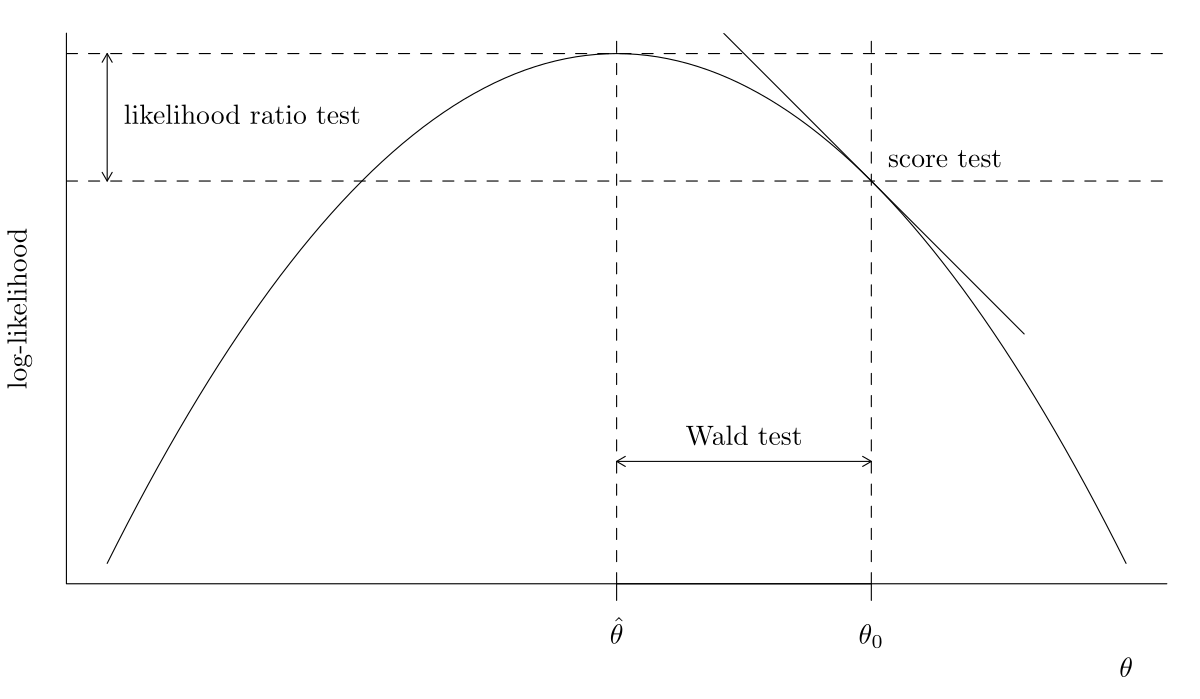
\includegraphics[width=0.85\textwidth,height=\textheight]{images/likelihood_tests.png}

}

\caption{Log-likelihood curve: the three likelihood-based tests, namely
Wald, likelihood ratio and score tests, are shown on the curve. The
tests use different information about the function.}

\end{figure}%

The three main classes of statistics for testing a simple null
hypothesis \(\mathscr{H}_0: \boldsymbol{\theta}=\boldsymbol{\theta}_0\)
against the alternative
\(\mathscr{H}_a: \boldsymbol{\theta} \neq \boldsymbol{\theta}_0\) are
the Wald, likelihood ratio, and the score test statistics, defined
respectively as \begin{align*}
 W &= (\widehat{\boldsymbol{\theta}}-\boldsymbol{\theta}_0)^\top j(\widehat{\boldsymbol{\theta}})(\widehat{\boldsymbol{\theta}}-\boldsymbol{\theta}_0),
 R &= 2 \left\{ \ell(\widehat{\boldsymbol{\theta}})-\ell(\boldsymbol{\theta}_0)\right\}, \\
 S &= U^\top(\boldsymbol{\theta}_0)i^{-1}(\boldsymbol{\theta}_0)U(\boldsymbol{\theta}_0), \\
\end{align*} where \(\widehat{\boldsymbol{\theta}}\) is the maximum
likelihood estimate under the alternative and \(\boldsymbol{\theta}_0\)
is the null value of the parameter vector. Asymptotically, all the test
statistics are equivalent (in the sense that they lead to the same
conclusions about \(\mathscr{H}_0\)). If \(\mathscr{H}_0\) is true, the
three test statistics follow asymptotically a \(\chi^2_q\) distribution
under a null hypothesis \(\mathscr{H}_0,\) where the degrees of freedom
\(q\) are the number of restrictions. \begin{align*}
w(\theta_0)&=(\widehat{\theta}-\theta_0)/\mathsf{se}(\widehat{\theta}) \\
r({\theta_0}) = \mathrm{sign}(\widehat{\theta}-\theta)\left[2
\left\{\ell(\widehat{\theta})-\ell(\theta)\right\}\right]^{1/2} \\
s(\theta_0)&=j^{-1/2}(\theta_0)U(\theta_0)
\end{align*} We call \(r({\theta_0})\) the directed likelihood root.

The likelihood ratio test statistic is normally the most powerful of the
three likelihood tests. The score statistic \(S\) only requires
calculation of the score and information under \(\mathscr{H}_0\)
(because by definition \(U(\widehat{\theta})=0\)), so it can be useful
in problems where calculations of the maximum likelihood estimator under
the alternative is costly or impossible.

\begin{figure}[ht!]

\centering{

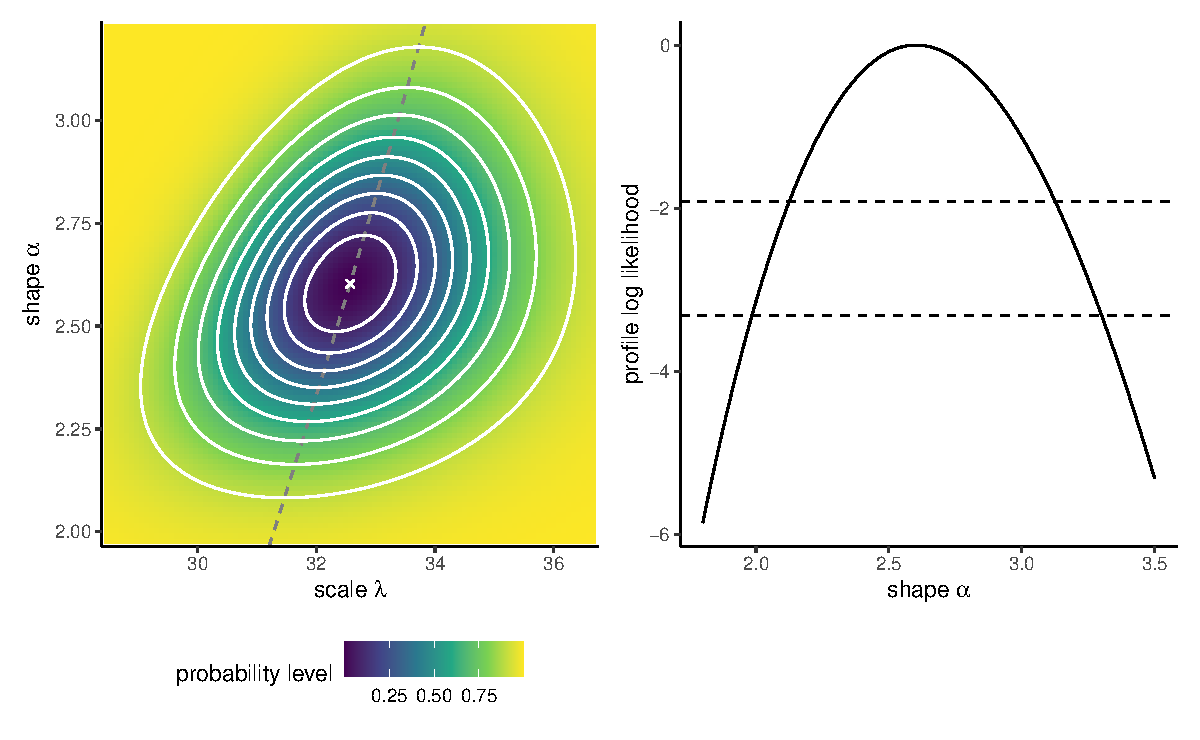
\includegraphics[width=0.85\textwidth,height=\textheight]{likelihood_files/figure-pdf/fig-weibull-profile-1.pdf}

}

\caption{\label{fig-weibull-profile}Profile log likelihood for
\(\alpha\), shown as a dashed gray line (left) and as a transect
(right). The left panel shows the log likelihood surface for the Weibull
model applied to the \texttt{waiting} data with 10\%, 20\%, \ldots, 90\%
likelihood ratio confidence regions (white contour curves). Higher log
likelihood values are indicated by darker colors. The cross indicates
the maximum likelihood estimate. The profile on the right hand panel has
been shifted vertically to be zero at the MLE; the dashed horizontal
lines denote the cutoff points for the 95\% and 99\% confidence
intervals.}

\end{figure}%

The Wald statistic \(W\) is the most widely encountered statistic and
two-sided 95\% confidence intervals for a single parameter \(\theta\)
are of the form \begin{align*}
\widehat{\theta} \pm \mathfrak{z}_{1-\alpha/2}\mathrm{se}(\widehat{\theta}),
\end{align*} where \(\mathfrak{z}_{1-\alpha/2}\) is the \(1-\alpha/2\)
quantile of the standard normal distribution; for a \(95\)\% confidence
interval, the \(0.975\) quantile of the normal distribution is
\(\mathfrak{z}_{0.975}=1.96.\) The Wald-based confidence intervals are
by construction \textbf{symmetric}: they may include implausible values
(e.g., negative values for if the parameter of interest \(\theta\) is
positive, such as variances).

\begin{example}[Wald test to compare exponential and Weibull
models]\protect\hypertarget{exm-weibull-exponential-submodel}{}\label{exm-weibull-exponential-submodel}

We can test whether the exponential model is an adequate simplification
of the Weibull distribution by imposing the restriction
\(\mathscr{H}_0: \alpha=1\). This imposes a single restriction to the
model, so we compare the square statistic to a \(\chi^2_1\). Since
\(\alpha\) is directly a parameter of the distribution, we have the
standard errors for free.

\begin{Shaded}
\begin{Highlighting}[]
\CommentTok{\# Calculate Wald statistic}
\NormalTok{wald\_exp }\OtherTok{\textless{}{-}}\NormalTok{ (mle\_weibull[}\DecValTok{2}\NormalTok{] }\SpecialCharTok{{-}} \DecValTok{1}\NormalTok{)}\SpecialCharTok{/}\NormalTok{se\_weibull[}\DecValTok{2}\NormalTok{]}
\CommentTok{\# Compute p{-}value}
\FunctionTok{pchisq}\NormalTok{(wald\_exp}\SpecialCharTok{\^{}}\DecValTok{2}\NormalTok{, }\AttributeTok{df =} \DecValTok{1}\NormalTok{, }\AttributeTok{lower.tail =} \ConstantTok{FALSE}\NormalTok{)}
\CommentTok{\#\textgreater{} [1] 3.61e{-}10}
\CommentTok{\# p{-}value less than 5\%, reject null}
\CommentTok{\# Obtain 95\% confidence intervals}
\NormalTok{mle\_weibull[}\DecValTok{2}\NormalTok{] }\SpecialCharTok{+} \FunctionTok{qnorm}\NormalTok{(}\FunctionTok{c}\NormalTok{(}\FloatTok{0.025}\NormalTok{, }\FloatTok{0.975}\NormalTok{))}\SpecialCharTok{*}\NormalTok{se\_weibull[}\DecValTok{2}\NormalTok{]}
\CommentTok{\#\textgreater{} [1] 2.1 3.1}
\CommentTok{\# 1 is not inside the confidence interval, reject null}
\end{Highlighting}
\end{Shaded}

We reject the null hypothesis, meaning the exponential submodel is not
an adequate simplification of the Weibull.

We can also check the goodness-of-fit of both models by drawing a
quantile-quantile plot (cf. Definition~\ref{def-qqplot}). It is apparent
from Figure~\ref{fig-qqplots-weibull-exp} that the exponential model is
overestimating the largest waiting times, whose dispersion in the sample
is less than that implied by the model. By contrast, the near perfect
straight line for the Weibull model in the right panel of
Figure~\ref{fig-qqplots-weibull-exp} suggests that the model fit is
adequate.

\begin{figure}[ht!]

\centering{

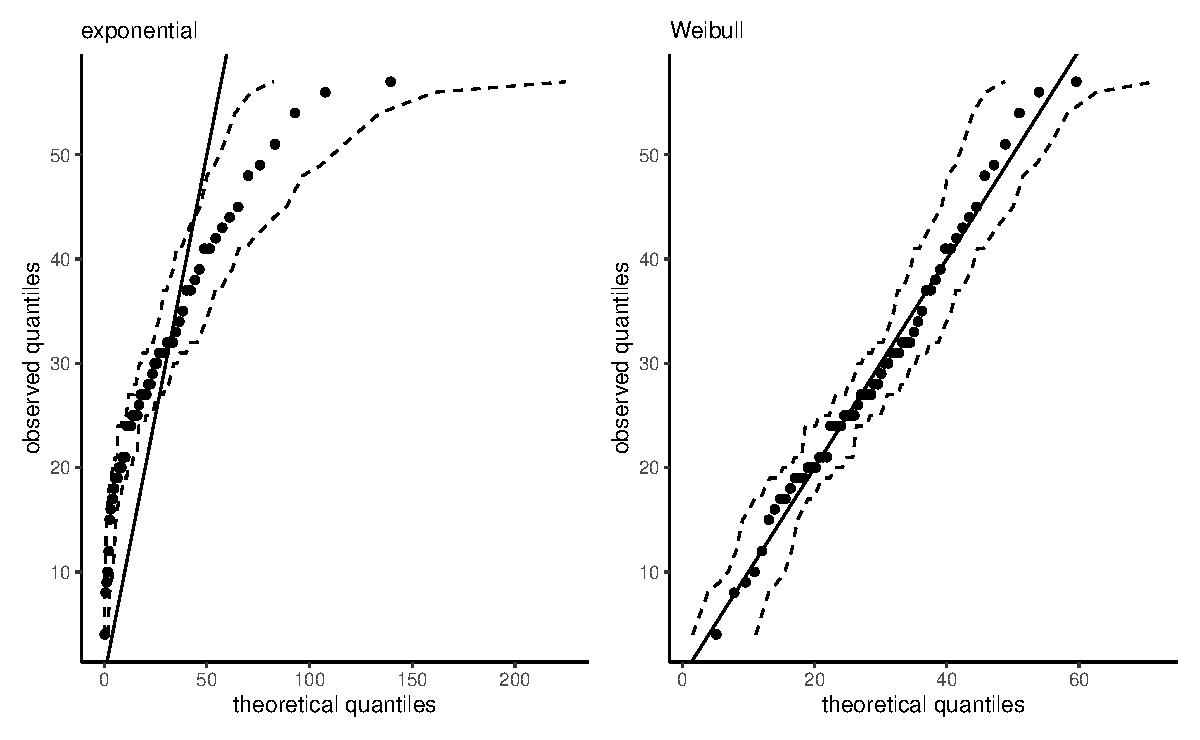
\includegraphics[width=0.85\textwidth,height=\textheight]{likelihood_files/figure-pdf/fig-qqplots-weibull-exp-1.pdf}

}

\caption{\label{fig-qqplots-weibull-exp}Quantile-quantile plots for
exponential (left) and Weibull (right) models, with 95\% pointwise
simulation intervals.}

\end{figure}%

\end{example}

\begin{refremark}[Lack of invariance of Wald-based confidence intervals]
The Wald-based confidence intervals are not parametrization invariant:
if we want intervals for a nonlinear continuous function \(g(\theta),\)
then in general
\(\mathsf{CI}_{W}\{g(\theta)\} \neq g\{\mathsf{CI}_{W}(\theta)\}.\)

For example, consider the exponential submodel. We can invert the Wald
test statistic to get a symmetric 95\% confidence interval for \(\phi,\)
\([0.061,\) \(0.191].\) If we were to naively transform the confidence
interval for \(\lambda\) into one for \(\phi,\) we would get \([0.063,\)
\(0.19],\) which highlights the invariance although the difference here
is subtle. The Gaussian approximation underlying the Wald test is
reliable if the sampling distribution of the likelihood is near
quadratic, which happens when the likelihood function is roughly
symmetric on either side of the maximum likelihood estimator.

\label{rem-invariance-wald-intervals}

\end{refremark}

The likelihood ratio test is invariant to interest-preserving
reparametrizations, so the test statistic for
\(\mathscr{H}_0: \phi=\phi_0\) and
\(\mathscr{H}_0: \lambda = -60/\ln(\phi_0)\) are the same. The Wald
confidence regions can be contrasted with the (better) ones derived
using the likelihood ratio test: these are found through a numerical
search to find the limits of \begin{align*}
\left\{\theta: 2\{\ell(\widehat{\boldsymbol{\theta}}) - \ell(\boldsymbol{\theta})\} \leq \chi^2_p(1-\alpha)\right\},
\end{align*} where \(\chi^2_p(1-\alpha)\) is the \((1-\alpha)\) quantile
of the \(\chi^2_p\) distribution. Such intervals, for
\(\alpha = 0.1, \ldots, 0.9\), appear in
Figure~\ref{fig-weibull-profile} as contour curves. If
\(\boldsymbol{\theta}\) is multidimensional, confidence intervals for
\(\theta_i\) are derived using the profile likelihood, discussed in the
sequel. Likelihood ratio-based confidence intervals are
\textbf{parametrization invariant}, so
\(\mathsf{CI}_{R}\{g(\theta)\} = g\{\mathsf{CI}_{R}(\theta)\}.\) Because
the likelihood is zero if a parameter value falls outside the range of
possible values for the parameter, the intervals only include plausible
values of \(\theta.\) In general, the intervals are asymmetric and have
better coverage properties.

\begin{Shaded}
\begin{Highlighting}[]
\CommentTok{\# Exponential log likelihood}
\NormalTok{ll\_exp }\OtherTok{\textless{}{-}} \ControlFlowTok{function}\NormalTok{(lambda)\{}
  \FunctionTok{sum}\NormalTok{(}\FunctionTok{dexp}\NormalTok{(waiting, }\AttributeTok{rate =} \DecValTok{1}\SpecialCharTok{/}\NormalTok{lambda, }\AttributeTok{log =} \ConstantTok{TRUE}\NormalTok{))}
\NormalTok{\}}
\CommentTok{\# MLE of the scale parameter}
\NormalTok{lambda\_hat }\OtherTok{\textless{}{-}} \FunctionTok{mean}\NormalTok{(waiting)}
\CommentTok{\# Root search for the limits of the confidence interval}
\NormalTok{lrt\_lb }\OtherTok{\textless{}{-}} \FunctionTok{uniroot}\NormalTok{( }\CommentTok{\# lower bound, using values below MLE}
  \AttributeTok{f =} \ControlFlowTok{function}\NormalTok{(r)\{}
     \DecValTok{2}\SpecialCharTok{*}\NormalTok{(}\FunctionTok{ll\_exp}\NormalTok{(lambda\_hat) }\SpecialCharTok{{-}} \FunctionTok{ll\_exp}\NormalTok{(r)) }\SpecialCharTok{{-}} \FunctionTok{qchisq}\NormalTok{(}\FloatTok{0.95}\NormalTok{, }\DecValTok{1}\NormalTok{)\}, }
  \AttributeTok{interval =} \FunctionTok{c}\NormalTok{(}\FloatTok{0.5} \SpecialCharTok{*} \FunctionTok{min}\NormalTok{(waiting), lambda\_hat))}\SpecialCharTok{$}\NormalTok{root}
\NormalTok{lrt\_ub }\OtherTok{\textless{}{-}} \FunctionTok{uniroot}\NormalTok{( }\CommentTok{\# upper bound,}
  \AttributeTok{f =} \ControlFlowTok{function}\NormalTok{(r)\{}
     \DecValTok{2}\SpecialCharTok{*}\NormalTok{(}\FunctionTok{ll\_exp}\NormalTok{(lambda\_hat) }\SpecialCharTok{{-}} \FunctionTok{ll\_exp}\NormalTok{(r)) }\SpecialCharTok{{-}} \FunctionTok{qchisq}\NormalTok{(}\FloatTok{0.95}\NormalTok{, }\DecValTok{1}\NormalTok{)\}, }
  \AttributeTok{interval =} \FunctionTok{c}\NormalTok{(lambda\_hat, }\DecValTok{2} \SpecialCharTok{*} \FunctionTok{max}\NormalTok{(waiting)))}\SpecialCharTok{$}\NormalTok{root}
\end{Highlighting}
\end{Shaded}

The likelihood ratio statistic 95\% confidence interval for \(\phi\) can
be found by using a root finding algorithm: the 95\% confidence interval
for \(\lambda\) is \(\mathsf{CI}_R(\lambda)[22.784,\) \(37.515].\) By
invariance, the 95\% confidence interval for \(\phi\) is
\(\mathsf{CI}_R(\phi) = [0.072, 0.202] = g
\{\mathsf{CI}_R(\lambda)\}.\)

\section{Profile likelihood}\label{profile-likelihood}

Sometimes, we may want to perform hypothesis test or derive confidence
intervals for selected components of the model. In this case, the null
hypothesis only restricts part of the space and the other parameters,
termed nuisance, are left unspecified --- the question then is what
values to use for comparison with the full model. It turns out that the
values that maximize the constrained log likelihood are what one should
use for the test, and the particular function in which these nuisance
parameters are integrated out is termed a profile likelihood.

\begin{definition}[Profile log
likelihood]\protect\hypertarget{def-profile}{}\label{def-profile}

Consider a parametric model with log likelihood function
\(\ell(\boldsymbol{\theta})\) whose \(p\)-dimensional parameter vector
\(\boldsymbol{\theta}=(\boldsymbol{\psi}, \boldsymbol{\varphi})\) can be
decomposed into a \(q\)-dimensional parameter of interest
\(\boldsymbol{\psi}\) and a \((p-q)\)-dimensional nuisance vector
\(\boldsymbol{\varphi}.\)

The profile likelihood \(\ell_{\mathsf{p}},\) a function of
\(\boldsymbol{\psi}\) alone, is obtained by maximizing the likelihood
pointwise at each fixed value \(\boldsymbol{\psi}_0\) over the nuisance
vector \(\boldsymbol{\varphi}_{\psi_0},\) \begin{align*}
\ell_{\mathsf{p}}(\boldsymbol{\psi})=\max_{\boldsymbol{\varphi}}\ell(\boldsymbol{\psi}, \boldsymbol{\varphi})=\ell(\boldsymbol{\psi}, \widehat{\boldsymbol{\varphi}}_{\boldsymbol{\psi}}).
\end{align*}

\end{definition}

\begin{example}[Profile log likelihood for the Weibull shape
parameter]\protect\hypertarget{exm-profile-alpha-weibull}{}\label{exm-profile-alpha-weibull}

Consider the shape parameter \(\psi \equiv\alpha\) as parameter of
interest, and the scale \(\varphi\equiv\lambda\) as nuisance parameter.
Using the gradients derived in Example~\ref{exm-weibull-mle}, we find
that the value of the scale that maximizes the log likelihood for given
\(\alpha\) is \begin{align*}
\widehat{\lambda}_\alpha = \left( \frac{1}{n}\sum_{i=1}^n y_i^\alpha\right)^{1/\alpha}.
\end{align*} and plugging in this value gives a function of \(\alpha\)
alone, thereby also reducing the optimization problem for the Weibull to
a line search along \(\ell_{\mathsf{p}}(\alpha)\). The left hand panel
of Figure~\ref{fig-weibull-profile} shows the ridge along the direction
of \(\alpha\) corresponding to the log likelihood surface. If one thinks
of these contours lines as those of a topographic map, the profile
likelihood corresponds in this case to walking along the ridge of both
mountains along the \(\psi\) direction, with the right panel showing the
elevation gain/loss. The corresponding elevation profile on the right of
Figure~\ref{fig-weibull-profile} with cutoff values. We would need to
obtain numerically using a root finding algorithm the limits of the
confidence interval on either side of \(\widehat{\alpha}\), but it's
clear that \(\alpha=1\) is not inside the 99\% interval.

\begin{Shaded}
\begin{Highlighting}[]
\NormalTok{lambda\_alpha }\OtherTok{\textless{}{-}} \ControlFlowTok{function}\NormalTok{(alpha, }\AttributeTok{y =}\NormalTok{ waiting)\{}
\NormalTok{  (}\FunctionTok{mean}\NormalTok{(y}\SpecialCharTok{\^{}}\NormalTok{alpha))}\SpecialCharTok{\^{}}\NormalTok{(}\DecValTok{1}\SpecialCharTok{/}\NormalTok{alpha)}
\NormalTok{\}}
\CommentTok{\# Profile likelihood for alpha}
\NormalTok{prof\_alpha\_weibull }\OtherTok{\textless{}{-}} \ControlFlowTok{function}\NormalTok{(par, }\AttributeTok{y =}\NormalTok{ waiting)\{}
  \FunctionTok{sapply}\NormalTok{(par, }\ControlFlowTok{function}\NormalTok{(a)\{}
   \FunctionTok{nll\_weibull}\NormalTok{(}\AttributeTok{pars =} \FunctionTok{c}\NormalTok{(}\FunctionTok{lambda\_alpha}\NormalTok{(a), a), }\AttributeTok{y =}\NormalTok{ y)}
\NormalTok{  \})}
\NormalTok{\}}
\end{Highlighting}
\end{Shaded}

\end{example}

\begin{example}[Profile log likelihood for the Weibull
mean]\protect\hypertarget{exm-profile-mean-weibull}{}\label{exm-profile-mean-weibull}

As an alternative, we can use numerical optimization to compute the
profile for another function. Suppose we are interested in the expected
waiting time, which according to the model is
\(\mu = \mathsf{E}(Y) = \lambda\Gamma(1+1/\alpha)\). To this effect, we
reparametrize the model in terms of \((\mu, \alpha)\), where
\(\lambda=\mu/\Gamma(1+1/\alpha)\). We then make a wrapper function that
optimizes the log likelihood for fixed value of \(\mu\), then returns
\(\widehat{\alpha}_{\mu}\), \(\mu\) and \(\ell_{\mathrm{p}}(\mu)\).

To get the confidence intervals for a scalar parameter, there is a trick
that helps with the derivation. We compute the signed likelihood root
\(r(\psi) = \mathrm{sign}(\psi - \widehat{\psi})\{2\ell_{\mathrm{p}}(\widehat{\psi}) -2 \ell_{\mathrm{p}}(\psi)\}^{1/2}\)
over a fine grid of \(\psi\), then fit a smoothing spline to the
equation flipping the axis (thus, the model has response \(y=\psi\) and
\(x=r(\psi)\)). We then predict the curve at the standard normal
quantiles \(\mathfrak{z}_{\alpha/2}\) and \(\mathfrak{z}_{1-\alpha/2}\),
and return these values as confidence interval.
Figure~\ref{fig-profile-mu-weibull} shows how these value correspond to
the cutoff points on the log likelihood ratio scale, where the vertical
line is given by \(-\mathfrak{c}(1-\alpha)/2\) where \(\mathfrak{c}\)
denotes the quantile of a \(\chi^2_1\) random variable.

\begin{Shaded}
\begin{Highlighting}[]
\CommentTok{\# Compute the MLE for the expected value via plug{-}in}
\NormalTok{mu\_hat }\OtherTok{\textless{}{-}}\NormalTok{ mle\_weibull[}\DecValTok{1}\NormalTok{]}\SpecialCharTok{*}\FunctionTok{gamma}\NormalTok{(}\DecValTok{1}\SpecialCharTok{+}\DecValTok{1}\SpecialCharTok{/}\NormalTok{mle\_weibull[}\DecValTok{2}\NormalTok{])}
\CommentTok{\# Create a profile function}
\NormalTok{prof\_weibull\_mu }\OtherTok{\textless{}{-}} \ControlFlowTok{function}\NormalTok{(mu)\{}
  \CommentTok{\# For given value of mu}
\NormalTok{  alpha\_mu }\OtherTok{\textless{}{-}} \ControlFlowTok{function}\NormalTok{(mu)\{ }
  \CommentTok{\# Find the profile by optimizing (line search) for fixed mu and the best alpha}
\NormalTok{     opt }\OtherTok{\textless{}{-}} \FunctionTok{optimize}\NormalTok{(}\AttributeTok{f =} \ControlFlowTok{function}\NormalTok{(alpha, mu)\{}
     \CommentTok{\# minimize the negative log likelihood}
      \FunctionTok{nll\_weibull}\NormalTok{(}\FunctionTok{c}\NormalTok{(mu}\SpecialCharTok{/}\FunctionTok{gamma}\NormalTok{(}\DecValTok{1}\SpecialCharTok{+}\DecValTok{1}\SpecialCharTok{/}\NormalTok{alpha), alpha), }\AttributeTok{y =}\NormalTok{ waiting)\}, }
   \AttributeTok{mu =}\NormalTok{ mu, }
  \AttributeTok{interval =} \FunctionTok{c}\NormalTok{(}\FloatTok{0.1}\NormalTok{,}\DecValTok{10}\NormalTok{) }\CommentTok{\#search region}
\NormalTok{  )}
  \CommentTok{\# Return the value of the negative log likelihood and alpha\_mu}
  \FunctionTok{return}\NormalTok{(}\FunctionTok{c}\NormalTok{(}\AttributeTok{nll =}\NormalTok{ opt}\SpecialCharTok{$}\NormalTok{objective, }\AttributeTok{alpha =}\NormalTok{ opt}\SpecialCharTok{$}\NormalTok{minimum))}
\NormalTok{  \}}
  \CommentTok{\# Create a data frame with mu and the other parameters}
  \FunctionTok{data.frame}\NormalTok{(}\AttributeTok{mu =}\NormalTok{ mu, }\FunctionTok{t}\NormalTok{(}\FunctionTok{sapply}\NormalTok{(mu, }\ControlFlowTok{function}\NormalTok{(m)\{}\FunctionTok{alpha\_mu}\NormalTok{(m)\})))}
\NormalTok{\}}
\CommentTok{\# Create a data frame with the profile  }
\NormalTok{prof }\OtherTok{\textless{}{-}} \FunctionTok{prof\_weibull\_mu}\NormalTok{(}\FunctionTok{seq}\NormalTok{(}\DecValTok{22}\NormalTok{, }\DecValTok{35}\NormalTok{, }\AttributeTok{length.out =} \DecValTok{101}\NormalTok{L))}
\CommentTok{\# Compute signed likelihood root r}
\NormalTok{prof}\SpecialCharTok{$}\NormalTok{r }\OtherTok{\textless{}{-}} \FunctionTok{sign}\NormalTok{(prof}\SpecialCharTok{$}\NormalTok{mu }\SpecialCharTok{{-}}\NormalTok{ mu\_hat)}\SpecialCharTok{*}\FunctionTok{sqrt}\NormalTok{(}\DecValTok{2}\SpecialCharTok{*}\NormalTok{(prof}\SpecialCharTok{$}\NormalTok{nll }\SpecialCharTok{{-}}\NormalTok{ opt\_weibull}\SpecialCharTok{$}\NormalTok{value))}

\CommentTok{\# Trick: fit a spline to obtain the predictions with mu as a function of r}
\CommentTok{\# Then use this to predict the value at which we intersect the normal quantiles}
\NormalTok{fit.r }\OtherTok{\textless{}{-}}\NormalTok{ stats}\SpecialCharTok{::}\FunctionTok{smooth.spline}\NormalTok{(}\AttributeTok{x =} \FunctionTok{cbind}\NormalTok{(prof}\SpecialCharTok{$}\NormalTok{r, prof}\SpecialCharTok{$}\NormalTok{mu), }\AttributeTok{cv =} \ConstantTok{FALSE}\NormalTok{)}
\NormalTok{pr }\OtherTok{\textless{}{-}} \FunctionTok{predict}\NormalTok{(fit.r, }\FunctionTok{qnorm}\NormalTok{(}\FunctionTok{c}\NormalTok{(}\FloatTok{0.025}\NormalTok{, }\FloatTok{0.975}\NormalTok{)))}\SpecialCharTok{$}\NormalTok{y}
\CommentTok{\# Plot the signed likelihood root {-} near linear indicates quadratic}
\NormalTok{g1 }\OtherTok{\textless{}{-}} \FunctionTok{ggplot}\NormalTok{(}\AttributeTok{data =}\NormalTok{ prof,}
     \AttributeTok{mapping =} \FunctionTok{aes}\NormalTok{(}\AttributeTok{x =}\NormalTok{ mu, }\AttributeTok{y =}\NormalTok{ r)) }\SpecialCharTok{+}
  \FunctionTok{geom\_abline}\NormalTok{(}\AttributeTok{intercept =} \DecValTok{0}\NormalTok{, }\AttributeTok{slope =} \DecValTok{1}\NormalTok{) }\SpecialCharTok{+}
  \FunctionTok{geom\_line}\NormalTok{() }\SpecialCharTok{+} 
  \FunctionTok{geom\_hline}\NormalTok{(}\AttributeTok{yintercept =} \FunctionTok{qnorm}\NormalTok{(}\FloatTok{0.025}\NormalTok{, }\FloatTok{0.975}\NormalTok{),}
            \AttributeTok{linetype =} \StringTok{"dashed"}\NormalTok{) }\SpecialCharTok{+} 
  \FunctionTok{labs}\NormalTok{(}\AttributeTok{x =} \FunctionTok{expression}\NormalTok{(}\FunctionTok{paste}\NormalTok{(}\StringTok{"expectation "}\NormalTok{, mu)),}
       \AttributeTok{y =} \StringTok{"signed likelihood root"}\NormalTok{)}
\CommentTok{\# Create a plot of the profile}
\NormalTok{g2 }\OtherTok{\textless{}{-}} \FunctionTok{ggplot}\NormalTok{(}\AttributeTok{data =}\NormalTok{ prof,}
       \AttributeTok{mapping =} \FunctionTok{aes}\NormalTok{(}\AttributeTok{x =}\NormalTok{ mu, }\AttributeTok{y =}\NormalTok{ opt\_weibull}\SpecialCharTok{$}\NormalTok{value }\SpecialCharTok{{-}}\NormalTok{ nll)) }\SpecialCharTok{+} 
  \FunctionTok{geom\_line}\NormalTok{() }\SpecialCharTok{+}
  \FunctionTok{geom\_hline}\NormalTok{(}\AttributeTok{yintercept =} \SpecialCharTok{{-}}\FunctionTok{qchisq}\NormalTok{(}\FunctionTok{c}\NormalTok{(}\FloatTok{0.95}\NormalTok{), }\AttributeTok{df =} \DecValTok{1}\NormalTok{)}\SpecialCharTok{/}\DecValTok{2}\NormalTok{,}
             \AttributeTok{linetype =} \StringTok{"dashed"}\NormalTok{) }\SpecialCharTok{+}
  \FunctionTok{geom\_vline}\NormalTok{(}\AttributeTok{linetype =} \StringTok{"dotted"}\NormalTok{,}
  \AttributeTok{xintercept =}\NormalTok{ pr) }\SpecialCharTok{+} 
  \FunctionTok{labs}\NormalTok{(}\AttributeTok{x =} \FunctionTok{expression}\NormalTok{(}\FunctionTok{paste}\NormalTok{(}\StringTok{"expectation "}\NormalTok{, mu)),}
       \AttributeTok{y =} \StringTok{"profile log likelihood"}\NormalTok{)}

\NormalTok{g1 }\SpecialCharTok{+}\NormalTok{ g2}
\end{Highlighting}
\end{Shaded}

\begin{figure}[ht!]

\centering{

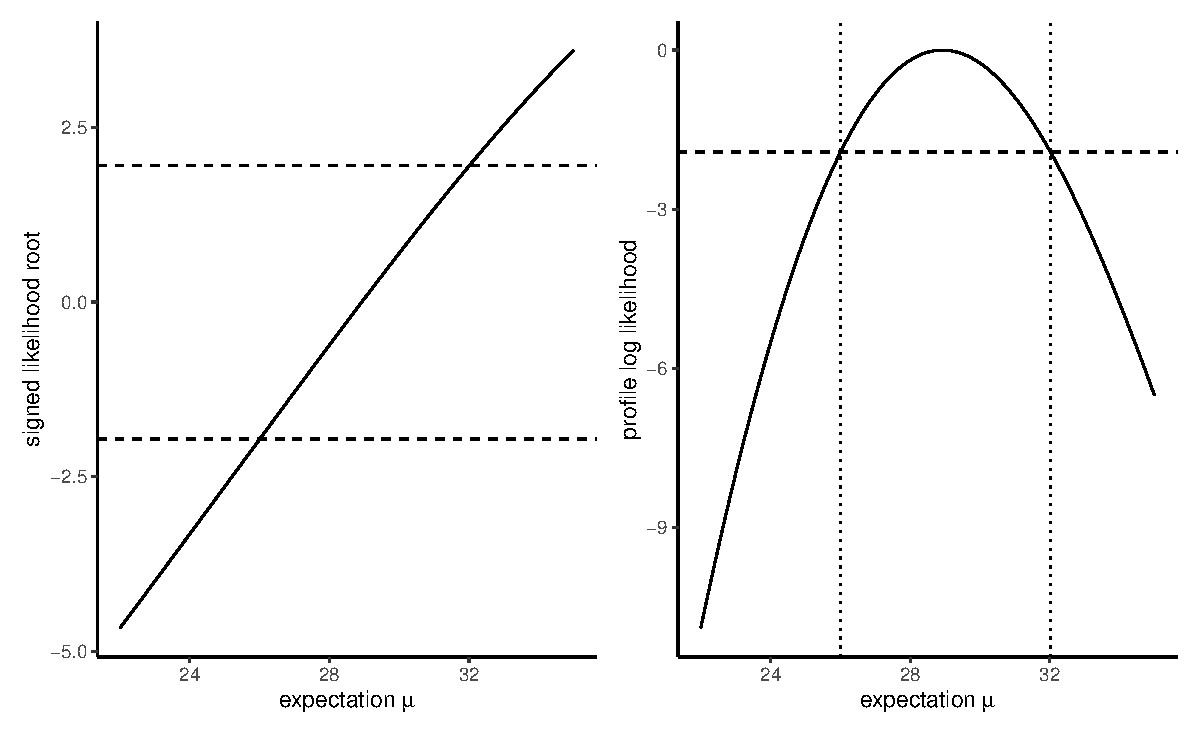
\includegraphics[width=0.85\textwidth,height=\textheight]{likelihood_files/figure-pdf/fig-profile-mu-weibull-1.pdf}

}

\caption{\label{fig-profile-mu-weibull}Signed likelihood root (left) and
shifted profile log likelihood (right) as a function of the expected
value \(\mu\) in the Weibull model.}

\end{figure}%

\end{example}

The maximum profile likelihood estimator behaves like a regular
likelihood for most quantities of interest and we can derive test
statistics and confidence intervals in the usual way. One famous example
of profile likelihood is the Cox proportional hazard covered in
\hyperref[survival]{Chapter 7}.

\section{Information criteria}\label{information-criteria}

The likelihood can also serve as building block for model comparison:
the larger \(\ell(\boldsymbol{\widehat{\theta}})\), the better the fit.
However, the likelihood doesn't account for model complexity in the
sense that more complex models with more parameters lead to higher
likelihood. This is not a problem for comparison of nested models using
the likelihood ratio test because we look only at relative improvement
in fit. There is a danger of \textbf{overfitting} if we only consider
the likelihood of a model.

\(\mathsf{AIC}\) and \(\mathsf{BIC}\) are information criteria measuring
how well the model fits the data, while penalizing models with more
parameters, \begin{align*}
\mathsf{AIC}&=-2\ell(\widehat{\boldsymbol{\theta}})+2p \\
\mathsf{BIC}&=-2\ell(\widehat{\boldsymbol{\theta}})+p\ln(n),
\end{align*} where \(p\) is the number of parameters in the model. The
smaller the value of \(\mathsf{AIC}\) (or of \(\mathsf{BIC}\)), the
better the model fit.

Note that information criteria do not constitute formal hypothesis tests
on the parameters, but they can be used to compare models that are not
nested. Such tools work under regularity conditions, and the estimated
information criteria are quite noisy, so comparison for non-nested
models are hazardous although popular among practitioners. If we want to
compare likelihood from different probability models, we need to make
sure they include normalizing constant. The \(\mathsf{BIC}\) is more
stringent than \(\mathsf{AIC}\), as its penalty increases with the
sample size, so it selects models with fewer parameters. The
\(\mathsf{BIC}\) is \textbf{consistent}, meaning that it will pick the
true correct model from an ensemble of models with probability one as
\(n \to \infty\). In practice, this is of little interest if one assumes
that all models are approximation of reality (it is unlikely that the
true model is included in the ones we consider). \(\mathsf{AIC}\) often
selects overly complicated models in large samples, whereas
\(\mathsf{BIC}\) chooses models that are overly simple.

A cautionary warning: while you can compare regression models that are
not nested using information criteria, they can only be used when the
response variable is the same. You could compare a Poisson regression
with a linear regression for some response \(Y\) using information
criteria provided you include all normalizing constants in your model.
Software often drops constant terms; this has no impact when you compare
models with the same constant factors, but it matters when these differ.
However, \textbf{you cannot} compare them to a log-linear model with
response \(\ln(Y)\). Comparisons for log-linear and linear models are
valid only if you use the Box--Cox likelihood, as it includes the
Jacobian of the transformation.

\bookmarksetup{startatroot}

\chapter{Linear regression models}\label{linmod}

\section{Introduction}\label{introduction}

The linear regression model, or linear model, is one of the most
versatile workhorse for statistical inference. Linear regression is used
primarily to evaluate the effects of explanatory variables (oftentimes
treatment in an experimental setting) on the mean response of a
continuous response, or for prediction. It combines a formulation for
the mean of a \textbf{response variable} \(Y_i\) of a random sample of
size \(n\) as a \textbf{linear function} of observed
\textbf{explanatories} (also called predictors or covariates)
\(X_1, \ldots, X_p\), \begin{align}
\underset{\text{conditional mean}}{\mathsf{E}(Y_i \mid \boldsymbol{X}_i=\boldsymbol{x}_i)}=\mu_i=\underset{\text{linear combination of explanatories}}{\beta_0 + \beta_1x_{i1} + \cdots + \beta_p x_{ip}}\equiv \mathbf{x}_i\boldsymbol{\beta}.
\end{align} where \(\mathbf{x}_i = (1, x_{i1}, \ldots, x_{ip})\) is a
\((p+1)\) row vector containing a constant and the explanatories of
observation \(i\), and
\(\boldsymbol{\beta} = (\beta_0, \ldots, \beta_p)^\top\) is a \(p+1\)
column vector of coefficients for the mean. The model formulation is
conditional on the values of the observed explanatories; this amounts to
treating the \(p\) explanatory variables \(X_1, \ldots, X_p\) as
non-random quantities, or known in advance. The regression coefficients
\(\boldsymbol{\beta}\) is the same for all observations, but the vector
of explanatories \(\mathbf{x}_i\) may change from one observation to the
next. The model is \textbf{linear} in the coefficients
\(\beta_0, \ldots, \beta_p\).

For notational simplicity, we aggregate observations into an
\(n\)-vector \(\boldsymbol{Y}\) and the explanatories into an
\(n \times (p+1)\) matrix \(\mathbf{X}\) by concatenating a column of
ones and the \(p\) column vectors
\(\boldsymbol{X}_1, \ldots, \boldsymbol{X}_p\), each containing the
\(n\) observations of the respective explanatories. The matrix
\(\mathbf{X}\) is termed \textbf{model matrix} (or sometimes design
matrix in experimental settings), and it's \(i\)th row is
\(\mathbf{x}_i\).

We suppose, in addition to the mean specification, that the response
variables are independent and identically distributed, drawn from a
mean-zero distribution with constant variance \(\sigma^2\). Assuming
that the distribution are drawn from a location family, we may rewrite
the linear model in terms of the mean plus an error term, \begin{align*}
\underset{\text{observation}\vphantom{\mu_i}}{Y_i} = \underset{\text{mean } \mu_i}{\vphantom{Y_i}\mathbf{x}_i\boldsymbol{\beta}} + \underset{\text{error term}\vphantom{\mu_i}}{\vphantom{Y_i}\varepsilon_i}.
\end{align*} where \(\varepsilon_i\) is the error term specific to
observation \(i\), and we assume that the errors
\(\varepsilon_1, \ldots, \varepsilon_n\) are independent and identically
distributed. We fix the expectation or theoretical mean of
\(\varepsilon_i\) to zero to encode the fact we do not believe the model
is systematically off, so
\(\mathsf{E}(\varepsilon_i \mid \boldsymbol{X}_i=\boldsymbol{x}_i)=0\)
\((i=1, \ldots, n)\). The variance term \(\sigma^2\) is included to take
into account the fact that no exact linear relationship links
\(\boldsymbol{X}_i\) and \(Y_i\), or that measurements of \(Y_i\) are
subject to error.

The normal or Gaussian linear model specifies that responses follow a
normal distribution, with
\(Y_i \mid \boldsymbol{X}_i=\boldsymbol{x}_i \sim \mathsf{normal}(\mathbf{x}_i\boldsymbol{\beta}, \sigma^2)\).
The normal distribution is a location-scale family, so
\(Y \sim \mathsf{normal}(\mu, \sigma^2)\) is equal in distribution with
\(\mu + \varepsilon\) for
\(\varepsilon \sim \mathsf{normal}(0, \sigma^2)\).

\subsection{Motivating examples}\label{motivating-examples}

We present some motivating examples that are discussed in the sequel.

\begin{example}[Consistency of product
description]\protect\hypertarget{exm-lee-choi1}{}\label{exm-lee-choi1}

Study 1 of Lee and Choi (\citeproc{ref-Lee.Choi:2019}{2019}) considered
descriptors and the impact on the perception of a product on the
discrepancy between the text description and the image. In their first
experience, a set of six toothbrushes is sold, but the image shows
either a pack of six, or a single one). The authors also measured the
prior familiarity with the brand of the item. Participants were
recruited using an online panel, and the data in \texttt{LC19\_S1}
includes the results of the \(n=96\) participants who passed the
attention check (one additional participant response was outlying and
removed). We could fit a linear model for the average product evaluation
score, \texttt{prodeval}, as a function of the familiarity of the brand
\texttt{familiarity}, an integer ranging from 1 to 7, and a dummy
variable for the experimental factor \texttt{consistency}, coded
\texttt{0} for consistent image/text descriptions and \texttt{1} if
inconsistent. The resulting model matrix is then \(96 \times 3\). The
\texttt{prodeval} response is heavily discretized, with only 19 unique
values ranging between 2.33 and 9.

\begin{Shaded}
\begin{Highlighting}[]
\FunctionTok{data}\NormalTok{(LC19\_S1, }\AttributeTok{package =} \StringTok{"hecedsm"}\NormalTok{)}
\CommentTok{\# Fit a linear model using "lm"}
\CommentTok{\# The first argument is a formula of the form y \textasciitilde{} x1 + x2}
\CommentTok{\# where y is the response and x\textquotesingle{}s are explanatories, }
\CommentTok{\# separated by a plus (+) sign}
\NormalTok{mod }\OtherTok{\textless{}{-}} \FunctionTok{lm}\NormalTok{(prodeval }\SpecialCharTok{\textasciitilde{}}\NormalTok{ familiarity }\SpecialCharTok{+}\NormalTok{ consistency,}
          \AttributeTok{data =}\NormalTok{ LC19\_S1)}
\CommentTok{\# Extract the model matrix}
\FunctionTok{tail}\NormalTok{(}\FunctionTok{model.matrix}\NormalTok{(mod), }\AttributeTok{n =} \DecValTok{5}\NormalTok{L) }\CommentTok{\# first five lines}
\CommentTok{\#\textgreater{}    (Intercept) familiarity consistencyinconsistent}
\CommentTok{\#\textgreater{} 92           1           6                       1}
\CommentTok{\#\textgreater{} 93           1           4                       1}
\CommentTok{\#\textgreater{} 94           1           7                       1}
\CommentTok{\#\textgreater{} 95           1           7                       1}
\CommentTok{\#\textgreater{} 96           1           7                       1}
\FunctionTok{dim}\NormalTok{(}\FunctionTok{model.matrix}\NormalTok{(mod)) }\CommentTok{\# dimension of the model matrix}
\CommentTok{\#\textgreater{} [1] 96  3}
\end{Highlighting}
\end{Shaded}

\end{example}

\begin{example}[Gender discrimination in a US
college]\protect\hypertarget{exm-college-salary-discrimination}{}\label{exm-college-salary-discrimination}

To make concepts and theoretical notions more concrete, we will use
observational data collected in a college in the United States. The goal
of the administration was to investigate potential gender inequality in
the salary of faculty members. The data contains the following
variables:

\begin{itemize}
\tightlist
\item
  \texttt{salary}: nine-month salary of professors during the 2008--2009
  academic year (in thousands USD).
\item
  \texttt{rank}: academic rank of the professor (\texttt{assistant},
  \texttt{associate} or \texttt{full}).
\item
  \texttt{field}: categorical variable for the field of expertise of the
  professor, one of \texttt{applied} or \texttt{theoretical}.
\item
  \texttt{sex}: binary indicator for sex, either \texttt{man} or
  \texttt{woman}.
\item
  \texttt{service}: number of years of service in the college.
\item
  \texttt{years}: number of years since PhD.
\end{itemize}

Before drafting a model, it is useful to perform an exploratory data
analysis. If salary increases with year, there is more heterogeneity in
the salary of higher ranked professors: logically, assistant professors
are either promoted or kicked out after at most 6 years according to the
data. The limited number of years prevents large variability for their
salaries.

\begin{figure}[ht!]

{\centering 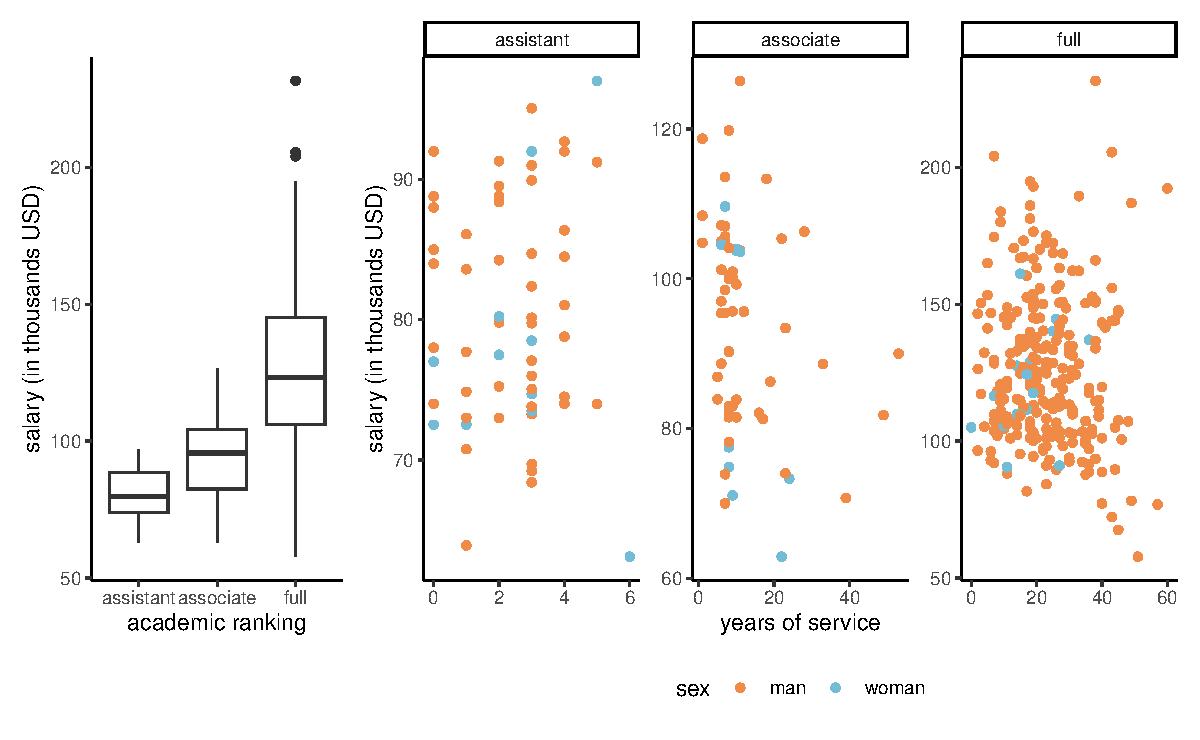
\includegraphics[width=0.85\textwidth,height=\textheight]{linearmodels_files/figure-pdf/edacollege-1.pdf}

}

\caption{Exploratory data analysis of \(\texttt{college}\) data:
salaries of professors as a function of the number of years of service
and the academic ranking}

\end{figure}%

Salary increases over years of service, but its variability also
increases with rank. Note the much smaller number of women in the
sample: this will impact our power to detect differences between sex. A
contingency table of sex and academic rank can be useful to see if the
proportion of women is the same in each rank: women represent 16\% of
assistant professors and 16\% of associate profs, but only 7\% of full
professors and these are better paid on average.

\begin{longtable}[]{@{}lrrr@{}}
\caption{Contingency table of the number of prof in the college by sex
and academic rank.}\tabularnewline
\toprule\noalign{}
& assistant & associate & full \\
\midrule\noalign{}
\endfirsthead
\toprule\noalign{}
& assistant & associate & full \\
\midrule\noalign{}
\endhead
\bottomrule\noalign{}
\endlastfoot
man & 56 & 54 & 248 \\
woman & 11 & 10 & 18 \\
\end{longtable}

Some of the potential explanatory variables of the \texttt{college} data
are categorical (\texttt{rank}, \texttt{sex}, \texttt{field}), the
latter two being binary. The other three variables, \texttt{years} and
\texttt{service}, are continuous and probably strongly correlated.

\end{example}

\begin{example}[Teaching to read and pre-post
experiments]\protect\hypertarget{exm-teaching-baumann}{}\label{exm-teaching-baumann}

The \texttt{BSJ92} data in package \texttt{hecedsm} contains the results
of an experimental study by Baumann, Seifert-Kessell, and Jones
(\citeproc{ref-Baumann:1992}{1992}) on the effectiveness of different
reading strategies on understanding of children. These are described in
the abstract

\begin{quote}
Sixty-six fourth-grade students were randomly assigned to one of three
experimental groups: (a) a Think-Aloud (TA) group, in which students
were taught various comprehension monitoring strategies for reading
stories (e.g., self-questioning, prediction, retelling, rereading)
through the medium of thinking aloud; (b) a Directed Reading-Thinking
Activity (DRTA) group, in which students were taught a predict-verify
strategy for reading and responding to stories; or (c) a Directed
Reading Activity (DRA) group, an instructed control, in which students
engaged in a noninteractive, guided reading of stories.
\end{quote}

The data are balanced, as there are 22 observations in each of the three
subgroups, of which \texttt{DR} is the control. The researchers applied
a series of three tests (an error detection task for test 1, a
comprehension monitoring questionnaire for test 2, and the \emph{Degrees
of Reading Power} cloze test labelled test 3). Tests 1 and 2 were
administered both before and after the intervention: this gives us a
change to establish the average \emph{improvement} in student by adding
\texttt{pretest1} as covariate for a regression of \texttt{posttest},
for example. The tests 1 were out of 16, but the one administered after
the experiment was made more difficult to avoid cases of students
getting near full scores. The correlation between pre-test and post-test
1 is \((\widehat{\rho}_1=0.57)\), much stronger than that for the second
test \((\widehat{\rho}_2=0.21)\).

\end{example}

\section{Mean model specification}\label{mean-model-specification}

This section covers the mean model specification, starting with
parametrization of models with factors (i.e., categorical
explanatories).

\subsection{What explanatories?}\label{what-explanatories}

The first step of an analysis is deciding which explanatory variables
should be added to the mean model specification, and under what form.
Models are but approximations of reality; Section 2.1 of Venables
(\citeproc{ref-Venables:2000}{2000}) argues that, if we believe the true
mean function linking explanatories \(\boldsymbol{X}\) and the response
\(Y\) is of the form
\(\mathsf{E}(Y \mid \boldsymbol{X}) = f(\boldsymbol{X})\) for \(f\)
sufficiently smooth, then the linear model is a first-order
approximation. For interpretation purposes, it makes sense to
mean-center any continuous explanatory, as this facilitates
interpretation.

In an experimental setting, where the experimental group or condition is
randomly allocated, we can directly compare the different treatments and
draw causal conclusions (since all other things are constant, any
detectable difference is due on average to our manipulation). Although
we usually refrain from including any other explanatory to keep the
design simple, it may be nevertheless helpful to consider some
concomitant variables that explain part of the variability to filter
background noise and increase power. For example, for the Baumann,
Seifert-Kessell, and Jones (\citeproc{ref-Baumann:1992}{1992}) data, our
interest is in comparing the average scores as a function of the
teaching method, we would include \texttt{group}. In this example, it
would also make sense to include the \texttt{pretest1} result as an
explanatory. This way, we will model the average difference in
improvement from pre-test to post-test rather than the average score.

In an observational setting, people self-select in different groups, so
we need to account for differences. Linear models in economics and
finance often add control variables to the model to account for
potential differences due to socio-demographic variables (age, revenue,
etc.) that would be correlated to the group. Any test for coefficients
would capture only correlation between the outcome \(Y\) and the
postulated explanatory factor of interest.

\begin{figure}[ht!]

{\centering 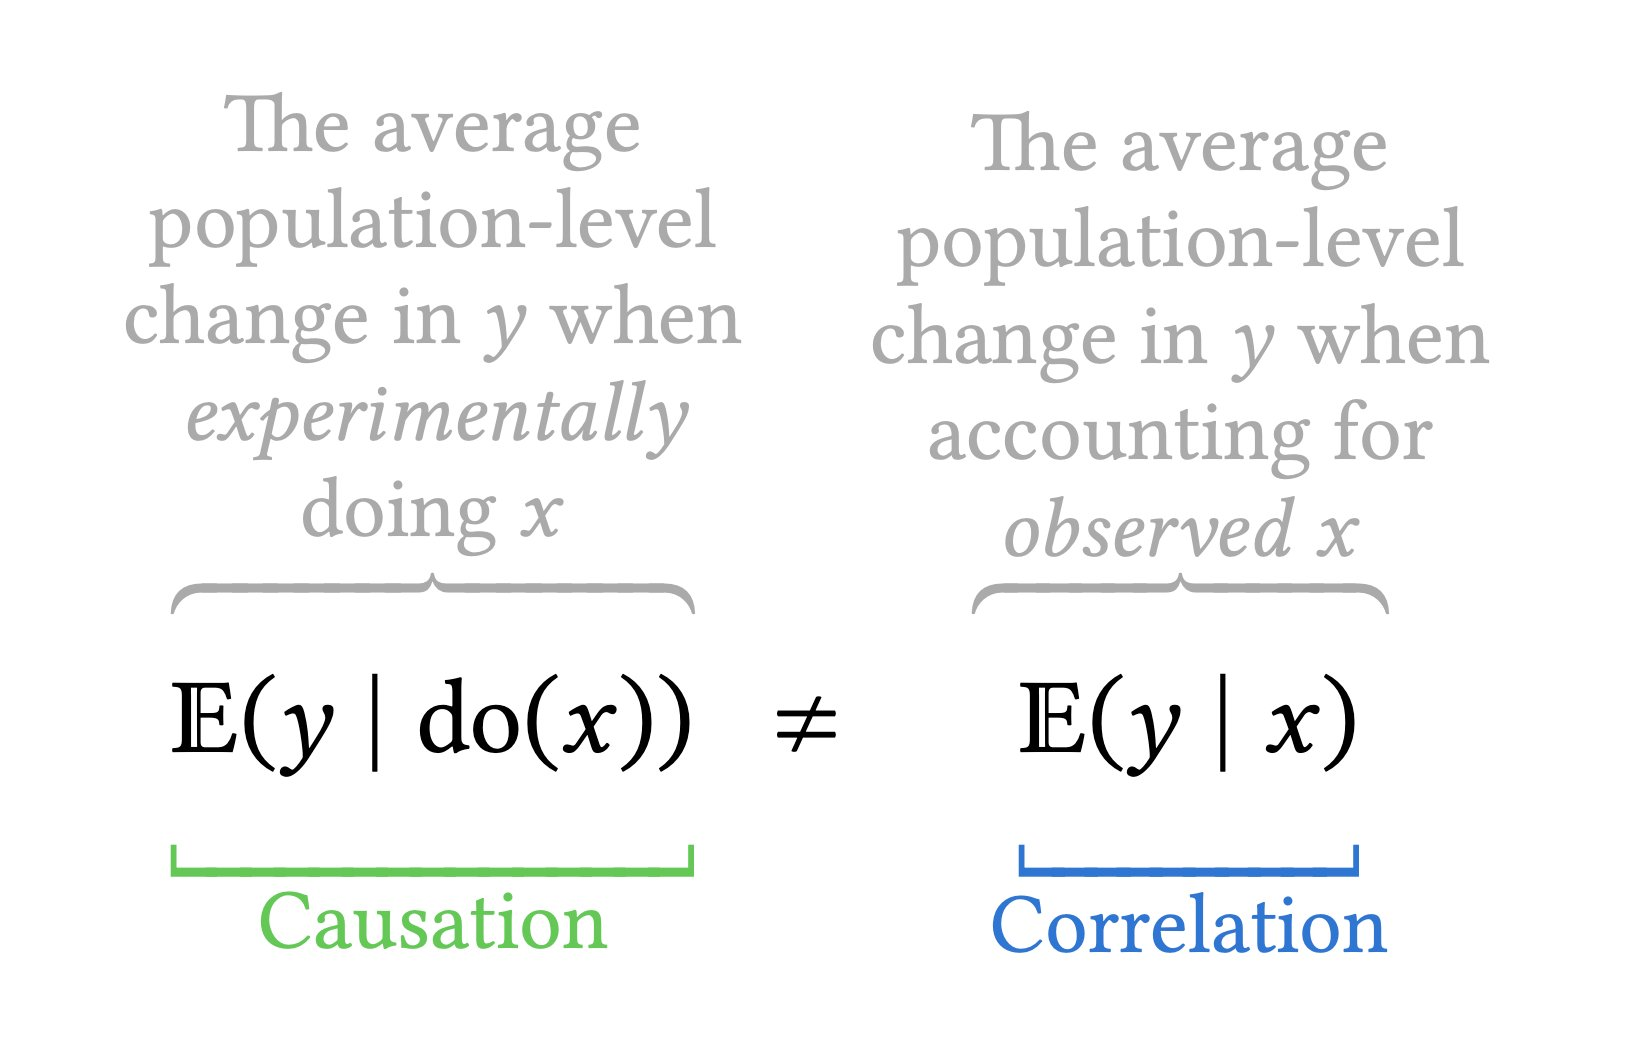
\includegraphics[width=0.85\textwidth,height=\textheight]{images/correlation_causation.jpg}

}

\caption{Difference between experimental and observational studies by
Andrew Heiss \href{https://creativecommons.org/licenses/by/4.0/}{CC-BY
4.0}}

\end{figure}%

\subsection{Continuous explanatories}\label{continuous-explanatories}

Continuous explanatories are typically specified by including a single
linear term, leading to the simple linear regression of the form
\(Y \mid X=x \sim \mathsf{normal}(\beta_0 + \beta x, \sigma^2)\). In
this situation \(\beta_0\) is the intercept (the mean value of \(Y\)
when \(x=0\)) and \(\beta_1\) is the slope, i.e., the average increase
of \(Y\) when \(x\) increases by one unit. Figure~\ref{fig-droitenuage}
shows such an example of a model with a single explanatory. As revealed
by the exploratory data analysis of
Example~\ref{exm-college-salary-discrimination}, this model is
simplistic and clearly insufficient to explain differences in salary.

\begin{figure}[ht!]

\centering{

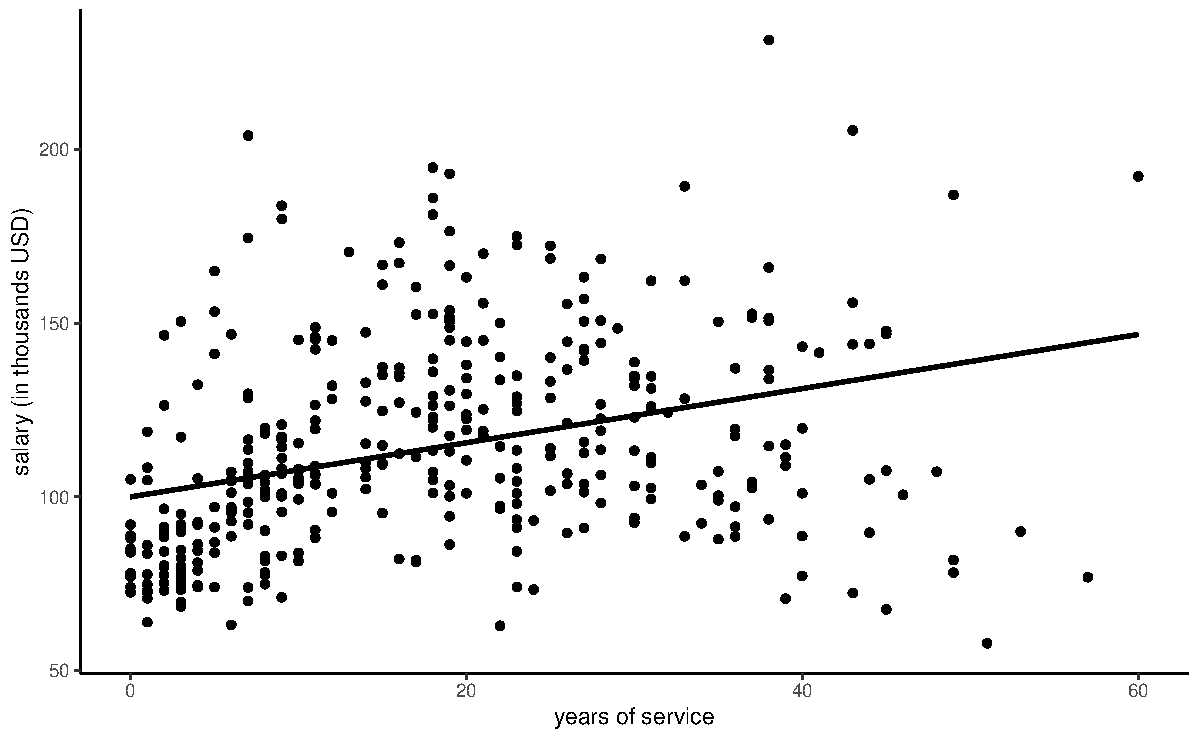
\includegraphics[width=0.85\textwidth,height=\textheight]{linearmodels_files/figure-pdf/fig-droitenuage-1.pdf}

}

\caption{\label{fig-droitenuage}Simple linear regression model for the
salary of professors as a function of the number of years of service.}

\end{figure}%

The \textbf{intercept} \(\beta_0\) is the value when all of
\(x_1, \ldots, x_p\) are zero. The interpretation of the other mean
parameters in the model depends crucially on the parametrization and on
potential interactions or higher order terms.

Rather, a more interesting perspective considers the effect of an
increase of an explanatory variable. If
\(\mu=\mathbf{x}\boldsymbol{\beta}\) and each, then a one unit increase
of the \(j\) component \((j=1, \ldots, p)\) leads to a change of
\(\partial \mu/\partial x_j\).

Generally, we can increase \(X_j\) by one unit and compare the increase
in the mean, here for \(X_j\) \begin{align*}
\mathsf{E}(Y \mid X_j=x_j+1, \boldsymbol{X}_{-j} = \boldsymbol{x}_{-j}) - \mathsf{E}(Y \mid X_j=x_j, \boldsymbol{X}_{-j} = \boldsymbol{x}_{-j}) = \beta_j.
\end{align*}

If the relationship between explanatory \(X\) and response \(Y\), as
assessed from a scatterplot, is not linear, we may consider more
complicated function of the explanatories, as Example~\ref{exm-auto}
shows.

\begin{example}[Quadratic curve fo the automobile
data]\protect\hypertarget{exm-auto}{}\label{exm-auto}

We consider a linear regression model for the fuel autonomy of cars as a
function of the power of their motor (measured in horsepower) from the
\texttt{auto} dataset. The postulated model, \begin{align*}
\texttt{mpg}_i = \beta_0 + \beta_1 \texttt{horsepower}_i + \beta_2 \texttt{horsepower}_i^2 + \varepsilon_i,
\end{align*} includes a quadratic term. Figure~\ref{fig-autoquad2d}
shows the scatterplot with the fitted regression line, above which the
line for the simple linear regression for horsepower is added. The
marginal effect of an increase of one unit in \texttt{horsepower} is
\(\beta_1 + 2\beta_2 \texttt{horsepower}\), which depends on the value
of the explanatory.

To fit higher order polynomials, we use the \texttt{poly} as the latter
leads to more numerical stability. For general transformations, the
\texttt{I} function tells the software interpret the input ``as is''.
Thus, \texttt{lm(y\textasciitilde{}x+I(x\^{}2))}, would fit a linear
model with design matrix
\([\boldsymbol{1}_n\, \mathbf{x}\, \mathbf{x}^2]\).

\begin{figure}[ht!]

\centering{

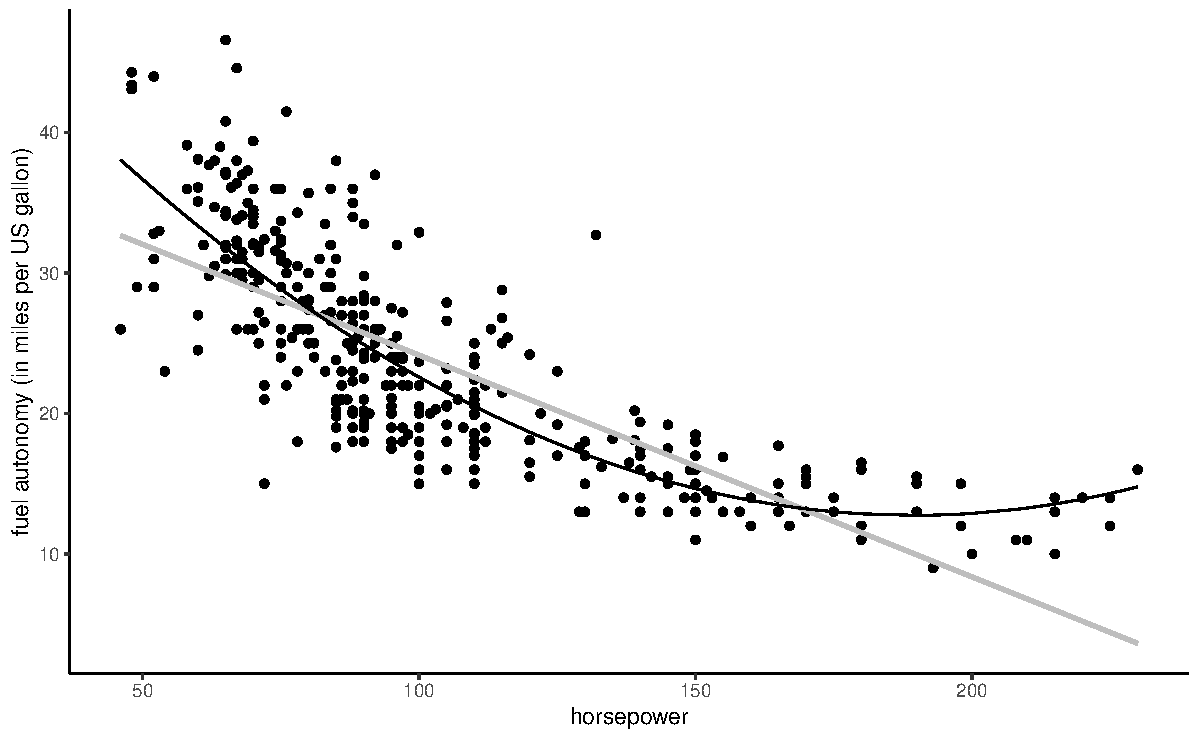
\includegraphics[width=0.85\textwidth,height=\textheight]{linearmodels_files/figure-pdf/fig-autoquad2d-1.pdf}

}

\caption{\label{fig-autoquad2d}Linear regression models for the fuel
autonomy of cars as a function of motor power.}

\end{figure}%

It appears graphically that the quadratic model fits better than the
simple linear alternative: we will assess this hypothesis formally
later. For the degree two polynomial, Figure~\ref{fig-autoquad2d} show
that fuel autonomy decreases rapidly when power increases between 50 to
100, then more slow until 189.35 hp. After that, the model postulates
that autonomy increases again as evidenced by the scatterplot, but
beware of extrapolating (weird things can happen beyond the range of the
data, as exemplified by
\href{https://web.archive.org/web/20210315050023/https://livefreeordichotomize.com/2020/05/05/model-detective/}{Hassett's
cubic model for the number of daily cases of Covid19 in the USA}).

The representation in Figure~\ref{fig-autoquad2d} may seem
counter-intuitive given that we fit a linear model, but it is a 2D
projection of 3D coordinates for the equation
\(\beta_0 + \beta_1x-y +\beta_2z =0\), where \(x=\texttt{horsepower}\),
\(z=\texttt{horsepower}^2\) and \(y=\texttt{mpg}\). Physics and common
sense force \(z = x^2\), and so the fitted values lie on a curve in a 2D
subspace of the fitted plan, as shown in grey in the three-dimensional
Figure~\ref{fig-hyperplan}.

\begin{figure}[ht!]

\centering{

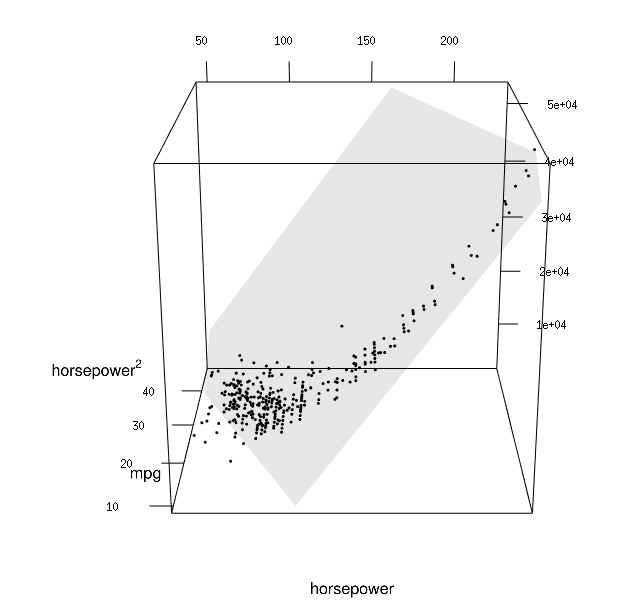
\includegraphics[width=0.85\textwidth,height=\textheight]{images/hyperplane_auto.png}

}

\caption{\label{fig-hyperplan}3D graphical representation of the linear
regression model for the \texttt{auto} data.}

\end{figure}%

\end{example}

\begin{refremark}[Discretization of continuous covariates]
Another option is to transform a continuous variable \(X\) into a
categorical variable by discretizing into bins and fitting a
piecewise-linear function of \(X\). The prime example of such option is
treating a Likert scale as a categorical variable. While this allows one
to fit more flexible functional relations between \(X\) and \(Y\), this
comes at the cost of additional coefficients for the same estimation
budget (fewer observations to estimate the effect of \(X\) results in
lower precision of the coefficients).

\begin{figure}[ht!]

\centering{

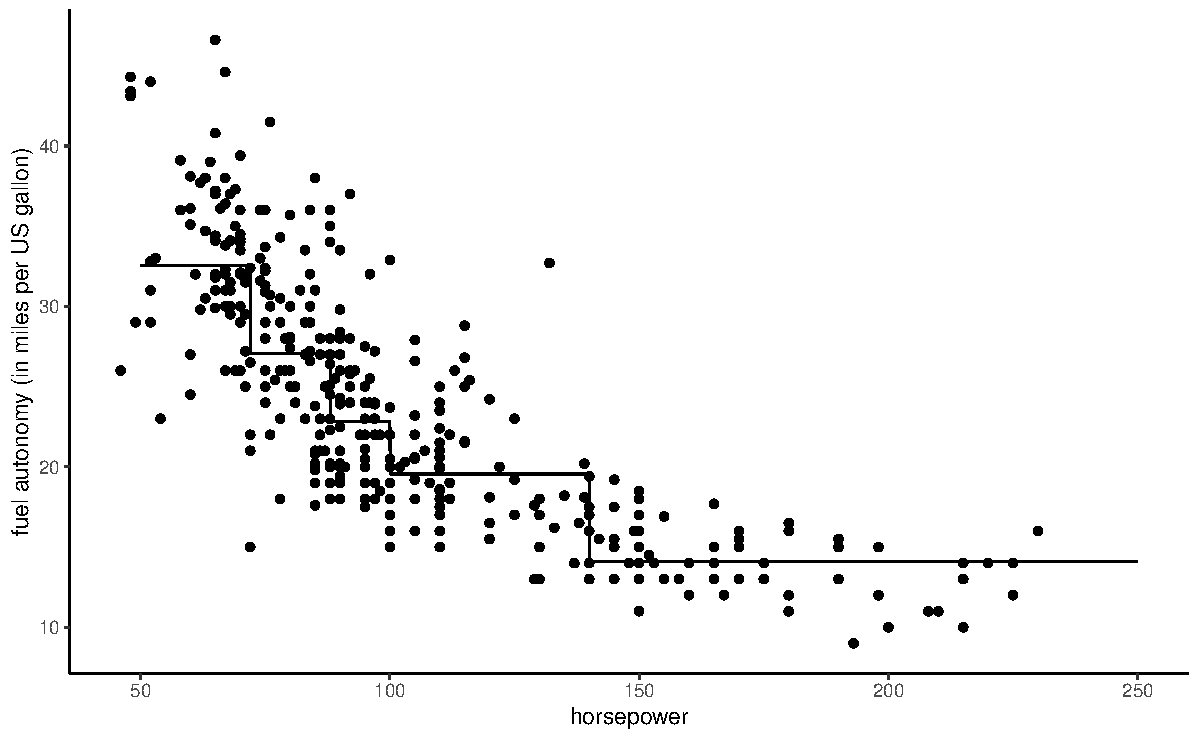
\includegraphics[width=0.85\textwidth,height=\textheight]{linearmodels_files/figure-pdf/fig-auto-discre-1.pdf}

}

\caption{\label{fig-auto-discre}Piecewise-linear model for the fuel
autonomy of cars as a function of motor power.}

\end{figure}%

\label{rem-discretization}

\end{refremark}

\subsection{Categorical covariates}\label{categorical-covariates}

Dummies are variables (columns of explanatories from the model matrix)
which only include \(-1\), \(0\) and \(1\) to give indicator of the
level of groups. For a binary outcome, we can create a column that has
entries \(1\) for the treatment and \(0\) for the control group.

\begin{example}[Linear models with a single binary
variable]\protect\hypertarget{exm-moon}{}\label{exm-moon}

Moon and VanEpps (\citeproc{ref-Moon.VanEpps:2023}{2023}) consider the
impact of providing suggested amounts for donations to a charity (as
opposed to an open-ended request). In Study 1, participants were given
the chance of winning 25\$ and giving part of this amount to charity.

Consider for example a linear model that includes the \texttt{amount}
(in dollars, from 0 for people who did not donate, up to 25 dollars). We
fit a model as a function of
\begin{align*}\texttt{condition} = \begin{cases} 0 , & \text{open-ended},\\
1, & \text{suggested quantity}
\end{cases}
\end{align*} The equation of the simple linear model that includes the
binary variable \texttt{condition} is \begin{align*}
\mathsf{E}(\texttt{amount} \mid \texttt{condition})&= \beta_0 + \beta_1 \mathbf{1}_{\texttt{condition}=\texttt{quantity}}.
\\&= \begin{cases}
\beta_0, & \texttt{condition}=0, \\
\beta_0 + \beta_1 & \texttt{condition}=1.
\end{cases}
\end{align*} Let \(\mu_0\) denote the theoretical average amount for the
open-ended amount and \(\mu_1\) that of participants of the treatment
\texttt{quantity} group. We can write the equation for the conditional
expectation for each experimental \texttt{condition}

A linear model that only contains a binary variable \(X\) as regressor
amounts to specifying a different mean for each of two groups: the
average of the treatment group is \(\beta_0 + \beta_1 = \mu_1\) and
\(\beta_1=\mu_1-\mu_0\) represents the difference between the average
donation amount of people given \texttt{open-ended} amounts and those
who are offered suggested amounts (\texttt{quantity}), including zeros
for the amount of people who did not donate. The parametrization of the
linear model with \(\beta_0\) and \(\beta_1\) is in terms of pairwise
differences relative to the baseline category and is particularly useful
if we want to test for mean difference between the groups, as this
amounts to testing \(\mathscr{H}_0: \beta_1=0\).

\begin{figure}[ht!]

\centering{

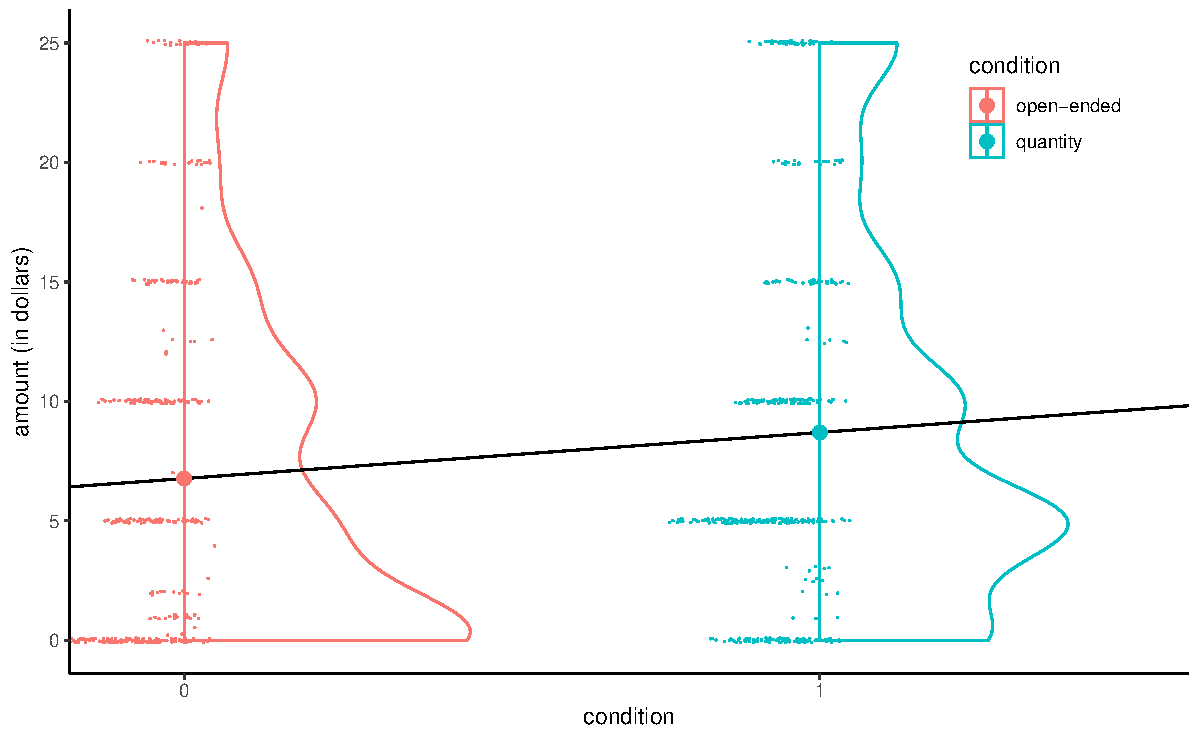
\includegraphics[width=0.85\textwidth,height=\textheight]{linearmodels_files/figure-pdf/fig-donation-moon-1.pdf}

}

\caption{\label{fig-donation-moon}Simple linear model for the
\texttt{MV23\_S1} data using the binary variable \texttt{condition} as
explanatory even if the equation defines a line, only its values in
\(0/1\) are realistic.}

\end{figure}%

Even if the linear model defines a line, the latter is only meaningful
when evaluated at \(0\) or \(1\); Figure~\ref{fig-donation-moon} shows
it in addition to sample observations (jittered horizontally) and a
density estimate for each condition. The colored dot represents the
mean, which will coincide with the estimates.

It is clear that the data are heavily discretized, with lots of ties and
zeros. However, given the sample size of 869 observations, we can easily
draw conclusions in each group.

\end{example}

Let us consider categorical variables with \(K > 2\) levels, which in
\textbf{R} are of class \texttt{factor}. The default parametrization for
factors are in terms of treatment contrast: the reference level of the
factor (by default, the first value in alphanumerical order) will be
treated as the reference category and assimilated to the intercept. The
software will then create a set of \(K-1\) dummy variables for a factor
with \(K\) levels, each of which will have ones for the relevant value
and zero otherwise.

\begin{example}[Dummy coding for categorical
variables]\protect\hypertarget{exm-baumann-dummies}{}\label{exm-baumann-dummies}

Consider the Baumann, Seifert-Kessell, and Jones
(\citeproc{ref-Baumann:1992}{1992}) study and the sole inclusion of the
\texttt{group} variable. The data are ordered by group: the first 22
observations are for group \texttt{DR}, the 22 next ones for group
\texttt{DRTA} and the last 22 for \texttt{TA}. If we fit a model with
\texttt{group} as categorical variables

\begin{Shaded}
\begin{Highlighting}[]
\FunctionTok{class}\NormalTok{(BSJ92}\SpecialCharTok{$}\NormalTok{group) }\CommentTok{\# Check that group is a factor}
\CommentTok{\#\textgreater{} [1] "factor"}
\FunctionTok{levels}\NormalTok{(BSJ92}\SpecialCharTok{$}\NormalTok{group) }\CommentTok{\# First level shown is reference}
\CommentTok{\#\textgreater{} [1] "DR"   "DRTA" "TA"}
\CommentTok{\# Print part of the model matrix }
\CommentTok{\# (three individuals from different groups)}
\FunctionTok{model.matrix}\NormalTok{(}\SpecialCharTok{\textasciitilde{}}\NormalTok{ group, }\AttributeTok{data =}\NormalTok{ BSJ92)[}\FunctionTok{c}\NormalTok{(}\DecValTok{1}\NormalTok{,}\DecValTok{23}\NormalTok{,}\DecValTok{47}\NormalTok{),]}
\CommentTok{\#\textgreater{}    (Intercept) groupDRTA groupTA}
\CommentTok{\#\textgreater{} 1            1         0       0}
\CommentTok{\#\textgreater{} 23           1         1       0}
\CommentTok{\#\textgreater{} 47           1         0       1}
\CommentTok{\# Compare with levels of factors recorded}
\NormalTok{BSJ92}\SpecialCharTok{$}\NormalTok{group[}\FunctionTok{c}\NormalTok{(}\DecValTok{1}\NormalTok{,}\DecValTok{23}\NormalTok{,}\DecValTok{47}\NormalTok{)]}
\CommentTok{\#\textgreater{} [1] DR   DRTA TA  }
\CommentTok{\#\textgreater{} Levels: DR DRTA TA}
\end{Highlighting}
\end{Shaded}

The mean model specification is
\[\mathsf{E}(Y \mid \texttt{group})= \beta_0 + \beta_1\mathbf{1}_{\texttt{group}=\texttt{DRTA}} + \beta_2\mathbf{1}_{\texttt{group}=\texttt{TA}}.\]
Since the variable \texttt{group} is categorical with \(K=3\) levels, we
need \(K-1 = 2\) dummy explanatories to include the effect and obtain
one average per group. With the default parametrization, we obtain

\begin{itemize}
\tightlist
\item
  \(\mathbf{1}_{\texttt{group}=\texttt{DRTA}}=1\) if \texttt{group=DRTA}
  and zero otherwise.
\item
  \(\mathbf{1}_{\texttt{group}=\texttt{TA}}=1\) if \texttt{group=TA} and
  zero otherwise.
\end{itemize}

Because the model includes an intercept and the model ultimately
describes three group averages, we only need two additional variables.
With the treatment parametrization, the group mean of the reference
group equals the intercept coefficient, \(\mu_{\texttt{DR}}=\beta_0\),

\begin{longtable}[]{@{}lrrr@{}}

\caption{\label{tbl-dummies-tr}Parametrization of dummies for a
categorical variable with the default treatment contrasts.}

\tabularnewline

\toprule\noalign{}
& (Intercept) & groupDRTA & groupTA \\
\midrule\noalign{}
\endhead
\bottomrule\noalign{}
\endlastfoot
DR & 1 & 0 & 0 \\
DRTA & 1 & 1 & 0 \\
TA & 1 & 0 & 1 \\

\end{longtable}

When \texttt{group}=\texttt{DR} (baseline), both indicator variables
\texttt{groupDRTA} and \texttt{groupTA} are zero. The average in each
group is \(\mu_{\texttt{DR}} = \beta_0\),
\(\mu_{\texttt{DRTA}}=\beta_0 + \beta_1\) and
\(\mu_{\texttt{TA}} = \beta_0 + \beta_2\). We thus find that \(\beta_1\)
is the difference in mean between group \texttt{DRTA} and group
\texttt{DR}, and similarly
\(\beta_2=\mu_{\texttt{TA}}- \mu_{\texttt{DR}}\).

\end{example}

\begin{refremark}[Sum-to-zero constraints]
The parametrization discussed above, which is the default for the
\texttt{lm} function, isn't the only one available. We consider an
alternative ones: rather than comparing each group mean with that of a
baseline category, the default parametrization for analysis of variance
models is in terms of sum-to-zero constraints, whereby the intercept is
the equiweighted average of every group, and the parameters
\(\beta_1, \ldots, \beta_{K-1}\) are differences to this average.

\begin{Shaded}
\begin{Highlighting}[]
\FunctionTok{model.matrix}\NormalTok{(}
    \SpecialCharTok{\textasciitilde{}}\NormalTok{ group, }
    \AttributeTok{data =}\NormalTok{ BSJ92, }
    \AttributeTok{contrasts.arg =} \FunctionTok{list}\NormalTok{(}\AttributeTok{group =} \StringTok{"contr.sum"}\NormalTok{))}
\end{Highlighting}
\end{Shaded}

\begin{longtable}[]{@{}lrrr@{}}

\caption{\label{tbl-sum2zero}Parametrization of dummies for the
sum-to-zero constraints for a categorical variable.}

\tabularnewline

\toprule\noalign{}
& (Intercept) & group1 & group2 \\
\midrule\noalign{}
\endhead
\bottomrule\noalign{}
\endlastfoot
DR & 1 & 1 & 0 \\
DRTA & 1 & 0 & 1 \\
TA & 1 & -1 & -1 \\

\end{longtable}

In the sum-to-zero constraint, we again only get two dummy variables,
labelled \texttt{group1} and \texttt{group2}, along with the intercept.
The value of \texttt{group1} is \(1\) if \texttt{group=DR}, \(0\) if
\texttt{group=DRTA} and \(-1\) if \texttt{group=TA}. Using the
invariance property, we find \(\mu_{\texttt{DR}} = \beta_0 + \beta_1\),
\(\mu_{\texttt{DRTA}}=\beta_0 + \beta_2 \beta_1\) and
\(\mu_{\texttt{TA}} = \beta_0 - \beta_1 - \beta_2\) (more generally, the
intercept minus the sum of all the other mean coefficients). Some
algebraic manipulation reveals that
\(\beta_0 = (\mu_{\texttt{DR}} +\mu_{\texttt{DRTA}}+\mu_{\texttt{TA}})/3\).

If we removed the intercept, then we could include three dummies for
each treatment group and each parameter would correspond to the average.
This isn't recommended in \textbf{R} because the software treats models
without the intercept differently and some output will be nonsensical
(e.g., the coefficient of determination will be wrong).

\label{rem-sumtozero}

\end{refremark}

\begin{example}[]\protect\hypertarget{exm-interpretation1}{}\label{exm-interpretation1}

We consider a pre-post model for the error detection task test of
Baumann, Seifert-Kessell, and Jones (\citeproc{ref-Baumann:1992}{1992}).
We fit a linear model with the pre-test score and the experimental
condition.

\begin{Shaded}
\begin{Highlighting}[]
\FunctionTok{data}\NormalTok{(BSJ92, }\AttributeTok{package =} \StringTok{"hecedsm"}\NormalTok{) }\CommentTok{\#load data}
\FunctionTok{str}\NormalTok{(BSJ92) }\CommentTok{\# Check that categorical variables are factors}
\CommentTok{\#\textgreater{} tibble [66 x 6] (S3: tbl\_df/tbl/data.frame)}
\CommentTok{\#\textgreater{}  $ group    : Factor w/ 3 levels "DR","DRTA","TA": 1 1 1 1 1 1 1 1 1 1 ...}
\CommentTok{\#\textgreater{}  $ pretest1 : int [1:66] 4 6 9 12 16 15 14 12 12 8 ...}
\CommentTok{\#\textgreater{}  $ pretest2 : int [1:66] 3 5 4 6 5 13 8 7 3 8 ...}
\CommentTok{\#\textgreater{}  $ posttest1: int [1:66] 5 9 5 8 10 9 12 5 8 7 ...}
\CommentTok{\#\textgreater{}  $ posttest2: int [1:66] 4 5 3 5 9 8 5 5 7 7 ...}
\CommentTok{\#\textgreater{}  $ posttest3: int [1:66] 41 41 43 46 46 45 45 32 33 39 ...}
\CommentTok{\# Check summary statistics for posttest1}
\NormalTok{BSJ92 }\SpecialCharTok{|\textgreater{}} \CommentTok{\# compute group average}
   \FunctionTok{group\_by}\NormalTok{(group) }\SpecialCharTok{|\textgreater{}} 
   \FunctionTok{summarize}\NormalTok{(}\AttributeTok{mean\_pre =} \FunctionTok{mean}\NormalTok{(pretest1),}
             \AttributeTok{mean\_post =} \FunctionTok{mean}\NormalTok{(posttest1),}
             \AttributeTok{diff\_impr =}\NormalTok{ mean\_post }\SpecialCharTok{{-}}\NormalTok{ mean\_pre) }
\CommentTok{\#\textgreater{} \# A tibble: 3 x 4}
\CommentTok{\#\textgreater{}   group mean\_pre mean\_post diff\_impr}
\CommentTok{\#\textgreater{}   \textless{}fct\textgreater{}    \textless{}dbl\textgreater{}     \textless{}dbl\textgreater{}     \textless{}dbl\textgreater{}}
\CommentTok{\#\textgreater{} 1 DR       10.5       6.68   {-}3.82  }
\CommentTok{\#\textgreater{} 2 DRTA      9.73      9.77    0.0455}
\CommentTok{\#\textgreater{} 3 TA        9.14      7.77   {-}1.36}
\CommentTok{\# Fit the ANOVA for the difference}
\NormalTok{linmod1 }\OtherTok{\textless{}{-}} \FunctionTok{lm}\NormalTok{(}
\NormalTok{   posttest1 }\SpecialCharTok{{-}}\NormalTok{ pretest1 }\SpecialCharTok{\textasciitilde{}}\NormalTok{ group, }
   \AttributeTok{data =}\NormalTok{ BSJ92)}
\FunctionTok{coef}\NormalTok{(linmod1) }\CommentTok{\# Mean model coefficients}
\CommentTok{\#\textgreater{} (Intercept)   groupDRTA     groupTA }
\CommentTok{\#\textgreater{}       {-}3.82        3.86        2.45}
\CommentTok{\# Fit a linear regression}
\NormalTok{linmod2 }\OtherTok{\textless{}{-}} \FunctionTok{lm}\NormalTok{(}
\NormalTok{   posttest1 }\SpecialCharTok{\textasciitilde{}}\NormalTok{ pretest1 }\SpecialCharTok{+}\NormalTok{ group, }
   \AttributeTok{data =}\NormalTok{ BSJ92 }\SpecialCharTok{|\textgreater{}} 
\NormalTok{      dplyr}\SpecialCharTok{::}\FunctionTok{mutate}\NormalTok{( }\CommentTok{\# mean{-}center pretest result}
        \AttributeTok{pretest1 =}\NormalTok{ pretest1 }\SpecialCharTok{{-}} \FunctionTok{mean}\NormalTok{(pretest1)))}
\FunctionTok{coef}\NormalTok{(linmod2) }\CommentTok{\# Mean model coefficients}
\CommentTok{\#\textgreater{} (Intercept)    pretest1   groupDRTA     groupTA }
\CommentTok{\#\textgreater{}       6.188       0.693       3.627       2.036}
\end{Highlighting}
\end{Shaded}

With the ANOVA model for the group as a function of the improvement and
using the default treatment parameterization,, the intercept is the
average of post-test minus pre-test score for group \texttt{DR}, and the
other two coefficients are the difference between groups \texttt{DRTA}
and \texttt{DR}, and the difference between groups \texttt{TA} and
\texttt{DR}. Thus, the higher average improvement is for \texttt{DRTA},
then \texttt{TA}, then the baseline \texttt{DR}.

Consider next a linear model in which we allow the post-test score to be
a linear function of the pre-test. we find that, for each point score on
the pre-test, the post-test score increases by 0.693 marks regardless of
the group. The \texttt{DRTA} group (respectively \texttt{TA}) has an
average, ceteris paribus, that is 3.627 (respectively 2.036) points
higher than that of the baseline group \texttt{DR} for two people with
the same pre-test score. Because we centered the continuous covariate
\texttt{pretest1}, the intercept \(\beta_0\) is the average post-test
score of a person from the \texttt{DR} group who scored the overall
average of all 66 students in the pre-test.

\end{example}

\begin{example}[Wage inequality in an American
college]\protect\hypertarget{exm-gender-disparity}{}\label{exm-gender-disparity}

We consider a linear regression model for the \texttt{college} data that
includes sex, academic rank, field of study and the number of years of
service as explanatories.

The postulated model is \begin{align*}
\texttt{salary} &= \beta_0 + \beta_1 \texttt{sex}_{\texttt{woman}} +\beta_2 \texttt{field}_{\texttt{theoretical}} \\&\quad +\beta_3 \texttt{rank}_{\texttt{associate}}
+\beta_4 \texttt{rank}_{\texttt{full}}  +\beta_5 \texttt{service} + \varepsilon.
\end{align*}

\begin{longtable}[]{@{}
  >{\raggedleft\arraybackslash}p{(\columnwidth - 10\tabcolsep) * \real{0.1667}}
  >{\raggedleft\arraybackslash}p{(\columnwidth - 10\tabcolsep) * \real{0.1667}}
  >{\raggedleft\arraybackslash}p{(\columnwidth - 10\tabcolsep) * \real{0.1667}}
  >{\raggedleft\arraybackslash}p{(\columnwidth - 10\tabcolsep) * \real{0.1667}}
  >{\raggedleft\arraybackslash}p{(\columnwidth - 10\tabcolsep) * \real{0.1667}}
  >{\raggedleft\arraybackslash}p{(\columnwidth - 10\tabcolsep) * \real{0.1667}}@{}}
\caption{Estimated coefficients of the linear model for the
\(\texttt{college}\) (in USD, rounded to the nearest
dollar).}\tabularnewline
\toprule\noalign{}
\begin{minipage}[b]{\linewidth}\raggedleft
\(\widehat{\beta}_0\)
\end{minipage} & \begin{minipage}[b]{\linewidth}\raggedleft
\(\widehat{\beta}_1\)
\end{minipage} & \begin{minipage}[b]{\linewidth}\raggedleft
\(\widehat{\beta}_2\)
\end{minipage} & \begin{minipage}[b]{\linewidth}\raggedleft
\(\widehat{\beta}_3\)
\end{minipage} & \begin{minipage}[b]{\linewidth}\raggedleft
\(\widehat{\beta}_4\)
\end{minipage} & \begin{minipage}[b]{\linewidth}\raggedleft
\(\widehat{\beta}_5\)
\end{minipage} \\
\midrule\noalign{}
\endfirsthead
\toprule\noalign{}
\begin{minipage}[b]{\linewidth}\raggedleft
\(\widehat{\beta}_0\)
\end{minipage} & \begin{minipage}[b]{\linewidth}\raggedleft
\(\widehat{\beta}_1\)
\end{minipage} & \begin{minipage}[b]{\linewidth}\raggedleft
\(\widehat{\beta}_2\)
\end{minipage} & \begin{minipage}[b]{\linewidth}\raggedleft
\(\widehat{\beta}_3\)
\end{minipage} & \begin{minipage}[b]{\linewidth}\raggedleft
\(\widehat{\beta}_4\)
\end{minipage} & \begin{minipage}[b]{\linewidth}\raggedleft
\(\widehat{\beta}_5\)
\end{minipage} \\
\midrule\noalign{}
\endhead
\bottomrule\noalign{}
\endlastfoot
86596 & -4771 & -13473 & 14560 & 49160 & -89 \\
\end{longtable}

The interpretation of the coefficients is as follows:

\begin{itemize}
\tightlist
\item
  The estimated intercept is \(\widehat{\beta}_0=86596\) dollars; it
  corresponds to the mean salary of men assistant professors who just
  started the job and works in an applied domain.
\item
  everything else being equal (same field, academic rank, and number of
  years of service), the estimated salary difference between a woman and
  is estimated at \(\widehat{\beta}_1=-4771\) dollars.
\item
  \emph{ceteris paribus}, the salary difference between a professor
  working in a theoretical field and one working in an applied field is
  \(\beta_2\) dollars: our estimate of this difference is \(-13473\)
  dollars, meaning applied pays more than theoretical.
\item
  \emph{ceteris paribus}, the estimated mean salary difference between
  associate and assistant professors is \(\widehat{\beta}_3=14560\)
  dollars.
\item
  \emph{ceteris paribus}, the estimated mean salary difference between
  full and assistant professors is \(\widehat{\beta}_4=49160\) dollars.
\item
  within the same academic rank, every additional year of service leads
  to a mean salary increase of \(\widehat{\beta}_5=-89\) dollars.
\end{itemize}

\end{example}

\section{Parameter estimation}\label{parameter-estimation}

The linear model includes \(p+1\) mean parameters and a standard
deviation \(\sigma\), which is assumed constant for all observations.

\subsection{Ordinary least squares estimator}\label{ols}

Given a design or model matrix \(\mathbf{X}\) and a linear model
formulation \(\mathsf{E}(Y_i) = \mathbf{x}_i\boldsymbol{\beta}\), we can
try to find the parameter vector
\(\boldsymbol{\beta} \in \mathbb{R}^{p+1}\) that minimizes the mean
squared error, i.e., the average squared vertical distance between the
fitted values \(\widehat{y}_i=\mathbf{x}_i\widehat{\boldsymbol{\beta}}\)
and the observations \(y_i\).

\begin{figure}[ht!]

\centering{

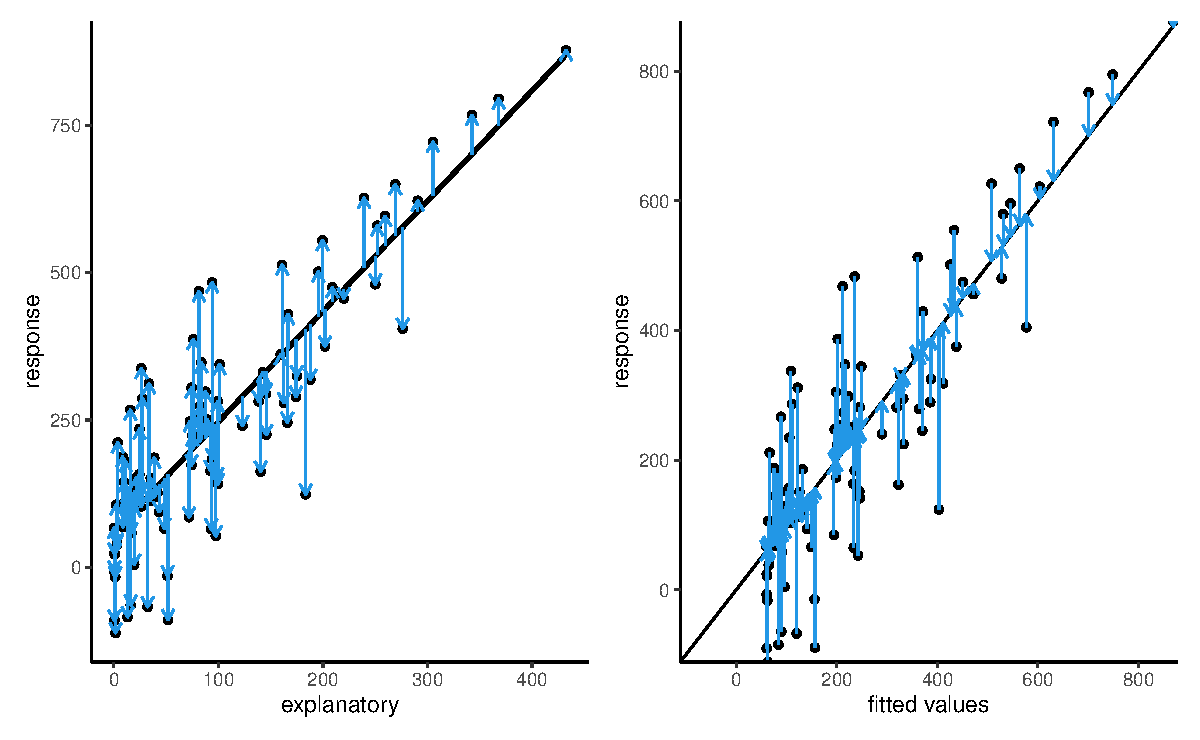
\includegraphics[width=0.85\textwidth,height=\textheight]{linearmodels_files/figure-pdf/fig-vertdist-1.pdf}

}

\caption{\label{fig-vertdist}Ordinary residuals \(e_i\) (vertical
vectors) added to the regression line in the scatter \((x, y)\) (left)
and the fit of response \(y_i\) against fitted values \(\widehat{y}_i\).
The ordinary least squares line minimizes the average squared length of
the ordinary residuals.}

\end{figure}%

\begin{proposition}[Ordinary least
squares]\protect\hypertarget{prp-ols-mle}{}\label{prp-ols-mle}

Consider the optimization problem \begin{align*}
\widehat{\boldsymbol{\beta}}&=\mathrm{arg min}_{\boldsymbol{\beta} \in \mathbb{R}^{p+1}}\sum_{i=1}^n (y_i-\mathbf{x}_i\boldsymbol{\beta})^2
\\&=(\boldsymbol{y}-\mathbf{X}\boldsymbol{\beta})^\top(\boldsymbol{y}-\mathbf{X}\boldsymbol{\beta}).
\end{align*} We can compute the derivative of the right hand side with
respect to \(\boldsymbol{\beta}\), set it to zero and solve for
\(\widehat{\boldsymbol{\beta}}\), \begin{align*}
\mathbf{0}_n&=\frac{\partial}{\partial\boldsymbol{\beta}}(\boldsymbol{y}-\mathbf{X}\boldsymbol{\beta})^\top(\boldsymbol{y}-\mathbf{X}\boldsymbol{\beta})\\
\\&=\frac{\partial (\boldsymbol{y}-\mathbf{X}\boldsymbol{\beta})}{\partial \boldsymbol{\beta}}\frac{\partial (\boldsymbol{y}-\mathbf{X}\boldsymbol{\beta})^\top(\boldsymbol{y}-\mathbf{X}\boldsymbol{\beta})}{\partial (\boldsymbol{y}-\mathbf{X}\boldsymbol{\beta})}\\
 \\&=2\mathbf{X}^\top (\boldsymbol{y}-\mathbf{X}\boldsymbol{\beta})
\end{align*} using the
\href{http://www.stat.rice.edu/~dobelman/notes_papers/math/Matrix.Calculus.AppD.pdf}{chain
rule}. Distributing the terms leads to the so-called \emph{normal
equation} \begin{align*}
 \mathbf{X}^\top \mathbf{X}\boldsymbol{\beta}&=\mathbf{X}^\top \boldsymbol{y}.
\end{align*} If the \(n \times p\) matrix \(\mathbf{X}\) is full-rank,
meaning that it's columns are not linear combinations of one another,
the quadratic form \(\mathbf{X}^\top \mathbf{X}\) is invertible and we
obtain the solution to the least square problems,
\begin{equation}\phantomsection\label{eq-ols}{
\widehat{\boldsymbol{\beta}} = \left(\mathbf{X}^\top \mathbf{X}\right)^{-1}\mathbf{X}^\top \boldsymbol{y}.
}\end{equation} This is the \textbf{ordinary least squares estimator}
(OLS). The explicit solution means that no numerical optimization is
needed for linear models.

\end{proposition}

We could also consider maximum likelihood estimation.
Proposition~\ref{prp-ols-mle} shows that, assuming normality of the
errors, the least square estimators of \(\boldsymbol{\beta}\) coincide
with the maximum likelihood estimator of \(\boldsymbol{\beta}\).

\begin{proposition}[Maximum likelihood estimation of the normal linear
model]\protect\hypertarget{prp-mle-normal-linmod}{}\label{prp-mle-normal-linmod}

The linear regression model specifies that the observations
\(Y_i \sim \mathsf{normal}(\mathbf{x}_i\boldsymbol{\beta}, \sigma^2)\)
are independent. The linear model has \(p+2\) parameters
(\(\boldsymbol{\beta}\) and \(\sigma^2\)) and the log likelihood is,
abstracting from constant terms, \begin{align*}
\ell(\boldsymbol{\beta}, \sigma)&\propto-\frac{n}{2} \ln (\sigma^2) -\frac{1}{2\sigma^2}\left\{(\boldsymbol{y}-\mathbf{X}\boldsymbol{\beta})^\top(\boldsymbol{y}-\mathbf{X}\boldsymbol{\beta})\right\}^2.
\end{align*} Maximizing the log likelihood with respect to
\(\boldsymbol{\beta}\) is equivalent to minimizing the sum of squared
errors \(\sum_{i=1}^n (y_i - \mathbf{x}_i\boldsymbol{\beta})^2\),
regardless of the value of \(\sigma\), and we recover the OLS estimator
\(\widehat{\boldsymbol{\beta}}\). The maximum likelihood estimator of
the variance \(\widehat{\sigma}^2\) is thus \begin{align*}
\widehat{\sigma}^2=\mathrm{arg max}_{\sigma^2} \ell(\widehat{\boldsymbol{\beta}}, \sigma^2).
\end{align*} The profile log likelihood for \(\sigma^2\), excluding
constant terms that don't depend on \(\sigma^2\), is \begin{align*}
\ell_{\mathrm{p}}(\sigma^2)
&\propto-\frac{1}{2}\left\{n\ln\sigma^2+\frac{1}{\sigma^2}(\boldsymbol{y}-\mathbf{X}\hat{\boldsymbol{\beta}})^\top(\boldsymbol{y}-\mathbf{X}\hat{\boldsymbol{\beta}})\right\}.
\end{align*} Differentiating each term with respect to \(\sigma^2\) and
setting the gradient equal to zero yields the maximum likelihood
estimator \begin{align*}
\widehat{\sigma}^2&=\frac{1}{n}(\boldsymbol{Y}-\mathbf{X}\hat{\boldsymbol{\beta}})^\top(\boldsymbol{Y}-\mathbf{X}\hat{\boldsymbol{\beta}})\\&= \frac{1}{n} \sum_{i=1}^n (y_i - \mathbf{x}_i\widehat{\boldsymbol{\beta}})^2\\&= \frac{\mathsf{SS}_e}{n};
\end{align*} where \(\mathsf{SS}_e\) is the sum of squared residuals.
The usual unbiased estimator of \(\sigma^2\) calculated by software is
\(S^2=\mathsf{SS}_e/(n-p-1)\), where the denominator is the sample size
\(n\) minus the number of mean parameters \(\boldsymbol{\beta}\),
\(p+1\).

\end{proposition}

\begin{refremark}[Invariance]
One direct consequence of likelihood estimation is that the fitted
values \(\widehat{y}_i\) for two model matrices \(\mathbf{X}_a\) and
\(\mathbf{X}_b\), are the same if they generate the same linear span, as
in Example~\ref{exm-baumann-dummies}. The interpretation of the
coefficients will however change. If we include an intercept term, then
we get the same output if the columns of explanatory are mean-centered.

\label{rem-invariance}

\end{refremark}

The value of \(\boldsymbol{\beta}\) is such that it will maximize the
correlation between \(Y\) and \(\widehat{Y}\). In the case of a single
categorical variable, we will obtain fitted values \(\widehat{y}\) that
correspond to the sample mean of each group.

\begin{refremark}[Geometry]
The vector of fitted values
\(\boldsymbol{y} =\mathbf{X} \widehat{\boldsymbol{\beta}} = \mathbf{H}_{\mathbf{X}}\boldsymbol{y}\)
is the projection of the response vector \(\boldsymbol{y}\) on the
linear span generated by the columns of \(\mathbf{X}\). The matrix
\(\mathbf{H}_{\mathbf{X}} = \mathbf{X}(\mathbf{X}^\top\mathbf{X})^{-1}\mathbf{X}^\top\),
often called hat matrix, is an orthogonal projection matrix, so
\(\mathbf{H}_{\mathbf{X}}=\mathbf{H}_{\mathbf{X}}^\top\) and
\(\mathbf{H}_{\mathbf{X}}\mathbf{H}_{\mathbf{X}} = \mathbf{H}_{\mathbf{X}}\)
and \(\mathbf{H}_{\mathbf{X}}\mathbf{X} = \mathbf{X}\). Since the vector
of residuals \(\boldsymbol{e} = (e_1, \ldots, e_n)^\top\), which appear
in the sum of squared errors, is defined as
\(\boldsymbol{y} - \widehat{\boldsymbol{y}}\) and
\(\widehat{\boldsymbol{y}}=\mathbf{X}\boldsymbol{\beta}\), simple
algebraic manipulations show that the inner product between ordinary
residuals and fitted values is zero, since \begin{align*}
\widehat{\boldsymbol{y}}^\top\boldsymbol{e} &= \widehat{\boldsymbol{\beta}}^\top \mathbf{X}^\top (\boldsymbol{y}- \mathbf{X} \widehat{\boldsymbol{\beta}})
\\&= \boldsymbol{y}^\top\mathbf{X}(\mathbf{X}^\top\mathbf{X})^{-1}\mathbf{X}^\top(\boldsymbol{y} - \mathbf{X}(\mathbf{X}^\top\mathbf{X})^{-1}\mathbf{X}^\top \boldsymbol{y})\\&=\boldsymbol{y}^\top\mathbf{H}_{\mathbf{X}}\boldsymbol{y} - \mathbf{X}(\mathbf{X}^\top\mathbf{X})^{-1}\mathbf{X}^\top\mathbf{X}(\mathbf{X}^\top\mathbf{X})^{-1}\mathbf{X}^\top \boldsymbol{y}
\\&= 0
\end{align*} where we use the definition of \(\widehat{\boldsymbol{y}}\)
and \(\boldsymbol{e} = \boldsymbol{y} - \widehat{\boldsymbol{y}}\) on
the first line, then substitute the OLS estimator
\(\widehat{\boldsymbol{\beta}} = (\mathbf{X}^\top\mathbf{X})^{-1}\mathbf{X}^\top\boldsymbol{y}\)
and distribute terms. Similarly,
\(\mathbf{X}^\top\boldsymbol{e}=\boldsymbol{0}_{p+1}\). The ordinary
residuals are thus orthogonal to both the model matrix \(\mathbf{X}\)
and to the fitted values.

A direct consequence of this fact is that the sample linear correlation
between \(\boldsymbol{e}\) and \(\widehat{\boldsymbol{y}}\) is zero; we
will use this property to build graphical diagnostics.

Since the inner product is zero, the mean of \(\boldsymbol{e}\) must be
zero provided that \(\mathbf{1}_n\) is in the linear span of
\(\mathbf{X}\).

\label{rem-geometry}

\end{refremark}

\begin{proposition}[Information matrix for normal linear regression
models]\protect\hypertarget{prp-info-normal}{}\label{prp-info-normal}

The entries of the observed information matrix of the normal linear
model are \begin{align*}
-\frac{\partial^2 \ell(\boldsymbol{\beta}, \sigma^2)}{\partial \boldsymbol{\beta}\partial \boldsymbol{\beta}^\top} &= \frac{1}{\sigma^2} \frac{\partial \mathbf{X}^\top(\boldsymbol{y}-\mathbf{X}\boldsymbol{\beta})}{\partial \boldsymbol{\beta}^\top} =  \frac{\mathbf{X}^\top\mathbf{X}}{\sigma^2}\\
-\frac{\partial^2 \ell(\boldsymbol{\beta}, \sigma^2)}{\partial \boldsymbol{\beta}\partial \sigma^2} &=- \frac{\mathbf{X}^\top(\boldsymbol{y}-\mathbf{X}\boldsymbol{\beta})}{\sigma^4}\\
-\frac{\partial^2 \ell(\boldsymbol{\beta}, \sigma^2)}{\partial (\sigma^2)^2} &= -\frac{n}{2\sigma^4} + \frac{(\boldsymbol{y}-\mathbf{X}\boldsymbol{\beta})^\top(\boldsymbol{y}-\mathbf{X}\boldsymbol{\beta})}{\sigma^6}.
\end{align*} If we evaluate the observed information at the MLE, we get
\begin{align*}
j(\widehat{\boldsymbol{\beta}}, \widehat{\sigma^2}) = 
\begin{pmatrix}
\frac{\mathbf{X}^\top\mathbf{X}}{\widehat{\sigma^2}} & \boldsymbol{0}_{p+1} \\  \boldsymbol{0}_{p+1}^\top & \frac{n}{2\widehat{\sigma^4}}
\end{pmatrix}
\end{align*} since \(\widehat{\sigma}^2=\mathsf{SS}_e/n\) and the
residuals are orthogonal to the model matrix. Since
\(\mathsf{E}(Y \mid \mathbf{X})=\mathbf{X}\boldsymbol{\beta}\), the
Fisher information is \begin{align*}
i(\boldsymbol{\beta}, \sigma^2) = 
\begin{pmatrix}
\frac{\mathbf{X}^\top\mathbf{X}}{\sigma^2} & \boldsymbol{0}_{p+1} \\  \boldsymbol{0}_{p+1}^\top & \frac{n}{2\sigma^4}
\end{pmatrix}
\end{align*} Since zero off-correlations in normal models amount to
independence, the MLE for \(\sigma^2\) and \(\boldsymbol{\beta}\) are
independent. Provided the \((p+1)\) square matrix
\(\mathbf{X}^\top\mathbf{X}\) is invertible, the large-sample variance
of the ordinary least squares estimator is
\(\sigma^2(\mathbf{X}^\top\mathbf{X})^{-1}\) and that of the MLE of the
variance is \(2\sigma^4/n\).

\end{proposition}

\subsection{Fitting linear models with
software}\label{fitting-linear-models-with-software}

Although we could build the model matrix ourselves and use the least
square formula of Equation~\ref{eq-ols}, the numerical routines
implemented in software are typically better behaved. The \texttt{lm}
function in \textbf{R} fits \textbf{linear models}, as does \texttt{glm}
with the default arguments. Objects of class \texttt{lm} have multiple
methods allow you to extract specific objects from \texttt{lm} objects.
For example, the functions \texttt{coef}, \texttt{resid},
\texttt{fitted}, \texttt{model.matrix} will return the coefficients
\(\widehat{\boldsymbol{\beta}},\) the ordinary residuals
\(\boldsymbol{e},\) the fitted values \(\widehat{\boldsymbol{y}}\) and
the model matrix \(\mathbf{X}\).

\begin{Shaded}
\begin{Highlighting}[]
\FunctionTok{data}\NormalTok{(BSJ92, }\AttributeTok{package =} \StringTok{"hecedsm"}\NormalTok{) }\CommentTok{\#load data}
\FunctionTok{str}\NormalTok{(BSJ92) }\CommentTok{\# Check that categorical variables are factors}
\CommentTok{\# Fit the linear regression}
\NormalTok{linmod }\OtherTok{\textless{}{-}} \FunctionTok{lm}\NormalTok{(posttest1 }\SpecialCharTok{\textasciitilde{}}\NormalTok{ pretest1 }\SpecialCharTok{+}\NormalTok{ group, }
             \AttributeTok{data =}\NormalTok{ BSJ92)}
\NormalTok{beta\_hat }\OtherTok{\textless{}{-}} \FunctionTok{coef}\NormalTok{(linmod) }\CommentTok{\# beta coefficients}
\NormalTok{vcov\_beta }\OtherTok{\textless{}{-}} \FunctionTok{vcov}\NormalTok{(linmod) }\CommentTok{\# Covariance matrix of betas}
\FunctionTok{summary}\NormalTok{(linmod) }\CommentTok{\# summary table}
\NormalTok{beta\_ci }\OtherTok{\textless{}{-}} \FunctionTok{confint}\NormalTok{(linmod) }\CommentTok{\# Wald confidence intervals for betas}
\NormalTok{yhat }\OtherTok{\textless{}{-}} \FunctionTok{fitted}\NormalTok{(linmod) }\CommentTok{\# fitted values}
\NormalTok{e }\OtherTok{\textless{}{-}} \FunctionTok{resid}\NormalTok{(linmod) }\CommentTok{\# ordinary residuals}

\CommentTok{\# Check OLS formula}
\NormalTok{X }\OtherTok{\textless{}{-}} \FunctionTok{model.matrix}\NormalTok{(linmod) }\CommentTok{\# model matrix}
\NormalTok{y }\OtherTok{\textless{}{-}}\NormalTok{ college}\SpecialCharTok{$}\NormalTok{salary}
\FunctionTok{isTRUE}\NormalTok{(}\FunctionTok{all.equal}\NormalTok{(}
  \FunctionTok{c}\NormalTok{(}\FunctionTok{solve}\NormalTok{(}\FunctionTok{t}\NormalTok{(X) }\SpecialCharTok{\%*\%}\NormalTok{ X) }\SpecialCharTok{\%*\%} \FunctionTok{t}\NormalTok{(X) }\SpecialCharTok{\%*\%}\NormalTok{ y),}
  \FunctionTok{as.numeric}\NormalTok{(}\FunctionTok{coef}\NormalTok{(linmod))}
\NormalTok{))}
\end{Highlighting}
\end{Shaded}

The \texttt{summary} method is arguably the most useful: it will print
mean parameter estimates along with standard errors, \(t\) values for
the Wald test of the hypothesis \(\mathscr{H}_0: \beta_i=0\) and the
associated \(P\)-values. Other statistics and information about the
sample size, the degrees of freedom, etc., are given at the bottom of
the table. Note that the \texttt{lm} function uses the unbiased
estimator of the variance \(\sigma^2\).

\begin{refremark}[Linearity]
The model is linear in the coefficients \(\beta\), so the quadratic
curve \(\beta_0 + \beta_1x + \beta_2 x^2\) is a linear model because it
is a sum of coefficients times functions of explanatories. By contrast,
the model \(\beta_0 + \beta_1x^{\beta_2}\) is nonlinear in
\(\boldsymbol{\beta}\).

\label{rem-linearity}

\end{refremark}

\section{Coefficient of determination}\label{coefR2}

When we specify a model, the error term \(\boldsymbol{\varepsilon}\)
accounts for the fact no perfect linear relationship characterizes the
data (if it did, we wouldn't need statistic to begin with). Once we have
fitted a model, we estimate the variance \(\sigma^2\); one may then
wonder which share of the total variance in the sample is explained by
the model.

The total sum of squares, defined as the sum of squared residuals from
the intercept-only model, serves as comparison --- the simplest model we
could come up with would involving every observation by the sample mean
of the response and so this gives (up to scale) the variance of the
response, \(\mathsf{SS}_c = \sum_{i=1}^n (y_i - \overline{y})^2\). We
can then compare the variance of the original data with that of the
residuals from the model with covariate matrix \(\mathbf{X}\), defined
as \(\mathsf{SS}_e =\sum_{i=1}^n e_i^2\) with
\(e_i = y_i - \widehat{\beta}_0 - \sum_{j=1}^p \widehat{\beta}_jX_j\).
We define the coefficient of determination, or squared multiple
correlation coefficient of the model, \(R^2\), as \begin{align*}
R^2 &=1- \frac{\mathsf{SS}_e}{\mathsf{SS}_c} = \frac{\sum_{i=1}^n (y_i - \overline{y})^2- \sum_{i=1}^n e_i^2}{\sum_{i=1}^n (y_i - \overline{y})^2}.
\end{align*} An alternative decomposition shows that
\(R^2 = \mathsf{cor}^2(\boldsymbol{y}, \widehat{\boldsymbol{y}})\),
i.e., the coefficient of determination can be interpreted as the square
of \href{moments}{Pearson's linear correlation} between the response
\(\boldsymbol{y}\) and the fitted values \(\widehat{\boldsymbol{y}}\).

Its important to note that \(R^2\) is not a goodness-of-fit criterion,
like the log likelihood: some phenomena are inherently noisy and even a
good model will fail to account for much of the response's variability.
Moreover, one can inflate the value of \(R^2\) by including more
explanatory variables and making the model more complex, thereby
improving the likelihood and \(R^2\). Indeed, the coefficient is
non-decreasing in the dimension of \(\mathbf{X}\), so a model with
\(p+1\) covariate will necessarily have a higher \(R^2\) values than
only \(p\) of the explanatories. For model comparisons, it is better to
employ information criteria or else rely on the predictive performance
if this is the purpose of the regression. Lastly, a model with a high
\(R^2\) may imply high correlation, but
\href{http://www.tylervigen.com/spurious-correlations}{the relation may
be spurious}: linear regression does not yield causal models!

\section{Model assumptions}\label{model-assumptions}

So far, we have fit models and tested significance of the parameters
without checking the model assumptions. The correctness of statements
about the \(p\)-values and confidence intervals depend on the
(approximate) validity of the model assumptions, which all stem from the
distributional assumption for the error, assumed to be independent and
identically distributed with
\(\varepsilon_i \stackrel{\cdot}{\sim} \mathsf{normal}(0, \sigma^2)\).
This compact mathematical description can be broken down into four
assumptions.

\begin{itemize}
\tightlist
\item
  linearity: the mean of \(Y\) is
  \(\beta_0 + \beta_1\mathrm{X}_1 + \cdots + \beta_p \mathrm{X}_p\).
\item
  homoscedasticity: the error variance is constant
\item
  independence of the errors/observations conditional on covariates.
\item
  normality of the errors
\end{itemize}

This section reviews the assumptions made in order to allow statistical
inference using the linear model and different residuals that serve as
building blocks for graphical diagnostics. We investigate the
consequences of violation of these assumptions and outline potential
mitigation strategies, many of which are undertaken in other chapters.

When we perform an hypothesis test, we merely fail to reject the null
hypothesis, either because the latter is true or else due to lack of
evidence. The same goes for checking the validity of model assumptions:
scientific reasoning dictates that we cannot know for certain whether
these hold true. Our strategy is therefore to use implications of the
linear model assumptions to create graphical diagnostic tools, so as to
ensure that there is no gross violation of these hypothesis. However, it
is important to beware of over-interpreting diagnostic plots: the human
eye is very good at finding spurious patterns.

Other good references for the material in this section is:

\begin{itemize}
\tightlist
\item
  \href{https://otexts.com/fpp2/regression-evaluation.html}{Forecasting:
  Principles and Practice, section 5.3}
\end{itemize}

\subsection{Residuals}\label{residuals}

Residuals are predictions of the errors \(\varepsilon\) and represent
the difference between the observed value \(Y_i\) and the estimated
value on the line. The ordinary residuals are \begin{align*}
e_i=Y_i-\widehat{Y}_i, \qquad i =1, \ldots, n.
\end{align*} The sum of the ordinary residuals is always zero by
construction if the model includes an intercept, meaning
\(\overline{e} = 0\).

Not all observations contribute equally to the adjustment of the fitted
hyperplane. The geometry of least squares shows that the residuals are
orthogonal to the fitted values, and
\(\boldsymbol{e} = (\mathbf{I}_n-\mathbf{H}_{\mathbf{X}})\boldsymbol{Y}\),
where
\(\mathbf{H}_{\mathbf{X}}=\mathbf{X}(\mathbf{X}^\top\mathbf{X})^{-1}\mathbf{X}^\top\)
is an \(n \times n\) projection matrix that spans the \(p\)-dimensional
linear combination of the columns of \(\mathbf{X}\),
\(\mathscr{S}(\mathbf{X})\). If
\(\mathsf{Va}(\boldsymbol{Y}) = \sigma^2\mathbf{I}_n\), it follows that
\(\mathsf{Va}(\boldsymbol{e})=\sigma^2(\mathbf{I}_n-\mathbf{H}_{\mathbf{X}})\)
because \((\mathbf{I}_n-\mathbf{H}_{\mathbf{X}})\) is a projection
matrix, therefore idempotent and symmetric. Because the matrix has rank
\(n-p\), the ordinary residuals cannot be independent from one another.

If the errors are independent and homoscedastic, the ordinary residual
\(e_i\) has variance \(\sigma^2(1-h_{i})\), where the leverage term
\(h_i =(\mathbf{H}_{\mathbf{X}})_{ii} = \mathbf{x}_i (\mathbf{X}^\top\mathbf{X})^{-1}\mathbf{x}_i\)
is the \(i\)th diagonal entry of the projection matrix
\((\mathbf{H}_{\mathbf{X}})\) and \(\mathbf{x}_i\) is the \(i\)th row of
the model matrix corresponding to observation \(i\).

We thus conclude that ordinary residuals do not all have the same
standard deviation and they are not independent. This is problematic, as
we cannot make meaningful comparisons: points with low leverage are
bound to deviate more from the fitted model than others. To palliate to
this, we can standardize the residuals so each has the same variance
under the null of independent homoscedastic errors --- the leverage
terms \(h_i\) are readily calculated from the model matrix
\(\mathbf{X}\). The only remaining question is how to estimate the
variance. If we use the \(i\)th observation to estimate both the
residual and the variance, we introduce additional dependence. A better
way is remove the \(i\)th observation and refit the model with the
\(n-1\) remaining observations to get of \(s^2_{(-i)}\) (there are
tricks and closed-form expressions for these, so one doesn't need to fit
\(n\) different linear models). The jacknife studentized residual
\(r_i = e_i/\{s_{(-i)}(1-h_i)\}\), also termed externally studentized
residuals, are not independent, but they are identically distributed and
follow a Student distribution with \(n-p-2\) degrees of freedom. These
can be obtained in \textbf{R} with the command \texttt{rstudent}.

When to use which residuals? By construction, the vector of ordinary
residuals \(\boldsymbol{e}\) is orthogonal to the fitted values
\(\widehat{\boldsymbol{y}}\) and also to each column of the model matrix
\(\mathbf{X}\): this means a simple linear regression of
\(\boldsymbol{e}\) with any of these as covariate gives zero intercept
and zero slope. However, residual patterns due to forgotten
interactions, nonlinear terms, etc. could be picked up from pair plots
of ordinary residuals against the explanatories.

While the jackknife studentized residuals \(r_i\) are not orthogonal,
they are not very different. Use jackknife residuals \(\boldsymbol{r}\)
to check for equality of variance and distributional assumptions (e.g.,
using quantile-quantile plots).

One thus typically uses ordinary residuals \(\boldsymbol{e}\) for plots
of fitted values/explanatories against residuals and otherwise jackknife
studentized residuals for any other graphical diagnostic plot.

\subsection{Collinearity}\label{collinearity}

The linearity assumption can be interpreted broadly to mean that all
relevant covariates have been included and that their effect is
correctly specified in the equation of the mean. Adding superfluous
covariates to a model has limited impact: if the (partial) correlation
between a column vector \(\mathbf{X}_k\) and the response variable
\(\boldsymbol{Y}\) is zero, then \(\beta_k=0\) and the estimated
coefficient \(\widehat{\beta}_k \approx 0\) because the least square
estimators are unbiased. If we include many useless variables, say
\(k\), the lack of parsimony can however make interpretation more
difficult. The price to pay for including the \(k\) additional
covariates is an increase in the variance of the estimators
\(\widehat{\boldsymbol{\beta}}\).

It is nevertheless preferable to include more variables than to forget
key predictors: if we omit an important predictor, their effect may be
picked up by other regressors (termed \textbf{confounders}) in the model
with are correlated with the omitted variable. The interpretation of the
other effects can be severely affected by confounders. For example, the
simple linear model (or two-sample \(t\)-test) for salary as a function
of sex for the \texttt{college} data is invalid because sex is a
confounder for rank. Since there are more men than women full professor,
the mean salary difference between men and women is higher than it truly
is. One way to account for this is to include control variables (such as
rank), whose effect we need not be interested in, but that are necessary
for the model to be adequate. We could also have used stratification,
i.e., tested for wage discrimination within each academic rank. This is
the reason why sociodemographic variables (sex, age, education level,
etc.) are collected as part of studies.

A linear model is not a \href{https://xkcd.com/552/}{causal model}: all
it does is capture the linear correlation between an explanatory
variable and the response. When there are more than one explanatory, the
effect of \(\mathrm{X}_j\) given what has not already been explained by
\(\mathbf{X}_{-j}\). Thus, if we fail to reject
\(\mathscr{H}_0:\beta_j=0\) in favor of the alternative
\(\mathscr{H}_1: \beta_j \neq 0\), we can only say that there is no
significant \emph{linear} association between \(\mathrm{X}_j\) and \(Y\)
once the effect of other variables included in the model has been
accounted for. There are thus two scenarios: either the response is
uncorrelated with \(\mathrm{X}_j\) (uninteresting case, but easy to pick
up by plotting both or computing linear correlation), or else there is a
strong correlation between \(\mathrm{X}_j\) and both the response \(Y\)
as well as (some) of the other explanatory variables
\(\mathrm{X}_1, \ldots, \mathrm{X}_p\). This problem is termed
(multi)collinearity.

One potential harm of collinearity is a decrease in the precision of
parameter estimators. With collinear explanatories, many linear
combinations of the covariates represent the response nearly as well.
Due to the (near) lack of identifiability, the estimated coefficients
become numerically unstable and this causes an increase of the standard
errors of the parameters. The predicted or fitted values are unaffected.
Generally, collinearity leads to high estimated standard errors and the
regression coefficients can change drastically when new observations are
included in the model, or when we include or remove explanatories. The
individual \(\beta\) coefficients may not be statistically significant,
but the global \(F\)-test will indicate that some covariates are
relevant for explaining the response. This however would also be the
case if there are predictors with strong signal, so neither is likely to
be useful to detect issues.

The added-variable plot shows the relation between the response \(Y\)
and an explanatory \(\mathrm{X}_j\) after accounting for other
variables: the slope \(\widehat{\beta}_j\) of the simple linear
regression is the same of the full model. A similar idea can be used to
see how much of \(\mathrm{X}_j\) is already explained by the other
variables. For a given explanatory variable \(\mathrm{X}_j\), we define
its \textbf{variance inflation factor} as
\(\mathsf{VIF}(j)=(1-R^2(j))^{-1}\), where \(R^2(j)\) is the coefficient
of determination of the model obtained by regressing \(\mathrm{X}_j\) on
all the other explanatory variables, i.e., \begin{align*}
\mathrm{X}_j = \beta^{\star}_0 + \beta^{\star}_1 \mathrm{X}_1 + \cdots + \beta^{\star}_{j-1} \mathrm{X}_{j-1} + \beta^{\star}_{j+1} \mathrm{X}_{j+1} + \cdots + \beta^{\star}_p\mathrm{X}_p + \varepsilon^{\star}
\end{align*} By definition, \(R^2(j)\) represents the proportion of the
variance of \(\mathrm{X}_j\) that is explained by all the other
predictor variables. Large variance inflation factors are indicative of
problems (typically covariates with \(\mathsf{VIF}>10\) require
scrutinity, and values in the hundreds or more indicate serious
problems).

Added-variable plots can also serve as diagnostics, by means of
comparison of the partial residuals with a scatterplot of the pair
\((Y, \mathrm{X}_j)\); if the latter shows very strong linear relation,
but the slope is nearly zero in the added-variable plot, this hints that
collinearity is an issue.

What can one do about collinearity? If the goal of the study is to
develop a predictive model and we're not interested in the parameters
themselves, then we don't need to do anything. Collinearity is not a
problem for the overall model: it's only a problem for the individual
effects of the variables. Their joint effect is still present in the
model, regardless of how the individual effects are combined.

If we are interested in individual parameter estimates, for example, to
see how (and to what extent) the predictor variables explain the
behaviour of \(Y\), then things get more complicated. Collinearity only
affects the variables that are strongly correlated with one another, so
we only care if it affects one or more of the variables of interest.
There sadly is no good solution to the problem. One could

\begin{itemize}
\tightlist
\item
  try to obtain more data, so as to reduce the effects of collinearity
  appearing in specific samples or that are due to small sample size.
\item
  create a composite score by somehow combining the variables showing
  collinearity.
\item
  remove one or more of the collinear variables. You need to be careful
  when doing this not to end up with a misspecified model.
\item
  use penalized regression. If \(\mathbf{X}^\top\mathbf{X}\) is (nearly)
  not invertible, this may restore the uniqueness of the solution.
  Penalties introduce bias, but can reduce the variance of the
  estimators \(\boldsymbol{\beta}\). Popular choices include ridge
  regression (with an \(l_2\) penalty), lasso (\(l_1\) penalty), but
  these require adjustment in order to get valid inference.
\end{itemize}

Whatever the method, it's important to understand that it can be very
difficult (and sometimes impossible) to isolate the individual effect of
a predictor variable strongly correlated with other predictors.

\begin{example}[Collinearity in the \texttt{college}
data]\protect\hypertarget{exm-collegedatcollinear}{}\label{exm-collegedatcollinear}

We consider the \texttt{college} data analysis and include all the
covariates in the database, including \texttt{years}, the number of
years since PhD. One can suspect that, unless a professor started his or
her career elsewhere before moving to the college, they will have nearly
the same years of service. In fact, the correlation between the two
variables, \texttt{service} and \texttt{years} is 0.91. The variance
inflation factor for the five covariates

For categorical variables, the variance inflation factor definition
would normally yield for each level a different value; an alternative is
the generalized variance inflation factor (\citeproc{ref-Fox:1992}{Fox
and Monette 1992}). Here, we are interested in gender disparities, so
the fact that both service and field are strongly correlated is not
problematic, since the \(\mathsf{VIF}\) for \(\texttt{sex}\) is not high
and the other variables are there to act as control and avoid
confounders.

\begin{longtable}[]{@{}rrrrr@{}}
\caption{(Generalized) variance inflation factor for the
\(\texttt{college}\) data.}\tabularnewline
\toprule\noalign{}
service & years & rank & sex & field \\
\midrule\noalign{}
\endfirsthead
\toprule\noalign{}
service & years & rank & sex & field \\
\midrule\noalign{}
\endhead
\bottomrule\noalign{}
\endlastfoot
5.92 & 7.52 & 2.01 & 1.03 & 1.06 \\
\end{longtable}

\end{example}

\subsection{Leverage and outliers}\label{leverage-and-outliers}

The leverage \(h_i\) of observation \(i\) measures its impact on the
least square fit, since we can write
\(h_i = \partial \widehat{y}_i/\partial y_i\). Leverage values tell us
how much each point impacts the fit: they are strictly positive, are
bounded below by \(1/n\) and above by \(1\). The sum of the leverage
values is \(\sum_{i=1}^n h_i=p+1\): in a good design, each point has
approximately the same contribution, with average weight \((p+1)/n\).

Points with high leverage are those that have unusual combinations of
explanatories. An influential observation (\(h_i\approx 1\)) pulls the
fitted hyperplane towards itself so that \(\hat{y}_i \approx y_i\). As a
rule of thumb, points with \(h_i> 2(p+1)/n\) should be scrutinized.

It is important to distinguish betwen \textbf{influential} observations
(which have unusual \(\mathbf{x}\) value, i.e., far from the overall
mean) and \textbf{outliers} (unusual value of the response \(y\)). If an
observation is both an outlier and has a high leverage, it is
problematic.

\begin{figure}[ht!]

\centering{

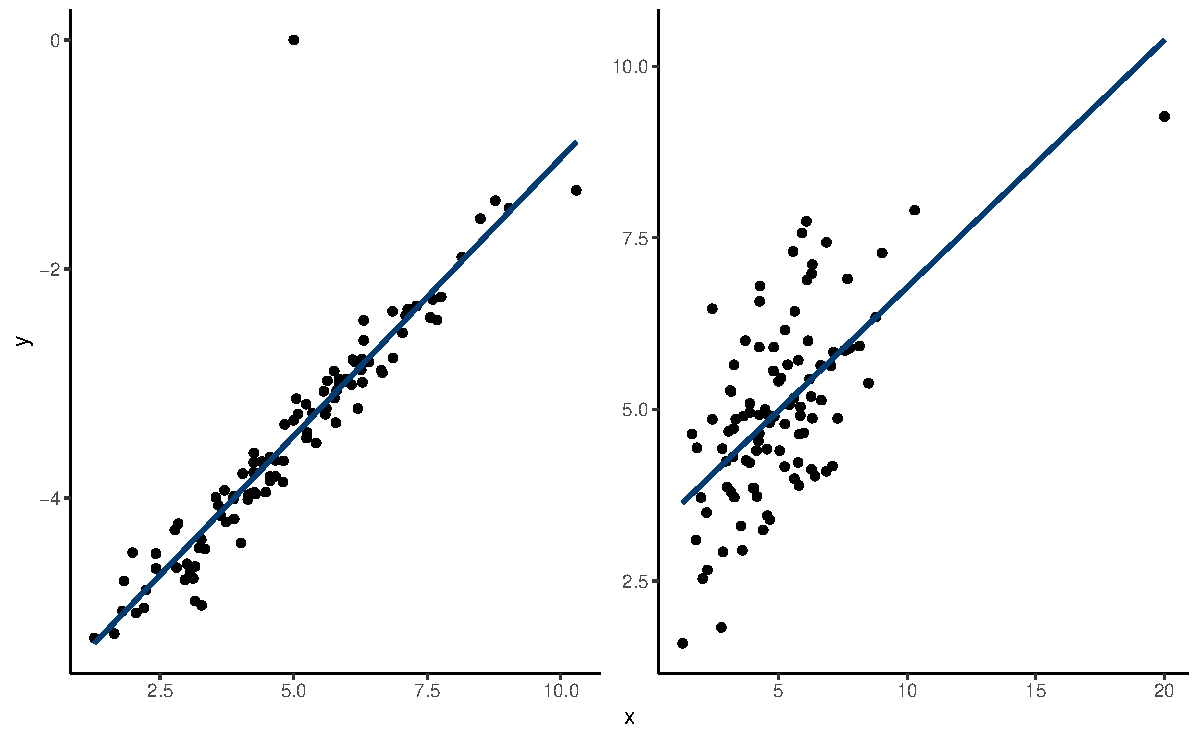
\includegraphics[width=0.85\textwidth,height=\textheight]{linearmodels_files/figure-pdf/fig-outliers-1.pdf}

}

\caption{\label{fig-outliers}Outlier and influential observation. The
left panel shows an outlier, whereas the right panel shows an
influential variable (rightmost \(x\) value).}

\end{figure}%

If influential observations can be detected by inspecting the leverage
of each observation, outliers are more difficult to diagnose.

An outlier stands out from the rest of the observations, either because
it has an usual response value, or because it falls far from the
regression surface. Loosely speaking, an outlier is an unusual values of
\(Y\) for a given combination of \(\mathbf{X}\) that stands out from the
rest. Outliers can be detected during the exploratory data analysis or
picked-up in residual plots (large values of \(|e_i|\) in plots of
fitted versus residuals) or added-variable plots. One could potentially
test whether an jackknife studentized residual is an outlier (adjusting
for the fact we would consider only largest values). One can also
consider Cook's distance, \(C_j\), a statistic giving the scaled
distance between the fitted values \(\hat{\boldsymbol{y}}\) and the
fitted values for the model with all but the \(j\)th observation,
\(\hat{\boldsymbol{y}}^{(-j)}\), \begin{align*}
C_j = \frac{1}{(p+1)S^2} \sum_{i=1}^n \left\{\hat{y}_i - \hat{y}_{i}^{(-j)}\right\}^2
\end{align*} Large values of \(C_j\) indicate that its residual \(e_j\)
is large relative to other observations or else its leverage \(h_j\) is
high. A rule of thumb is to consider points for which
\(C_j > 4/(n-p-1)\). In practice, if two observations are outlying and
lie in the same region, their Cook distance will be halved.

Outliers and influential observations should not be disregarded because
they don't comply with the model, but require further investigation.
They may motivate further modelling for features not accounted for. It
is also useful to check for registration errors in the data (which can
be safely discarded).

Except in obvious scenarios, unusual observations should not be
discarded. In very large samples, the impact of a single outlier is
hopefully limited. Transformations of the response may help reduce
outlyingness. Otherwise, alternative objective functions (as those
employed in robust regression) can be used; these downweight extreme
observations, at the cost of efficiency.

\section{Diagnostic plots}\label{diagnostic-plots}

We review the assumptions in turn and discuss what happens when the
assumptions fail to hold.

\subsection{Independence assumption}\label{independence-assumption}

Usually, the independence of the observations follows directly from the
type of sampling used --- this assumption is implicitly true if the
observations were taken from a \emph{random sample} from the population.
This is generally not the case for longitudinal data, which contains
repeated measures from the same individuals across time. Likewise, time
series are bound not to have independent observations. If we want to
include all the time points in the analysis, we must take into account
the possible dependence (correlation) between observations. If we ignore
correlation, the estimated standard errors are too small relative to the
truth, so the effective sample size is smaller than number of
observations.

What is the impact of dependence between measurements? Heuristically,
correlated measurements carry less information than independent ones. In
the most extreme case, there is no additional information and
measurements are identical, but adding them multiple times unduly
inflates the statistic and leads to more frequent rejections.

\begin{figure}[ht!]

\centering{

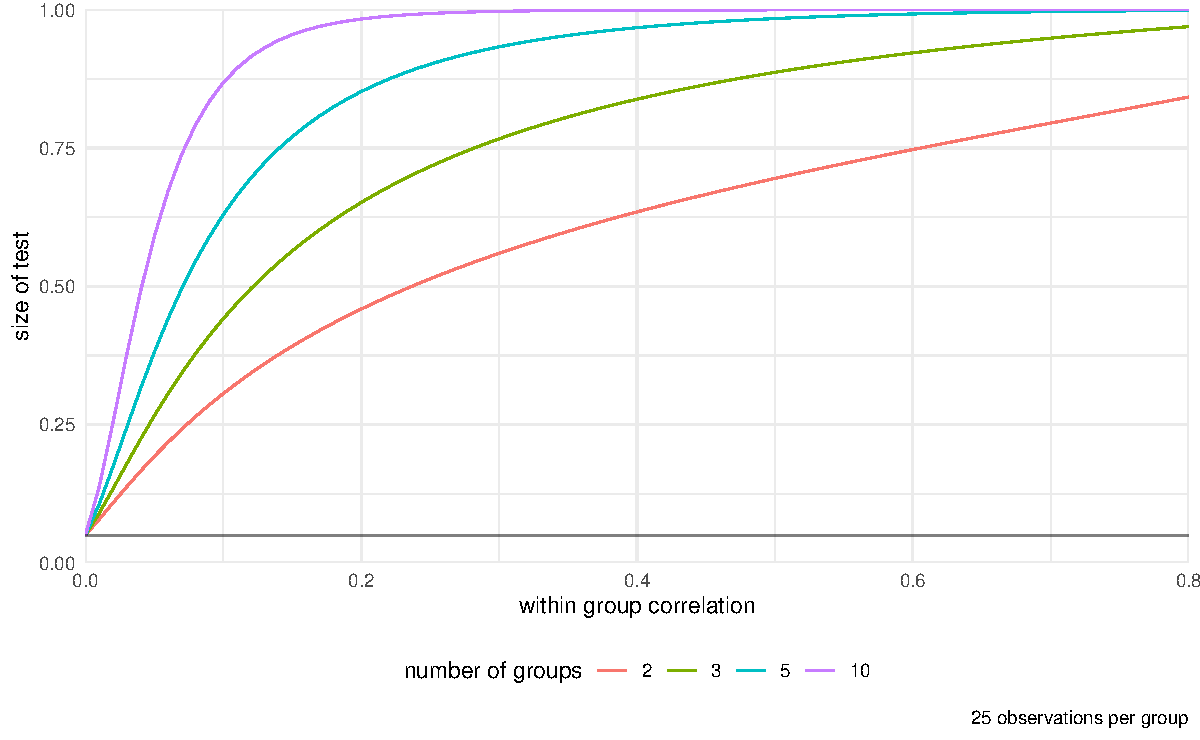
\includegraphics[width=0.85\textwidth,height=\textheight]{linearmodels_files/figure-pdf/fig-plotLevelIndep-1.pdf}

}

\caption{\label{fig-plotLevelIndep}Percentage of rejection of the null
hypothesis for the \(F\)-test of equality of means for the one way ANOVA
with data generated with equal mean and variance from an equicorrelation
model (within group observations are correlated, between group
observations are independent). The nominal level of the test is 5\%.}

\end{figure}%

The lack of independence can also have drastic consequences on inference
and lead to false conclusions: Figure~\ref{fig-plotLevelIndep} shows an
example with correlated samples within group (or equivalently repeated
measurements from individuals) with 25 observations per group. The
\(y\)-axis shows the proportion of times the null is rejected when it
shouldn't be. Here, since the data are generated from the null model
(equal mean) with equal variance, the inflation in the number of
spurious discoveries, false alarm or type I error is alarming and the
inflation is substantial even with very limited correlation between
measurements.

The first source of dependence is clustered data, meaning measurements
taken from subjects that are not independent from one another (family,
groups, etc.) More generally, correlation between observations can
arises from space-time dependence, roughly categorized into

\begin{itemize}
\tightlist
\item
  longitudinal data: repeated measurements are taken from the same
  subjects (few time points)
\item
  time series: observations observed at multiple time periods (many time
  points).
\end{itemize}

Time series require dedicated models not covered in this course. Because
of autocorrelation, positive errors tend to be followed by positive
errors, etc. We can plot the residuals as a function of time, and a
scatterplot of lagged residuals \(e_i\) versus \(e_{i-1}\)
(\(i=2, \ldots, n\)).

\begin{figure}[ht!]

\centering{

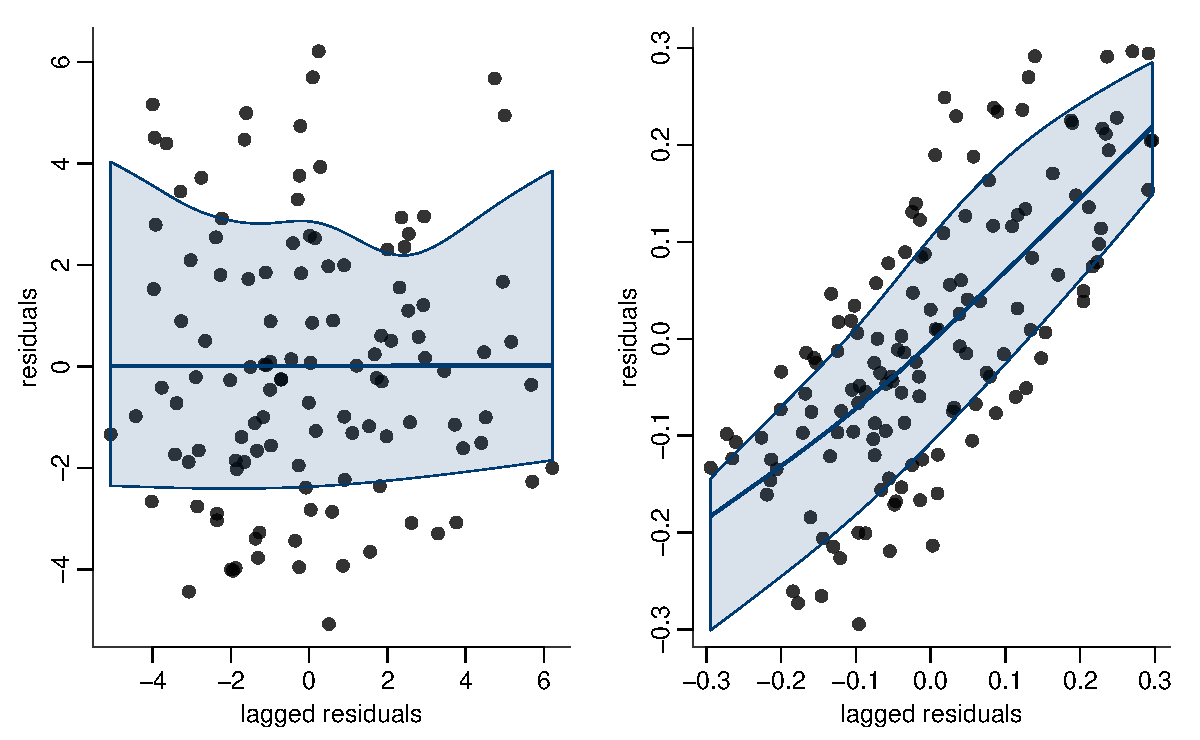
\includegraphics[width=0.85\textwidth,height=\textheight]{linearmodels_files/figure-pdf/fig-timeresidplot-1.pdf}

}

\caption{\label{fig-timeresidplot}Lagged residual plots: there is no
evidence against independence in the left panel, whereas the right panel
shows positively correlated residuals.}

\end{figure}%

However, lagged residuals plots only show dependence at lag one between
observations. For time series, we can look instead at a correlogram,
i.e., a bar plot of the correlation between two observations \(h\) units
apart as a function of the lag \(h\)
(\citeproc{ref-Brockwell.Davis:2016}{Brockwell and Davis 2016},
Definition 1.4.4).

For \(y_1, \ldots, y_n\) and constant time lags \(h=0, 1, \ldots\)
units, the autocorrelation at lag \(h\) is \begin{align*}
r(h) = \frac{\gamma(h)}{\gamma(0)}, \qquad \gamma(h) = \frac{1}{n}\sum_{i=1}^{n-|h|} (y_i-\overline{y})(y_{i+h}) - \overline{y})
\end{align*}

If the series is correlated, the sample autocorrelation will likely fall
outside of the pointwise confidence intervals, as shown in
Figure~\ref{fig-correlogram}. Presence of autocorrelation requires
modelling the correlation between observations explicitly using
dedicated tools from the time series literature. We will however examine
\(\mathsf{AR}(1)\) models as part of the chapter on longitudinal data.

When observations are positively correlated, the estimated standard
errors reported by the software are too small. This means we are
overconfident and will reject the null hypothesis more often then we
should if the null is true (inflated Type I error, or false positive).

\begin{figure}[ht!]

\centering{

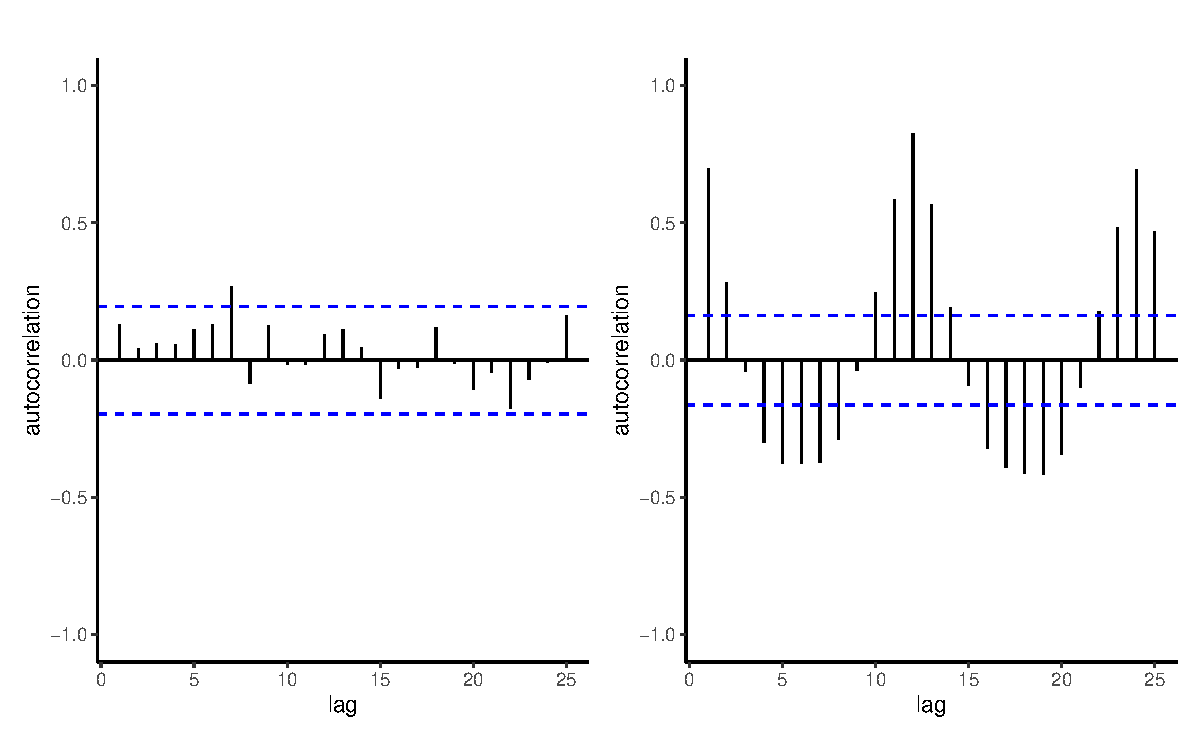
\includegraphics[width=0.85\textwidth,height=\textheight]{linearmodels_files/figure-pdf/fig-correlogram-1.pdf}

}

\caption{\label{fig-correlogram}Correlogram of independent observations
(left) and the ordinary residuals of the log-linear model fitted to the
air passengers data (right). While the mean model of the latter is
seemingly correctly specified, there is residual dependence between
monthly observations and yearly (at lag 12). The blue lines give
approximate pointwise 95\% confidence intervals for white noise
(uncorrelated observations).}

\end{figure}%

\subsection{Linearity assumption}\label{linearity-assumption}

The second assumption of the linear model is that of linearity, which
means that the mean model is correctly specified, all relevant
covariates have been included and their effect is correctly specified.
To check that the response surface of the linear model is adequate, we
plot \(e_i\) against \(\widehat{y}_i\) or \(\mathrm{X}_{ij}\) (for
\(j=1, \ldots, p\)). Since the linear correlation between
\(\boldsymbol{e}\) and \(\widehat{\boldsymbol{y}}\) (or
\(\boldsymbol{e}\) and \(\mathbf{X}_j\)) is zero by construction,
patterns (e.g., quadratic trend, cycles, changepoints) are indicative of
misspecification of the mean model. One can add a smoother to detect
patterns. Figure~\ref{fig-regdiaglin} shows three diagnostics plots, the
second of which shows no pattern in the residuals, but skewed fitted
values.

\begin{figure}[ht!]

\centering{

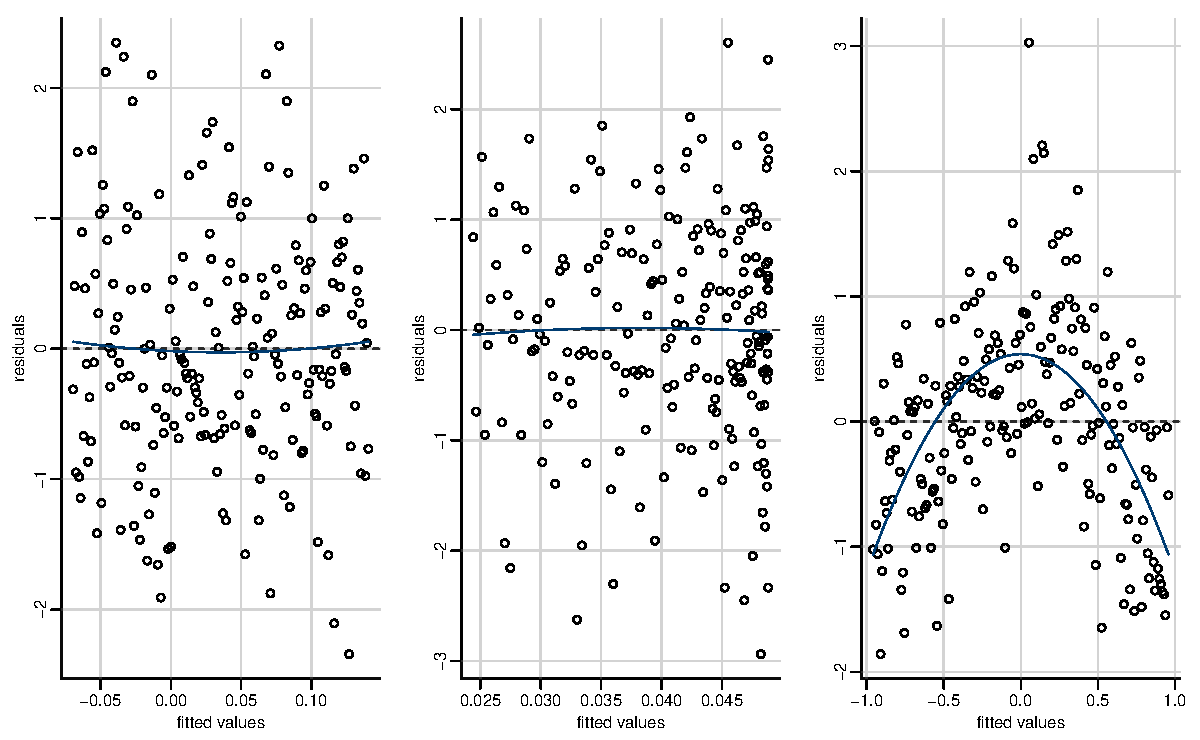
\includegraphics[width=0.85\textwidth,height=\textheight]{linearmodels_files/figure-pdf/fig-regdiaglin-1.pdf}

}

\caption{\label{fig-regdiaglin}Scatterplots of residuals against fitted
values. The first two plots show no departure from linearity (mean
zero). The third plot shows a clear quadratic pattern, suggesting the
mean model is misspecified. Note that the distribution of the fitted
value need not be uniform, as in the second panel which shows more high
fitted values.}

\end{figure}%

If there is residual structure in plots of ordinary residuals against
either (a) the fitted values or (b) the explanatory variables, a more
complex model can be adjusted including interactions, nonlinear
functions, \ldots If the effect of an explanatory variable is clearly
nonlinear and complicated, smooth terms could be added (we won't cover
generalized additive models in this course).

Plotting residuals against left-out explanatory variables can also serve
to check that all of the explanatory power of the omitted covariate is
already explained by the columns of \(\mathbf{X}\).

If an important variable has been omitted and is not available in the
dataset, then the effect of that variable is captured by both the errors
(the portion orthogonal to the model matrix \(\mathbf{X}\), i.e.,
unexplained by the covariates included in the model) and the remaining
part is captured by other explanatories of the model that are correlated
with the omitted variable. These variables can act as confounders. There
is little that can be done in either case unless the data for the
omitted variable are available, but subject-specific knowledge may help
make sense of the results.

\subsection{Constant variance
assumption}\label{constant-variance-assumption}

If the variance of the errors is the same for all observations
(homoscedasticity), that of the observations \(Y\) is also constant. The
most common scenarios for heteroscedasticity are increases in variance
with the response, or else variance that depends on explanatory
variables \(\mathbf{X}\), most notably categorical variables. For the
former, a log-transform (or Box--Cox transformation) can help stabilize
the variance, but we need the response to be positive. For the latter,
we can explicitly model that variance and we will see how to include
different variance per group later on. A popular strategy in the
econometrics literature, is to use robust (inflated) estimators of the
standard errors such as
\href{https://en.wikipedia.org/wiki/Heteroscedasticity-consistent_standard_errors}{White's
sandwich estimator of the variance}.

If the residuals (or observations) are heteroscedastic (non constant
variance), the estimated effects of the variables (the \(\beta\)
parameters) are still valid in the sense that the ordinary least squares
estimator \(\widehat{\boldsymbol{\beta}}\) is unbiased. However, the
estimated standard errors of the \(\widehat{\beta}\) are no longer
reliable and, consequently, the confidence intervals and the hypothesis
tests for the model parameters will be incorrect. Indeed, if the
variance of the errors differs from one observation to the next, we will
estimate an average of the different variance terms. The standard errors
of each term are incorrect (too small or too large) and the conclusions
of the tests (\(p\)-values) will be off because the formulas of both
\(t\)-test and \(F\)-test statistics include estimates of
\(\hat{\sigma}^2\).

Looking at the plot of jackknife studentized residuals against
regressors (or fitted values) is instructive --- for example, we often
see a funnel pattern when there is an increase in variance in the plot
of the jackknife studentized residuals against fitted value, or else in
boxplots with a categorical variable as in
Figure~\ref{fig-diagfitvalhomosce}. However, if we want to fit a local
smoother to observe trends, it is better to plot the absolute value of
the jackknife studentized residuals against regressors or observation
number.

\begin{figure}[ht!]

\centering{

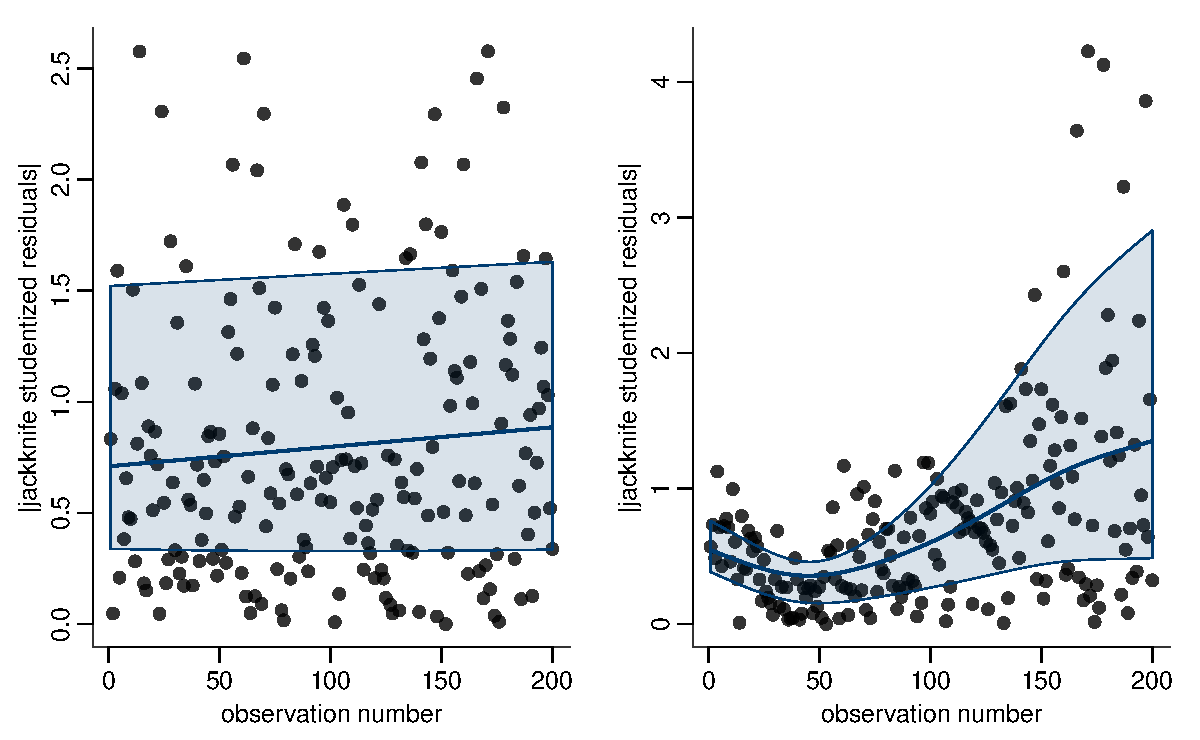
\includegraphics[width=0.85\textwidth,height=\textheight]{linearmodels_files/figure-pdf/fig-residhomoscedastic-1.pdf}

}

\caption{\label{fig-residhomoscedastic}Plot of the absolute value of
jackknife studentized residuals against observation number. The left
panel is typical of homoscedastic data, whereas the right panel
indicates an increase in the variance.}

\end{figure}%

\begin{figure}[ht!]

\centering{

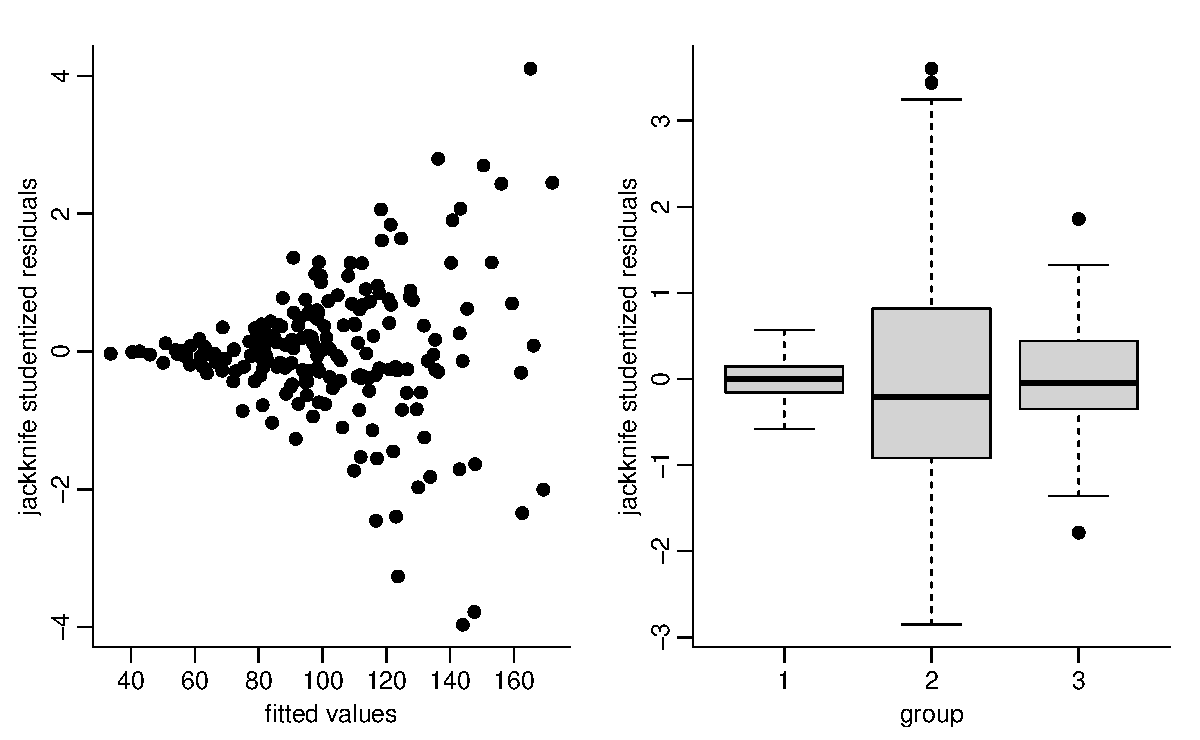
\includegraphics[width=0.85\textwidth,height=\textheight]{linearmodels_files/figure-pdf/fig-diagfitvalhomosce-1.pdf}

}

\caption{\label{fig-diagfitvalhomosce}Plot of jackknife studentized
residuals against fitted value (left) and categorical explanatory
(right). Both clearly display heteroscedasticity.}

\end{figure}%

An obvious extension of the linear model is to allow variance to vary
according to explanatories, typically categorical covariates. In a
likelihood framework, this is easy to do and we will cover this approach
in more detail.

We can perform hypothesis tests for the homogeneity (equal) variance
assumption. The most commonly used tests are Bartlett's test, the
likelihood ratio test under the assumption of normally distributed data,
with a Bartlett correction to improve the \(\chi^2\) approximation to
the null distribution. The second most popular is Levene's test (a more
robust alternative, less sensitive to outliers). For both tests, the
null distribution is \(\mathscr{H}_0: \sigma^2_1 = \cdots = \sigma^2_K\)
against the alternative that at least two differ. The Bartlett test
statistic has a \(\chi^2\) null distribution with \(K-1\) degrees of
freedom, whereas Levene's test has an \(F\)-distribution with (\(K-1\),
\(n-K\)) degrees of freedom: it is equivalent to computing the one-way
ANOVA \(F\)-statistic with the absolute value of the centered residuals,
\(|y_{ik} - \widehat{\mu}_k|\), as observations.

What are the impacts of unequal variance if we use the \(F\)-test
instead? For one, the pooled variance will be based on a weighted
average of the variance in each group, where the weight is a function of
the sample size. This can lead to size distortion (meaning that the
proportion of type I error is not the nominal level \(\alpha\) as
claimed) and potential loss of power. The following toy example
illustrates this.

\begin{example}[Violation of the null hypothesis of equal
variance]\protect\hypertarget{exm-heterogeneity}{}\label{exm-heterogeneity}

~

\begin{figure}[ht!]

\centering{

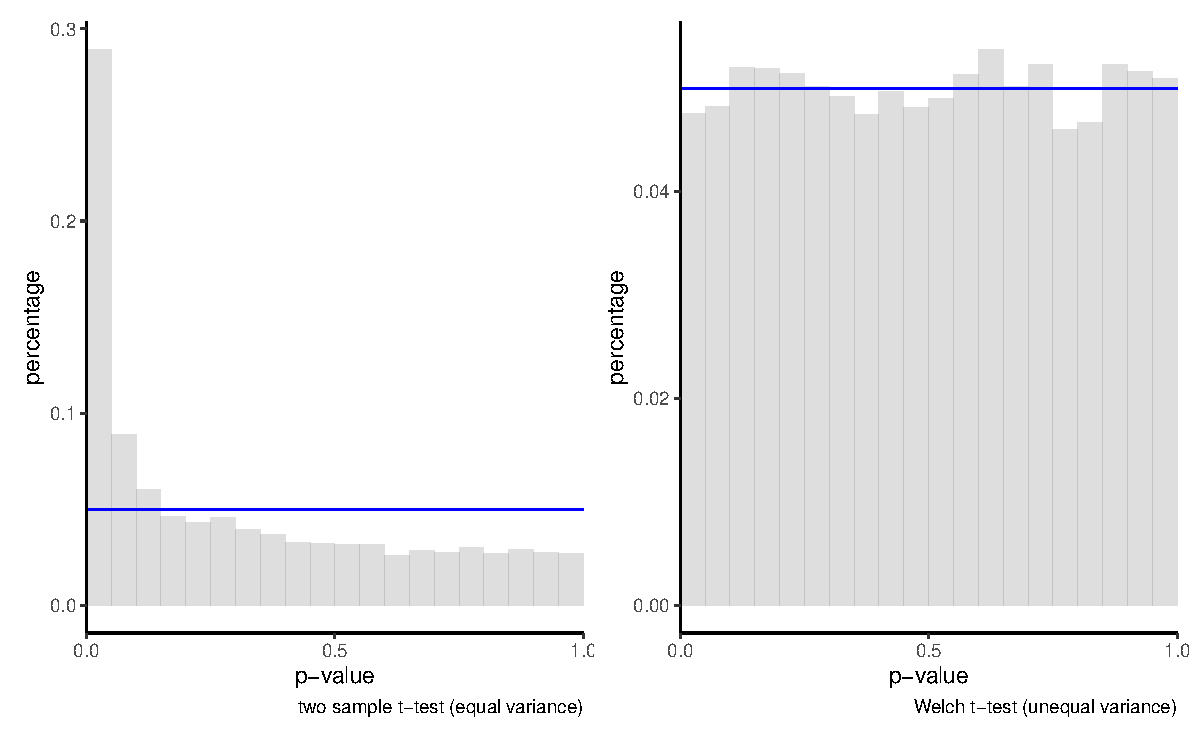
\includegraphics[width=0.85\textwidth,height=\textheight]{linearmodels_files/figure-pdf/fig-simuWelchnull-1.pdf}

}

\caption{\label{fig-simuWelchnull}Histogram of the null distribution of
\(p\)-values obtained through simulation using the classical analysis of
variance \(F\)-test (left) and Welch's unequal variance alternative
(right), based on 10 000 simulations. Each simulated sample consist of
50 observations from a \(\mathsf{Normal}(0, 1)\) distribution and 10
observations from \(\mathsf{Normal}(0, 9)\). The uniform distribution
would have 5\% in each of the 20 bins used for the display.}

\end{figure}%

We consider for simplicity a problem with \(K=2\) groups, which is the
two-sample \(t\)-test. We simulated 50 observations from a
\(\mathsf{Normal}(0, 1)\) distribution and 10 observations from
\(\mathsf{Normal}(0, 9)\), comparing the distribution of the
\(p\)-values for the Welch and the \(F\)-test statistics.
Figure~\ref{fig-simuWelchnull} shows the results. The percentage of
\(p\)-values less than \(\alpha=0.05\) based on 10 000 replicates is
estimated to be 4.76\% for the Welch statistic, not far from the level.
By contrast, we reject 28.95\% of the time with the one-way ANOVA global
\(F\)-test: this is a large share of innocents sentenced to jail based
on false premises! While the size distortion is not always as striking,
heterogeneity should be accounted in the design by requiring sufficient
sample sizes (whenever costs permits) in each group to be able to
estimate the variance reliably and using an adequate statistic.

\end{example}

There are alternative graphical ways of checking the assumption of equal
variance, many including the standardized residuals
\(r_{ik} = (y_{ik} - \widehat{\mu}_k)/\widehat{\sigma}\) against the
fitted values \(\widehat{\mu}_k\). We will cover these in later
sections.

Oftentimes, unequal variance occurs because the model is not additive.
You could use variance-stabilizing transformations (e.g., log for
multiplicative effects) to ensure approximately equal variance in each
group. Another option is to use a model that is suitable for the type of
response you have (including count and binary data). Lastly, it may be
necessary to explicitly model the variance in more complex design
(including repeated measures) where there is a learning effect over time
and variability decreases as a result. Consult an expert if needed.

\subsection{Normality assumption}\label{normality-assumption}

The normality assumption is mostly for convenience: if the errors are
assumed normally distributed, then the least square and the maximum
likelihood estimators of \(\boldsymbol{\beta}\) coincide. The maximum
likelihood estimators of \(\boldsymbol{\beta}\) are asymptotically
normal under mild conditions on the model matrix and \(t\)-tests are
surprisingly robust and unaffected by departure from the normality
assumption. This means that inference is valid in large samples,
regardless of the distribution of the errors/residuals (even if the null
distribution are not exact). It is important to keep in mind that, for
categorical explanatory variables, the sample size in each group must be
sufficiently large for the central limit theorem to kick in since
coefficients represent group average.

Sometimes, transformations can improve normality: if the data is
right-skewed and the response is strictly positive, a log-linear model
may be more adequate Section~\ref{sec-transfo}. This can be assessed by
looking at the quantile-quantile plot of the externally studentized
residuals. If the response \(Y\) is not continuous (including binary,
proportion or count data), linear models give misleading answers and
generalized linear models are more suitable.

The inference will be valid for large samples even if the errors are not
normally distributed by virtue of the central limit theorem. If the
errors \(\varepsilon_i \sim \mathsf{normal}(0, \sigma^2)\), then the
jacknnife studentized residuals should follow a Student distribution,
with \(r_i \sim \mathsf{Student}(n-p-2)\), (identically distributed, but
not independent). A Student quantile-quantile plot can thus be used to
check the assumption (and for \(n\) large, the normal plotting positions
could be used as approximation if \(n-p> 50\)). One can also plot a
histogram of the residuals. Keep in mind that if the mean model is not
correctly specified, some residuals may incorporate effect of leftover
covariates.

\begin{figure}[ht!]

\centering{

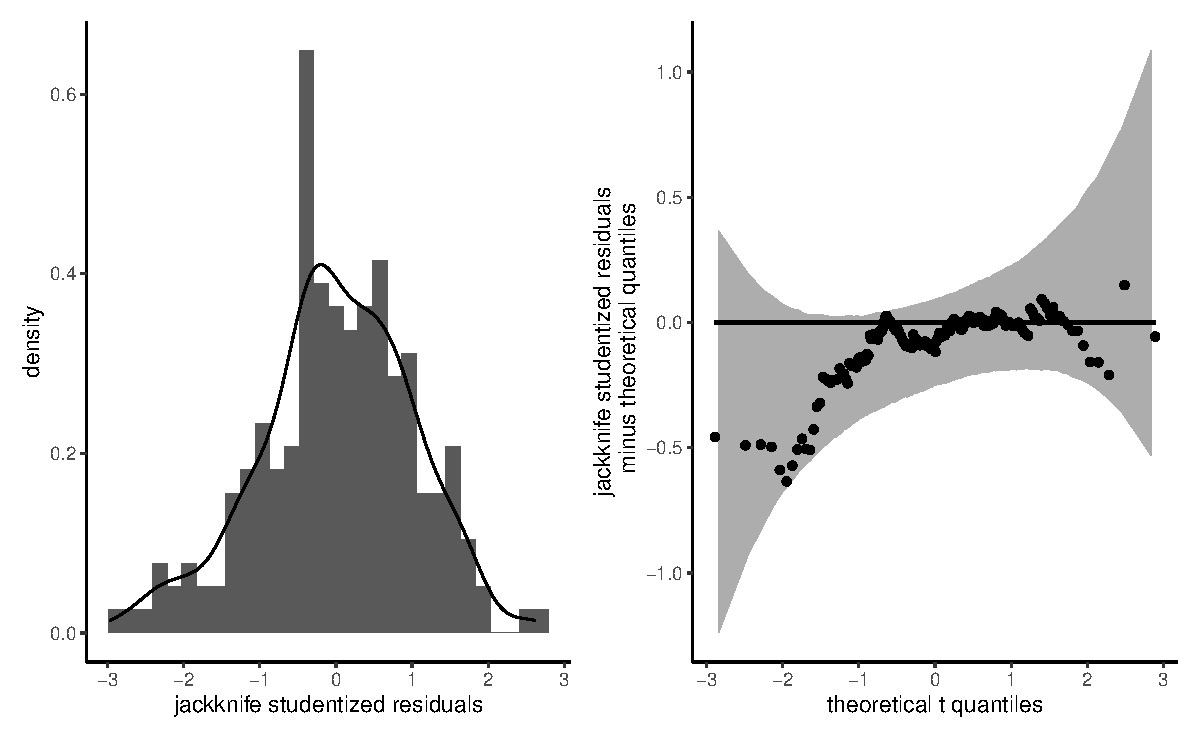
\includegraphics[width=0.85\textwidth,height=\textheight]{linearmodels_files/figure-pdf/fig-qqplotresid-1.pdf}

}

\caption{\label{fig-qqplotresid}Histogram (left) and Student
quantile-quantile plot (right) of the jackknife studentized residuals.
The left panel includes a kernel density estimate (black), with the
density of Student distribution (blue) superimposed. The right panel
includes pointwise 95\% confidence bands calculated using a bootstrap.}

\end{figure}%

Quantile-quantile plots are discussed in Definition~\ref{def-qqplot} but
their interpretation requires training. For example,
Figure~\ref{fig-qqplotsbad} shows many common scenarios that can be
diagnosed using quantile-quantile plots: discrete data is responsible
for staircase patterns, positively skewed data has too high low
quantiles and too low high quantiles relative to the plotting positions,
heavy tailed data have high observations in either tails and bimodal
data leads to jumps in the plot.

\begin{figure}[ht!]

\centering{

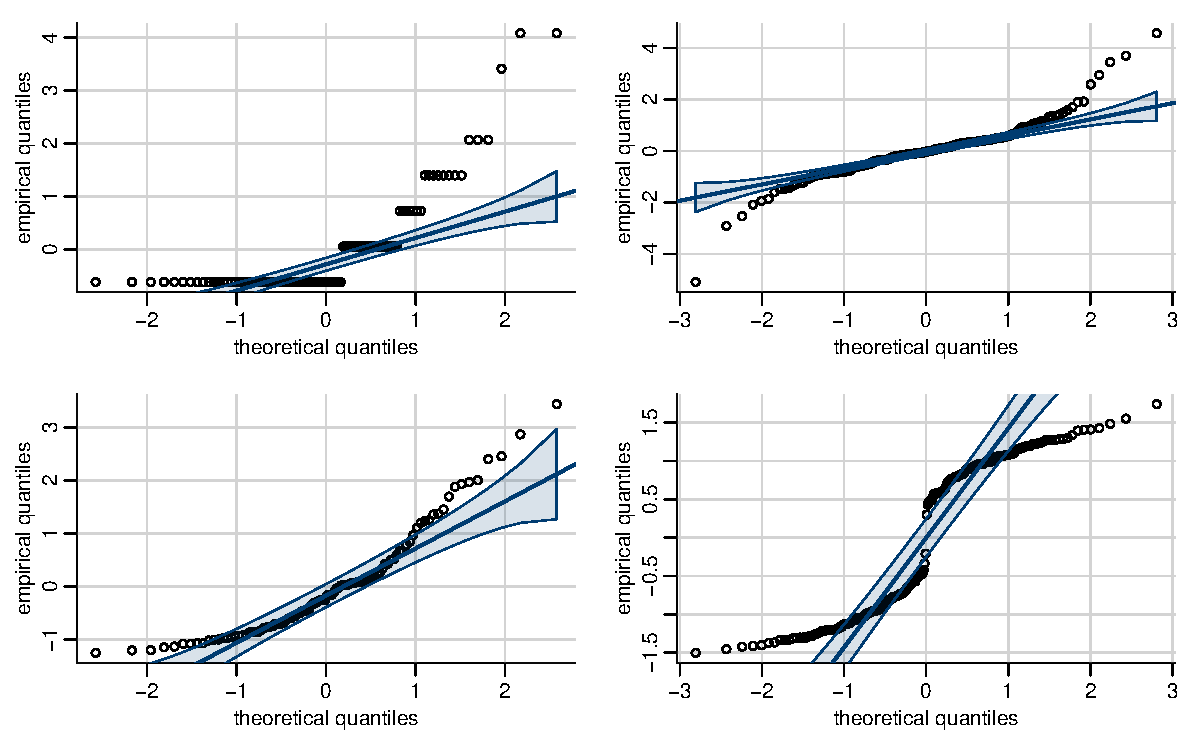
\includegraphics[width=0.85\textwidth,height=\textheight]{linearmodels_files/figure-pdf/fig-qqplotsbad-1.pdf}

}

\caption{\label{fig-qqplotsbad}Quantile-quantile plots of non-normal
data, showing typical look of behaviour of discrete (top left), heavy
tailed (top right), skewed (bottom left) and bimodal data (bottom
right).}

\end{figure}%

\begin{example}[Diagnostic plots for the \(\texttt{college}\)
data.]\protect\hypertarget{exm-diagplotcollege}{}\label{exm-diagplotcollege}

We can look at the \texttt{college} data to see if the linear model
assumptions hold.

\begin{figure}[ht!]

\centering{

\includegraphics[width=0.85\textwidth,height=\textheight]{linearmodels_files/figure-pdf/fig-diagplotscollege-1.pdf}

}

\caption{\label{fig-diagplotscollege}Diagnostic plots for the college
data example: ordinary residuals against fitted values (top left),
absolute value of the jacknnife studentized residuals against fitted
values (top right), box and whiskers plot of jacknnife studentized
residuals (bottom left) and detrended Student quantile-quantile plot
(bottom right). There is clear group heteroscedasticity.}

\end{figure}%

Based on the plots of Figure~\ref{fig-diagplotscollege}, we find that
there is residual heteroscedasticity, due to rank. Since the number of
years in the first rank is limited and all assistant professors were
hired in the last six years, there is less disparity in their income. It
is important not to mistake the pattern on the \(x\)-axis for the fitted
value (due to the large effect of rank and field, both categorical
variable) with patterns in the residuals (none apparent). Fixing the
heteroscedasticity would correct the residuals and improve the
appearance of the quantile-quantile plot.

\end{example}

\section{Extensions of the model}\label{extensions-of-the-model}

\subsection{Transformation of the response}\label{sec-transfo}

If the response is strictly positive, there are some options that can
alleviate lack of additivity, more specifically multiplicative
mean-variance relationships.If the data is right-skewed and the response
is strictly positive, a log-linear model may be more adequate and the
parameters can be interpreted. Theory sometimes dictates a
multiplicative model: for example, the Cobb--Douglas production function
in economics is \(P=\alpha L^{\beta_1}C^{\beta_2}\), where \(P\) stands
for production, \(L\) for labor and \(C\) for capital; all inputs are
positive, so taking a log-transform yields a model that is linear in
\(\beta\), with \(\beta_0=\ln(\alpha)\).

We can rewrite the log-linear model in the original response scale as
\begin{align*}
Y = \exp\left(\beta_0+\sum_{j=1}^p\beta_jX_j +  \varepsilon \right) \\&= \exp\left(\beta_0+ \sum_{j=1}^p\beta_jX_j\right)\cdot \exp(\varepsilon),
\end{align*} and thus \begin{align*}
\mathsf{E}(Y \mid \mathbf{X}) = \exp(\beta_0 +\beta_1 X_1 +\cdots + \beta_pX_p) \times \mathsf{E}\{\exp(\varepsilon) \mid \mathbf{X}\}.
\end{align*}

If \(\varepsilon \mid \mathbf{X} \sim \mathsf{normal}(\mu,\sigma^2)\),
then
\(\mathsf{E}\{\exp(\varepsilon) \mid \mathbf{X}\}= \exp(\mu+\sigma^2/2)\)
and \(\exp(\varepsilon)\) follows a log-normal distribution.

An increase of one unit of \(X_j\) leads to a \(\beta_j\) increase of
\(\ln Y\) without interaction or nonlinear term for \(X_j\), and this
translates into a multiplicative increase of a factor \(\exp(\beta_j)\)
on the original data scale for \(Y\). Indeed, we can compare the ratio
of \(\mathsf{E}(Y \mid X_1=x+1)\) to \(\mathsf{E}(Y \mid X_1=x)\),
\begin{align*}
\frac{\mathsf{E}(Y \mid X_1=x+1, X_2, \ldots, X_p)}{\mathsf{E}(Y \mid X_1=x,  X_2, \ldots, X_p)} = \frac{\exp\{\beta_1(x+1)\}}{\exp(\beta_1 x)} = \exp(\beta_1).
\end{align*} Thus, \(\exp(\beta_1)\) represents the ratio of the mean of
\(Y\) when \(X_1=x+1\) in comparison to that when \(X_1=x\),
\emph{ceteris paribus} (and provided this statement is meaningful). If
\(\beta_j=0\), the multiplicative factor one is the identity, whereas
negative values of the regression coefficient \(\beta_j<0\) leads to
\(\exp(\beta_j)<1\). The percentage change is \(1-\exp(\beta_j)\) if
\(\beta_j <0\) and \(\exp(\beta_j)-1\) if \(\beta_j>0\)

Sometimes, we may wish to consider a log transformation of both the
response and some of the continuous positive explanatories, when this
make sense (a so-called log-log model). Consider the case where both
\(Y\) and \(X_1\) is log-transformed, so the equation for the mean on
the original data scale reads \begin{align*}
Y= X_1^{\beta_1}\exp(\beta_0 + \beta_2X_2 + \cdots + \beta_pX_p + \varepsilon)
\end{align*} Taking the derivative of the left hand side with respect to
\(X_1>0\), we get \begin{align*}
\frac{\partial Y}{\partial X_1}&= \beta_1 X_1^{\beta_1-1}\exp(\beta_0 + \beta_2X_2 + \cdots + \beta_pX_p + \varepsilon)
\\&= \frac{\beta_1 Y}{X_1}
\end{align*} and thus we can rearrange the expression so that
\begin{align*}
\frac{\partial X_1}{X_1}\beta_1 = \frac{\partial Y}{Y};
\end{align*} this is a partial \textbf{elasticity}, so \(\beta_1\) is
interpreted as a \(\beta_1\) percentage change in \(Y\) for each
percentage increase of \(X_1\), \emph{ceteris paribus}.

\begin{example}[Log-log
model]\protect\hypertarget{exm-loglog}{}\label{exm-loglog}

Consider for example the Cobb--Douglas production function
(\citeproc{ref-Douglas:1976}{Douglas 1976}), which specifies that
economic output \(Y\) is related to labour \(L\) and capital \(C\) via
\(\mathsf{E}(Y \mid L, C) = \beta_0C^{\beta}L^{1-\beta}\) with
\(\beta \in (0,1)\). If we take logarithms on both sides (since all
arguments are positive), then
\(\mathsf{E}(\ln Y \mid L, C) = \beta_0^* + \beta_1 \ln C + (1-\beta_1)\ln L\).
We could fit a linear model with response \(\ln Y - \ln L\) and
explanatory variable \(\ln C - \ln L\), to obtain an estimate of the
coefficient \(\beta_1\), while \(\beta_0^*=\ln \beta_0\). A constrained
optimization would be potentially necessary to estimate the model
parameters of the resulting linear model if the estimates lie outside of
the parameter space.

\end{example}

\begin{proposition}[Box--Cox
transformation]\protect\hypertarget{prp-boxcox}{}\label{prp-boxcox}

If the data are strictly positive, one can consider a Box--Cox
transformation, \begin{align*}
y(\lambda)= \begin{cases}
(y^{\lambda}-1)/\lambda, & \lambda \neq 0\\
\ln(y), & \lambda=0.
\end{cases}
\end{align*} The cases \(\lambda=-1\) (inverse), \(\lambda=1\)
(identity) and \(\lambda=0\) (log-linear model) are perhaps the most
important because they yield interpretable models.

If we assume that
\(\boldsymbol{Y}(\lambda) \sim \mathsf{normal}(\mathbf{X}\boldsymbol{\beta}, \sigma^2 \mathbf{I}_n)\),
then the likelihood is \begin{align*}
L(\lambda, \boldsymbol{\beta}, \sigma; \boldsymbol{y}, \mathbf{X}) &= (2\pi\sigma^2)^{-n/2} J(\lambda, \boldsymbol{y}) \times\\& \quad \exp \left[ - \frac{1}{2\sigma^2}\{\boldsymbol{y}(\lambda) - \mathbf{X}\boldsymbol{\beta}\}^\top\{\boldsymbol{y}(\lambda) - \mathbf{X}\boldsymbol{\beta}\}\right],
\end{align*} where \(J\) denotes the Jacobian of the Box--Cox
transformation,
\(J(\lambda, \boldsymbol{y})=\prod_{i=1}^n y_i^{\lambda-1}\). For each
given value of \(\lambda\), the maximum likelihood estimator is that of
the usual regression model, with \(\boldsymbol{y}\) replaced by
\(\boldsymbol{y}(\lambda)\), namely
\(\widehat{\boldsymbol{\beta}}_\lambda = (\mathbf{X}^\top\mathbf{X})^{-1}\mathbf{X}^\top \boldsymbol{y}(\lambda)\)
and
\(\widehat{\sigma}^2_\lambda = n^{-1}\{ \boldsymbol{y}(\lambda) - \mathbf{X}\widehat{\boldsymbol{\beta}}_\lambda\}^\top\{ \boldsymbol{y}(\lambda) - \mathbf{X}\widehat{\boldsymbol{\beta}}_\lambda\}\).

The profile log likelihood is \begin{align*}
\ell_{\mathsf{p}}(\lambda) = -\frac{n}{2}\ln(2\pi \widehat{\sigma}^2_\lambda) - \frac{n}{2} + (\lambda - 1)\sum_{i=1}^n \ln(y_i)
\end{align*} The maximum profile likelihood estimator is the value
\(\lambda\) minimizes the sum of squared residuals from the linear model
with \(\boldsymbol{y}(\lambda)\) as response.

The Box--Cox is not a panacea and should be reserved to cases where the
transformation reduces heteroscedasticity (unequal variance) or creates
a linear relation between explanatories and response: theory provides a
cogent explanation of the data. Rather than an \emph{ad hoc} choice of
transformation, one could choose a log transformation if the value \(0\)
is included within the 95\% confidence interval since this improves
interpretability.

\end{proposition}

\begin{example}[Box--Cox transform for the \texttt{poison}
data]\protect\hypertarget{exm-poisonboxcox}{}\label{exm-poisonboxcox}

Box and Cox (\citeproc{ref-Box.Cox:1964}{1964}) considered survival time
for 48 animals based on a randomized trial; these data are analyzed in
Example 8.25 of Davison (\citeproc{ref-Davison:2003}{2003}). Three
poisons were administered with four treatments; each factor combination
contained four animals, chosen at random. There is strong evidence that
both the choice of poison and treatment affect survival time.

We could consider a two-way analysis of variance model for these data
without interaction, given the few observations for each combination.
The model would be of the form \begin{align*}
Y &= \beta_0 + \beta_1 \texttt{poison}_2 + \beta_2\texttt{poison}_3  +\beta_3\texttt{treatment}_2 \\ &\qquad+ \beta_4\texttt{treatment}_3
+\beta_5\texttt{treatment}_4 + \varepsilon
\end{align*}

The plot of fitted values against residuals shows that the model is not
additive; there is also indications that the variance increases with the
mean response. The model is inadequate: lowest survival times are
underpredicted, meaning the residuals are positive and likewise the
middle responses is positive. A formal test of non-additivity based on
constructed variables further point towards non-additivity
(\citeproc{ref-Davison:2003}{Davison 2003}, Example 8.24). Overall, the
model fit is poor and any conclusion drawn from it dubious.

One could consider using a Box--Cox to find a suitable transformation of
the residuals so as to improve normality. The profile log likelihood at
the bottom left of Figure~\ref{fig-poisonplots} suggests that
\(\lambda\approx -1\) would be a good choice. This has the benefit of
being interpretable, as the reciprocal response \(Y^{-1}\) corresponds
to the speed of action of the poison depending on both poison type and
treatment. The diagnostics plots also indicate that the model for the
reciprocal has no residual structure and the variance appears constant.

\begin{figure}[ht!]

\centering{

\includegraphics[width=0.85\textwidth,height=\textheight]{linearmodels_files/figure-pdf/fig-poisonplots-1.pdf}

}

\caption{\label{fig-poisonplots}Diagnostic plots for the poison data.
The top panel shows the ordinary residuals for the linear model for
survival time as a function of poison and treatment, with jittered
observations. The middle left plot shows the fitted values against
residuals, which display evidence of trend and increase in variance with
the survival time. The quantile-quantile plot in the middle right plot
shows some evidence of departure from the normality, but the
non-linearity and heteroscedasticity obscure this. The bottom panel
shows the profile log likelihood for the Box--Cox transform, suggesting
a value of \(-1\) would be within the 95\% confidence interval. After
fitting the same additive model with main effect only to the reciprocal
survival time, there is no more evidence of residual structure and
unequal variance.}

\end{figure}%

\end{example}

\section{Concluding remarks}\label{concluding-remarks}

Linear regression is the most famous and the most widely used
statistical model around. The name may appear reductive, but many tests
statistics (\emph{t}-tests, ANOVA, Wilcoxon, Kruskal--Wallis)
\href{https://lindeloev.github.io/tests-as-linear/linear_tests_cheat_sheet.pdf}{can
be formulated using a linear regression}, while
\href{https://threadreaderapp.com/thread/1286420597505892352.html}{models
as diverse as trees, principal components and deep neural networks are
just linear regression model in disguise}. What changes under the hood
between one fancy model to the next are the optimization method (e.g.,
ordinary least squares, constrained optimization or stochastic gradient
descent) and the choice of explanatory variables entering the model
(spline basis for nonparametric regression, indicator variable selected
via a greedy search for trees, activation functions for neural
networks).

\bookmarksetup{startatroot}

\chapter*{Bibliography}\label{bibliography}
\addcontentsline{toc}{chapter}{Bibliography}

\markboth{Bibliography}{Bibliography}

\phantomsection\label{refs}
\begin{CSLReferences}{1}{0}
\bibitem[\citeproctext]{ref-Baumann:1992}
Baumann, James F., Nancy Seifert-Kessell, and Leah A. Jones. 1992.
{``Effect of Think-Aloud Instruction on Elementary Students'
Comprehension Monitoring Abilities.''} \emph{Journal of Reading
Behavior} 24 (2): 143--72.
\url{https://doi.org/10.1080/10862969209547770}.

\bibitem[\citeproctext]{ref-Box.Cox:1964}
Box, G. E. P., and D. R. Cox. 1964. {``An Analysis of
Transformations.''} \emph{Journal of the Royal Statistical Society:
Series B (Methodological)} 26 (2): 211--43.
\url{https://doi.org/10.1111/j.2517-6161.1964.tb00553.x}.

\bibitem[\citeproctext]{ref-Brockwell.Davis:2016}
Brockwell, P. J., and R. A. Davis. 2016. \emph{Introduction to Time
Series and Forecasting}. Springer Texts in Statistics. Springer.

\bibitem[\citeproctext]{ref-Brodeur:2021}
Brodeur, Mathieu, Perrine Ruer, Pierre-Majorique Léger, and Sylvain
Sénécal. 2021. {``Smartwatches Are More Distracting Than Mobile Phones
While Driving: Results from an Experimental Study.''} \emph{Accident
Analysis \& Prevention} 149: 105846.
\url{https://doi.org/10.1016/j.aap.2020.105846}.

\bibitem[\citeproctext]{ref-Brucks.Levav:2022}
Brucks, Melanie S., and Jonathan Levav. 2022. {``Virtual Communication
Curbs Creative Idea Generation.''} \emph{Nature} 605 (7908): 108--12.
\url{https://doi.org/10.1038/s41586-022-04643-y}.

\bibitem[\citeproctext]{ref-Davison:2003}
Davison, A. C. 2003. \emph{Statistical Models}. Cambridge University
Press.

\bibitem[\citeproctext]{ref-Douglas:1976}
Douglas, Paul H. 1976. {``The {Cobb--Douglas} Production Function Once
Again: Its History, Its Testing, and Some New Empirical Values.''}
\emph{Journal of Political Economy} 84 (5): 903--15.
\url{http://www.jstor.org/stable/1830435}.

\bibitem[\citeproctext]{ref-Duke.Amir:2023}
Duke, Kristen E., and On Amir. 2023. {``The Importance of Selling
Formats: When Integrating Purchase and Quantity Decisions Increases
Sales.''} \emph{Marketing Science} 42 (1): 87--109.
\url{https://doi.org/10.1287/mksc.2022.1364}.

\bibitem[\citeproctext]{ref-Fox:1992}
Fox, John, and Georges Monette. 1992. {``Generalized Collinearity
Diagnostics.''} \emph{Journal of the American Statistical Association}
87 (417): 178--83. \url{https://doi.org/10.1080/01621459.1992.10475190}.

\bibitem[\citeproctext]{ref-Student:1908}
Gosset, William Sealy. 1908. {``The Probable Error of a Mean.''}
\emph{Biometrika} 6 (1): 1--25.
\url{https://doi.org/10.1093/biomet/6.1.1}.

\bibitem[\citeproctext]{ref-Lee.Choi:2019}
Lee, Kiljae, and Jungsil Choi. 2019. {``Image-Text Inconsistency Effect
on Product Evaluation in Online Retailing.''} \emph{Journal of Retailing
and Consumer Services} 49: 279--88.
\url{https://doi.org/10.1016/j.jretconser.2019.03.015}.

\bibitem[\citeproctext]{ref-Liu.Rim.Min.Min:2023}
Liu, Peggy J., SoYon Rim, Lauren Min, and Kate E. Min. 2023. {``The
Surprise of Reaching Out: Appreciated More Than We Think.''}
\emph{Journal of Personality and Social Psychology} 124 (4): 754--71.
\url{https://doi.org/10.1037/pspi0000402}.

\bibitem[\citeproctext]{ref-Moon.VanEpps:2023}
Moon, Alice, and Eric M VanEpps. 2023. {``Giving Suggestions: Using
Quantity Requests to Increase Donations.''} \emph{Journal of Consumer
Research} 50 (1): 190--210. \url{https://doi.org/10.1093/jcr/ucac047}.

\bibitem[\citeproctext]{ref-Rosen:1974}
Rosen, B., and T. H. Jerdee. 1974. {``Influence of Sex Role Stereotypes
on Personnel Decisions.''} \emph{Journal of Applied Psychology} 59:
9--14.

\bibitem[\citeproctext]{ref-Sokolova:2023}
Sokolova, Tatiana, Aradhna Krishna, and Tim Döring. 2023. {``Paper Meets
Plastic: The Perceived Environmental Friendliness of Product
Packaging.''} \emph{Journal of Consumer Research} 50 (3): 468--91.
\url{https://doi.org/10.1093/jcr/ucad008}.

\bibitem[\citeproctext]{ref-Venables:2000}
Venables, William N. 2000. {``Exegeses on Linear Models.''} In
\emph{S-PLUS User's Conference}. Washington, D.C.
\url{https://www.stats.ox.ac.uk/pub/MASS3/Exegeses.pdf}.

\end{CSLReferences}


\backmatter


\end{document}
